\documentclass{report}
\usepackage{german}
\usepackage[latin1]{inputenc}
\usepackage{a4wide}
\usepackage{epsfig}
\usepackage{amssymb}
\usepackage{amsmath}
\usepackage{enumerate}
\usepackage{fancyvrb}
\usepackage{alltt}
\usepackage{fleqn}
\usepackage{epic}
\usepackage{color} 
\usepackage{theorem}
\usepackage{hyperref}
\usepackage[all]{hypcap}
\hypersetup{
        colorlinks = true, % comment this to make xdvi work
        linkcolor  = blue,
        citecolor  = red,
        filecolor  = [rgb]{0.1, 0.1, 1.0},
        urlcolor   = [rgb]{0.1, 0.1, 1.0},
        pdfborder  = {0 0 0} 
}

\usepackage{fancyhdr}
\usepackage{lastpage} 

\pagestyle{fancy}

\fancyfoot[C]{--- \thepage/\pageref{LastPage}\ ---}

\fancypagestyle{plain}{%
\fancyhf{}
\fancyfoot[C]{--- \thepage/\pageref{LastPage}\ ---}
\renewcommand{\headrulewidth}{0pt}
}

\renewcommand{\chaptermark}[1]{\markboth{\chaptername \ \thechapter.\ #1}{}}
\renewcommand{\sectionmark}[1]{\markright{\thesection. \ #1}{}}
\fancyhead[R]{\leftmark}
\fancyhead[L]{\rightmark}

\definecolor{amethyst}{rgb}{0.2, 0.4, 0.6}
\definecolor{orange}{rgb}{1, 0.9, 0.0}

\usepackage[german]{babel}
\usepackage{babelbib}
\bibliographystyle{babunsrt}

{\theorembodyfont{\sf}
\newtheorem{Definition}{Definition}
\newtheorem{Axiom}[Definition]{Axiom}
\newtheorem{Notation}[Definition]{Notation}
\newtheorem{Korollar}[Definition]{Korollar}
\newtheorem{Lemma}[Definition]{Lemma}
\newtheorem{Satz}[Definition]{Satz}
\newtheorem{Theorem}[Definition]{Theorem}
}

\newcommand{\proof}{\vspace*{0.2cm}

\noindent
\textbf{Beweis}: }
 
\newcommand{\qed}{\hspace*{\fill} $\Box$
\vspace*{0.2cm}

}

\newcommand{\eod}{\hspace*{\fill} $\diamond$
\vspace*{0.2cm}

}

\newcommand{\eox}{\hspace*{\fill} $\diamond$
\vspace*{0.2cm}

}

\newcommand{\edx}{\hspace*{\fill} $\diamond$}

\title{Analysis\\[0.3cm]
      --- Sommersemester 2014 --- \\[0.3cm]
      DHBW Mannheim}
\author{Prof.~Dr.~Karl Stroetmann}
\date{\today \\[5.5cm]
\begin{minipage}[t]{1.0\linewidth}
\noindent
Dieses Skript ist einschlie�lich der \LaTeX-Quellen sowie der in diesem Skript diskutierten
Programme unter
\\[0.2cm]
\hspace*{\fill}
\href{https://github.com/karlstroetmann/Analysis}{\texttt{https://github.com/karlstroetmann/Analysis}}
\hspace*{\fill} 
\\[0.2cm]
im Netz verf�gbar.  Das Skript wird laufend �berarbeitet.  Wenn Sie auf Ihrem Rechner \href{http://git-scm.com/download}{\texttt{git}}
installieren und mein Repository mit Hilfe des Befehls
\\[0.2cm]
\hspace*{1.3cm}
\texttt{git clone https://github.com/karlstroetmann/Analysis.git}
\\[0.2cm]
klonen, dann k�nnen Sie durch Absetzen des Befehls
\\[0.2cm]
\hspace*{1.3cm}
\texttt{git pull}
\\[0.2cm]
die aktuelle Version meines Skripts aus dem Netz laden.
\end{minipage}
}


\newcommand{\solution}{\vspace*{0.2cm}

\noindent
\textbf{L�sung}: }

\newcounter{aufgabe}
\newcommand{\exercise}{\vspace*{0.2cm}
\stepcounter{aufgabe}

\noindent
\textbf{Aufgabe \arabic{aufgabe}}: }

\newcommand{\exercises}{\vspace*{0.2cm}
\stepcounter{aufgabe}

\noindent
\textbf{Aufgabe \arabic{aufgabe}$^*$}: }

\newcommand{\example}{\vspace*{0.2cm}

\noindent
\textbf{Beispiel}: \ }

\newcommand{\examples}{\vspace*{0.2cm}

\noindent
\textbf{Beispiele}: \ }
 
\newcommand{\remark}{\vspace*{0.2cm}
\noindent
\textbf{Bemerkung}: }

\newcommand{\lb}{\hspace*{\fill} \linebreak}

\newcommand{\ds}{\displaystyle}
\newcommand{\bruch}[2]{\displaystyle\frac{\;\displaystyle#1\;}{\;\displaystyle#2\;}}
\newcommand{\bruchs}[2]{\textstyle\frac{\;\textstyle#1\;}{\;\textstyle#2\;}}
\newcommand{\folge}[1]{\bigl(#1\bigr)_{n\in\mathbb{N}}}
\newcommand{\folgea}[1]{\bigl(#1\bigr)_{n\in\mathbb{N}\backslash\{0\}}}
\newcommand{\Folge}[1]{\left(#1\right)_{n\in\mathbb{N}}}
\newcommand{\Reihe}[1]{\left(\sum\limits_{i=1}^n #1\right)_{n\in\mathbb{N}}}
\newcommand{\bint}{\displaystyle\int}
\newcommand{\dint}[2]{\displaystyle\int_{#1}^{#2}\hspace{-0.2cm}}
\newcommand{\Oh}{\mathcal{O}}
\newcommand{\df}[1]{\displaystyle\frac{d#1}{dx}}
\newcommand{\dfo}{\displaystyle\frac{d\;}{dx}}
\newcommand{\err}[1]{\textsl{error}_n(#1)}
\newcommand{\erri}[2]{\textsl{error}^{(#2)}_n(#1)}
\newcommand{\norm}[1]{\big\|#1\bigr\|_{\infty}}

\def\pair(#1,#2){\langle #1, #2 \rangle}

\newlength{\mylength}
\setlength{\mathindent}{1.3cm}

%\includeonly{folgen-und-reihen}
%\includeonly{rundungsfehler}

\begin{document}

\maketitle
\tableofcontents
\chapter{Einleitung}
Der vorliegende Text ist ein Fragment eines Vorlesungs-Skriptes f�r die Analysis-Vorlesung f�r
Informatiker.  Ich habe mich bei der Ausarbeitung dieser Vorlesung im wesentlichen auf die folgenden
Quellen gest�tzt:
\begin{enumerate}
\item \emph{Analysis} \texttt{I} von Otto Forster \cite{forster:2011}.
\item \emph{Differential- und Integralrechnung \texttt{I}} von Hans Grauert und Ingo Lieb \cite{grauert:1967}.
\item \emph{Differential and Integral Calculus, Volume 1} von Richard Courant  \cite{courant:1937}.
\item \emph{Advanced Calculus} von Richard Wrede und Murray R.~Spiegel \cite{wrede:2010}.
\end{enumerate}
Den Studenten empfehle ich das erste Buch in dieser Liste, denn dieses Buch ist auch in
elektronischer Form in unserer Bibliothek vorhanden.  Bei dem Buch von Richard Courant ist das
Copyright mittlerweile abgelaufen, so dass Sie es im Netz unter
\\[0.2cm]
\hspace*{0.3cm}
\href{https://ia700700.us.archive.org/34/items/DifferentialIntegralCalculusVolI/Courant-DifferentialIntegralCalculusVolI.pdf}{\texttt{https://ia700700.us.archive.org/}
\\
\hspace*{0.3cm}
\texttt{34/items/DifferentialIntegralCalculusVolI/Courant-DifferentialIntegralCalculusVolI.pdf}}
\\[0.2cm]
finden k�nnen.  Schlie�lich enth�lt das Buch von Wrede und Spiegel eine Vielzahl gel�ster
Aufgaben und bietet sich daher besonders zum �ben an.

\section{�berblick �ber die Vorlesung}
Im Rahmen der Vorlesung werden die folgenden Gebiete behandelt:
\begin{enumerate}
\item Im zweiten Kapitel werden die reellen Zahlen mit Hilfe von Dedekind-Schnitten definiert.
\item Das dritte Kapitel f�hrt den Begriff des Grenzwerts f�r Folgen und Reihen ein.
\item Das vierte Kapitel diskutiert die Begriffe Stetigkeit und Differenzierbarkeit.
\item Das f�nfte Kapitel zeigt verschiedene Anwendungen der bis dahin dargestellten Theorie.
      Insbesondere werden \emph{Taylor-Reihen} diskutiert. Diese k�nnen beispielsweise zur
      Berechnung der trigonometrischen Funktionen verwendet werden.  Au�erdem diskutieren wir in
      diesem Kapitel Verfahren zur numerischen L�sung von Gleichungen.
\item Das sechste Kapitel besch�ftigt sich mit der Integralrechnung.
\item Im siebten Kapitel zeigen wir, dass  $\pi$ und $e$ keine rationalen Zahlen sind.
\item Im letzten Kapitel diskutieren wir Fourier-Reihen.
\end{enumerate}

\section{Ziel der Vorlesung}
Wir werden im Rahmen der Vorlesung nicht die Zeit haben, alle Aspekte der Analysis zu besprechen.
Insbesondere werden wir viele interessante Anwendungen der Analysis in der Informatik nicht
diskutieren k�nnen.  Das ist aber auch gar nicht das Ziel dieser Vorlesung:  Mir geht es vor allem
darum, Ihnen die F�higkeit zu vermitteln, sich 
selbstst�ndig in mathematische Fachliteratur hineinarbeiten zu k�nnen.  Dazu m�ssen Sie in der Lage
sein, mathematische Beweise sowohl zu verstehen als auch selber entwickeln zu k�nnen.   Dies ist ein
wesentlicher Unterschied zu der Mathematik, an die sich viele von Ihnen auf der Schule gew�hnthaben:
Dort werden prim�r Verfahren vermitteln, mit denen sich spezielle Probleme l�sen lassen.  Die Kenntnis
solcher Verfahren ist allerdings in der Praxis nicht mehr wichtig, denn heutzutage werden solche 
Verfahren programmiert und daher besteht kein Bedarf mehr daf�r, solche Verfahren von Hand
anzuwenden.  Aus diesem Grund wird in dieser Vorlesung der mathematische Beweis-Begriff im
Vordergrund stehen.  Die Analysis dient uns dabei als ein Beispiel einer mathematischen Theorie, an
Hand derer wir das mathematische Denken �ben k�nnen. 

\section{Notation}
In diesem Skript definieren wir die Menge der nat�rlichen Zahlen $\mathbb{N}$ �ber die Formel
\\[0.2cm]
\hspace*{1.3cm}
$\mathbb{N} := \{ 1, 2, 3, \cdots \}$.
\\[0.2cm]
Im Gegensatz zu der Vorlesung �ber Lineare Algebra im letzten Semester wird die Zahl $0$ in diesem
Skript also \underline{nicht} als nat�rliche Zahl aufgefasst.  Weiter definieren wir
\\[0.2cm]
\hspace*{1.3cm}
$\mathbb{N}_0 := \{ 0 \} \cup \mathbb{N}$.


\section{Eine Bitte}
Dieses Skript enth�lt noch eine Menge Tipp-Fehler.  Sollte Ihnen ein Fehler auffallen, so bitte ich
um einen Hinweis unter der Adresse
\\[0.2cm]
\hspace*{1.3cm}
\href{mailto:karl.stroetmann@dhbw-mannheim.de}{karl.stroetmann@dhbw-mannheim.de}.
\\[0.2cm]
Wenn Sie mit \href{http://github.com}{\texttt{github}} vertraut sind, k�nnen Sie mir auch gerne einen
\href{https://help.github.com/articles/using-pull-requests}{\textsl{Pull Request}} schicken.


%%% Local Variables: 
%%% mode: latex
%%% TeX-master: "analysis"
%%% End: 

\chapter{Die reellen Zahlen}
Bevor wir mit der eigentlichen Analysis beginnen m�ssen wir kl�ren, was genau reelle Zahlen
�berhaupt sind.  Anschaulich werden reelle Zahlen zur Angabe von L�ngen ben�tigt, denn in der Geometrie
reicht es nicht, mit den rationalen Zahlen zu arbeiten.  Das liegt daran, dass die Diagonale eines
Quadrats der Seitenl�nge 1 nach dem 
\href{http://de.wikipedia.org/wiki/Satz_des_Pythagoras}{Satz des Pythagoras} die L�nge $\sqrt{2}$ hat.
Wir hatten im ersten Semester aber gesehen, dass es keine rationale Zahl $r$ gibt,
so dass $r^2 = 2$ ist.  Folglich reichen die rationalen Zahlen nicht aus, alle in der Geometrie
m�glichen L�ngen anzugeben.  Es gibt mehrere Wege, die Menge $\mathbb{R}$ der reellen Zahlen so zu
konstruieren, so dass die Gleichung 
\\[0.2cm]
\hspace*{1.3cm}
$r^2 = 2$
\\[0.2cm]
in $\mathbb{R}$ eine L�sung hat.  Bevor wir mit dieser Konstruktion beginnen, wollen wir die Menge
der reellen Zahlen axiomatisch charakterisieren.  Dazu definieren wir den Begriff des
\\[0.2cm]
\hspace*{1.3cm}
\colorbox{orange}{\emph{vollst�ndig geordneten K�rpers}.}
\\[0.2cm]
Hierbei handelt es sich um ein System von Axiomen, aus dem
sich alle weiteren Eigenschaften der reellen Zahlen ableiten lassen.  Es l�sst sich sogar zeigen,
dass diese Axiomatisierung in dem folgenden Sinne vollst�ndig ist:
Ist $\mathbb{K}$ ein vollst�ndig angeordneter K�rper, so ist $\mathbb{K}$ \emph{isomorph} zu
$\mathbb{R}$: Im Klartext hei�t dies, dass es eine Abbildung
\\[0.2cm]
\hspace*{1.3cm}
$\varphi:\mathbb{K} \rightarrow \mathbb{R}$
\\[0.2cm]
gibt, die jedem Element $\alpha \in \mathbb{K}$ genau ein Element $\varphi(\alpha) \in \mathbb{R}$
zuordnet und die mit der Addition und der Multiplikation vertr�glich ist, f�r alle $x,y \in
\mathbb{K}$ gilt also 
\\[0.2cm]
\hspace*{1.3cm}
$\varphi(x + y) = \varphi(x) + \varphi(y)$ \quad und \quad $\varphi(x \cdot y) = \varphi(x) \cdot \varphi(y)$.
\\[0.2cm]
Die rein axiomatische Charakterisierung der
reellen Zahlen ist philosophisch unbefriedigend, denn dabei bleiben zwei Fragen offen:
\begin{enumerate}
\item Gibt es �berhaupt eine Struktur $\mathbb{K}$, die den Axiomen eines vollst�ndig geordneten
      K�rpers gen�gt?

      Solange wir nicht sicher sind, dass diese Frage mit ``Ja'' beantwortet wird, steht unsere
      gesamte Theorie auf wackeligen F��en, denn es k�nnte dann sein, dass es sich um die Theorie
      der leeren Menge handelt. 
\item Was genau sind reelle Zahlen?

      Es zeigt sich, dass wir die zweite Frage zuerst beantworten m�ssen, bevor wir die Beantwortung
      der ersten Frage in Angriff nehmen k�nnen. 
\end{enumerate}
Wir werden im zweiten Abschnitt zeigen, wie sich die reellen Zahlen aus den rationalen Zahlen mit
Hilfe von sogenannten \emph{Dedekind-Schnitten} erzeugen lassen.  Da diese Konstruktion jedoch
technisch nicht ganz einfach ist, werden wir diesen Abschnitt im Rahmen der Vorlesung aus
Zeitgr�nden nicht in voller L�nge diskutieren.  Die in diesem Abschnitt pr�sentierten Details sind zwar eine gute �bung zur
Mengenlehre,  werden aber f�r den weiteren Verlauf der Vorlesung nicht ben�tigt.  


\section{Axiomatische Charakterisierung der reellen Zahlen}
Wir erinnern zun�chst an die im ersten Semester gegebene Definition eines K�rpers. 
\begin{Definition}[K�rper]
Eine Struktur $\mathcal{K} = \langle K, 0, 1, +, \cdot \rangle$ ist ein \emph{K�rper}, falls gilt:
\begin{enumerate}
\item $K$ ist eine Menge.
\item $0 \in K$ und $1 \in K$.
\item $+$ und $\cdot$ sind bin�re Operatoren auf $K$, wir haben
      \\[0.2cm]
      \hspace*{1.3cm}
      $+: K \times K \rightarrow K$ \quad und \quad $\cdot: K \times K \rightarrow K$.      
\item $\langle K, 0, + \rangle$ ist eine kommutative Gruppe.
      
      Im Detail hei�t dies, dass die folgenden Axiome gelten:
      \begin{enumerate}
        \item $(x + y) + z = x + (y + z)$,
        \item $x + y = y + x$,
        \item $0 + x = x$,
        \item $\exists y \in K: y + x = 0$.

              Dasjenige $y \in K$, f�r welches $y + x = 0$ gilt, wird als das \emph{additive Inverse} von $x$ 
              bezeichnet und ist, wie wir in der Vorlesung zur linearen Algebra gesehen haben,
              eindeutig bestimmt.  Wir schreiben das additive Inverse als $-x$. 
        \end{enumerate}
\item $\langle K \backslash \{ 0 \}, 1, \cdot \rangle$ ist ebenfalls eine kommutative Gruppe,

      Im Detail sind also die folgenden Axiome erf�llt:
      \begin{enumerate}
      \item $(x \cdot y) \cdot z = x \cdot (y \cdot z)$,
      \item $x \cdot y = y \cdot x$,
      \item $1 \cdot x = x$,
      \item $x \not= 0 \Rightarrow \exists y \in K: y \cdot x = 1$.

            Falls $x \not= 0$ ist, so ist das $y \in K$, f�r welches $y \cdot x = 1$ gilt, eindeutig
            bestimmt.  Es wird als das \emph{multiplikative Inverse} von $x$   
            bezeichnet.  Wir schreiben das multiplikative Inverse als $x^{-1}$. 
            
      \end{enumerate}
\item Es gilt das Distributiv-Gesetz: F�r alle $x, y,z \in K$ haben wir
      \\[0.2cm]
      \hspace*{1.3cm} 
      $x \cdot (y + z) = x \cdot y + x \cdot z$.  \edx
\end{enumerate}
\end{Definition}

\noindent
Weiter ben�tigen wir die Definition einer linearen Ordnung, die wir ebenfalls wiederholen.

\begin{Definition}[Lineare Ordnung]
  Ein Paar $\langle M, \leq \rangle$ ist eine \emph{lineare Ordnung}, falls gilt:
  \begin{enumerate}
  \item $M$ ist eine Menge und $\leq$ ist eine bin�re Relation auf $M$, es gilt also
        \\[0.2cm]
        \hspace*{1.3cm}
        $\leq\; \subseteq M \times M$.
  \item Zus�tzlich gelten die folgenden Axiome:
        \begin{enumerate}
        \item $x \leq x$,                 \hspace*{\fill} (Reflexivit�t)
        \item $x \leq y \wedge y \leq x \rightarrow x = y$,  \hspace*{\fill} (Anti-Symmetrie)
        \item $x \leq y \wedge y \leq z \rightarrow x \leq z$,  \hspace*{\fill} (Transitivit�t)
        \item $x \leq y \vee y \leq x$. \quad  $\diamond$   \hspace*{\fill} (Linearit�t)
        \end{enumerate}
  \end{enumerate} 
\end{Definition} 

Die n�chste Definition kombiniert die algebraischen Eigenschaften eines K�rpers mit den
Anordnungs-Axiomen einer linearen Ordnung.

\begin{Definition}[Geordneter K�rper]  \hspace*{\fill} \linebreak
  Eine Struktur $\mathcal{K} = \langle K, 0, 1, +, \cdot, \leq \rangle$ ist ein 
  \emph{geordneter K�rper}, falls 
  \begin{enumerate}
  \item $\langle K, 0, 1, +, \cdot, \rangle$ ein K�rper und
  \item $\langle K, \leq \rangle$
  \end{enumerate}
  eine lineare Ordnung ist, die mit den arithmetischen Operationen $+$ und $\cdot$ 
  \emph{vertr�glich} ist.  Dazu m�ssen die beiden folgenden Bedingungen erf�llt sein:
  \begin{enumerate}
  \item $\forall x,y,z \in K: \bigl(x \leq y \rightarrow x + z \leq y + z\bigr)$,  \hspace*{\fill} (A1)
  \item $\forall x,y \in K:\bigl(0 \leq x \wedge 0 \leq y \rightarrow 0 \leq x \cdot y\bigr)$.  \hspace*{\fill} (A2)
  \end{enumerate}
\end{Definition}

Bevor wir ein Beispiel eines geordneten K�rpers pr�sentieren, geben wir einige Eigenschaften an, die
aus den Axiomen eines geordneten K�rpers gefolgert werden k�nnen.  Das folgende Lemma zeigt, dass
sich eine Ungleichung bei Multiplikation mit $-1$ umdreht.

\begin{Lemma} \label{lemma:l4}
  Es sei  $\mathcal{K} = \langle K, 0, 1, +, \cdot, \leq \rangle$ ein \emph{geordneter K�rper}.
  Dann gilt
  \\[0.2cm]
  \hspace*{1.3cm} $x \leq y \Rightarrow -y \leq -x$  \quad f�r alle $x,y \in K$.
\end{Lemma}

\proof
Wir gehen davon aus, dass
\\[0.2cm]
\hspace*{1.3cm}
$x \leq y$
\\[0.2cm]
gilt und zeigen, dass daraus $-y \leq -x$ folgt.  Addieren wir auf beiden Seiten der Ungleichung 
$x \leq y$ den Wert $-y$, was nach dem Axiom (A1) erlaubt ist, so erhalten wir die Ungleichung
\\[0.2cm]
\hspace*{1.3cm}
$x - y \leq 0$.
\\[0.2cm]
Addieren wir auf beiden Seiten dieser Ungleichung den Wert $-x$, so erhalten wir
\\[0.2cm]
\hspace*{1.3cm}
$-y \leq -x$
\\[0.2cm]
und das ist die Behauptung.  \qed

Das n�chste Lemma zeigt, dass in einem geordneten K�rper die Addition mit der Relation $\leq$
vertr�glich ist.

\begin{Lemma}
  Es sei  $\mathcal{K} = \langle K, 0, 1, +, \cdot, \leq \rangle$ ein \emph{geordneter K�rper}.
  Dann gilt
  \\[0.2cm]
  \hspace*{1.3cm} $x_1 \leq y_1 \wedge x_2 \leq y_2 \Rightarrow x_1 + x_2 \leq y_1 + y_2$  \quad f�r alle $x_1,x_2,y_1,y_2 \in K$.
\end{Lemma}

\proof
Wir setzen voraus, dass sowohl $x_1 \leq y_1$ als auch $x_2 \leq y_2$ gilt und zeigen, dass daraus
$x_1 + x_2 \leq y_1 + y_2$ folgt.  Addieren wir auf beiden Seiten der Ungleichung
\\[0.2cm]
\hspace*{1.3cm}
$x_1 \leq y_1$
\\[0.2cm]
den Wert $x_2$, so erhalten wir die Ungleichung
\\[0.2cm]
\hspace*{1.3cm}
$x_1 + x_2 \leq y_1 + x_2$.  \hspace*{\fill} (1)
\\[0.2cm]
Addieren wir auf beiden Seiten der Ungleichung
\\[0.2cm]
\hspace*{1.3cm}
$x_2 \leq y_2$
\\[0.2cm]
den Wert $y_1$, so erhalten wir die Ungleichung
\\[0.2cm]
\hspace*{1.3cm}
$y_1 + x_2 \leq y_1 + y_2$.  \hspace*{\fill} (2)
\\[0.2cm]
Setzen wir die Ungleichungen (1) und (2) zusammen, so folgt aus der Transitivit�t der Relation
$\leq$, dass 
\\[0.2cm]
\hspace*{1.3cm}
$x_1 + x_2 \leq y_1 + y_2$
\\[0.2cm]
gilt und das war zu zeigen.  \qed

Das n�chste Lemma zeigt, dass die Relation $\leq$ mit der Multiplikation nicht-negativer Zahlen
vertr�glich ist. 

\begin{Lemma}
  Es sei  $\mathcal{K} = \langle K, 0, 1, +, \cdot, \leq \rangle$ ein \emph{geordneter K�rper}.
  Dann gilt
  \\[0.2cm]
  \hspace*{1.3cm} $x \leq y \wedge 0 \leq z \Rightarrow x \cdot z \leq y \cdot z$  \quad f�r alle $x,y,z \in K$.
\end{Lemma}

\proof
Wir setzen voraus, dass  $x \leq y$ und $0 \leq z$ gilt und zeigen, dass in einem geordneten
K�rper dann auch $x \cdot z \leq y \cdot z$ gelten muss.  Subtrahieren wir auf beiden Seiten der Ungleichung
\\[0.2cm]
\hspace*{1.3cm}
$x \leq y$
\\[0.2cm]
den Wert $x$, so erhalten wir die Ungleichung
\\[0.2cm]
\hspace*{1.3cm}
$0 \leq y - x$.
\\[0.2cm]
Zusammen mit der Ungleichung $0 \leq z$ zeigt das Axiom (A2) nun, dass
\\[0.2cm]
\hspace*{1.3cm}
$0 \leq (y - x) \cdot z$
\\[0.2cm]
gilt, was zu
\\[0.2cm]
\hspace*{1.3cm}
$0 \leq y \cdot z - x \cdot z$
\\[0.2cm]
�quivalent ist.  Addieren wir auf beiden Seiten dieser Ungleichung den Wert $x \cdot z$, so erhalten wir
\\[0.2cm]
\hspace*{1.3cm}
$x \cdot z \leq y \cdot z$.  \qed

\begin{Lemma} \label{lemma:l6}
  Es sei  $\mathcal{K} = \langle K, 0, 1, +, \cdot, \leq \rangle$ ein \emph{geordneter K�rper}.
  Dann gilt
  \\[0.2cm]
  \hspace*{1.3cm} $0 \leq x_1 \leq y_1 \wedge 0 \leq x_2 \leq y_2 \Rightarrow x_1 \cdot x_2 \leq y_1 \cdot y_2$  
  \quad f�r alle $x_1,x_2,y_1,y_2 \in K$.
\end{Lemma}

\proof
Wir setzen voraus, dass $0 \leq x_1 \leq y_1$ und $0 \leq x_2 \leq y_2$ gilt und zeigen, dass daraus 
$x_1 \cdot x_2 \leq y_1 \cdot y_2$ folgt.  Multiplizieren wir die Ungleichung $x_1 \leq y_1$ mit
$x_2$, so sehen wir unter Anwendung des gerade bewiesenen Lemmas, dass
\\[0.2cm]
\hspace*{1.3cm}
$x_1 \cdot x_2 \leq y_1 \cdot x_2$  \hspace*{\fill} (1)
\\[0.2cm]
gilt.  Multiplizieren wir statt dessen die Ungleichung $x_2 \leq y_2$ mit $y_1$, so erhalten wir die
Ungleichung 
\\[0.2cm]
\hspace*{1.3cm}
$y_1 \cdot x_2 \leq y_1 \cdot y_2$. \hspace*{\fill} (2)
\\[0.2cm]
Aus den beiden Ungleichungen (1) und (2) folgt mit der Transitivit�t der Relation $\leq$ nun
\\[0.2cm]
\hspace*{1.3cm}
$x_1 \cdot x_2 \leq y_1 \cdot y_2$
\\[0.2cm]
und das ist die Behauptung.  \qed

Das n�chste Lemma zeigt, dass sich Ungleichungen bei Multiplikation mit nicht positiven Zahlen
umdrehen. 

\begin{Lemma} 
  Es sei  $\mathcal{K} = \langle K, 0, 1, +, \cdot, \leq \rangle$ ein \emph{geordneter K�rper}.
  Dann gilt
  \\[0.2cm]
  \hspace*{1.3cm} $x \leq y \wedge z \leq 0 \Rightarrow y \cdot z \leq x \cdot z$  
  \quad f�r alle $x,y,z \in K$.
\end{Lemma}

\proof
Aus der Voraussetzung $z \leq 0$ folgt mit Lemma \ref{lemma:l4}
\\[0.2cm]
\hspace*{1.3cm}
$-0 \leq -z$, \quad also $0 \leq -z$.
\\[0.2cm]
Mit Lemma \ref{lemma:l6} folgt aus $x \leq y$ und $0 \leq -z$ die Ungleichung
\\[0.2cm]
\hspace*{1.3cm}
$x \cdot (-z) \leq y \cdot (-z)$,
\\[0.2cm]
was wir auch als
\\[0.2cm]
\hspace*{1.3cm}
$-x \cdot z \leq -y \cdot z$
\\[0.2cm]
schreiben k�nnen.  Daraus folgt mit Lemma \ref{lemma:l4} die Ungleichung
\\[0.2cm]
\hspace*{1.3cm}
$y \cdot z \leq x \cdot z$. \qed

Nun zeigen wir, dass ein Quadrat nie negativ ist.

\begin{Lemma} 
  Es sei  $\mathcal{K} = \langle K, 0, 1, +, \cdot, \leq \rangle$ ein \emph{geordneter K�rper}.
  Dann gilt
  \\[0.2cm]
  \hspace*{1.3cm} $0 \leq x \cdot x$  
  \quad f�r alle $x \in K$.
\end{Lemma}

\proof
Da $\leq$ eine lineare Ordnung ist, haben wir
\\[0.2cm]
\hspace*{1.3cm}
$0 \leq x \vee x \leq 0$.
\\[0.2cm] 
Wir f�hren eine Fallunterscheidung durch.
\begin{enumerate}
\item Fall: $0 \leq x$.

      Multiplizieren wir die Ungleichung $0 \leq x$ mit der Ungleichung $0 \leq x$, 
      so folgt aus dem Axiom (A2) sofort die Behauptung
      \\[0.2cm]
      \hspace*{1.3cm}
      $0 \leq x \cdot x$.
\item Fall: $x \leq 0$.

      Nach Lemma \ref{lemma:l4} folgt dann
      \\[0.2cm]
      \hspace*{1.3cm}
      $0 \leq -x$.
      \\[0.2cm]
      Multiplizieren wir diese Ungleichung mit sich selbst, so folgt aus dem Axiom (A2)
      \\[0.2cm]
      \hspace*{1.3cm}
      $0 \leq (-x) \cdot (-x)$
      \\[0.2cm]
      und wegen $(-x) \cdot (-x) = x \cdot x$ ist das die Behauptung.  \qed
\end{enumerate}

Das n�chste Lemma zeigt, in welcher Weise die Relation $\leq$ mit dem multiplikativen Inversen
vertr�glich ist.

\begin{Lemma} 
  Es sei  $\mathcal{K} = \langle K, 0, 1, +, \cdot, \leq \rangle$ ein \emph{geordneter K�rper}.
  Dann gilt
  \\[0.2cm]
  \hspace*{1.3cm} $0 \leq x \wedge x \not= 0 \Rightarrow 0 \leq x^{-1}$
  \quad f�r alle $x \in K$.
\end{Lemma}

\proof
Es gelte $0 \leq x$.  Aus der Tatsache, dass $x \not= 0$ ist, folgt, dass $x^{-1}$ definiert ist.
Nach dem letzten Lemma gilt daher
\\[0.2cm]
\hspace*{1.3cm}
$0 \leq x^{-1} \cdot x^{-1}$ 
\\[0.2cm]
Multiplizieren wir diese Ungleichung mit $x$, so zeigt Lemma \ref{lemma:l6}, dass dann auch
\\[0.2cm]
\hspace*{1.3cm}
$0 \cdot x \leq x^{-1} \cdot x^{-1} \cdot x$
\\[0.2cm]
gilt und diese Aussage ist offenbar �quivalent zu der Behauptung. \qed

\begin{Lemma} 
  Es sei  $\mathcal{K} = \langle K, 0, 1, +, \cdot, \leq \rangle$ ein \emph{geordneter K�rper}.
  Dann gilt
  \\[0.2cm]
  \hspace*{1.3cm} $0 \leq x \leq y \wedge x \not= 0 \Rightarrow y^{-1} \leq x^{-1}$
  \quad f�r alle $x, y \in K$.  
\end{Lemma}

\exercise
Beweisen Sie diese Behauptung.  \eox

\remark
Die Struktur $\langle \mathbb{Q}, 0, 1, +, \cdot, \leq \rangle$ ist ein geordneter K�rper, wenn wir
die Operationen $+$, $\cdot$ und $\leq$ wie im ersten Semester vorgef�hrt auf den rationalen Zahlen
definieren.  Diese Struktur ist allerdings f�r die Zwecke der Analysis noch nicht ausreichend,
da sie in einer noch n�her zu spezifizierenden Weise \emph{unvollst�ndig} ist.  Zur Pr�zisierung dieser Aussage
ben�tigen wir den Begriff einer \emph{vollst�ndigen Ordnung}, die ihrerseits
auf dem Begriff des \emph{Supremums} basiert, den wir jetzt einf�hren.

\begin{Definition}[Supremum]
Es sei $\langle M, \leq \rangle$ eine lineare Ordnung.
Eine Menge $A \subseteq M$ ist \emph{nach oben beschr�nkt}, falls es ein
 $y \in M$ gibt, so dass gilt:
\\[0.2cm]
\hspace*{1.3cm}
$\forall x \in A:  x \leq y$.
\\[0.2cm]
Dieses $y$ bezeichnen wir dann als eine \emph{obere Schranke} der Menge $A$.
Ein Element $s \in M$ ist das \emph{Supremum} der Menge $A$, wenn $s$ die kleinste
obere Schranke von der Menge $A$ ist, wenn also 
\\[0.2cm]
\hspace*{1.3cm}
$\forall x \in A: x \leq s$ \quad \mbox{und} \quad
$\forall y \in M: \Bigl(\bigl(\forall x \in A: x \leq y \bigr)\Rightarrow s \leq y \Bigr)$
\\[0.2cm]
gilt.  In diesem Fall schreiben wir
\\[0.2cm]
\hspace*{1.3cm}
$s = \sup(A)$.
\edx
\end{Definition}

\begin{Definition}[Vollst�ndige Ordnung]
  Ein Paar $\pair(M, \leq)$ bestehend aus einer Menge $M$ und einer Relation $\leq\; \subseteq M \times M$ 
  ist eine \emph{vollst�ndige} Ordnung genau denn, wenn folgendes gilt:
  \begin{enumerate}
  \item Das Paar $\pair(M, \leq)$ ist eine lineare Ordnung.
  \item Zu jeder nicht-leeren und nach oben beschr�nkten Menge $A \subseteq M$ existiert ein
        Supremum in $M$. \edx
  \end{enumerate}
\end{Definition}
\vspace*{-0.2cm}


\noindent
\textbf{Bemerkung}:
Das Paar $\langle \mathbb{Q}, \leq \rangle$ ist keine vollst�ndige Ordnung, denn wenn wir die Menge
$A$ als
\\[0.2cm]
\hspace*{1.3cm}
$A := \{ r \in \mathbb{Q} \mid r^2 \leq 2 \}$
\\[0.2cm]
definieren, so ist die Menge $A$ nach oben beschr�nkt, weil die Zahl $2$ eine obere
Schranke von $A$ ist.  Die Menge $A$ hat aber keine kleinste obere Schranke.  Anschaulich liegt das
daran, dass die kleinste obere Schranke  der Menge $A$ die Zahl $\sqrt{2}$ ist, aber aus dem ersten
Semester wissen wir, dass $\sqrt{2}$ keine rationale Zahl ist.  \eox


\noindent
Analog zum Begriff des Supremums k�nnen wir auch den Begriff des Infimums definieren.

\begin{Definition}[Infimum]
Es sei $\pair(M, \leq)$ eine lineare Ordnung. 
Eine Menge $B \subseteq M$ ist \emph{nach unten beschr�nkt}, falls es ein
 $y \in M$ gibt, so dass 
\\[0.2cm]
\hspace*{1.3cm}
$\forall x \in B:  y \leq x$
\\[0.2cm]
gilt.  Ein solches $y$ bezeichnen wir als \emph{untere Schranke}  von $B$.
Ein Element $i \in M$ ist das \emph{Infimum} einer Menge $B$, wenn $i$ die gr��te
untere Schranke von $B$ ist, wenn also 
\\[0.2cm]
\hspace*{1.3cm}
$\forall x \in B: i \leq x$ \quad \mbox{und} \quad
$\forall y \in M: \Bigl(\bigl(\forall x \in B: y \leq x \bigr)\rightarrow y \leq i \Bigr)$
\\[0.2cm]
gilt.  In diesem Fall schreiben wir
\\[0.2cm]
\hspace*{1.3cm}
$i = \inf(B)$.
\edx
\end{Definition}


\exercise
Es sei $\pair(M, \leq)$ eine vollst�ndige lineare Ordnung.  Zeigen Sie, dass f�r jede Teilmenge
$B \subseteq M$, die nicht-leer und nach unten beschr�nkt ist, ein Infimum existiert.
\vspace*{0.2cm}

\noindent
\textbf{Hinweis}: Betrachten Sie die Menge
\\[0.2cm]
\hspace*{1.3cm}
$A := \{ x \in M \mid \forall y \in B: x \leq y \}$
\\[0.2cm]
der unteren Schranken von $B$.  Diese Menge ist nicht leer, denn nach Voraussetzung ist $B$ nach
unten beschr�nkt.  Au�erdem ist $A$ nach oben beschr�nkt, denn jedes Element aus der Menge $B$ ist
eine obere Schranke von $A$.  Da nach Voraussetzung das Paar $\pair(M, \leq)$ eine vollst�ndige
lineare Ordnung ist, besitzt $A$ also ein Supremum.  Zeigen Sie, dass dieses Supremum auch das
Infimum von $B$ ist. \eox

Wir kommen nun zur zentralen Definition dieses Abschnitts.
\begin{Definition}[Vollst�ndig angeordneter K�rper] \hspace*{\fill} \linebreak
  Eine Struktur  $\mathcal{K} = \langle K, 0, 1, +, \cdot, \leq \rangle$  ist ein 
  \emph{vollst�ndig angeordneter K�rper} genau dann, wenn die Struktur $\mathcal{K}$
  ein geordneter K�rper ist und zus�tzlich das Paar $\langle K, \leq \rangle$ eine vollst�ndige
  Ordnung ist. \edx
\end{Definition}

\begin{Theorem}
  Die Struktur $\langle \mathbb{R}, 0, 1, +, \cdot, \leq \rangle$ der reellen Zahlen ist ein  vollst�ndig geordneter K�rper.   \edx
\end{Theorem}

Einen Beweis diese Behauptung k�nnen wir jetzt noch nicht erbringen, denn wir haben bisher nicht
definiert, wie die Menge $\mathbb{R}$ der reellen Zahlen konstruiert wird.
Diese Konstruktion werden wir im n�chsten Abschnitt mit Hilfe der sogenannten
\emph{Dedekind-Schnitte} liefern.  F�r praktische Rechnungen ist diese 
Konstruktion viel zu schwerf�llig.  Wir skizzieren  daher zum Abschluss dieses
Abschnitts noch eine andere Konstruktion der reellen Zahlen als \emph{unendliche Dezimalbr�che}, die
auf \href{http://en.wikipedia.org/wiki/Simon_Stevin}{Simon Stevin} (1548-1620) zur�ck geht.  Dazu
betrachten wir eine positive reelle Zahl $x \in \mathbb{R}$ abstrakt als gegeben und untersuchen, wie wir $x$
in der Form
\\[0.2cm]
\hspace*{1.3cm}
$\ds x = m + \sum\limits_{k=1}^\infty b_k \cdot \frac{1}{10^k}$
\\[0.2cm]
so darstellen k�nnen, dass folgendes gilt:
\begin{enumerate}
\item $m \in \mathbb{N}$ \quad und
\item $b_k \in \{0,\cdots,9\}$.
\end{enumerate}
Die Zahl $b_k$ kann damit als die $k$-te Stelle von $x$ hinter dem Komma interpretiert werden.
Die Berechnung der Zahlen $m$ und $b_k$ verl�uft f�r ein gegebenes positives $x \in \mathbb{R}$ wie folgt:
\begin{enumerate}
\item $m := \max(\{ n \in \mathbb{N} \mid n \leq x \})$.

      $m$ ist also die gr��te ganze Zahl, die noch kleiner oder gleich $x$ ist.
\item Die Zahlen $b_k$ werden f�r alle $k \in \mathbb{N}$ induktiv definiert.
      \begin{enumerate}
      \item[I.A.:] $k=1$.  Wir setzen
                   \\[0.2cm]
                   \hspace*{1.3cm}
                   $\ds b_1 := \max\Bigl(\Bigl\{ z \in \{ 0, 1, \cdots, 9 \} \mid m + z \cdot \frac{1}{10} \leq x\Bigr\}\Bigr)$.
      \item[I.S.:] $k \mapsto k+1$.  Nach Induktions-Voraussetzung sind die Zahlen $b_1$, $\cdots$, $b_k$
                   bereits definiert.  Daher k�nnen wir $b_{k+1}$ als
                   \\[0.2cm]
                   \hspace*{1.3cm}
                   $\ds b_{k+1} := \max\Bigl(\Bigl\{ z \in \{ 0, 1, \cdots, 9 \} \mid m + \sum\limits_{i=1}^{k} b_i \cdot \frac{1}{10^i} + z \cdot \frac{1}{10^{k+1}}\leq x\Bigr\}\Bigr)$.
                   \\[0.2cm]
                   definieren.
      \end{enumerate}
\end{enumerate}
Insgesamt gilt mit dieser Konstruktion
\\[0.2cm]
\hspace*{1.3cm}
$\ds x = m + \sum\limits_{k=1}^{\infty} b_k \cdot \frac{1}{10^{k}}$.
\\[0.2cm]
Diese Behauptung k�nnen wir allerdings noch nicht beweisen, denn wir haben ja noch gar nicht formal
definiert, welchen Wert wir einer unendlichen Reihe der Form
\\[0.2cm]
\hspace*{1.3cm}
$\ds \sum\limits_{k=1}^{\infty} b_k \cdot \frac{1}{10^{k}}$
\\[0.2cm]
zuordnen.  Statt dessen k�nnen wir sagen, dass
\\[0.2cm]
\hspace*{1.3cm}
$\ds x = \sup\Bigl(\Bigl\{ m + \sum\limits_{i=1}^{k} b_i \cdot \frac{1}{10^{i}} \mid k \in \mathbb{N} \Bigr\}\Bigr)$
\\[0.2cm]
gilt, denn die Menge
\\[0.2cm]
\hspace*{1.3cm}
$\ds \Bigl\{ m + \sum\limits_{i=1}^{k} b_i \cdot \frac{1}{10^{i}} \mid k \in \mathbb{N} \Bigr\}$
\\[0.2cm]
ist offenbar durch $x$ nach oben beschr�nkt und es l�sst sich zeigen, dass es keine 
obere Schranke $y$ f�r diese Menge gibt, die echt kleiner als $x$ ist.  F�r den Rest der Vorlesung
reicht es aus, wenn Sie sich die reellen Zahlen wie oben skizziert als unendliche Dezimalbr�che vorstellen.



\section{Die formale Konstruktion der reellen Zahlen}
Bis jetzt haben wir so getan, als w�ssten wir schon, was reelle Zahlen sind und haben Ihre
Eigenschaften in Form von Axiomen angegeben.  Wir wissen  aber noch gar nicht, ob es tats�chlich
eine Struktur gibt, die diesen Axiomen gen�gt.  Diesen Nachweis werden wir jetzt mit Hilfe der
Mengenlehre erbringen.  Dabei gehen wir von folgendem Beispiel aus:  Wir wissen, dass $\sqrt{2}$
kein Element der rationalen Zahlen ist.  Wir k�nnen aber $\sqrt{2}$ durch zwei Mengen rationaler
Zahlen beschreiben, wenn wir
\\[0.2cm]
\hspace*{1.3cm}
$M_1 := \{ q \in \mathbb{Q} \mid q \leq 0 \vee q^2 < 2 \}$ \quad und \quad 
$M_2 := \{ q \in \mathbb{Q} \mid q \geq 0 \wedge 2 < q^2 \}$,
\\[0.2cm]
definieren, denn dann liegt $\sqrt{2}$ gerade zwischen $M_1$ und $M_2$.  
Versuchen wir die diesem Beispiel zugrunde liegende Idee zu pr�zisieren, so kommen wir zur nun
folgende Definition eines \emph{Dedekind'schen-Schnittes}.

\begin{Definition}[Dedekind-Schnitt] \lb
Ein Paar $\pair(M_1,M_2)$ hei�t \href{http://de.wikipedia.org/wiki/Dedekindscher_Schnitt}{\emph{Dedekind-Schnitt}}
(\href{http://de.wikipedia.org/wiki/Richard_Dedekind}{\textrm{Richard Dedekind}}, 1831-1916)
falls folgendes gilt:
\begin{enumerate}
\item $M_1 \subseteq  \mathbb{Q}$, \quad $M_2 \subseteq \mathbb{Q}$.
\item $M_1 \not= \emptyset$, \quad $M_2 \not= \emptyset$.
\item $\forall x_1 \in M_1: \forall x_2 \in M_2: x_1 < x_2$.

       Diese Bedingung besagt, dass alle Elemente aus $M_1$ kleiner als alle Elemente aus $M_2$
       sind.  Diese Bedingung bezeichnen wir als die \emph{Trennungs-Eigenschaft}.
\item $M_1 \cup M_2 = \mathbb{Q}$.
\item $M_1$ hat kein Maximum.

      Da alle Elemente aus $M_1$ kleiner als alle Elemente von $M_2$ sind und da dar�ber hinaus 
      $M_2 \not= \emptyset$ ist, ist $M_1$ sicher nach oben beschr�nkt.  Aber wenn f�r ein $y$
      \\[0.2cm]
      \hspace*{1.3cm}
      $\forall x \in M_1: x \leq y$
      \\[0.2cm]
      gilt, dann darf $y$ eben kein Element von $M_1$ sein.  Als Formel schreibt sich das als
      \\[0.2cm]
      \hspace*{1.3cm}
      $\forall y \in \mathbb{Q}: \bigl((\forall x \in M_1: x \leq y) \rightarrow y \not\in M_1\bigr)$. \edx
\end{enumerate}
\end{Definition}

\example 
Definieren wir
\\[0.2cm]
\hspace*{1.3cm} 
$M_1 := \{ x \in \mathbb{Q} \mid x \leq 0 \vee x^2 < 2 \}$ \quad und \quad
$M_2 := \{ x \in \mathbb{Q} \mid x > 0 \wedge x^2 > 2 \}$,
\\[0.2cm]
so enth�lt $M_1$ alle die Zahlen, die kleiner oder gleich $\sqrt{2}$ sind, w�hrend
$M_2$ alle Zahlen enth�lt, die gr��er als $\sqrt{2}$ sind. Das Paar $\pair(M_1,M_2)$ ist dann ein
Dedekind-Schnitt.  Intuitiv spezifiziert dieser Dedekind-Schnitt die Zahl $\sqrt{2}$.
\eox



Bei einem Dedekind-Schnitt $\pair(M_1,M_2)$ ist die Menge $M_2$ durch die Angabe von
$M_1$ bereits vollst�ndig festgelegt, denn aus der Gleichung $M_1 \cup M_2 = \mathbb{Q}$ folgt
sofort $M_2 = \mathbb{Q} \backslash M_1$.  Die Frage ist nun, welche Eigenschaften eine Menge $M$
haben muss, damit umgekehrt das Paar $\pair(M, \mathbb{Q} \backslash M)$ ein Dedekind-Schnitt ist.
Die Antwort auf diese Frage wird in der nun folgenden Definition einer \emph{Dedekind-Menge} gegeben.


\begin{Definition}[Dedekind-Menge]
Eine Menge $M \subseteq \mathbb{Q}$ ist eine \emph{Dedekind-Menge} genau dann, wenn die
folgenden Bedingungen erf�llt sind.
\begin{enumerate}
\item $M \not= \emptyset$,
\item $M \not= \mathbb{Q}$,
\item $\forall x, y \in \mathbb{Q}: \bigl(y < x \wedge x \in M \rightarrow y \in M)$.

      Die letzte Bedingung besagt, dass $M$ \emph{nach unten abgeschlossen} ist:  Wenn eine
      Zahl $x$ in $M$ liegt, dann liegt auch jede Zahl, die kleiner als $x$ ist, in $M$.
\item Die Menge $M$ hat kein Maximum, es gibt also kein $m \in M$, so dass
      \\[0.2cm]
      \hspace*{1.3cm}
      $x \leq m$ \quad f�r alle $x \in M$ gilt.
      \\[0.2cm]
      Diese Bedingung k�nnen wir auch etwas anders formulieren:  Wenn $x \in M$ ist, dann finden wir
      immer ein $y \in M$, dass noch gr��er als $x$ ist, denn sonst w�re $x$ ja das Maximum von $M$.
      Formal k�nnen wir das als
      \\[0.2cm]
      \hspace*{1.3cm}
      $\forall x \in M: \exists y \in M: x < y$
      \\[0.2cm]
      schreiben.
\end{enumerate}
\end{Definition}

\exercise
Zeigen Sie, dass eine Menge $M \subseteq \mathbb{Q}$ genau dann eine Dedekind-Menge ist, wenn das Paar $\pair(M,\mathbb{Q} \backslash M)$
ein Dedekind-Schnitt ist. \eox

\solution
Da es sich bei der zu beweisenden Aussage um eine �quivalenz-Aussage handelt,  zerf�llt der Beweis
in zwei Teile.
\begin{enumerate}
\item[``$\Rightarrow$'':] Zun�chst nehmen wir an, dass $M \subseteq \mathbb{Q}$ eine Dedekind-Menge ist.  Wir haben zu
      zeigen, dass dann $\pair(M,\mathbb{Q} \backslash M)$ ein Dedekind-Schnitt ist.  Von den zu
      �berpr�fenden Eigenschaften ist nur die Trennungs-Eigenschaft nicht offensichtlich.
      Sei als $x \in M$ und $y \in \mathbb{Q} \backslash M$.  Wir haben zu zeigen, dass dann
      \\[0.2cm]
      \hspace*{1.3cm}
      $x < y$
      \\[0.2cm]
      gilt.  Wir f�hren diesen Nachweis indirekt und nehmen an, dass $y \leq x$.  Da $M$ nach unten
      abgeschlossen ist, folgt daraus aber $y \in M$, was im Widerspruch zu $y \in \mathbb{Q} \backslash M$ steht.
      Dieser Widerspruch zeigt, dass $x < y$ ist und das war zum Nachweis der Trennungs-Eigenschaft
      zu zeigen.
\item[``$\Leftarrow$'':] Nun nehmen wir an, dass $\pair(M, \mathbb{Q} \backslash M)$ ein Dedekind-Schnitt ist und
     zeigen, dass dann $M$ eine Dedekind-Menge sein muss.  Von den zu �berpr�fenden Eigenschaften
     ist nur Tatsache, dass $M$ nach unten abgeschlossen ist, nicht offensichtlich.  Sei also $x \in M$
     und $y < x$.  Wir haben zu zeigen, dass dann $y$ ebenfalls ein Element von $M$ ist.  Wir f�hren
     diesen Nachweis indirekt und nehmen $y \in \mathbb{Q} \backslash M$ an.  Aufgrund der
     Trennungs-Eigenschaft des Dedekind-Schnitts $\pair(M, \mathbb{Q} \backslash M)$ muss dann
     \\[0.2cm]
     \hspace*{1.3cm}
     $x < y$
     \\[0.2cm]
     gelten, was im Widerspruch zu $y < x$ steht.  Dieser Widerspruch zeigt, dass $y \in M$ gilt
     und das war zu zeigen.  \qed
\end{enumerate}

Die letzte Aufgabe hat gezeigt, dass Dedekind-Schnitte und Dedekind-Mengen zu einander �quivalent
sind.  Daher werden wir im Folgenden mit Dedekind-Mengen
arbeiten,  denn das macht die Notation einfacher.  Wir definieren dazu
$\mathcal{D}$ als die Menge aller rationalen Dedekind-Mengen, wir setzen also
\\[0.2cm]
\hspace*{1.3cm}
\colorbox{orange}{
$\mathcal{D} := \bigl\{ M \in 2^{\mathbb{Q}} \mid \mbox{$M$ is Dedekind-Menge} \bigr\}$.}
\\[0.2cm]
Wir wollen zeigen, dass wir die Menge $\mathbb{R}$ der reellen Zahlen als die Menge $\mathcal{D}$
definieren k�nnen.  Dazu m�ssen wir nun zeigen, wie sich auf der Menge $\mathcal{D}$ die
arithmetischen Operationen Addition, Subtraktion, Multiplikation und Division definieren 
lassen und wie die Relation $\leq$ f�r zwei Dedekind-Schnitte festgelegt
werden kann.  Zus�tzlich m�ssen wir nachweisen, dass wir mit diesen Definitionen einen vollst�ndig
angeordneten K�rper konstruieren.  Wir beginnen mit der Definition der Relation $\leq$.

\exercise
Auf der Menge $\mathcal{D}$ definieren wir eine bin�re Relation $\leq$ durch die Festsetzung
\\[0.2cm]
\hspace*{1.3cm}
$A \leq B \;\stackrel{\mathrm{def}}{\Longleftrightarrow}\; A \subseteq B$ \quad f�r alle $A,B \in \mathcal{D}$.
\\[0.2cm]
Zeigen Sie, dass die so definierte Relation $\leq$ eine lineare Ordnung auf der Menge $\mathcal{D}$ ist.

\solution
Es ist zu zeigen, dass die Relation $\leq$ reflexiv, anti-symmetrisch und transitiv ist und dass au�erdem die Linearit�ts-Eigenschaft
\\[0.2cm]
\hspace*{1.3cm} $A \leq B \vee B \leq A$ \quad f�r alle Dedekind-Mengen $A,B \in \mathcal{D}$
\\[0.2cm]
gilt.  Die Reflexivit�t, Anti-Symmetrie und Transitivit�t der Relation $\leq$ folgen sofort aus der Reflexivit�t,
Anti-Symmetrie und Transitivit�t der Teilmengen-Relation $\subseteq$.  Es bleibt, den Nachweis der
Linearit�ts-Eigenschaft zu f�hren.  Seien also $A,B \in \mathcal{D}$ gegeben.  Falls $A = B$ ist, gilt sowohl
$A \subseteq B$ als auch $B \subseteq A$, woraus sofort $A \leq B$ und $B \leq A$ folgt.  Wir nehmen
daher an, dass $A \not= B$ ist.  Dann gibt es zwei M�glichkeiten:
\begin{enumerate}
\item Fall: Es existiert ein $x \in \mathbb{Q}$ mit $x \in A$ und $x \not\in B$.

            Wir zeigen, dass dann $B \subseteq A$, also $B \leq A$ gilt.  Zum Nachweis der Beziehung
            $B \subseteq A$ nehmen wir an, dass $y \in B$ ist und m�ssen $y \in A$ zeigen.

            Wir behaupten, dass $y < x$ ist und f�hren den Beweis dieser Behauptung indirekt, nehmen also
            $x \leq y$ an.  Da die Dedekind-Menge $B$ nach unten abgeschlossen ist und $y \in B$ ist, w�rde daraus
            \\[0.2cm]
            \hspace*{1.3cm}
            $x \in B$
            \\[0.2cm]
            folgen, was im Widerspruch zu der in diesem Fall gemachten Annahme $x \not\in B$ steht.  Also
            haben wir
            \\[0.2cm]
            \hspace*{1.3cm}
            $y < x$.
            \\[0.2cm]
            Da die Menge $A$ als Dedekind-Menge nach unten abgeschlossen ist und $x \in A$ ist, folgt
            \\[0.2cm]
            \hspace*{1.3cm}
            $y \in A$,
            \\[0.2cm]
            so dass wir $B \subseteq A$ gezeigt haben.
\item Fall: Es existiert ein $x \in \mathbb{Q}$ mit $x \in B$ und $x \not\in A$.

            Dieser Fall ist offenbar analog zum ersten Fall.
            \qed
\end{enumerate}


\exercise
Zeigen Sie, dass jede nicht-leere und in $\mathcal{D}$ nach oben beschr�nkte Menge
$\mathcal{M} \subseteq \mathcal{D}$ ein Supremum $S \in \mathcal{D}$ hat.  
\vspace*{0.2cm}

\noindent
\textbf{Hinweis}: Sie k�nnen das Supremum von $\mathcal{M}$ als die Vereinigung aller Mengen aus
$\mathcal{M}$ definieren.  Es gilt also
\\[0.2cm]
\hspace*{1.3cm}
$\sup(\mathcal{M}) = \bigcup \mathcal{M} := \{ x \in \mathbb{Q} \mid \exists A \in \mathcal{M}: x \in A \}$.
\eox

\noindent
Als n�chstes definieren wir eine Addition auf Dedekind-Mengen.


\begin{Definition}[Addition von Dedekind-Mengen] \hspace*{\fill} \linebreak
Es seien $A$ und $B$ Dedekind-Mengen.  Dann definieren wir die Summe $A + B$ wie folgt:
\\[0.2cm]
\hspace*{1.3cm}
$A + B := \{ x + y \mid x \in A \wedge y \in B \}$. \edx
\end{Definition}

\exercise
Es seien $A,B \in \mathcal{D}$.  Zeigen Sie, dass dann auch $A + B \in \mathcal{D}$ ist.
\eox

\solution
Wir zeigen, dass $A + B$ eine Dedekind-Menge ist.
\begin{enumerate}
\item Wir zeigen $A + B \not= \{\}$.

      Da $A$ eine Dedekind-Menge ist, gibt es ein Element $a \in A$ und da $B$ ebenfalls eine
      Dedekind-Menge ist, gibt es auch ein Element $b \in B$.  Nach Definition von $A + B$ folgt dann
      $a + b \in A + B$ und damit gilt $A + B \not= \{\}$.
\item Wir zeigen $A + B \not= \mathbb{Q}$.

      Da $A$ und $B$ Dedekind-Mengen sind, gilt $A \not= \mathbb{Q}$ und $B \not= \mathbb{Q}$.  Also gibt es 
      $x,y \in \mathbb{Q}$ mit $x \not\in A$ und $y \not\in B$.  Wir zeigen, dass dann  $x + y \not\in A + B$
      ist und f�hren diesen Nachweis indirekt.  Wir nehmen also an, dass
      \\[0.2cm]
      \hspace*{1.3cm}
      $x + y \in A + B$
      \\[0.2cm]
      gilt.  Nach Definition der Menge $A + B$ gibt es dann ein $a \in A$ und ein $b \in B$, so dass
      \\[0.2cm]
      \hspace*{1.3cm}
      $x + y = a + b$
      \\[0.2cm]
      ist.  Aus $x \not\in A$ und $a \in A$ folgt, dass 
      \\[0.2cm]
      \hspace*{1.3cm}
      $a < x$ 
      \\[0.2cm]
      ist, denn da $A$ eine Dedekind-Menge ist, w�rde aus $x \leq a$ sofort $x \in A$ folgern.  Weil $B$ eine
      Dedekind-Menge ist, gilt dann auch
      \\[0.2cm]
      \hspace*{1.3cm}
      $b < y$.
      \\[0.2cm]
      Addieren wir diese beiden Ungleichungen, so erhalten wir
      \\[0.2cm]
      \hspace*{1.3cm}
      $a + b < x + y$,
      \\[0.2cm]
      was im Widerspruch zu der Gleichung $x + y = a + b$ steht.
\item Wir zeigen, dass die Menge $A + B$ nach unten abgeschlossen ist.

      Sei also $x \in A + B$ und $y < x$.  Nach Definition von $A + B$ gibt es dann ein $a \in A$ und ein
      $b \in B$, so dass $x = a + b$ gilt.  Wir definieren
      \\[0.2cm]
      \hspace*{1.3cm} 
      $c := x - y$, \quad $u := a - \bruch{1}{2} \cdot c$ \quad und \quad
      $v := b - \bruch{1}{2} \cdot c$.
      \\[0.2cm]
      Aus $y < x $ folgt zun�chst $c > 0$ und daher gilt $u < a$ und $v < b$.  Da $a \in A$ ist und die
      Menge $A$ als Dedekind-Menge nach unten abgeschlossen ist, folgt $u \in A$.  Analog sehen wir, dass
      auch $v \in B$ ist.  Insgesamt folgt dann
      \\[0.2cm]
      \hspace*{1.3cm}
      $u + v \in A + B$.
      \\[0.2cm]
      Wir haben aber
      \\[0.2cm]
      \hspace*{1.3cm}
      $
      \begin{array}[t]{lcll}
        u + v & = & a - \bruch{1}{2} \cdot c + b - \bruch{1}{2} \cdot c \\[0.2cm]
              & = & a + b - c                                           \\[0.2cm]
              & = & a + b - (x - y)                                     
                  & \mbox{denn $c = x - y$}                             \\[0.2cm]
              & = & x - (x - y)                                     
                  & \mbox{denn $x = a + b$}                             \\[0.2cm]
              & = & y
      \end{array}
      $
      \\[0.2cm]
      Wegen $u + v \in A + B$ haben wir insgesamt $y \in A + B$ nachgewiesen, was zu zeigen war.
\item Wir zeigen, dass die Menge $A + B$ kein Maximum enth�lt.

      Wir f�hren den Beweis indirekt und nehmen an, dass ein $m \in A + B$ existiert, so dass
      $m = \max(A + B)$ gilt.  Nach Definition der Menge $A + B$ gibt es dann ein $a \in A$ und ein 
      $b \in B$ so dass $m = a + b$ ist.  Sei nun $u \in A$.  Wir wollen zeigen, dass $u \leq a$
      ist. W�re $u > a$, dann w�rde auch 
      \\[0.2cm]
      \hspace*{1.3cm}
      $u + b > a + b$
      \\[0.2cm]
      gelten, und da $u + b \in A + B$ ist, k�nnte $m$ dann nicht das Maximum der Menge $A + B$ sein.
      Also gilt $u \leq a$.  Dann ist aber $a$ das Maximum der Menge $A$ und au�erdem in $A$ enthalten.
      Dies ist ein Widerspruch zu der Voraussetzung, dass $A$ eine Dedekind-Menge ist. \qed
\end{enumerate}

\exercise
Zeigen Sie, dass die Menge 
\\[0.2cm]
\hspace*{1.3cm}
$O := \{ x \in \mathbb{Q} \mid x < 0 \}$
\\[0.2cm]
eine Dedekind-Menge ist.
\eox

\solution
Wir zeigen, dass $O$ eine Dedekind-Menge ist, indem wir die einzelnen Eigenschaften einer
Dedekind-Menge nachweisen. 
\begin{enumerate}
\item $O \not= \{\}$, denn es gilt $-1 \in O$.
\item $O \not= \mathbb{Q}$, denn es gilt $1 \not\in O$.
\item Die Menge $O$ ist nach unten abgeschlossen.

      Sei $x \in O$ und $y < x$.  Nach Definition von $O$ haben wir
      $x < 0$ und aus $y < x$ und $x < 0$ folgt $y < 0$, also gilt nach Definition der Menge $O$ 
      auch $y \in O$.
\item Die Menge $O$ enth�lt kein Maximum, denn falls $m$ das Maximum der Menge $O$ w�re,
      dann w�re $m < 0$ und daraus folgt sofort $\bruch{1}{2} \cdot m < 0$.  Damit w�re dann nach
      Definition der Menge $O$ auch
      \\[0.2cm]
      \hspace*{1.3cm}
      $\bruch{1}{2} \cdot m \in O$.
      \\[0.2cm]
      Da $m < 0$ ist gilt andererseits aber
      \\[0.2cm]
      \hspace*{1.3cm}
      $m < \bruch{1}{2} \cdot m$
      \\[0.2cm]
      und dann kann $m$ nicht das Maximum der Menge $O$ sein.   Folglich hat die Menge $O$ kein Maximum.
      \qed
\end{enumerate}
\renewcommand{\labelenumi}{\arabic{enumi}.}


\exercise 
Zeigen Sie, dass die Menge $O$ das links-neutrale Element bez�glich der Addition von
Dedekind-Mengen ist.  \eox


\solution
Wir zeigen, dass
\\[0.2cm]
\hspace*{1.3cm}
$O + A = A$
\\[0.2cm]
gilt.  Wir spalten den Nachweis dieser Mengen-Gleichheit in den Nachweis zweier Inklusionen auf.
\begin{enumerate}
\item ``$\subseteq$'': Es sei $u \in O + A$.  Wir m�ssen $u \in A$ zeigen.

      Nach Definition von $O + A$ existiert ein $o \in O$
      und ein $a \in A$ mit $u = o + a$.  Aus $o \in O$ folgt $o < 0$.  Also haben wir
      \\[0.2cm]
      \hspace*{1.3cm}
      $u < a$
      \\[0.2cm]
      und da $A$ als Dedekind-Menge nach unten abgeschlossen ist, folgt $u \in A$.
\item ``$\supseteq$'': Sei nun $a \in A$.  Zu zeigen ist $a \in O + A$.

      Da die Menge $A$ eine Dedekind-Menge ist, kann $a$ nicht das Maximum der Menge $A$ sein.
      Folglich gibt es ein $b \in A$, dass gr��er als $a$ ist, wir haben also
      \\[0.2cm]
      \hspace*{1.3cm}
      $a < b$.
      \\[0.2cm]
      Wir definieren $u := a - b$.  Aus $a < b$ folgt dann $u < 0$ und damit gilt $u \in O$.
      Also haben wir
      \\[0.2cm]
      \hspace*{1.3cm}
      $u + b \in O + A$.
      \\[0.2cm]
      Andererseits gilt
      \\[0.2cm]
      \hspace*{1.3cm}
      $u + b = (a - b) + b = a$,
      \\[0.2cm]
      so dass wir insgesamt $a \in O + A$ gezeigt haben. \qed
\end{enumerate}

\exercise
Zeigen Sie, dass f�r die Addition von Dedekind-Mengen sowohl das Kommutativ-Gesetz als auch das
Assoziativ-Gesetz gilt. \eox

Als n�chstes �berlegen wir, wie wir f�r eine Dedekind-Menge $A$ das additive Inverse $-\!A$ 
definieren k�nnen.  Ist $A \in \mathcal{D}$ eine Dedekind-Menge, die wir als die reelle Zahl $x$
interpretieren wollen, so gilt
\\[0.2cm]
\hspace*{1.3cm}
$A = \{ q \in \mathbb{Q} \mid q < x \}$.
\\[0.2cm]
Daher liegt es nahe zu fordern, dass 
\\[0.2cm]
\hspace*{1.3cm}
$-A = \{ q \in \mathbb{Q} \mid q < -x \}$
\\[0.2cm]
gilt.  Wir betrachten zun�chst den Fall, dass $x \not\in \mathbb{Q}$ ist.
Dann gilt
\\[0.2cm]
\hspace*{1.3cm}
$
\begin{array}{lcll}
q < -x & \Leftrightarrow & \neg (-x \leq q)                                              \\
       & \Leftrightarrow & \neg (-x < q \vee -x = q)                                     \\
       & \Leftrightarrow & \neg (-x < q)             & \mbox{denn $x \not\in\mathbb{Q}$} \\
       & \Leftrightarrow & \neg (x > -q)                                                 \\
       & \Leftrightarrow & \neg (-q < x)                                                 \\
       & \Leftrightarrow & \neg (-q \in A)                                               \\
       & \Leftrightarrow & -q \not\in A.
\end{array}
$
\\[0.2cm]
In diesem Fall k�nnen wir daher $-A$ als
\\[0.2cm]
\hspace*{1.3cm}
$-A := \{ q \in \mathbb{Q} \mid -q \not\in A \}$
\\[0.2cm]
definieren.  Leider funktioniert diese Definition dann nicht mehr, wenn die Menge 
\\[0.2cm]
\hspace*{1.3cm}
$\{ q \in \mathbb{Q} \mid -q \not\in A \}$
\\[0.2cm]
ihr Maximum enth�lt.  Dieser Fall w�rde beispielsweise eintreten, wenn wir
\\[0.2cm]
\hspace*{1.3cm}
$A := \{ q \in \mathbb{Q} \mid q < 1 \}$
\\[0.2cm]  
h�tten, denn die Bedingung 
\\[0.2cm]
\hspace*{1.3cm}
$\neg (-q < 1)$ \quad ist zu  \quad $q \leq -1$
\\[0.2cm]
�quivalent und die Menge
\\[0.2cm]
\hspace*{1.3cm}
$\{ q \in \mathbb{Q} \mid q \leq -1 \}$
\\[0.2cm]
ist keine Dedekind-Menge, da das Maximum dieser Menge $-1$ ist und diese Zahl ist selber ein Element
dieser Menge.  Daher definieren wir zun�chst f�r eine beliebige Menge $A \subseteq \mathbb{Q}$ die
Menge $A^*$, die aus $A$ dadurch entsteht, dass wir das Maximum der Menge $A$ aus $A$ entfernen,
wenn es erstens existiert und zweitens ein Element der Menge $A$ ist.
\\[0.2cm]
\hspace*{1.3cm}
$A^* := \left\{
\begin{array}{ll}
 A - \{ \min(A) \} & \mbox{falls $\min(A)$ existiert und $\min(A) \in A$ ist,} \\
 A                 & \mbox{sonst}.
\end{array}\right.
$
\\[0.2cm]
Damit k�nnen wir nun $-A$ durch die Festlegung
\\[0.2cm]
\hspace*{1.3cm}
$-\!A := \{ q \in \mathbb{Q} \mid -q \not\in A \}^*$
\\[0.2cm]
definieren.


\begin{Satz}
  Die Menge $-\!A$ ist eine Dedekind-Menge.  \eox
\end{Satz}

\proof
Wir zeigen zun�chst, dass die Menge
\\[0.2cm]
\hspace*{1.3cm}
 $B := \{ q \in \mathbb{Q} \mid -q \not\in A \}$ 
\\[0.2cm]
nach unten abgeschlossen ist.  Sei also $x \in B$ und $y < x$.  Wir f�hren den Nachweis indirekt und
nehmen $y \not\in B$ an.  Aus $y \not\in B$ folgt
\\[0.2cm]
\hspace*{1.3cm}
$-y \in A$.
\\[0.2cm]
Aus $x \in B$ folgt
\\[0.2cm]
\hspace*{1.3cm}
$-x \not\in A$.
\\[0.2cm]
Aus $y < x$ folgt 
\\[0.2cm]
\hspace*{1.3cm}
$-x < -y$
\\[0.2cm]
Da $A$ nach unten abgeschlossen ist, folgt aus $-y \in A$ und $-x < -y$ 
\\[0.2cm]
\hspace*{1.3cm}
$-x \in A$, 
\\[0.2cm]
was im Widerspruch zu $x \not\in A$ steht.  Also muss $y \in B$ gelten und wir haben gezeigt, das die Menge $B$
tats�chlich nach unten abgeschlossen ist.
\begin{enumerate}
\item Wir zeigen $-\!A \not= \emptyset$.

      Da $A$ eine Dedekind-Menge ist, ist $A \not= \mathbb{Q}$.  Daher gibt es ein $y \in \mathbb{Q}$ 
      mit $y \not\in A$.  Definieren wir $x := -y$, so gilt
      \\[0.2cm]
      \hspace*{1.3cm}
      $x \in \{ q \in \mathbb{Q} \mid -q \not\in A \} = B$.
      \\[0.2cm]
      Falls $\max(B) \not\in B$ ist, haben wir $-A = B$ und $x \in -A$.

      Sollte $-A = B \backslash \{ \max(B) \}$ und au�erdem $x = \max(B)$ gelten, so gilt $x-1 < x$ und da die Menge $B$ nach unten
      abgeschlossen ist, ist dann auch $x-1 \in B$.  Au�erdem ist dann  $x - 1 < \max(B)$ und damit
      gilt $x-1 \in -A$.
\item Wir zeigen $-\!A \not= \mathbb{Q}$.

      Da $A$ eine Dedekind-Menge ist, gilt $A \not= \emptyset$.  Also gibt es ein $y \in A$.
      Wir definieren
      \\[0.2cm]
      \hspace*{1.3cm}
      $q := -y$.
      \\[0.2cm]
      Nach der Definition von $B$ folgt nun, dass $q$ kein Element von $B$ ist.
      Da $-A \subseteq B$ ist, ist $q$ dann sicher auch kein Element von $-A$ und damit 
      gilt $-\!A \not= \mathbb{Q}$.
\item Wir zeigen, dass die Menge $-\!A$ nach unten abgeschlossen ist.
  
      Sei $x \in -A$ und $y < x$.  Wegen $-A \subseteq B$ folgt $x \in B$.
      Wir haben oben schon gesehen, dass die Menge $B$ nach unten abgeschlossen ist.
      Also gilt dann auch $y \in B$ und da $y$ sicher nicht das Maximum von $B$ ist, folgt 
      $y \in -A$.
\item Wir zeigen, dass $-\!A$ kein Maximum hat.

      Hier gibt es zwei F�lle zu unterscheiden.
      \begin{enumerate}
      \item Die Menge $B$ hat kein Maximum.  Dann gilt $-A = B$ und damit hat $-A$ sicher auch kein
            Maximum. 
      \item Es sei $m := \max(B)$ und es gelte $m \in B$.  Dann haben wir $-A := B \backslash \{ m \}$
            und m�ssen zeigen, dass auch $-A$ kein Maximum besitzt.   Sei dazu $x \in -A$.
            Dann folgt 
            \\[0.2cm]
            \hspace*{1.3cm}
            $x \in B$ \quad und \quad $x < m$, 
            \\[0.2cm]
            denn $m$ ist ja das Maximum vom $B$.  F�r das arithmetische Mittel von $x$ und $m$ gilt
            dann
            \\[0.2cm]
            \hspace*{1.3cm}
            $x < \frac{1}{2} \cdot (x + m) < m$
            \\[0.2cm]
            und da $B$ nach unten abgeschlossen ist und $m \in B$ ist, folgt zun�chst $\frac{1}{2} \cdot (x + m) \in
            B$ und dann auch
            \\[0.2cm]
            \hspace*{1.3cm}
            $\frac{1}{2} \cdot (x + m) \in -A$,
            \\[0.2cm]  
            denn die Mengen $-A$ und $B$ unterscheiden sich ja nur um $m$.  Insgesamt haben wir
            jetzt zu beliebigem $x \in -A$ ein $y := \frac{1}{2} \cdot (x + m)$ gefunden, f�r das 
            $x < y$ und $y \in -A$ gilt.  Damit kann die Menge $-A$ kein Maximum haben. \qed
      \end{enumerate}

\end{enumerate}

\begin{Satz}
  F�r jede Dedekind-Menge $A$ gilt die Gleichung
  \\[0.2cm]
  \hspace*{1.3cm}
  $A + (-A) = O$. \eox
\end{Satz}

\proof
  Wir spalten den Nachweis dieser Mengengleicheit in zwei Teile auf.
\begin{enumerate}
\item ``$\subseteq$'':  Es sei $x + y \in A + -\!A$, also $x \in A$ und $y \in -A$.
      Wir haben zu zeigen, dass $x + y \in O$ ist und das ist gleichbedeutend mit $x + y < 0$.

      Wegen $y \in -\!A$ gilt nach Definition der Menge $-\!A$
      \\[0.2cm]
      \hspace*{1.3cm}
      $-y \not \in A$.
      \\[0.2cm]
      W�re $-y \leq x$, so w�rde aus der Tatsache, dass $A$ nach unten abgeschlossen und $x \in A$
      ist, sofort $-y \in A$ folgen, was nicht sein kann.  Also gilt
      \\[0.2cm]
      \hspace*{1.3cm}
      $-y > x$
      \\[0.2cm]
      und daraus folgt $0 > x + y$, was zu zeigen war.
\item ``$\supseteq$'': Es sei nun $o \in O$, also $o < 0$.  Wir m�ssen ein $x \in A$ und ein $y \in -A$
      finden, so dass $o = x + y$ gilt.

      Wir definieren 
      \\[0.2cm]
      \hspace*{1.3cm}
      $r := -\frac{1}{2} \cdot o$.
      \\[0.2cm]
      Da $o < 0$ ist, folgt $r > 0$ und au�erdem gilt $r \in \mathbb{Q}$.  Wir definieren die Menge
      $M$ als
      \\[0.2cm]
      \hspace*{1.3cm}
      $M := \{ n \in \mathbb{Z} \mid n \cdot r \in  A \}$
      \\[0.2cm]
      Da $A \not= \mathbb{Q}$ ist, gibt es ein $z \in \mathbb{Q}$ so dass $z \not\in A$ ist.
      F�r die Zahlen $n \in \mathbb{Z}$, f�r die $n \cdot r > z$ ist, folgt dann $n \not\in M$.
      Folglich ist die Menge $M$ nach oben beschr�nkt und hat daher ein Maximum.  Wir definieren
      \\[0.2cm]
      \hspace*{1.3cm}
      $\widehat{n} := \max(M)$.
      \\[0.2cm]
      Dann gilt $\widehat{n} + 1 \not\in M$, also 
      \\[0.2cm]
      \hspace*{1.3cm}
      $(\widehat{n} + 1) \cdot r \not\in A$.  
      \\[0.2cm]
      Wir  definieren  jetzt
      \\[0.2cm]
      \hspace*{1.3cm}
      $x := \widehat{n} \cdot r$ \quad und \quad $y := -(\widehat{n} + 2) \cdot r$.  
      \\[0.2cm]
      Nach  Definition von $\widehat{n}$ und $M$ gilt dann $x \in A$ und aus 
      $(\widehat{n} + 1) \cdot r \not\in A$ folgt
      \\[0.2cm]
      \hspace*{1.3cm}
      $-y - r = (\widehat{n} + 2) \cdot r - r = (\widehat{n} + 1) \cdot r \not\in A$,
      \\[0.2cm]
      so dass $y + r\in B := \{ q \in \mathbb{Q} \mid -q \not\in A \}$ ist.  
      Wegen $-A := B^*$ folgt daraus $y \in -A$.  Also haben wir $x + y \in A + -A$.
      Au�erdem gilt
      \\[0.2cm]
      \hspace*{1.3cm}
      $x + y = \widehat{n} \cdot r - (\widehat{n} + 2) \cdot r = - 2 \cdot r = o$.
      \\[0.2cm]
      Damit haben wir $O \subseteq A + -\!A$ gezeigt. 
      \qed
\end{enumerate}

Wir �berlegen uns nun, wie sich auf der Menge $\mathcal{D}$ eine Multiplikation so definieren l�sst,
so dass $\mathcal{D}$ mit dieser Multiplikation und der oben definierten Addition ein K�rper wird.
Dazu nennen wir eine Dedekind-Menge $A$ positiv, wenn $0 \in A$ gilt.  F�r zwei positive Dedekind-Mengen $A$
und $B$ l�sst sich die Multiplikation $A \cdot B$ als
\\[0.2cm]
\hspace*{1.3cm}
$A \cdot B := \{ x \cdot y \mid x \in A \wedge y \in B \wedge x > 0 \wedge y > 0 \} \cup 
              \{ z \in \mathbb{Q} \mid z \leq 0 \}$
\\[0.2cm]
definieren.  Wir zeigen, dass die so definerte Menge $A \cdot B$ eine Dedekind-Menge ist.
Dazu weisen wir die einzelnen Eigenschaften getrennt nach.
\begin{enumerate}
\item Wir zeigen $A \cdot B \not= \{\}$.

      Nach Definition von $A \cdot B$ gilt $0 \in A \cdot B$.   Daraus folgt sofort $A \cdot B \not= \{\}$.
\item Wir zeigen $A \cdot B \not= \mathbb{Q}$.

      Da $A$ und $B$ als Dedekind-Mengen von der Menge $\mathbb{Q}$ verschieden sind, gibt es 
      $u,v \in \mathbb{Q}$ mit $u \not\in A$ und $v \not\in B$. Wir definieren $w := \max(u, v)$.  Dann gilt 
      \\[0.2cm]
      \hspace*{1.3cm}
      $(\forall x \in A: x < w) \wedge (\forall y \in B: y < w)$
      \\[0.2cm]
      Daraus folgt sofort, dass f�r alle $x \in A$ und $y \in B$ die Ungleichung
      \\[0.2cm]
      \hspace*{1.3cm}
      $x \cdot y < w \cdot w$
      \\[0.2cm]
      gilt.  Das hei�t aber $w^2 \not\in A \cdot B$.
\item Wir zeigen, dass $A \cdot B$ nach unten abgeschlossen ist.

      Es sei $x \cdot y \in A \cdot B$ und $z \in \mathbb{Q}$ mit $z < x \cdot y$.  
      Wir m�ssen $z \in A \cdot B$ zeigen.  
      Wir f�hren eine Fall-Unterscheidung danach durch, ob $z > 0$ ist.
      \begin{enumerate}
      \item Fall: $z > 0$.  Dann definieren wir
            \\[0.2cm]
            \hspace*{1.3cm}
            $\alpha := \bruch{z}{x \cdot y}$
            \\[0.2cm]
            Aus $z < x \cdot y$ folgt $\alpha < 1$.  Wir setzen $u := \alpha \cdot x$
            und folglich gilt $u < x$.  Da $A$ nach unten abgeschlossen ist, folgt $u \in A$.
            Damit haben wir insgesamt $u \cdot y \in A \cdot B$.  Es gilt aber
            \\[0.2cm]
            \hspace*{1.3cm}
            $u \cdot y = \alpha \cdot x \cdot y = \bruch{z}{x \cdot y} \cdot x \cdot y = z$,
            \\[0.2cm]
            so dass wir insgesamt $z \in A \cdot B$ gezeigt haben.
      \item Fall: $z \leq 0$.  Dann folgt unmittelbar aus der Definition von $A \cdot B$, dass 
            $z \in A \cdot B$  ist.
      \end{enumerate}
\item Wir zeigen, dass $A \cdot B$ kein Maximum hat.  

      Wir f�hren den Nachweis indirekt und nehmen an, dass die Menge $A \cdot B$ eine Maximum $c$ hat.
      Es gilt dann 
      \\[0.2cm]
      \hspace*{1.3cm}
      $c \in A \cdot B$ \quad und \quad $\forall z \in A \cdot B: z \leq c$.
      \\[0.2cm]
      Nach Definition von $A \cdot B$ gibt es dann ein $a \in A$ und ein $b \in B$ mit $c = a \cdot b$.
      Wir zeigen, dass dann $a$ das Maximum der Menge $A$ ist.  Sei also $u \in A$.  Dann gilt
      \\[0.2cm]
      \hspace*{1.3cm}
      $u \cdot b \in A \cdot B$ \quad und folglich gilt \quad $u \cdot b \leq c = a \cdot b$.
      \\[0.2cm]
      Teilen wir die letzte Ungleichung durch $b$ so folgt
      \\[0.2cm]
      \hspace*{1.3cm}
      $u \leq a$
      \\[0.2cm]
      und damit w�re $a$ das Maximum der Menge $A$.  Das ist eine Widerspruch zu der Tatsache, dass
      $A$ eine Dedekind-Menge ist.
\end{enumerate}
\renewcommand{\labelenumi}{\arabic{enumi}.}
Bisher haben wir das Produkt $A \cdot B$ nur f�r den Fall definiert, dass $A$ und $B$ beide positiv
sind.  Falls $A$ oder $B$ gleich $O$ ist, definieren wir das Produkt als $O$:
\\[0.2cm]
\hspace*{1.3cm}
$A \cdot O := O \cdot B := O$
\\[0.2cm]
Falls $A$ weder positiv noch gleich $O$ ist, sagen wir, dass $A$  \emph{negativ} ist.  In einem
solchen Fall ist $-\!A$ positiv.  Falls $A$ oder $B$ negativ ist, lautet die Definition wie folgt:
\begin{enumerate}
\item[2.] Fall: $A$ ist positiv, aber $B$ negativ.  Dann ist $-\!B$ positiv und wir k�nnen
          \\[0.2cm]
          \hspace*{1.3cm}
          $A \cdot B := -\!\bigl(A \cdot (-\!B)\bigr)$
          \\[0.2cm]
          definieren.
\item[3.] Fall: $B$ ist positiv, aber $A$ ist negativ.  Dann setzen wir
          \\[0.2cm]
          \hspace*{1.3cm}
          $A \cdot B := -\!\bigl((-\!A) \cdot B\bigr)$.
\item[4.] Fall: $A$ und $B$ sind negativ.  Wir definieren
          \\[0.2cm]
          \hspace*{1.3cm}
          $A \cdot B := (-\!A) \cdot (-\!B)$.
\end{enumerate}
Nun m�ssten wir noch nachweisen, dass f�r die so definierte Multiplikation zusammen mit der oben definierten
Addition die K�rper-Axiome gelten.  Aus Zeitgr�nden verzichten wir darauf und verweisen statt dessen
auf die unten angegebene Literatur.
\vspace*{0.3cm}




\noindent
\textbf{Literatur-Hinweise} \\
In dem Buch ``\emph{Grundlagen der Analysis}'' 
von Edmund Landau \cite{landau:1930} wird die oben skizzierte Konstruktion der reellen Zahlen im Detail beschrieben.   
Auch das Buch ``\emph{Principles of  Mathematical Analysis}'' von Walter Rudin \cite{rudin:1976}
diskutiert die Konstruktion der reellen Zahlen mit Hilfe von Dedekind-Mengen ausf�hrlich als dies in
dem zeitlichen Rahmen meiner Vorlesung m�glich ist.


\section{Geschichte}
Die Konstruktion der reellen
Zahlen mit Hilfe von Schnitten geht auf Richard Dedekind zur�ck, der die nach ihm benannten Schnitte in dem Buch
\href{http://books.google.de/books?id=n-43AAAAMAAJ&printsec=frontcover&source=gbs_ge_summary_r&cad=0#v=onepage&q&f=false}{Stetigkeit und irrationale Zahlen} 
\cite{dedekind:1872}, das im Jahre 1872 erschienen ist, beschrieben hat.  Damit war erstmals eine
formale Definition des Begriffs der reellen Zahlen gefunden worden.  Diese Definition war eine der wichtigsten
Fortschritte im Bereich der mathematischen Grundlagenforschung des 19.~Jahrhunderts, denn sie
erm�glichte es, die Analysis auf ein solides Fundament zu stellen.

%%% Local Variables: 
%%% mode: latex
%%% TeX-master: "analysis"
%%% End: 


\chapter{Folgen und Reihen \label{chapter:folgen-und-reihen}}
Die Begriffe \emph{Folgen} und \emph{Reihen} sowie der Begriff des \emph{Grenzwerts} bilden die
Grundlage, auf der die Analysis aufgebaut ist.  Da Reihen nichts anderes sind als
spezielle Folgen, beginnen wir unsere Diskussion mit den Folgen.

\section{Folgen}
Anschaulich k�nnen wir uns Folgen als unendlich lange Listen vorstellen.  Ein Beispiel f�r eine
solche Folge w�re die Liste
\\[0.2cm]
\hspace*{1.3cm}
$\ds \Bigl[\frac{1}{1},\frac{1}{2},\frac{1}{3}, \cdots, \frac{1}{n}, \frac{1}{n+1}, \cdots\Bigr]$.
\\[0.2cm]
Diese Notation ist zwar suggestiv, aber f�r komplexere Beispiele nicht ad�quat.
Formal definieren wir Folgen daher als Funktionen, die auf den nat�rlichen Zahlen definiert sind. 


\begin{Definition}[Folge]
  Eine Funktion $f\!:\! \mathbb{N} \rightarrow \mathbb{R}$ bezeichnen wir als eine  \emph{reellwertige Folge}. 
  Eine Funktion $f\!:\! \mathbb{N} \rightarrow \mathbb{C}$ bezeichnen wir als eine  \emph{komplexwertige Folge}. \eod
\end{Definition}

\noindent
Ist die Funktion $f$ ein Folge, so schreiben wir dies k�rzer als 
$\bigl(f(n)\bigr)_{n\in\mathbb{N}}$ oder $\bigl(f_n\bigr)_{n\in\mathbb{N}}$ oder noch k�rzer als $\bigl(f_n\bigr)_n$.


\examples
\begin{enumerate}
\item Die Funktion $a:\mathbb{N} \rightarrow \mathbb{R}$, die durch  
      $a(n) = \frac{1}{n}$ definiert ist, schreiben wir als die Folge
      $\Bigl(\frac{1}{n}\Bigr)_{n\in\mathbb{N}}$.
\item Die Funktion $a:\mathbb{N} \rightarrow \mathbb{R}$, die durch  
      $a(n) = (-1)^n$ definiert ist, schreiben wir als die Folge
      $\bigl((-1)^n\bigr)_{n\in\mathbb{N}}$.
\item Die Funktion $a:\mathbb{N} \rightarrow \mathbb{R}$, die durch  
      $a(n) = n$ definiert ist, schreiben wir als die Folge
      $\bigl(n\bigr)_{n\in\mathbb{N}}$. 
\end{enumerate}
Folgen k�nnen auch induktiv definiert werden.  Um die Gleichung $x = \cos(x)$ zu l�sen,
k�nnen wir eine Folge $(x_n)_{n\in\mathbb{N}}$ induktiv wie folgt definieren:
\begin{enumerate}
\item Induktions-Anfang: $n = 1$.  Wir setzen
      \\[0.2cm]
      \hspace*{1.3cm}
      $x_1 := 1$.
\item Induktions-Schritt: $n \mapsto n+1$.  Nach Induktions-Voraussetzung ist $x_n$ bereits
      definiert.  Wir definieren $x_{n+1}$ als
      \\[0.2cm]
      \hspace*{1.3cm}
      $x_{n+1} := \cos(x_n)$. \eod
\end{enumerate}
Wir k�nnen die ersten $39$ Glieder dieser Folge mit dem in Abbildung
\ref{fig:solve.stlx} gezeigten \href{http://randoom.org/Software/SetlX}{\textsc{SetlX}}-Programm
berechnen. Wir erhalten dann  
die in der  Tabelle \ref{tab:x-cos-x} auf Seite \pageref{tab:x-cos-x} 
gezeigten Ergebnisse.  Bei n�herer Betrachtung der Ergebnisse stellen wir fest,
dass die Folge $\folge{x_n}$ in einem gewissen Sinne gegen einen festen
\href{http://de.wikipedia.org/wiki/Grenzwert_(Folge)}{\emph{Grenzwert}} strebt.   
Diese Beobachtung wollen wir in der folgenden Definition
pr�zisieren.  Vorab 
bezeichnen wir  die Menge der positiven reellen Zahlen mit $\mathbb{R}_+$, es gilt also
\[ \mathbb{R}_+ = \bigl\{ x \in \mathbb{R} \mid x > 0 \bigl\}. \]


\begin{figure}[!ht]
  \centering
\begin{Verbatim}[ frame         = lines, 
                  framesep      = 0.3cm, 
                  labelposition = bottomline,
                  numbers       = left,
                  numbersep     = -0.2cm,
                  xleftmargin   = 1.3cm,
                  xrightmargin  = 1.3cm,
                ]
    solve := procedure(k) {
        x    := []; 
        x[1] := 1.0;
        for (n in [1 .. k]) {
            x[n+1] := cos(x[n]);
            print("x_{$n$} = $x[n]$");
        }
    };
\end{Verbatim}
\vspace*{-0.3cm}
  \caption{Berechnung der durch  $x_1 = 1$ und $x_{n+1} = \cos(x_n)$ definierten Folge.}
  \label{fig:solve.stlx}
\end{figure} %\$

\begin{table}[!h]
  \centering
\framebox{
  \begin{tabular}{|l|c|l|c|l|c|l|c|}
\hline
   $n$ & $x_n$ & $n$ & $x_n$ & $n$ & $x_n$ & $n$ & $x_n$ \\
\hline
\hline
  &          & 10 & 0.731404 & 20 & 0.738938 & 30 & 0.739082 \\
\hline
1 & 1.000000 & 11 & 0.744237 & 21 & 0.739184 & 31 & 0.739087 \\
\hline
2 & 0.540302 & 12 & 0.735605 & 22 & 0.739018 & 32 & 0.739084 \\
\hline
3 & 0.857553 & 13 & 0.741425 & 23 & 0.739130 & 33 & 0.739086 \\
\hline
4 & 0.654290 & 14 & 0.737507 & 24 & 0.739055 & 34 & 0.739085 \\
\hline
5 & 0.793480 & 15 & 0.740147 & 25 & 0.739106 & 35 & 0.739086 \\
\hline
6 & 0.701369 & 16 & 0.738369 & 26 & 0.739071 & 36 & 0.739085 \\
\hline
7 & 0.763960 & 17 & 0.739567 & 27 & 0.739094 & 37 & 0.739085 \\
\hline
8 & 0.722102 & 18 & 0.738760 & 28 & 0.739079 & 38 & 0.739085 \\
\hline
9 & 0.750418 & 19 & 0.739304 & 29 & 0.739089 & 39 & 0.739085 \\
\hline
  \end{tabular}}
  \caption{Die ersten 39 Glieder der durch $x_1 = 1$ und $x_{n+1} = \cos(x_n)$ definierten Folge.}
  \label{tab:x-cos-x}
\end{table} 

\begin{Definition}[Grenzwert, \href{http://en.wikipedia.org/wiki/Bernard_Bolzano}{Bernard Bolzano} (1781--1848)]
\hspace*{\fill} \\
Eine Folge $\folge{a_n}$ \emph{konvergiert} gegen den \emph{Grenzwert} $g$, falls gilt:
\\[0.2cm]
\hspace*{1.3cm}
$\forall \varepsilon \in\mathbb{R}_+: \exists K \in \mathbb{R}: \forall n \in \mathbb{N}:\bigl( n \geq K \rightarrow |a_n - g| < \varepsilon\bigr)$. 
\\[0.2cm]
In diesem Fall schreiben wir
\\[0.2cm]
\hspace*{1.3cm}
$\lim\limits_{n\rightarrow\infty} a_n = g$.  \eod
\end{Definition}
Anschaulich besagt diese Definition, dass fast alle Glieder $a_n$ der Folge $\folge{a_n}$
einen beliebig kleinen Abstand zu dem Grenzwert $g$ haben.
F�r die oben induktiv definierte Folge $x_n$ k�nnen wir den Nachweis der Konvergenz erst
in einem sp�teren Kapitel antreten.  Wir betrachten statt dessen ein einfacheres Beispiel
und beweisen, dass 
\\[0.2cm]
\hspace*{1.3cm}
$\ds\lim\limits_{n\rightarrow\infty} \frac{1}{n} = 0$
\\[0.2cm]
gilt. 
\pagebreak

\proof
F�r jedes  $\varepsilon > 0$ m�ssen wir eine Zahl $K$ angeben, so
dass f�r alle nat�rlichen Zahlen $n$, die gr��er-gleich $K$ sind, die Absch�tzung
\\[0.2cm]
\hspace*{1.3cm}
$\ds \left| \frac{1}{n} - 0 \right| < \varepsilon $
\\[0.2cm]
gilt.  Wir definieren $K := \frac{1}{\varepsilon} + 1$.  Damit ist $K$ wohldefiniert,
denn da $\varepsilon$ positiv ist, gilt sicher auch $\varepsilon \not= 0$.  Nun benutzen
wir die Voraussetzung $n \geq K$ f�r $K = \frac{1}{\varepsilon} + 1$:
\\[0.2cm]
\hspace*{1.3cm}
$
\begin{array}{cll}
            & \ds n \geq \frac{1}{\varepsilon} + 1      \\[0.4cm] 
\Rightarrow & \ds n > \frac{1}{\varepsilon} & \mid \cdot \;\varepsilon \\[0.2cm]
\Rightarrow & n \cdot \varepsilon > 1        & \ds\mid \cdot \;\frac{1}{n} \\[0.2cm]
\Rightarrow & \ds \varepsilon > \frac{1}{n} & 
\end{array}
$
\\[0.2cm]
Da andererseits  $0 < \frac{1}{n}$ gilt, haben wir insgesamt f�r alle $n > K$
\\[0.2cm]
\hspace*{1.3cm}
$
\begin{array}{cl}
            & \ds 0 < \frac{1}{n} < \varepsilon              \\[0.3cm]
\Rightarrow & \ds \left|\frac{1}{n}\right| < \varepsilon     \\[0.4cm]
\Rightarrow & \ds \left|\frac{1}{n}-0\right| < \varepsilon
\end{array}
$
\\[0.2cm]
gezeigt und damit ist der Beweis abgeschlossen. \qed

\exercise
\renewcommand{\labelenumi}{(\alph{enumi})}
\begin{enumerate}
\item Beweisen Sie unter R�ckgriff auf die Definition des Grenzwert-Begriffs, dass
\\[0.2cm]
\hspace*{1.3cm}
$\ds\lim\limits_{n\rightarrow\infty} \frac{1}{2^n} = 0$ 
\\[0.2cm] gilt.
\item Beweisen Sie unter R�ckgriff auf die Definition des Grenzwert-Begriffs, dass
\\[0.2cm]
\hspace*{1.3cm}
$\ds\lim\limits_{n\rightarrow\infty} \frac{1}{\sqrt{n}} = 0$ 
\\[0.2cm] 
gilt.  \eox
\end{enumerate} 
\renewcommand{\labelenumi}{\arabic{enumi}.}


\noindent
Wir formulieren und beweisen einige unmittelbare Folgerungen aus der obigen Definition des Grenzwerts.
\begin{Satz}[Eindeutigkeit des Grenzwerts]
Konvergiert die Folge $\folge{a_n}$ sowohl gegen den Grenzwert $g_1$ als auch gegen den
Grenzwert $g_2$, so gilt $g_1 = g_2$.
\end{Satz}
\textbf{Beweis}:  Wir f�hren den Beweis indirekt und nehmen an, dass $g_1 \not= g_2$ ist.
Dann definieren wir
\\[0.2cm]
\hspace*{1.3cm}
 $\ds\varepsilon = \frac{1}{2}\cdot|g_2 - g_1|$ 
\\[0.2cm]
und aus der Annahme $g_1 \not= g_2$ folgt
$\varepsilon > 0$.  Aus der Voraussetzung, dass $\folge{a_n}$ gegen $g_1$ konvergiert,
folgt, dass es ein $K_1$ gibt, so dass 
\\[0.2cm]
\hspace*{1.3cm}
$\forall n \in \mathbb{N}:\bigl( n \geq K_1 \rightarrow | a_n - g_1 | < \varepsilon\bigr)$
\\[0.2cm]
gilt.  Analog folgt  aus der Voraussetzung, dass $\folge{a_n}$ gegen $g_2$ konvergiert,
dass es ein $K_2$ gibt, so dass 
\\[0.2cm]
\hspace*{1.3cm}
$\forall n \in \mathbb{N}:\bigl( n \geq K_2 \rightarrow | a_n - g_2 | < \varepsilon\bigr)$
\\[0.2cm]
gilt.  Wir setzen $K := \max(K_1, K_2)$.  Alle $n\in\mathbb{N}$, die gr��er-gleich $K$ sind,
sind dann sowohl gr��er-gleich $K_1$ als auch gr��er-gleich $K_2$. Unter Benutzung der 
\emph{Dreiecksungleichung}\footnote{
Sind $a, b\in \mathbb{R}$, so gilt $|a+b| \leq |a| + |b|$.}
erhalten wir f�r alle $n \geq K$ die folgende Kette von Ungleichungen:
\\[0.2cm]
\hspace*{1.3cm}
$
\begin{array}{lcll}  
   2 \cdot \varepsilon & = & |g_2 - g_1| \\
                   & = & |(g_2 - a_n) + (a_n - g_1)| \\
                   & \leq & |g_2 - a_n| + |a_n - g_1| 
                          & \mbox{(Dreiecksungleichung)} \\
                   & < & \varepsilon + \varepsilon \\
                   & = & 2 \cdot \varepsilon \\
\end{array}
$
\\[0.2cm]
Aus dieser Ungleichungs-Kette w�rde aber $2\cdot \varepsilon < 2\cdot \varepsilon$ folgen und das
ist ein Widerspruch.  Somit ist die Annahme $g_1 \not= g_2$ falsch und es muss $g_1 = g_2$
gelten.  
\qed

\remark
Die Schreibweise $\lim\limits_{n\rightarrow\infty} a_n = g$
wird durch den letzten Satz im Nachhinein gerechtfertigt.

\exercise
Zeigen Sie, dass die Folge $\folge{(-1)^n}$ nicht konvergent ist. \eox

\solution
Wir f�hren den Beweis indirekt und nehmen an, dass die Folge
$\folge{(-1)^n}$ konvergiert.  Bezeichnen wir diesen Grenzwert mit $s$, so gilt also
\\[0.2cm]
\hspace*{1.3cm}
$\forall \varepsilon \in \mathbb{R}_+: \exists K \in \mathbb{R}: \forall n \in \mathbb{N}: \bigl( n \geq K \rightarrow \bigl|(-1)^n - s\bigr| < \varepsilon\bigr)$
\\[0.2cm]
Daher gibt es f�r $\varepsilon = 1$ eine Zahl $K$, so dass 
\\[0.2cm]
\hspace*{1.3cm}
$ \forall n \in \mathbb{N} : n \geq K \rightarrow \bigl|(-1)^n - s\bigr| < 1 $
\\[0.2cm]
gilt.  Da aus $n \geq K$ sicher auch $2 \cdot n \geq K$ und $2\cdot n+1 \geq K$ folgt, h�tten wir dann
f�r $n \geq K$ die beiden folgenden Ungleichungen:
\\[0.2cm]
\hspace*{1.3cm}
$
  \bigl| (-1)^{2\cdot n} - s\bigr| < 1 \quad \mbox{und} \quad
  \bigl| (-1)^{2\cdot n+1} - s\bigr| < 1 
$
\\[0.2cm]
Wegen $(-1)^{2\cdot n} = 1$ und $(-1)^{2\cdot n + 1} = -1$ haben wir also 
\\[0.2cm]
\hspace*{1.3cm}
$\bigl|  1 - s\bigr| < 1$ \quad und \quad $\bigl| -1 - s\bigr| < 1$.
\\[0.2cm]
Wegen $-1 - s = (-1) \cdot (1 + s)$ und $|a \cdot b| = |a|\cdot|b|$ k�nnen wir die letzte Ungleichung
\\[0.2cm]
\hspace*{1.3cm}
$\bigl| 1 + s\bigr| < 1$
\\[0.2cm]
noch zu  vereinfachen.
Aus den beiden Ungleichungen $|1-s|<1$ und $|1+s|<1$  erhalten wir nun einen Widerspruch:
\\[0.2cm]
\hspace*{1.3cm}
$
\begin{array}{lcll}
  2 & = & \bigl| 1 + 1 \bigr| \\[0.2cm]
    & = & \bigl| (1 - s) + (s + 1) \bigr| \\[0.2cm]
    & \leq & \bigl|1 - s\bigr| + \bigl|1+s \bigr| & \quad \mbox{(Dreiecksungleichung)} \\[0.2cm]
    & <    & 1 + 1                         \\[0.2cm]
    & =    & 2 & 
\end{array}
$
\\[0.2cm]
Fassen wir diese Ungleichungs-Kette zusammen, so haben die (offensichtlich falsche)
Ungleichung $2<2$ abgeleitet.
Damit haben wir aus der Annahme, dass die Folge gegen den Grenzwert $s$ konvergiert, einen
Widerspruch hergeleitet. \qed
\pagebreak

\begin{Definition}[Beschr�nkte Folge]
Eine Folge $\folge{a_n}$ ist \emph{beschr�nkt}, falls es eine \emph{Schranke} $S$ gibt, so dass 
\\
\hspace*{1.3cm}
$ \forall n \in \mathbb{N}: \bigl|a_n\bigr| \leq S$
\\
gilt.  \eod
\end{Definition}

\examples
\begin{enumerate}
\item Die Folge $\folge{(-1)^n}$ ist durch die Schranke $S=1$ beschr�nkt, denn offenbar gilt
      \\[0.2cm]
      \hspace*{1.3cm}
      $ \bigl|(-1)^n\bigr| = 1 \leq 1$.
\item  Die Folge $\folge{n}$ ist nicht beschr�nkt, denn sonst g�be es eine Zahl $S$, so dass
       f�r alle nat�rlichen Zahlen $n$ die Ungleichung $n \leq S$ gilt.  Da es beliebig gro�e
       nat�rliche Zahlen gibt, kann dies nicht sein. \eox
\end{enumerate}

\begin{Satz}[Beschr�nktheit konvergenter Folgen]
Jede konvergente Folge  ist beschr�nkt.
\end{Satz}
\textbf{Beweis}: Es sei  $\folge{a_n}$ eine konvergente Folge und es gelte
\\[0.2cm]
\hspace*{1.3cm}
$ \lim\limits_{n\rightarrow\infty} a_n = g. $
\\[0.2cm]
Dann gibt es f�r beliebige $\varepsilon > 0$ ein $K$, so dass gilt
\\[0.2cm]
\hspace*{1.3cm}
$\forall n \in \mathbb{N}: \bigl(n \geq K \rightarrow \bigl| a_n - g \bigr| < \varepsilon\bigr)$.
\\[0.2cm]
Wir k�nnen also f�r $\varepsilon = 1$ ein $K$ finden, so dass
\\[0.2cm]
\hspace*{1.3cm}
$\forall n \in \mathbb{N}:\bigl(n \geq K \rightarrow \bigl| a_n - g \bigr| < 1\bigr)$
\\[0.2cm]
gilt.  Wir k�nnen ohne Einschr�nkung der Allgemeinheit davon ausgehen, dass
$K$ eine nat�rliche Zahl ist, denn wenn $K$ keine nat�rliche Zahl ist, k�nnen wir $K$
einfach durch die erste nat�rliche Zahl ersetzen, die gr��er als $K$ ist.
Dann definieren wir 
\\[0.2cm]
\hspace*{1.3cm}
$ S := \max\bigl\{ |a_1|, \cdots, |a_K|, 1 + |g| \bigr\}.  $
\\[0.2cm]
Wir behaupten, dass $S$ eine Schranke f�r die Folge $\folge{a_n}$ ist, wir zeigen also,
dass f�r alle $n \in \mathbb{N}$ 
\\[0.2cm]
\hspace*{1.3cm}
$ |a_n| \leq S $
\\[0.2cm] 
gilt.
Um diese Ungleichung nachzuweisen, f�hren wir eine Fall-Unterscheidung durch:
\begin{enumerate}
\item Fall: $n \leq K$.  Dann gilt offenbar 
      \\[0.2cm]
      \hspace*{1.3cm}      
      $|a_n| \in \bigl\{ |a_1|, \cdots, |a_K|, 1 + |g| \bigr\}$.
      \\[0.2cm]
      und daraus folgt sofort
      \\[0.2cm]
      \hspace*{1.3cm}      
      $|a_n| \leq \max\bigl\{ |a_1|, \cdots, |a_K|, 1 + |g| \bigr\} = S$.
\item Fall: $n > K$.  Dann haben wir
      \\[0.2cm]
      \hspace*{1.3cm}
$
      \begin{array}[b]{lcll}        
         |a_n| & =    & | a_n - g + g | \\[0.2cm]
               & \leq & | a_n - g | + |g| 
                      & \mbox{(Dreiecksungleichung)} \\[0.3cm]
               & <    & 1 + |g|           & \mbox{wegen $n>K$} \\[0.2cm]
               & \leq & S. \\[0.2cm]
      \end{array} \hspace*{\fill} \Box
      $
\end{enumerate}

\example
Aus dem letzten Satz folgt sofort, dass die Folge $\folge{n}$ nicht
konvergiert, denn diese Folge ist noch nicht einmal beschr�nkt.  \eox
\pagebreak

\begin{Satz}[Summe konvergenter Folgen]
Sind $\folge{a_n}$ und $\folge{b_n}$ zwei Folgen, so dass
\\[0.2cm]
\hspace*{1.3cm}
$ \lim\limits_{n\rightarrow\infty} a_n = a \quad \wedge \quad \lim\limits_{n\rightarrow\infty} b_n = b $
\\[0.2cm]
gilt, dann konvergiert die Folge $\folge{a_n + b_n}$ gegen den Grenzwert $a+b$, in
Zeichen:
\\[0.2cm]
\hspace*{1.3cm}
$ \lim\limits_{n\rightarrow\infty} \bigl(a_n + b_n\bigr) = 
   \Bigl(\lim\limits_{n\rightarrow\infty} a_n\Bigr) +\Bigl(\lim\limits_{n\rightarrow\infty} b_n\Bigr).
$
\end{Satz}

\proof
Es sei $\varepsilon > 0$ \underline{fest} vorgegeben.  Wir suchen ein $K$, so dass
\\[0.2cm]
\hspace*{1.3cm}
$\forall n \in \mathbb{N}:\bigl( n \geq K \rightarrow \bigl| \bigl(a_n + b_n\bigr) - (a + b)\bigr| < \varepsilon \bigr)$
\\[0.2cm]
gilt.  Nach Voraussetzung gibt es f�r \underline{beliebi}g\underline{e} $\varepsilon' > 0$ ein $K_1$ und ein $K_2$, so dass
\\[0.2cm]
\hspace*{1.3cm}
$\forall n \in \mathbb{N}:\bigl(n \geq K_1 \rightarrow \bigl| a_n - a \bigr| < \varepsilon'\bigr)$ 
\quad \mbox{und} \quad
$\forall n \in \mathbb{N}:\bigl( n \geq K_2 \rightarrow \bigl| b_n - b \bigr| < \varepsilon'\bigr)$
\\[0.2cm]
gilt.  Wir setzen nun $\varepsilon' := \frac{1}{2} \cdot \varepsilon$.  Dann gibt es also $K_1$ und
$K_2$, so dass
\\[0.2cm]
\hspace*{1.3cm}
$\ds\forall n \in \mathbb{N}:\bigl(n \geq K_1 \rightarrow \bigl| a_n - a \bigr| < \frac{1}{2}\cdot\varepsilon\bigr)$ 
   \quad \mbox{und} \quad
\\[0.2cm]
\hspace*{1.3cm}
$\ds\forall n \in \mathbb{N}:\bigl(n \geq K_2 \rightarrow \bigl| b_n - b \bigr| < \frac{1}{2}\cdot\varepsilon\bigr)$
\\[0.2cm]
gilt.  Wir definieren $K := \max(K_1,K_2)$.  Damit gilt dann f�r alle $n \geq K$:
\\[0.2cm]
\hspace*{1.3cm}
$
\begin{array}{lcll}
  \bigl| \bigl(a_n + b_n\bigr) - (a + b) \bigr|  
 & = & \bigl| \bigl(a_n + b_n\bigr) - (a + b) \bigr| \\[0.3cm]
 & = & \bigl| \bigl(a_n - a\bigr) +  \bigl(b_n - b\bigr) \bigr| \\[0.3cm]
 & \leq & \bigl| \bigl(a_n - a\bigr) \bigr| +  \bigl|\bigl(b_n - b\bigr) \bigr| 
        & \mbox{(Dreiecksungleichung)} \\[0.3cm]
 & < & \ds\frac{1}{2}\cdot \varepsilon + \frac{1}{2} \cdot \varepsilon \\[0.3cm]
 & = &  \varepsilon. 
\end{array}
$
\\[0.2cm]
Damit ist die Behauptung gezeigt. \qed

\exercise
Zeigen Sie:
Sind $\folge{a_n}$ und $\folge{b_n}$ zwei Folgen, so dass
\\[0.2cm]
\hspace*{1.3cm}
$ \lim\limits_{n\rightarrow\infty} a_n = a \quad \wedge \quad \lim\limits_{n\rightarrow\infty} b_n = b $
\\[0.2cm]
gilt, dann konvergiert die Folge $\folge{a_n - b_n}$ gegen den Grenzwert $a-b$, in
Zeichen:
\\[0.2cm]
\hspace*{1.3cm}
$ \lim\limits_{n\rightarrow\infty} \bigl(a_n - b_n\bigr) = 
   \Bigl(\lim\limits_{n\rightarrow\infty} a_n\Bigr) -\Bigl(\lim\limits_{n\rightarrow\infty} b_n\Bigr).
$
\eox  

\begin{Satz}[Produkt konvergenter Folgen]
Sind $\folge{a_n}$ und $\folge{b_n}$ zwei Folgen, so dass
\\[0.2cm]
\hspace*{1.3cm}
$ \lim\limits_{n\rightarrow\infty} a_n = a \quad \wedge \quad \lim\limits_{n\rightarrow\infty} b_n = b $
\\[0.2cm]
gilt, dann konvergiert die Folge $\folge{a_n \cdot b_n}$ gegen den Grenzwert $a\cdot b$, in
Zeichen:
\\[0.2cm]
\hspace*{1.3cm}
$ \lim\limits_{n\rightarrow\infty} \bigl(a_n \cdot b_n\bigr) = 
   \Bigl(\lim\limits_{n\rightarrow\infty} a_n\Bigr) \cdot\Bigl(\lim\limits_{n\rightarrow\infty} b_n\Bigr).
$
\end{Satz}
\textbf{Beweis}:  Es sei $\varepsilon > 0$ \underline{fest} vorgegeben.  Wir suchen ein $K$, so dass
\\[0.2cm]
\hspace*{1.3cm}
$\forall n \in \mathbb{N}:\bigl(n \geq K \rightarrow \bigl|a_n \cdot b_n - a \cdot b\bigr| < \varepsilon\bigr)$
\\[0.2cm]
gilt.  Da die Folge $\folge{a_n}$ konvergent ist, ist diese Folge auch beschr�nkt, es gibt
also eine Zahl $S$, so dass  
\\[0.2cm]
\hspace*{1.3cm}
$ |a_n| \leq S \quad \mbox{f�r alle $n\in\mathbb{N}$}$
\\[0.2cm]
gilt.
Nach Voraussetzung gibt es f�r beliebige $\varepsilon_1 > 0$ ein
$K_1$ und f�r beliebige $\varepsilon_2 >0$ ein $K_2$, so dass
\\[0.2cm]
\hspace*{1.3cm}
$\forall n \in \mathbb{N}:\bigl(n \geq K_1 \rightarrow \bigl| a_n - a \bigr| < \varepsilon_1\bigr)$
   \quad \mbox{und} \quad
$\forall n \in \mathbb{N}:\bigl(n \geq K_2 \rightarrow \bigl| b_n - b \bigr| < \varepsilon_2\bigr)$
\\[0.2cm]
gilt.  Wir setzen nun $\varepsilon_1 := \frac{\varepsilon}{2\cdot(|b| + 1)}$ und
$\varepsilon_2 := \frac{\varepsilon}{2\cdot S}$.  Dann gibt es also $K_1$ und
$K_2$, so dass
\\[0.2cm]
\hspace*{1.3cm}
$\ds\forall n \in \mathbb{N}:\Bigl(n \geq K_1 \rightarrow \bigl| a_n - a \bigr| < \frac{\varepsilon}{2\cdot(|b| + 1)}\Bigr)$
\quad \mbox{und} \quad
\\[0.2cm]
\hspace*{1.3cm}
$\ds\forall n \in \mathbb{N}:\Bigl(n \geq K_2 \rightarrow \bigl| b_n - b \bigr| < \frac{\varepsilon}{2\cdot S}\Bigr)$
\\[0.2cm]
gilt.  Wir definieren $K := \max(K_1,K_2)$.  Damit gilt dann f�r alle $n \geq K$:
\\[0.2cm]
\hspace*{1.3cm}
$
\begin{array}{lcll}
  \bigl| a_n \cdot  b_n - a \cdot  b \bigr|  
 & =    & \bigl| \bigl(a_n \cdot  b_n - a_n\cdot b \bigr) + \bigl(a_n\cdot b - a\cdot b\bigr) \bigr| \\[0.3cm]
 & \leq & \bigl| \bigl(a_n \cdot  b_n - a_n\cdot b \bigr) \bigr| + \bigl| \bigl(a_n\cdot b - a\cdot b\bigr) \bigr| 
        & \mbox{(Dreiecksungleichung)}  \\[0.3cm]
 & =    & \bigl|a_n\bigr| \cdot  \bigl| b_n - b \bigr| + \bigl| a_n - a \bigr| \cdot  |b| \\[0.3cm]
 & \leq & S \cdot  \bigl| b_n - b \bigr| + \bigl| a_n - a \bigr| \cdot  (|b| + 1) \\[0.3cm]
 & <    & \ds S \cdot  \frac{\varepsilon}{2\cdot S} + \frac{\varepsilon}{2\cdot (|b| + 1)} \cdot  (|b| + 1)  \\[0.3cm]
 & \leq & \ds\frac{\;\varepsilon\;}{2} + \frac{\;\varepsilon\;}{2}  \\[0.3cm]
 & =    & \varepsilon. 
\end{array}
$
\\[0.2cm]
Damit ist die Behauptung gezeigt. \qed


\exercise
Zeigen Sie:
{\em
Sind $\folge{a_n}$ und $\folge{b_n}$ zwei Folgen, so dass
\\[0.2cm]
\hspace*{1.3cm}
$ \lim\limits_{n\rightarrow\infty} a_n = a \quad \wedge \quad \lim\limits_{n\rightarrow\infty} b_n = b $
\\[0.2cm]
gilt und gilt $b_n \not= 0$ f�r alle $n \in \mathbb{N}$, sowie $b \not= 0$,
so konvergiert die Folge $\folge{a_n/b_n}$ gegen den Grenzwert $a/b$, in
Zeichen:}
\\[0.2cm]
\hspace*{1.3cm}
$\ds \lim\limits_{n\rightarrow\infty} \frac{a_n}{b_n} = 
   \frac{\Bigl(\lim\limits_{n\rightarrow\infty}
     a_n\Bigr)}{\Bigl(\lim\limits_{n\rightarrow\infty} b_n\Bigr)} =
   \frac{a}{b}.
$
\eox

\solution  
Zun�chst k�nnen wir das Problem vereinfachen, wenn wir die Folge
$\folge{a_n/b_n}$ als Folge von Produkten schreiben:
\\[0.2cm]
\hspace*{1.3cm}
$\ds \Folge{\frac{a_n}{b_n}} = \folge{a_n} \cdot  \Folge{\frac{1}{b_n}} $
\\[0.2cm]
Falls wir zeigen k�nnen, dass 
\\[0.2cm]
\hspace*{1.3cm}
$\ds \lim\limits_{n\rightarrow\infty} \frac{1}{b_n} = \frac{1}{b} $
\\[0.2cm]
gilt, dann folgt die Behauptung aus dem Satz �ber das Produkt konvergenter Folgen.
Bei unserer Suche nach einem Beweis starten wir damit, dass wir die Behauptung noch einmal
hinschreiben:
\begin{equation}
  \label{eq:ab0}  
\forall \varepsilon \in \mathbb{R}_+: \exists K \in \mathbb{R}:\forall n \in \mathbb{N}: \Bigl(
   n \geq K \rightarrow \left| \frac{1}{b_n} - \frac{1}{b} \right| < \varepsilon\Bigr)
\end{equation}
Wir m�ssen also f�r alle $\varepsilon>0$ ein $K$ finden, so dass f�r alle nat�rlichen
Zahlen  $n \geq K$ die Ungleichung
\begin{equation}
  \label{eq:ab1}
  \left| \frac{1}{b_n} - \frac{1}{b} \right| < \varepsilon 
\end{equation}
gilt.  Irgendwie m�ssen wir die Voraussetzung, dass die Folge $\folge{b_n}$ gegen
$b$ konvergiert, ausnutzen.  Diese Voraussetzung lautet ausgeschrieben
\begin{equation}
  \label{eq:ab2}
  \forall \varepsilon' \in \mathbb{R}_+: \exists K' \in \mathbb{R}:\forall n \in \mathbb{N}: \Bigl(
   n \geq K' \rightarrow \bigl| b_n - b \bigr| < \varepsilon' \Bigr)
\end{equation}
Wir zeigen zun�chst eine Absch�tzung f�r die Betr�ge $|b_n|$, die wir sp�ter brauchen.
Hier hilft uns die Voraussetzung, dass $b \not= 0$ ist.  Setzen wir in Ungleichung 
(\ref{eq:ab2}) f�r $\varepsilon'$ den Wert $\frac{1}{2} \cdot |b|$ ein, so erhalten wir eine Zahl
$K_1$, so dass f�r alle nat�rlichen Zahlen $n \geq K_1$
\\[0.2cm]
\hspace*{1.3cm}
$\ds \bigl| b_n - b \bigr| < \frac{1}{2}\cdot |b| $
\\[0.2cm]
gilt.  Damit folgt:
\\[0.2cm]
\hspace*{1.3cm}
$\begin{array}{lrcl}
                & \bigl| b \bigr| & =    & \bigl| b - b_n + b_n \bigr|                   \\[0.2cm]
    \Rightarrow & \bigl| b \bigr| & \leq & \bigl| b - b_n \bigr| + \bigl| b_n \bigr|     \\[0.2cm]
    \Rightarrow & \bigl| b \bigr| & <    & \ds\frac{1}{2} \cdot \bigl|b\bigr| + \bigl| b_n \bigr| \\[0.2cm]
    \Rightarrow & \ds\frac{1}{2} \cdot \bigl|b\bigr| & < & \bigl| b_n \bigr| \\[0.3cm]
    \Rightarrow & \ds\frac{2}{\bigl|b\bigr|} & > & \ds\frac{1}{\bigl| b_n \bigr|}
  \end{array}
$
\\[0.2cm]
Damit wissen wir also, dass f�r alle $n>K_1$ die Ungleichung
\\[0.2cm]
\hspace*{1.3cm}
$\ds \frac{1}{|b_n|} < \frac{2}{|b|}$
\\[0.2cm]
gilt.  Um nun f�r ein gegebenes $\varepsilon > 0$ die Ungleichung (\ref{eq:ab1}) zu zeigen,  setzen wir
in der Voraussetzung (\ref{eq:ab2})   $\varepsilon' := \frac{1}{2}\cdot |b|^2 \cdot  \varepsilon$ 
und erhalten ein $K_2$, so dass f�r alle $n>K_2$ die Ungleichung
\begin{equation}
  \label{eq:ab3}
  \bigl|b - b_n\bigr| < \frac{1}{2} \cdot  |b|^2 \cdot  \varepsilon
\end{equation}
gilt.  Setzen wir $K := \max(K_1,K_2)$, so erhalten wir f�r alle $n>K$  die folgende
Ungleichungs-Kette: 
\\[0.2cm]
\hspace*{1.3cm}
$
\begin{array}{lcll}
       \ds\left| \frac{1}{b_n} - \frac{1}{b} \right| 
 & = & \ds\left| \frac{b-b_n}{b\cdot b_n} \right| \\[0.5cm]
 & = & \ds\frac{1}{|b|\cdot |b_n|} \cdot  \left| b-b_n\right| \\[0.5cm]
 & < & \ds\frac{2}{|b|\cdot |b|} \cdot  \left| b-b_n\right| 
     & \mbox{wegen $\ds\frac{2}{\bigl|b\bigr|} > \frac{1}{\bigl| b_n \bigr|}$} 
       \\[0.5cm]
 & < & \ds\frac{2}{|b|\cdot |b|} \cdot  \frac{1}{2}\cdot |b|^2 \cdot  \varepsilon 
     & \mbox{wegen (\ref{eq:ab3})} \\[0.5cm]
 & = & \varepsilon \\[0.3cm]
\end{array}
$
\\[0.2cm]
Damit haben wir f�r $n \geq K$ die Ungleichung
$\ds\left| \frac{1}{b_n} - \frac{1}{b} \right| < \varepsilon$
hergeleitet und der Beweis ist abgeschlossen. \qed

\remark
Die bis hierhin bewiesenen S�tze zeigen, dass bei konvergenten Folgen die Berechnung von Grenzwerten mit den
arithmetischen Operationen vertauscht werden kann.  Damit erm�glichen uns diese S�tze die Berechnung
von Grenzwerten.  Wir geben ein Beispiel:
\\[0.2cm]
\hspace*{1.3cm}
$
\begin{array}[b]{lcl}  
      \ds \lim\limits_{n\rightarrow\infty} \frac{n}{n+1}                                 
& = & \ds \lim\limits_{n\rightarrow\infty} \frac{1}{1+\frac{1}{n}}                                 \\[0.8cm]
& = & \ds \frac{\lim\limits_{n\rightarrow\infty} 1}{\lim\limits_{n\rightarrow\infty}1 +\frac{1}{n}} \\[0.8cm]
& = & \ds \frac{1}{\lim\limits_{n\rightarrow\infty}1 + \lim\limits_{n\rightarrow\infty} \frac{1}{n}} \\[0.8cm]
& = & \ds \frac{1}{1 + 0}                                                                             \\[0.3cm]
& = &  1
\end{array}
$
\eox



\begin{Satz}
Sind $\folge{a_n}$  
und $\folge{b_n}$ zwei konvergente Folgen, so dass
\\[0.2cm]
\hspace*{1.3cm}
$ \forall n \in \mathbb{N}: a_n \leq b_n $
\\[0.2cm]
gilt, dann gilt auch
\\[0.2cm]
\hspace*{1.3cm}
$ \lim\limits_{n\rightarrow\infty} a_n \leq \lim\limits_{n\rightarrow\infty} b_n. $
\end{Satz}

\exercise
Beweisen Sie den letzten Satz.  \eox


\begin{Definition}[monoton]
Eine Folge $\folge{a_n}$ ist \emph{monoton steigend} falls 
\\[0.2cm]
\hspace*{1.3cm}
$ \forall n \in \mathbb{N}: a_n \leq a_{n+1} $
\\[0.2cm]
gilt.  Analog hei�t eine Folge \emph{monoton fallend} falls
\\[0.2cm]
\hspace*{1.3cm}
$ \forall n \in \mathbb{N}: a_n \geq a_{n+1}. $
\eod
\end{Definition}
Ein Beispiel f�r eine monoton fallende Folge ist die Folge $\Folge{\frac{1}{n}}$, denn es
gilt
\\[0.2cm]
\hspace*{1.3cm}
$
\begin{array}{crcll}
            &  n+1          & \geq & n             & \ds\mid \cdot  \frac{1}{n} \\[0.3cm]
\Rightarrow & \ds\frac{n+1}{n} & \geq & 1             & \ds\mid \cdot  \frac{1}{n+1}\\[0.3cm]
\Rightarrow & \ds\frac{1}{n}   & \geq & \ds\frac{1}{n+1} \\[0.3cm]
\end{array}
$


\begin{Satz} \label{satz:monoton}
Ist die Folge $\folge{a_n}$ monoton fallend und beschr�nkt, so ist die Folge auch konvergent.
\end{Satz}
\textbf{Beweis}:  Wir definieren zun�chst die Menge $M$ als die Menge aller unteren Schranken der Folge $\folge{a_n}$
\\[0.2cm]
\hspace*{1.3cm}      
$M := \bigl\{ x \in \mathbb{Q} \mid \forall n \in \mathbb{N}: x \leq a_n \bigr\}$.
\\[0.2cm]
Weil wir vorausgesetzt haben, dass die Folge $\folge{a_n}$ beschr�nkt ist,
ist die Menge $M$ sicher nicht leer und es ist offensichtlich, dass die Menge $M$ nach unten abgeschlossen ist.  
Au�erdem ist die Menge $M$ nach oben beschr�nkt, eine obere Schranke ist das Folgenglied $a_1$.
Folglich hat die Menge $M$ ein Supremum und wir k�nnen daher   
\\[0.2cm]
\hspace*{1.3cm}
$s := \sup(M)$
\\[0.2cm]
definieren.  Wir zeigen, dass
\\[0.2cm]
\hspace*{1.3cm}
$\lim\limits_{n\rightarrow\infty} a_n = s$
\\[0.2cm]
gilt.  Sei also $\varepsilon > 0$ gegeben.  Da 
\\[0.2cm]
\hspace*{1.3cm}
$s + \varepsilon > s$
\\[0.2cm]
ist und $s$ als das Supremum der Menge $M$ definiert ist, k�nnen wir folgern, dass 
$s + \varepsilon \not\in M$ ist.  Nach Definition der Menge $M$ als Menge der unteren Schranken der
Folge $\folge{a_n}$ ist $s + \varepsilon$ dann keine untere Schranke der Folge $\folge{a_n}$.  Also
 gibt es eine Zahl $\widehat{n} \in \mathbb{N}$, so dass 
\\[0.2cm]
\hspace*{1.3cm}
$a_{\widehat{n}} < s + \varepsilon$ 
\\[0.2cm]
ist.  Da die Folge monoton fallend ist, gilt dann auch
\\[0.2cm]
\hspace*{1.3cm}
$a_n < s + \varepsilon$ \quad f�r alle $n \geq \widehat{n}$.
\\[0.2cm]
Andererseits ist $s - \frac{1}{2} \cdot \varepsilon < s$, so dass $s - \frac{1}{2} \cdot \varepsilon$ sicher ein Element der Menge $M$
ist, denn $M$ ist nach unten abgeschlossen.  Damit ist $s - \frac{1}{2}$ dann auch eine untere
Schranke der Folge $(a_n)_{n\in\mathbb{N}}$.  Folglich gilt f�r alle $n \in \mathbb{N}$
\\[0.2cm]
\hspace*{1.3cm}
$s - \varepsilon < s - \frac{1}{2} \cdot \varepsilon \leq a_n$.
\\[0.2cm]
Damit haben wir insgesamt
\\[0.2cm]
\hspace*{1.3cm}
$s - \varepsilon < a_n < s + \varepsilon$ \quad f�r alle $n \geq \widehat{n}$
\\[0.2cm]
und dies k�nnen wir auch als
\\[0.2cm]
\hspace*{1.3cm}
$|a_n - s| < \varepsilon$ \quad f�r alle $n \geq \widehat{n}$
\\[0.2cm]
schreiben.  Setzen wir in der Definition des Grenzwerts $K := \widehat{n}$ haben wir damit die Behauptung gezeigt.
\qed


\exercise
Die Folge $\folge{a_n}$ sei monoton steigend und beschr�nkt.  Zeigen Sie, dass der Grenzwert
\\[0.2cm]
\hspace*{1.3cm}
$\lim\limits_{n\rightarrow\infty} a_n$
\\[0.2cm]
existiert.  \eox


\begin{Definition}[Cauchy-Folge] \lb
Eine Folge $\folge{a_n}$ hei�t \emph{Cauchy-Folge} 
(\href{http://de.wikipedia.org/wiki/Augustin-Louis_Cauchy}{\textrm{Augustin-Louis Cauchy}}, 1789-1857), 
falls gilt:
\\[0.2cm]
\hspace*{1.3cm}
$\forall \varepsilon \in \mathbb{R}_+: \exists K \in \mathbb{R}: \forall m,n \in \mathbb{N}: \bigl(
  m \geq K \wedge n \geq K \rightarrow \bigl| a_m - a_n \bigr| < \varepsilon\bigr)
$. \eod
\end{Definition}

In einer Cauchy-Folge $\folge{a_n}$ liegen also die einzelnen Folgenglieder $a_n$ mit wachsendem $n$
immer dichter zusammen.  Wir werden sehen, dass eine Folge genau dann konvergent ist, wenn die Folge
eine Cauchy-Folge ist.  Den Nachweis dieser Behauptung spalten wir in mehrere S�tze auf.


\begin{Satz}
Jede konvergente Folge $\folge{a_n}$ ist eine Cauchy-Folge.  
\end{Satz}


\noindent
\textbf{Beweis}:  Es sei $a := \lim\limits_{n\rightarrow\infty} a_n$. 
Sei $\varepsilon > 0$ gegeben.  Aufgrund der Konvergenz der Folge $\folge{a_n}$ gibt es
dann ein $K$, so dass 
\\[0.2cm]
\hspace*{1.3cm}
$\ds\forall n \in \mathbb{N}:\bigl( n \geq K \rightarrow \bigl|a_n-a\bigr| < \frac{\varepsilon}{2}\bigr)$
\\[0.2cm]
gilt.  Damit gilt f�r alle $m,n\in\mathbb{N}$ mit $m \geq K$ und $n \geq K$ die folgende Absch�tzung:
\\[0.2cm]
\hspace*{1.3cm}
$
   \begin{array}{lcl}
     |a_m - a_n| &   =  & \bigl|(a_m - a) + (a - a_n)\bigr| \\[0.2cm]
                 & \leq & \bigl|a_m - a\bigr| \;+\; \bigr|a - a_n\bigr| \\[0.2cm]
                 &   <  & \ds\frac{\varepsilon}{2} + \frac{\varepsilon}{2} \\[0.2cm]
                 &   =  & \varepsilon     
   \end{array}
$
\\[0.2cm]
Damit ist gezeigt, dass $\folge{a_n}$ eine Cauchy-Folge ist. \qed

\begin{Satz}
  Jede Cauchy-Folge ist beschr�nkt.
\end{Satz}

\noindent
\textbf{Beweis}:  Wenn $\folge{a_n}$ eine Cauchy-Folge ist, dann finden wir eine Zahl
$K$, so dass f�r alle nat�rlichen Zahlen $m,n$, die gr��er-gleich $K$ sind, die Ungleichung
\\[0.2cm]
\hspace*{1.3cm}
$ \bigl| a_n - a_m | < 1 $
\\[0.2cm]
gilt.  Sei nun $h$ eine nat�rliche Zahl, die gr��er als $K$ ist.  Wir definieren
\\[0.2cm]
\hspace*{1.3cm}
$ S := \max\bigl\{ |a_1|, |a_2|, \cdots,  |a_h|, 1+ |a_h|\bigr\} $
\\[0.2cm]
und zeigen, dass $S$ eine  Schranke der Cauchy-Folge $\folge{a_n}$ ist, wir zeigen also
\\[0.2cm]
\hspace*{1.3cm}
$ \forall n \in \mathbb{N} : |a_n| \leq S. $
\\[0.2cm]
Falls $n \leq h$ ist, ist diese Ungleichung evident.  F�r alle $n>h$ haben wir die folgende
Absch�tzung: 
\\[0.2cm]
\hspace*{1.3cm}
$ 
\begin{array}{lcl}
  \bigl| a_n \bigr| & =    & \bigl| a_n - a_h + a_h \bigr| \\[0.2cm]
                    & \leq & \bigl| a_n - a_h \bigr| + \bigl| a_h \bigr| \\[0.2cm]
                    & <    & 1 + \bigl| a_h \bigr| \\[0.2cm]
                    & \leq & S. \\[0.2cm]
\end{array}
$
\\[0.2cm]
Damit ist der Beweis abgeschlossen. \qed 

\exercise
In dem gleich folgenden Beweis der Tatsache, dass jede Cauchy-Folge konvergent ist, werden wir zwei
Eigenschaften des Supremums einer Menge $M$ benutzen, die zwar offensichtlich sind, die wir aber auch
formal beweisen sollten.  Nehmen Sie an, dass Folgendes gilt:
\begin{enumerate}
\item $M \subseteq \mathbb{R}$ ist nach unten abgeschlossen, es gilt also
      \\[0.2cm]
      \hspace*{1.3cm}
      $y < x \wedge x \in M \rightarrow y \in M$,
\item $s = \sup(M)$ \quad und
\item $\varepsilon > 0$.
\end{enumerate}
Beweisen Sie, dass dann
\\[0.2cm]
\hspace*{1.3cm}
$s - \varepsilon \in M$ \quad und \quad $s + \varepsilon \not\in M$
\\[0.2cm] 
gilt. \eox

\begin{Theorem}
Jede Cauchy-Folge ist konvergent.  
\end{Theorem}
\textbf{Beweis}: Der Beweis verl�uft �hnlich wie der Nachweis, dass eine monotone und
beschr�nkte Folge konvergent ist und zerf�llt in zwei Teile: 
\begin{enumerate}
\item Zun�chst definieren wir eine Menge $M$, die nicht leer und nach oben beschr�nkt ist
      und definieren $s$ als das Supremum dieser Menge.
\item Anschlie�end zeigen wir, dass die Folge $\folge{a_n}$ gegen $s$ konvergiert.
\end{enumerate}
Wir definieren die Menge $M$ wie folgt:
\\[0.2cm]
\hspace*{1.3cm}
$M := \bigl\{ x \in \mathbb{R} \mid \exists K \in \mathbb{N}: \forall n \in \mathbb{N}:\bigl( n \geq K \rightarrow x \leq a_n\bigr) \bigr\}$.
\\[0.2cm]
Anschaulich ist $M$ die Menge aller unteren Grenzen f�r die Mehrheit der
Folgenglieder:  Ist $x \in M$, so m�ssen von einem bestimmten Index $K$ an
alle weiteren Folgenglieder $a_n$ durch $x$ nach unten abgesch�tzt werden.
Wir nennen $M$ daher die Menge der \emph{unteren Majorit�ts-Schranken} der Folge
$(a_n)_{n\in\mathbb{N}}$, denn jedes Element aus $M$ ist eine untere Schranke f�r die Mehrheit der
Folgenglieder.  Genauer gilt f�r jedes $x \in M$, dass nur endlich viele der Folgenglieder $a_n$
kleiner als $x$ sind.  Mathematiker sagen an dieser Stelle, dass \emph{fast alle} Folgenglieder
kleiner als $x$ sind.

Es ist klar, dass $M$ nach unten abgeschlossen ist, es gilt 
\\[0.2cm]
\hspace*{1.3cm}
$y < x \wedge x \in M \rightarrow y \in M$,
\\[0.2cm]
denn wenn $x$ eine untere Schranke der Mehrheit aller Folgenglieder ist, dann ist sicher jede Zahl 
$y$, die kleiner als $x$ ist, ebenfalls eine untere Schranke der Mehrheit der Folgenglieder. 
Wir werden diese Eigenschaft sp�ter ben�tigen. 

Da die Folge $\folge{a_n}$ eine Cauchy-Folge ist, gibt es ein $S$, so dass die Folge durch $S$
beschr�nkt ist, genauer gilt
\\[0.2cm]
\hspace*{1.3cm}
$\forall n \in \mathbb{N}: |a_n| \leq S$.
\\[0.2cm]
Daher ist die Menge $M$ nach oben durch $S$ beschr�nkt, denn eine untere Grenze f�r die Mehrheit
aller Folgenglieder kann sicher nicht gr��er als $S$ sein.
Weiter impliziert die Beschr�nktheit der Cauchy-Folge, dass die Menge $M$ nicht leer ist,
denn wenn f�r alle $n \in \mathbb{N}$ die Ungleichung $|a_n| \leq S$ gilt,  dann gilt insbesondere
$-S \leq a_n$ und daraus folgt sofort $-S \in M$.  Als nicht-leere und nach oben
beschr�nkte Menge hat $M$ ein Supremum, denn die Menge der reellen Zahlen ist eine vollst�ndige
Ordnung.  Wir definieren  
\\[0.2cm]
\hspace*{1.3cm}
$s := \sup(M)$
\\[0.2cm]
und zeigen, dass mit dieser Definition
\\[0.2cm]
\hspace*{1.3cm}
$ \lim\limits_{n\rightarrow\infty} a_n = s $
\\[0.2cm]
gilt.  Sei $\varepsilon > 0$ gegeben.  Wir suchen eine Zahl $K$, so dass f�r alle 
nat�rlichen Zahlen $n \geq K$ die Ungleichung
\\[0.2cm]
\hspace*{1.3cm}
$ \bigl|a_n - s \bigr| < \varepsilon $
\\[0.2cm]
gilt.  Wir betrachten zun�chst die Zahl $s-\frac{\varepsilon}{2}$.  Wegen
$s-\frac{\varepsilon}{2} < s$ und $s = \sup(M)$ folgt $s-\frac{\varepsilon}{2} \in M$, denn $M$
ist nach unten abgeschlossen.  Damit existiert
dann nach Definition der Menge $M$ als Menge der unteren Majorit�ts-Schranken
eine Zahl $K_1$, so dass f�r alle $n\in\mathbb{N}$ mit $n\geq K_1$ die Ungleichung
\begin{equation}
  \label{eq:ineq3}
  s-\frac{\varepsilon}{2} \leq a_n
\end{equation}
gilt.  
Da die Folge $\folge{a_n}$ eine Cauchy-Folge ist, gibt es eine Zahl $K_2$, so dass
f�r alle $m,n\in\mathbb{N}$ mit $m>K_2$ und $n>K_2$ die Ungleichung
\begin{equation}
  \label{eq:ineq4}
  \bigl| a_n - a_m \bigr| < \frac{\varepsilon}{2}
\end{equation}
gilt.  Wir setzen nun $K = \max(K_1,K_2)$ und betrachten die Zahl
$s+\frac{\varepsilon}{2}$, die wegen 
$s < s+\frac{\varepsilon}{2}$ sicher kein Element von $M$ mehr ist, denn sonst w�re $s$ nicht das
Supremum von $M$.
Nach Definition von $M$ finden wir
dann eine nat�rliche Zahl $m$, die gr��er als $K$ ist, so dass
\begin{equation}
  \label{eq:ineq5}
  a_m < s + \frac{\varepsilon}{2} 
\end{equation}
gilt.  F�r diese Zahl $m$ gilt sicher auch die Ungleichung (\ref{eq:ineq3}), so dass wir
insgesamt
\\[0.2cm]
\hspace*{1.3cm}
$\ds s - \frac{\varepsilon}{2} \leq a_m < s + \frac{\varepsilon}{2} $
\\[0.2cm]
haben.  Daraus folgt sofort
\begin{equation}
  \label{eq:ineq6}
 \bigl| a_m - s \bigr| \leq \frac{\varepsilon}{2}.  
\end{equation}
Aufgrund der Ungleichung (\ref{eq:ineq4}) haben wir jetzt f�r alle nat�rlichen Zahlen
$n>K$ die folgende Kette von Ungleichungen:
\\[0.2cm]
\hspace*{1.3cm}
$
\begin{array}{lcl}
  \bigl| a_n - s \bigr| &   =  & \bigl| (a_n - a_m) + (a_m - s) \bigr| \\[0.2cm] 
                        & \leq & \bigl| (a_n - a_m) \bigr| + \bigl| (a_m - s) \bigr| \\[0.2cm] 
                        &  <   & \ds\frac{\varepsilon}{2} + \frac{\varepsilon}{2}  \\[0.2cm] 
                        &  =   & \varepsilon  
\end{array}
$
\\[0.2cm]
Damit ist der Beweis abgeschlossen. \qed 



\section{Berechnung der Quadrat-Wurzel}
Wir pr�sentieren nun eine Anwendung der bisher entwickelte Theorie und zeigen, wie die
Quadrat-Wurzel einer reellen Zahl berechnet werden kann.  Es sei eine reelle Zahl $a>0$
gegeben.  Gesucht ist eine reelle Zahl $b>0$, so dass $b^2 = a$ ist. Unsere Idee ist es,
die Zahl $b$ iterativ als L�sung einer Fixpunkt-Gleichung zu berechnen.  
Wir definieren eine Folge $b_n$ induktiv wie folgt:
\begin{enumerate}
\item[I.A.:] $n=1$.  
      \\[0.2cm]
      \hspace*{1.3cm}      
      $b_1 := \left\{ \begin{array}{ll}
                      1 & \mbox{falls}\; a \leq 1, \\
                      a & \mbox{sonst}.
               \end{array}\right.
      $
\item[I.S.:] $n \mapsto n+1$.
      \\[0.2cm]
\hspace*{1.3cm}
$\ds b_{n+1} := \frac{1}{2}\cdot  \left(b_n + \frac{a}{b_n}\right). $
\end{enumerate}
Um diese Definition zu verstehen, nehmen wir zun�chst an, dass der Grenzwert dieser Folge
existiert und den Wert $b \not= 0$ hat.  Dann gilt
\\[0.2cm]
\hspace*{1.3cm}
$ \begin{array}{lcl}
   b & = &  \lim\limits_{n\rightarrow\infty} b_n     \\[0.3cm]
     & = &\lim\limits_{n\rightarrow\infty} b_{n+1}   \\[0.3cm]
     & = & \ds\lim\limits_{n\rightarrow\infty} \frac{1}{2}\cdot  \left(b_n + \frac{a}{b_n}\right) \\[0.3cm]
     & = & \ds\frac{1}{2}\cdot  \Bigl(\lim\limits_{n\rightarrow\infty} b_n + \frac{a}{\lim\limits_{n\rightarrow\infty}b_n}\Bigr) \\[0.3cm]
     & = & \ds\frac{1}{2}\cdot  \left(b + \frac{a}{b}\right) \\[0.3cm]
\end{array}
$
\\[0.2cm]
Damit ist $b$ also eine L�sung der Gleichung 
$b = \frac{1}{2}\cdot  \left(b + \frac{a}{b}\right)$.  
Wir formen diese Gleichung um:
\\[0.2cm]
\hspace*{1.3cm}
$
\begin{array}{lcll}
                & \ds b     = \frac{1}{2}\cdot  \left(b + \frac{a}{b}\right) & \mid \cdot  2 \\[0.4cm]
\Leftrightarrow & \ds 2 \cdot  b = b + \frac{a}{b}                           & \mid - b  \\[0.3cm]
\Leftrightarrow & \ds b = \frac{a}{b}                                   & \mid \cdot  b  \\[0.3cm]
\Leftrightarrow & b^2 = a                                            & \mid \sqrt{\;\;}  \\[0.2cm]
\Leftrightarrow & b  = \sqrt{a}                                      & 
\end{array}
$
\\[0.2cm]
Falls die oben definierte Folge $\folge{b_n}$ einen Grenzwert hat, dann ist dieser
Grenzwert also die Wurzel der Zahl $a$.  Wir werden die Konvergenz der Folge nachweisen,
indem wir zeigen, dass die Folge $\folge{b_n}$ einerseits monoton fallend und andererseits 
nach unten beschr�nkt ist.  Dazu betrachten wir zun�chst die Differenz $b_{n+1}^2 - a$:
\\[0.2cm]
\hspace*{1.3cm}
$
\begin{array}{lcl}
  b_{n+1}^2 - a & =    & \ds\frac{1}{4} \cdot  \left(b_n + \frac{a}{b_n}\right)^2 - a \\[0.4cm]
                & =    & \ds\frac{1}{4} \cdot  \left(b_n^2 + 2\cdot a + \frac{a^2}{b_n^2}\right) - a \\[0.4cm]
                & =    & \ds\frac{1}{4} \cdot  \left(b_n^2 - 2\cdot a + \frac{a^2}{b_n^2}\right) \\[0.4cm]
                & =    & \ds\frac{1}{4} \cdot  \left(b_n - \frac{a}{b_n}\right)^2 \\[0.4cm]
                & \geq & 0, 
\end{array}
$
\\[0.2cm]
denn das Quadrat einer reellen Zahl ist immer gr��er-gleich Null.
Addieren wir auf beiden Seiten der Ungleichung
\\[0.2cm]
\hspace*{1.3cm}
$b_{n+1}^2 - a \geq 0$
\\[0.2cm]
die Zahl  $a$, so haben wir
\\[0.2cm]
\hspace*{1.3cm}
 $b_{n+1}^2 \geq a$ \quad und damit auch \quad $b_{n+1} \geq \sqrt{a}$ \quad f�r alle $n \in \mathbb{N}$
\\[0.2cm]
gezeigt.  Nach unserer Definition der Folge $\folge{b_n}$ gilt diese Ungleichung auch f�r
den ersten Wert $n=1$, so dass wir also insgesamt die Ungleichung
\\[0.2cm]
\hspace*{1.3cm}
$b_n^2 \geq a$ \quad und \quad $b_n \geq \sqrt{a}$ \quad f�r alle $n \in \mathbb{N}$
\\[0.2cm]
gezeigt haben.   Daraus folgt, dass $\sqrt{a}$ eine untere Schranke der Folge $\folge{b_n}$
ist.  Dividieren wir die Ungleichung $b_n^2 \geq a$ durch $b_{n}$, so folgt
\\[0.2cm]
\hspace*{1.3cm}
$\ds b_{n} \geq \frac{a}{b_{n}}.  $
\\[0.2cm]
Die Zahl $\frac{1}{2}\cdot \left(b_n + \frac{a}{b_n}\right)$ ist der arithmetische
Mittelwert der Zahlen $b_n$ und $\frac{a}{b_n}$ und muss daher zwischen diesen beiden
Zahlen liegen:
\\[0.2cm]
\hspace*{1.3cm}
$\ds b_{n} \geq \frac{1}{2}\cdot \left(b_n + \frac{a}{b_n}\right) \geq \frac{a}{b_n}. $
\\[0.2cm]
Dieser Mittelwert ist aber gerade $b_{n+1}$, es gilt also
\\[0.2cm]
\hspace*{1.3cm}
$\ds b_{n} \geq b_{n+1} \geq \frac{a}{b_n}. $
\\[0.2cm]
Dies zeigt, dass die Folge $\folge{b_n}$ monoton fallend ist und da wir oben gesehen haben, dass die
Folge durch $\sqrt{a}$ nach unten beschr�nkt ist, konvergiert die Folge.
Wir hatten oben schon gezeigt, dass der Grenzwert dieser Folge dann den Wert $\sqrt{a}$ haben muss, es
gilt also
\\[0.2cm]
\hspace*{1.3cm}
$ \lim\limits_{n\rightarrow\infty} b_n = \sqrt{a} $
\\[0.2cm]
Abbildung \ref{fig:sqrt.stlx} auf Seite \pageref{fig:sqrt.stlx}
zeigt die Definition einer Prozedur \texttt{mySqrt}()
in \textsc{SetlX}, die die ersten 9 Glieder der Folge  
berechnet und dann jeweils mit Hilfe der Funktion $\texttt{nDecimalPlaces}()$ die ersten
100 Stellen der Werte ausgibt.  

Die von diesem Programm berechnete Ausgabe ist in
Abbildung \ref{fig:sqrt-output} gezeigt.  Sie k�nnen sehen, dass die Folge sehr schnell
konvergiert.   $b_2$ stimmt auf 2 Stellen hinter dem Komma mit dem Ergebnis �berein,
bei $b_3$ sind es bereits 5 Stellen, bei $b_4$ sind es 11 Stellen, bei $b_5$ sind es 23
Stellen, bei $b_6$ sind es 47 Stellen, bei $b_7$ haben wir 96 Stellen und ab dem Folgeglied $b_8$ 
�ndern sich die ersten 100 Stellen hinter dem Komma nicht mehr.  

In modernen Mikroprozessoren wird �brigens eine verfeinerte Version des in diesem
Abschnitt beschriebenen Verfahrens eingesetzt.  Die Verfeinerung besteht im wesentlichen
darin, dass zun�chst ein guter Startwert $b_1$ in einer Tabelle nachgeschlagen wird, die
restlichen Folgeglieder werden dann in der Tat �ber die Rekursionsformel 
\\[0.2cm]
\hspace*{1.3cm}
      $\ds b_{n+1} = \frac{1}{2}\cdot  \left(b_n + \frac{a}{b_n}\right)$
\\[0.2cm]
berechnet.

\begin{figure}[!ht]
  \centering
\begin{Verbatim}[ frame         = lines, 
                  framesep      = 0.3cm, 
                  labelposition = bottomline,
                  numbers       = left,
                  numbersep     = -0.2cm,
                  xleftmargin   = 1.3cm,
                  xrightmargin  = 1.3cm,
                ]
    mySqrt := procedure(a) {
        if (a <= 1) {
            b := 1; 
        } else {
            b := a; 
        }     
        for (n in [1 .. 9]) {
            b := 1/2 * (b + a/b);
            print("$n$: $nDecimalPlaces(b, 100)$");
        }
        return b;
    };
\end{Verbatim}
\vspace*{-0.3cm}
  \caption{Ein \textsl{SetlX}-Programm zur iterativen Berechnung der Quadrat-Wurzel.}
  \label{fig:sqrt.stlx}
\end{figure} %\$

\begin{figure}[!ht]
  \centering
{\footnotesize
\begin{Verbatim}[ frame         = lines, 
                  framesep      = 0.3cm, 
                  labelposition = bottomline,
                  numbers       = none,
                  numbersep     = -0.2cm,
                  xleftmargin   = -0.5cm,
                  xrightmargin  = 0.5cm,
                ]
1: 1.5000000000000000000000000000000000000000000000000000000000000000000000000000000000000000000000000000
2: 1.4166666666666666666666666666666666666666666666666666666666666666666666666666666666666666666666666666
3: 1.4142156862745098039215686274509803921568627450980392156862745098039215686274509803921568627450980392
4: 1.4142135623746899106262955788901349101165596221157440445849050192000543718353892683589900431576443402
5: 1.4142135623730950488016896235025302436149819257761974284982894986231958242289236217849418367358303565
6: 1.4142135623730950488016887242096980785696718753772340015610131331132652556303399785317871612507104752
7: 1.4142135623730950488016887242096980785696718753769480731766797379907324784621070388503875343276416016
8: 1.4142135623730950488016887242096980785696718753769480731766797379907324784621070388503875343276415727
9: 1.4142135623730950488016887242096980785696718753769480731766797379907324784621070388503875343276415727
\end{Verbatim}
}
\vspace*{-0.3cm}
  \caption{Berechnung der Quadrat-Wurzel mit Hilfe der Folge $b_{n+1} = \frac{1}{2}\cdot(b_n + \frac{a}{b_n})$.}
  \label{fig:sqrt-output}
\end{figure}


\exercise
\begin{enumerate}
\item[(a)] Es seien $a,b \in \mathbb{R}$.  Die Folge $(a_n)_{n\in\mathbb{N}}$ werde durch Induktion wie folgt
           definiert:
           \begin{enumerate}
           \item $a_1 := a$,
           \item $a_2 := b$,
           \item $a_{n+2} := \frac{1}{2} \cdot (a_n + a_{n+1})$.
           \end{enumerate}
           Zeigen Sie, dass die Folge $(a_n)_{n\in\mathbb{N}}$ konvergiert und berechnen Sie den Grenzwert
           $\lim\limits_{n\rightarrow\infty} a_n$  in Abh�ngigkeit von den Startwerten $a$ und $b$.

           \noindent
           \textbf{Hinweis}: Die Gleichung f�r $a_{n+2}$ ist eine Rekurrenz-Gleichung, die Sie �ber den
           Ansatz $a_n = \lambda^n$ l�sen k�nnen.  Sie werden dabei f�r $\lambda$ zwei m�gliche Werte
           $\lambda_1$ und $\lambda_2$ finden, die Sie f�r die L�sung in der Form
           \\[0.2cm]
           \hspace*{1.3cm}
           $a_n = c_1 \cdot \lambda_1^n + c_2 \cdot \lambda_2^n$
           \\[0.2cm]
           linear kombinieren m�ssen.  Die Koeffizienten $c_1$ und $c_2$ k�nnen Sie aus den Gleichungen f�r
           die Anfangswerte $a_1$ und $a_2$ bestimmen.  
\item[(b)] Es seien $a,b \in \mathbb{R}$ und zus�tzlich gelte $a > 0$ und $b > 0$.  
           Die Folge $(a_n)_{n\in\mathbb{N}}$ werde durch Induktion wie folgt definiert:
           \begin{enumerate}
           \item $a_1 := a$,
           \item $a_2 := b$,
           \item $a_{n+2} := \sqrt{a_n \cdot a_{n+1}}$.
           \end{enumerate}
           Zeigen Sie, dass die Folge $(a_n)_{n\in\mathbb{N}}$ konvergiert und berechnen Sie den Grenzwert
           $\lim\limits_{n\rightarrow\infty} a_n$ in  Abh�ngigkeit von den Startwerten $a$ und $b$. \eox

           \noindent
           \textbf{Bemerkung}: F�r zwei positive Zahlen $a$ und $b$ wird die Zahl $c$ f�r die 
           \\[0.2cm]
           \hspace*{1.3cm}
           $c := \sqrt{a \cdot b\;}$
           \\[0.2cm]
           gilt, als das \href{http://de.wikipedia.org/wiki/Geometrisches_Mittel}{\emph{geometrische Mittel}} 
           von $a$ und $b$ bezeichnet. 

           \textbf{Hinweis}: Sie k�nnen diese Teilaufgabe durch eine geeignete Transformation der
           Form 
           $x_n := f(a_n)$ in die Rekurrenz-Gleichung �berf�hren, die Sie in Teil (a) dieser Aufgabe
           bereits gel�st haben.  

\item[(c)] Es seien $a,b \in \mathbb{R}$ und zus�tzlich gelte $a > 0$ und $b > 0$.  
           Die Folge $(a_n)_{n\in\mathbb{N}}$ werde durch Induktion wie folgt definiert:
           \begin{enumerate}
           \item $a_1 := a$,
           \item $a_2 := b$,
           \item $\ds\frac{1}{a_{n+2}} := \frac{1}{2} \cdot \left(\frac{1}{a_n} + \frac{1}{a_{n+1}}\right)$.
           \end{enumerate}
           Zeigen Sie, dass die Folge $(a_n)_{n\in\mathbb{N}}$ konvergiert und berechnen Sie den Grenzwert
           $\lim\limits_{n\rightarrow\infty} a_n$ in  Abh�ngigkeit von den Startwerten $a$ und $b$. \eox

           \noindent
           \textbf{Bemerkung}: F�r zwei positive Zahlen $a$ und $b$ wird die Zahl $c$ f�r die 
           \\[0.2cm]
           \hspace*{1.3cm}
           $\ds\frac{1}{c} := \frac{1}{2} \cdot \left(\frac{1}{a} + \frac{1}{b}\right)$
           \\[0.2cm]
           gilt, als das \href{http://de.wikipedia.org/wiki/Harmonisches_Mittel}{\emph{harmonische Mittel}} von $a$ und $b$ bezeichnet.
\end{enumerate}



\section{Reihen}
\begin{Definition}[Reihe]
Ist $\folge{a_n}$ eine Folge, so definieren wir die Folge der \emph{Partial-Summen} $\folge{s_n}$
durch die Festsetzung
\\[0.2cm]
\hspace*{1.3cm}
$\ds s_n := \sum\limits_{i=1}^n a_i. $
\\[0.2cm]
Diese Folge bezeichnen wir auch als unendliche  \emph{Reihe}.  Die Folge $\folge{a_n}$
bezeichnen wir als die 
der Reihe $\folge{\sum_{i=0}^n a_i}$ \emph{zugrunde liegende Folge}.
Falls die Folge der Partial-Summen konvergiert, so schreiben wir den Grenzwert als
\\[0.2cm]
\hspace*{1.3cm}
$\ds \sum\limits_{i=1}^\infty a_i := \lim\limits_{n\rightarrow\infty} \sum\limits_{i=1}^n a_i. $
\eod
\end{Definition}

\noindent
Gelegentlich treten in der Praxis Folgen $\folge{a_n}$ auf, f�r welche die Folgenglieder
$a_i$ erst ab einem Index $k>1$ definiert sind.  
Um auch aus solchen Folge bequem Reihen bilden zu k�nnen, definieren wir in einem solchen
Fall die Partial-Summen $s_n$ durch
\\[0.2cm]
\hspace*{1.3cm}
$\ds s_n = \sum\limits_{i=k}^n a_i, $
\\ 
wobei wir vereinbaren, dass $\ds\sum_{i=k}^n a_i = 0$ ist, falls $k > n$ ist.

\begin{Satz}[Bernoullische Ungleichung]
Es sei $x \in \mathbb{R}$, $n \in \mathbb{N}_0$ und es gelte $x \geq -1$.   Dann gilt 
\\[0.2cm]
\hspace*{1.3cm}
$(1 + x)^n \geq 1 + n \cdot x$.
\\[0.2cm]
Diese Ungleichung wird als \emph{Bernoullische Ungleichung}
(\href{http://en.wikipedia.org/wiki/Jacob_Bernoulli}{Jakob Bernoulli}, 1655-1705)
bezeichnet.
\end{Satz}

\proof
Wir beweisen die Ungleichung durch vollst�ndige Induktion f�r alle $n \in \mathbb{N}_0$.
\begin{enumerate}
\item[I.A.:] $n = 0$.  Es gilt
             \\[0.2cm]
             \hspace*{1.3cm}
             $(1 + x)^0 = 1 \geq 1 = 1 + 0 \cdot x$. \quad  $\checkmark$
\item[I.S.:] $n \mapsto n + 1$.   Nach Induktions-Voraussetzung gilt
             \begin{equation}
               \label{eq:Bernoulli}
             (1 + x)^n \geq 1 + n \cdot x.
             \end{equation}
             Da $x \geq -1$ ist, folgt $1 + x \geq 0$, so dass wir die Ungleichung
             \ref{eq:Bernoulli} mit $1 + x$ multiplizieren k�nnen.  Dann erhalten wir die 
             folgende Ungleichungs-Kette
             \\[0.2cm]
             \hspace*{1.3cm}
             $
             \begin{array}[t]{lcl}
             (1 + x)^{n+1} & \geq & (1 + n \cdot x) \cdot (1 + x)     \\[0.2cm]
                           & =    & 1 + (n + 1) \cdot x + n \cdot x^2 \\[0.2cm]
                           & \geq & 1 + (n + 1) \cdot x 
             \end{array}
             $
             \\[0.2cm]
             Also haben wir insgesamt
             \\[0.2cm]
             \hspace*{1.3cm}
             $(1 + x)^{n+1} \geq 1 + (n + 1) \cdot x$ 
             \\[0.2cm]
             gezeigt und das ist die Behauptung f�r $n+1$. $\checkmark$ \qed
\end{enumerate}

\begin{Satz}
Es sei $q \in \mathbb{R}$ mit $|q| < 1$.  Dann gilt
\\[0.2cm]
\hspace*{1.3cm}
$\ds\lim\limits_{n\rightarrow\infty} q^n = 0$.
\end{Satz}

\proof
Wir nehmen zun�chst an, dass $q$ positiv ist. Aus $q < 1$ folgt dann 
\\[0.2cm]
\hspace*{1.3cm}
$\ds 1 < \frac{1}{q}$ \quad und damit \quad $\ds 0 < \frac{1}{q} - 1$. 
\\[0.2cm]
Wir definieren nun
\\[0.2cm]
\hspace*{1.3cm}
$\ds x := \frac{1}{q} - 1$. 
\\[0.2cm]
Mit Hilfe der Bernoullischen Ungleichung sehen wir nun, dass Folgendes gilt:
\\[0.2cm]
\hspace*{1.3cm}
$
\begin{array}[t]{lcl}
  \ds\bruch{1}{q^n} & =    & \ds\left(1 + \left(\bruch{1}{q} - 1\right)\right)^n  \\[0.4cm]
                 & \geq & \ds 1 + n \cdot \left(\bruch{1}{q} - 1\right)         \\[0.4cm]
                 & =    & 1 + n \cdot x.
\end{array}
$
\\[0.2cm]
Durch Invertierung dieser Ungleichung erhalten wir
\\[0.2cm]
\hspace*{1.3cm}
$\ds q^n \leq \frac{1}{1 + n \cdot x}$
\\[0.2cm]
Ist nun ein $\varepsilon > 0$ gegeben, so definieren wir 
\\[0.2cm]
\hspace*{1.3cm}
$\ds K := \left(\frac{1}{\varepsilon} - 1\right) \cdot \frac{1}{x} + 1$.
\\[0.2cm]
Dann gilt f�r alle $n \geq K$:
\\[0.2cm]
\hspace*{1.3cm}
$
\begin{array}[t]{lrcl}
            & \ds\left(\frac{1}{\varepsilon} - 1\right) \cdot \frac{1}{x} + 1 & \leq & n             \\[0.4cm]
\Rightarrow & \ds\left(\frac{1}{\varepsilon} - 1\right) \cdot \frac{1}{x} & < & n             \\[0.4cm]
\Rightarrow & \ds\left(\frac{1}{\varepsilon} - 1\right)                    & < & n \cdot x     \\[0.4cm]
\Rightarrow & \ds\frac{1}{\varepsilon}                                     & < & 1 + n \cdot x \\[0.4cm]
\Rightarrow & \ds\frac{1}{1 + n \cdot x} & < & \varepsilon
\end{array}
$
\\[0.2cm]
Insgesamt haben wir nun f�r alle $n \geq K$ gezeigt, dass
\\[0.2cm]
\hspace*{1.3cm}
$\ds 0 < q^n \leq \frac{1}{1 + n \cdot x} < \varepsilon$
\\[0.2cm]
gilt, also haben wir f�r $n \geq K$
\\[0.2cm]
\hspace*{1.3cm}
$\left| q^n \right| < \varepsilon$.
\\[0.2cm]
F�r $q = 0$ ist diese Ungleichung offenbar auch g�ltig und wenn $q$ negativ ist, gilt $-q > 0$, so dass die
Ungleichung f�r $-q$ gilt:
\\[0.2cm]
\hspace*{1.3cm}
$\left| (-q)^n \right| < \varepsilon$.
\\[0.2cm]
Wegen $\left| (-q)^n \right| = \left| q^n \right|$ folgt daraus also, dass f�r alle $q$ die Ungleichung
\\[0.2cm]
\hspace*{1.3cm}
$\left| q^n \right| < \varepsilon$ \quad f�r $n \geq K$
\\[0.2cm]
g�ltig ist und damit ist die Behauptung bewiesen.  \qed

\noindent
Wir pr�sentieren nun einige Beispiele f�r konvergente Reihen:
\begin{enumerate}
\item Wir betrachten die Folge $\left(\frac{1}{n\cdot (n+1)}\right)_{n\in\mathbb{N}}$.

      F�r die Partial-Summen zeigen wir durch Induktion �ber $n$, dass 
      \begin{equation}
        \label{eq:seq0}        
      \sum\limits_{i=1}^n \frac{1}{i\cdot (i+1)} = 1 - \frac{1}{n+1}
      \end{equation}
      gilt.
      \begin{enumerate}
      \item (Induktions-Anfang) $n=1$: Einerseits haben wir f�r $n=1$
           \\[0.2cm]
           \hspace*{1.3cm}      
           $\ds\sum\limits_{i=1}^n \frac{1}{i\cdot (i+1)} = \sum\limits_{i=1}^1 \frac{1}{i\cdot (i+1)}
            = \frac{1}{1\cdot (1+1)} = \frac{1}{2}$,
           \\[0.2cm]
           andererseits gilt
           \\[0.2cm]
           \hspace*{1.3cm}      
           $\ds 1 - \frac{1}{n+1} = 1 - \frac{1}{1+1} = 1 - \frac{1}{2} = \frac{1}{2}$. $\checkmark$
           \pagebreak

      \item (Induktions-Schritt) $n \mapsto n+1$:  
            \\[0.2cm]
            \hspace*{1.3cm}      
            $
            \begin{array}{lcl}
              \ds\sum\limits_{i=1}^{n+1} \frac{1}{i\cdot (i+1)} 
              &               =  & \ds\sum\limits_{i=1}^{n} \frac{1}{i\cdot (i+1)} + \frac{1}{(n+1)\cdot (n+2)} \\[0.3cm]
              & \stackrel{IV}{=} & \ds 1 - \frac{1}{(n+1)} + \frac{1}{(n+1)\cdot (n+2)}                     \\[0.3cm]
              &               =  & \ds 1 - \frac{n+2 -1}{(n+1)\cdot (n+2)}                                  \\[0.3cm]
              &               =  & \ds 1 - \frac{n+1}{(n+1)\cdot (n+2)}                                     \\[0.3cm]
              &               =  & \ds 1 - \frac{1}{n+2}\quad \checkmark                                               
            \end{array}
            $
      \end{enumerate}
      Damit haben wir Gleichung (\ref{eq:seq0}) durch vollst�ndige Induktion nachgewiesen.
      Aus Gleichung (\ref{eq:seq0}) folgt nun 
      \\[0.2cm]
      \hspace*{1.3cm}      
      $\ds\sum\limits_{i=1}^\infty \frac{1}{i\cdot (i+1)} = \lim\limits_{n\rightarrow\infty} \sum\limits_{i=1}^n \frac{1}{i\cdot (i+1)} = 
       \lim\limits_{n\rightarrow\infty} \Bigl(1 - \frac{1}{n+1} \Bigr) = 1$.
\item Wir betrachten die Folge $\folge{q^n}$ f�r eine Zahl $q \in \mathbb{R}$.
      F�r die Partial-Summen gilt
      \\[0.2cm]
      \hspace*{1.3cm}      
      $\ds s_n = \sum\limits_{i=0}^n q^i$.
      \\[0.2cm]
      Wir betrachten den Ausdruck $(1-q) \cdot  s_n$: 
      \\[0.2cm]
      \hspace*{1.3cm}      
      $
      \begin{array}{lcl}
       (1-q) \cdot s_n & = & \ds(1 - q) \cdot  \sum\limits_{i=0}^n q^i \\[0.4cm]
                   & = & \ds\sum\limits_{i=0}^n q^i \;-\; q \cdot  \sum\limits_{i=0}^n q^i \\[0.4cm]
                   & = & \ds\sum\limits_{i=0}^n q^i \;-\; \sum\limits_{i=0}^n q^{i+1} \\[0.4cm]
                   & = & \ds\sum\limits_{i=0}^n q^i \;-\; \sum\limits_{i=1}^{n+1} q^{i} \\[0.5cm]
                   & = & \ds\left(q^0 + \sum\limits_{i=1}^n q^i\right) \;-\; \left(\sum\limits_{i=1}^{n} q^{i} + q^{n+1}\right) \\[0.5cm]
                   & = & \ds q^0 - q^{n+1} \\[0.3cm]
                   & = & \ds 1 - q^{n+1} 
      \end{array}
      $
      \\[0.2cm]
      Es gilt also 
      \\[0.2cm]
      \hspace*{1.3cm}      
      $\ds (1-q) \cdot  \sum\limits_{i=0}^{n} q^i = 1 - q^{n+1}$
      \\[0.2cm]
      Dividieren wir diese Gleichung durch $(1-q)$, so erhalten wir f�r die Partial-Summen
      den Ausdruck
      \\[0.2cm]
      \hspace*{1.3cm}      
      \colorbox{orange}{$\ds \sum\limits_{i=0}^{n} q^i = \frac{1 - q^{n+1}}{1-q}$}.
      \\[0.2cm]
      Falls $|q| < 1$ ist, konvergiert die Folge $\folge{q^n}$ gegen $0$.  Damit gilt
      f�r $|q| < 1$
      \\[0.2cm]
      \hspace*{1.3cm}
      \colorbox{orange}{$\ds\sum\limits_{i=0}^{\infty} q^i = \frac{1}{1-q}$}.
      \\[0.2cm]
      Die Reihe
      \\[0.2cm]
      \hspace*{1.3cm}
      $\ds\left(\sum\limits_{i=0}^{n} q^i\right)_{n\in\mathbb{N}}$ 
      \\[0.2cm]
      wird als die
      \href{http://de.wikipedia.org/wiki/Geometrische_Reihe}{\emph{geometrische Reihe}} bezeichnet.
      Diese Reihe ist mit Abstand die wichtigste Reihe, die Ihnen in der Informatik begegnen wird.
      \eox
\end{enumerate}

\exercise
Berechnen Sie den Wert der Reihe $\ds\sum\limits_{n=0}^\infty \frac{3}{m^2 + 3 \cdot m + 2}$. \eox

\begin{Definition}[Alternierende Reihe] 
Hat eine Reihe die Form 
\\[0.2cm]
\hspace*{1.3cm}
$\ds\Folge{\sum\limits_{i=1}^{n}  (-1)^i \cdot  a_i} $
\\[0.2cm]
und gilt entweder
\\[0.2cm]
\hspace*{1.3cm}
$ \forall i \in \mathbb{N}: a_i \geq 0 \quad \mbox{oder} \quad \forall i \in \mathbb{N}: a_i \leq 0 $,
\\[0.2cm]
so haben aufeinander folgende Glieder der Reihe ein unterschiedliches Vorzeichen (es sei denn, dass
die Glieder den Wert $0$ haben).  In diesem Fall sprechen wir daher von einer \emph{alternierenden Reihe}.  
\eod
\end{Definition}

\noindent
\textbf{Beispiel}: Die Reihe
\\[0.2cm]
\hspace*{1.3cm}
$\ds\Folge{\sum\limits_{i=1}^{n} \frac{(-1)^{i+1}}{i}}$
\\[0.2cm]
ist eine alternierende Reihe, denn die Vorzeichen aufeinander folgender Reihenglieder sind alternierend positiv und negativ:
\\[0.2cm]
\hspace*{1.3cm}
$\ds\sum\limits_{i=1}^{\infty} \frac{(-1)^{i+1}}{i} = \frac{1}{1} - \frac{1}{2} + \frac{1}{3} - \frac{1}{4} \pm \cdots$.
\\[0.2cm]
Wir werden sp�ter sehen, dass diese Reihe gegen den Wert $\ln(2)$ konvergiert.
\eox


\begin{Definition}[Null-Folge]
Die Folge $\folge{a_n}$ ist eine \emph{Null-Folge} wenn gilt:
\\[0.2cm]
\hspace*{1.3cm}
$ \lim\limits_{n\rightarrow\infty} a_n = 0. $ \eod
\end{Definition}


\begin{Satz}[Leibniz-Kriterium, (\href{http://de.wikipedia.org/wiki/Leibniz}{Gottfried Wilhelm Leibniz}, 1646-1716)] \lb
Wenn die Folge $\folge{a_n}$ eine monoton fallende Null-Folge ist, dann 
konvergiert die alternierende Reihe
\\[0.2cm]
\hspace*{1.3cm}
$\ds \left(\sum\limits_{i=1}^{n} (-1)^i \cdot  a_i\right)_{n\in\mathbb{N}.} $
\end{Satz}
  
\noindent
\textbf{Beweis}:  Die  Partial-Summen $s_n$ sind durch
\\[0.2cm]
\hspace*{1.3cm}
$\ds s_n = \sum\limits_{i=1}^{n} (-1)^i \cdot  a_i $
\\[0.2cm]
definiert.  Wir betrachten zun�chst die Folge der Partial-Summen mit geraden Indizes, wir
betrachten also die Folge $\folge{s_{2 \cdot n}}$ und zeigen, dass diese Folge monoton fallend
ist.  Es gilt
\begin{equation}
  \label{eq:seq1}
 s_{2\cdot(n+1)} = s_{2\cdot n} + (-1)^{2\cdot n+1}\cdot a_{2 \cdot n+1} + (-1)^{2 \cdot n+2} \cdot  a_{2\cdot n+2} 
                 = s_{2 \cdot n} - a_{2 \cdot n+1} + a_{2 \cdot n+2}. 
\end{equation}
Daraus folgt
\\[0.2cm]
\hspace*{1.3cm}
$
\begin{array}{lrcl}
                 &   s_{2\cdot(n+1)} & \leq & s_{2\cdot n}       \\[0.2cm]
 \Leftrightarrow & s_{2\cdot n} - a_{2\cdot n+1} + a_{2\cdot n+2} & \leq &s_{2\cdot n}   \\[0.2cm]
 \Leftrightarrow &  a_{2\cdot n+2} & \leq & a_{2\cdot n+1}        
\end{array}
$
\\[0.2cm]
Die letzte Ungleichung ist aber nichts anderes als die Monotonie der Folge $\folge{a_n}$.

Als n�chstes zeigen wir durch vollst�ndige Induktion, dass die Folge der Partial-Summen
mit geraden Indizes nach unten beschr�nkt ist, genauer gilt
\\[0.2cm]
\hspace*{1.3cm}
$  s_{2\cdot n} \geq - a_1. $
\\[0.2cm]
Um dies nachzuweisen, zeigen wir durch vollst�ndige Induktion, dass f�r alle
$n\in\mathbb{N}_0$ gilt:
      \\[0.2cm]
      \hspace*{1.3cm}      
      $s_{2\cdot n+1} \geq - a_1$.
\begin{enumerate}
\item[I.A.:] $n=0$.
      \\[0.2cm]
      \hspace*{1.3cm} $s_{2\cdot 0+1} = s_1 = -a_1 \geq -a_1$.
\item[I.S.:] $n \mapsto n+1$ 
             \\[0.2cm]
\hspace*{1.3cm}
$ 
             \begin{array}{lcll}
               s_{2\cdot(n+1)+1} & = &  s_{2\cdot n+1} + a_{2\cdot n+2} - a_{2\cdot n+3}      \\[0.2cm]
                            & \geq & - a_1 + a_{2\cdot n+2} - a_{2\cdot n+3} & \mbox{nach Induktions-Voraussetzung}   \\[0.2cm]
                            & \geq & - a_1 & \mbox{wegen $a_{2\cdot n+2} \geq a_{2\cdot n+3}$.} \\[0.2cm]
                          
             \end{array}
             $
\\[0.2cm]
\end{enumerate}
Nun gilt f�r $n \in \mathbb{N}$
      \\[0.2cm]
      \hspace*{1.3cm}      
      $s_{2 \cdot n} = s_{2 \cdot n-1} + a_{2 \cdot n} \geq s_{2 \cdot n-1} \geq - a_1$.
      \\[0.2cm]
Da wir nun gezeigt haben, dass die Folge $\folge{s_{2 \cdot n}}$ sowohl monoton fallend als auch
nach unten beschr�nkt ist, folgt aus Satz \ref{satz:monoton}, dass diese Folge konvergent ist.
Der Grenzwert dieser Folge sei $s$:
\\[0.2cm]
\hspace*{1.3cm}
$ s := \lim\limits_{n\rightarrow\infty} s_{2 \cdot n}. $
\\[0.2cm]
Dann konvergiert auch die Folge $\folge{s_{n}}$ gegen $s$. Dies sehen wir wie folgt:
Sei $\varepsilon > 0$ gegeben.  Weil   $\folge{s_{2 \cdot n}}$ gegen $s$ konvergiert, gibt es eine
Zahl $K_1$, so dass f�r alle $n \geq K_1$ die Ungleichung
\begin{equation}
  \label{eq:seq2}
  \bigl| s_{2 \cdot n} - s \bigr| < \frac{1}{2}\cdot\varepsilon
\end{equation}
erf�llt ist.  Weil $\folge{a_{n}}$ eine Null-Folge ist, gibt es au�erdem eine Zahl $K_2$,
so dass f�r alle $n \geq K_2$ die Ungleichung
\begin{equation}
  \label{eq:seq3}
  \bigl| a_n - 0 \bigr| < \frac{1}{2} \cdot \varepsilon
\end{equation}
gilt.  Wir setzen $K:= \max(2 \cdot K_1 + 1,K_2)$ und zeigen, dass f�r alle $n \geq K$ die Ungleichung
\\[0.2cm]
\hspace*{1.3cm}
$ \bigl| s_n - s \bigr| < \varepsilon $
\\[0.2cm]
gilt.  Wir erbringen diesen Nachweis �ber eine Fall-Unterscheidung:
\begin{enumerate}
\item $n$ ist gerade, also gilt $n= 2 \cdot m$.
      \\[0.2cm]
\hspace*{1.3cm}
$ \begin{array}{lcl}
        \bigl| s_n - s \bigr| & = & \bigl| s_{2 \cdot m} - s \bigr| \\[0.2cm]
                              & < & \ds\frac{1}{2}\cdot\varepsilon \\[0.2cm]
                              & < & \varepsilon,
         \end{array}
      $
\\[0.2cm]
      denn aus $n=2 \cdot m$ und $n \geq K$ folgt $m \geq K_1$.
\item $n$ ist ungerade, also gilt $n= 2 \cdot m+1$.
      \\[0.2cm]
\hspace*{1.3cm}
$ \begin{array}{lcl}
        \bigl| s_n - s \bigr| & = & \bigl| s_{2 \cdot m+1} - s \bigr| \\[0.2cm]
                              & = & \bigl| s_{2 \cdot m+1} - s_{2 \cdot m} + s_{2 \cdot m} - s \bigr| \\[0.2cm]
                              & \leq & \bigl| s_{2 \cdot m+1} - s_{2 \cdot m} \bigr| + \bigl| s_{2 \cdot m} - s \bigr| \\[0.2cm]
                              & < & \ds\bigl| a_{2 \cdot m+1} \bigr| + \frac{1}{2}\cdot\varepsilon \\[0.2cm]
                              & < & \ds\frac{1}{2}\cdot\varepsilon + \frac{1}{2}\cdot\varepsilon \\[0.2cm]
                              & = & \varepsilon,
         \end{array}
       $
\\[0.2cm]
       denn aus $n=2\cdot m+1$ und $n \geq K$ folgt $m \geq K_1$ und $n \geq K_2$.
\end{enumerate}
Damit ist der Beweis abgeschlossen. \qed 

\begin{Satz}[Cauchy'sches Konvergenz-Kriterium f�r Reihen] 
Die Reihe $\ds\folge{\sum_{i=0}^{n} a_i}$ ist genau dann konvergent, wenn es f�r alle 
$\varepsilon>0$ eine Zahl $K$ gibt, so dass 
\\[0.2cm]
\hspace*{1.3cm}
$\ds \forall n,l \in \mathbb{N}:\bigl( n \geq K \rightarrow \left|\sum\limits_{i=n+1}^{n+l} a_i \right| < \varepsilon\bigr)$ 
\\[0.2cm]
gilt.
\end{Satz}

\noindent
\textbf{Beweis}:  Nach den S�tzen aus dem Abschnitt �ber Folgen ist die Folge
$\folge{s_n}$ der durch
\\[0.2cm]
\hspace*{1.3cm}
$\ds s_n = \sum\limits_{i=0}^{n} a_i $
\\[0.2cm]
definierten Partial-Summen genau dann konvergent, wenn $\folge{s_n}$ eine Cauchy-Folge
ist, wenn also gilt:
\\[0.2cm]
\hspace*{1.3cm}
$ \forall \varepsilon \in \mathbb{R}_+: \exists K \in \mathbb{R}: \forall m,n \in \mathbb{N}: 
   \bigl(m \geq K \wedge n \geq K \rightarrow \bigl| s_m - s_n \bigr| < \varepsilon\bigr).
$
\\[0.2cm]
In der letzten Formel k�nnen wir ohne Einschr�nkung der Allgemeinheit annehmen,
dass $n \leq m$ gilt.  Dann ist $m = n + l$ f�r eine nat�rliche Zahl $l$.  Setzen wir hier
die Definition der Partial-Summen ein, so erhalten wir
\\[0.2cm]
\hspace*{1.3cm}
$ \begin{array}{lcl}
   \left| s_{m} - s_n \right| & = & \left| s_{n+l} - s_n \right| \\[0.2cm]
                              & = & \ds \left| \sum\limits_{i=1}^{n+l} a_i - \sum\limits_{i=1}^n a_i \right| \\[0.4cm]
                              & = & \ds \left| \sum\limits_{i=n+1}^{n+l} a_i \right| \\[0.2cm]
   \end{array}
$
\\[0.2cm]
und damit ist klar, dass die Ungleichung des Satzes �quivalent dazu ist,
dass die Folge der Partial-Summen eine Cauchy-Folge ist.
\qed

\begin{Korollar} \lb
Wenn die Reihe $\ds\Reihe{a_i}$ konvergent ist, dann ist die Folge $\folge{a_n}$ eine Null-Folge.  
\end{Korollar}

\noindent
\textbf{Beweis}: Nach dem Cauchy'schen Konvergenz-Kriterium gilt \\[0.2cm]
\hspace*{1.3cm}      
$\ds\forall \varepsilon \in \mathbb{R}_+:\exists K \in \mathbb{R}:\forall n,l \in \mathbb{N}: \Bigl(n \geq K \rightarrow \left|\sum\limits_{i=n+1}^{n+l} a_i \right| < \varepsilon\Bigr)$.
\\[0.2cm]
Setzen wir hier $l=1$ so haben wir insbesondere
\\[0.2cm]
\hspace*{1.3cm}
$\ds\forall \varepsilon \in \mathbb{R}_+:\exists K \in \mathbb{R}:\forall n \in \mathbb{N}: \Bigl(n \geq K \rightarrow \left|\sum\limits_{i=n+1}^{n+1} a_i \right| < \varepsilon\Bigr)$. 
\\[0.2cm]
Wegen \\[0.2cm]
      \hspace*{1.3cm}      
      $\ds\left|\sum\limits_{i=n+1}^{n+1} a_i \right| = |a_{n+1}|$
      \\[0.2cm]
folgt also 
\\[0.2cm]
\hspace*{1.3cm}
$\forall \varepsilon \in \mathbb{R}_+:\exists K \in \mathbb{R}:\forall n \in \mathbb{N}: \bigl(n \geq K \rightarrow |a_{n+1}| < \varepsilon\bigr)$.      
\\[0.2cm]
Diese Formel dr�ckt aus, dass $\folge{a_n}$ eine Null-Folge ist.
\qed

\remark
Mit Hilfe des letzten Satzes k�nnen wir zeigen, dass die 
\href{http://de.wikipedia.org/wiki/Harmonische_Reihe}{\emph{harmonische Reihe}}
\\[0.2cm]
\hspace*{1.3cm}
$\ds\Folge{\sum\limits_{i=1}^{n} \frac{1}{i}} $
\\[0.2cm]
divergiert.  W�re diese Reihe konvergent, so g�be es nach dem Cauchy'schen
Konvergenz-Kriterium eine Zahl $K$, so dass f�r alle $n \geq K$ und alle $l$ die Ungleichung
\\[0.2cm]
\hspace*{1.3cm}
$\ds \sum\limits_{i=n+1}^{n+l} \frac{1}{i} < \frac{1}{2} $
\\[0.2cm]
gilt.  Insbesondere w�rde diese Ungleichung dann f�r $l=n$ gelten. 
F�r beliebige $n$ gilt aber die folgende Absch�tzung:
\\[0.2cm]
\hspace*{1.3cm}
$\ds\sum\limits_{i=n+1}^{n+n} \frac{1}{i}  \geq  \sum\limits_{i=n+1}^{2 \cdot n} \frac{1}{2 \cdot n} = n \cdot  \frac{1}{2 \cdot n} = \frac{1}{2}$
\\[0.2cm]
Damit erf�llt die harmonische Reihe das Cauchy'sche Konvergenz-Kriterium nicht. \eox

\begin{Satz}[Majoranten-Kriterium]
F�r die Folgen $\folge{a_n}$  und  $\folge{b_n}$  gelte:
\begin{enumerate}
\item $\forall n \in \mathbb{N}: 0 \leq a_n \leq b_n$.
\item Der Grenzwert $\ds\sum\limits_{i=1}^\infty b_i$ existiert.
\end{enumerate}
Dann existiert auch der Grenzwert $\ds\sum\limits_{i=1}^\infty a_i$.
\end{Satz}


\noindent
\textbf{Beweis}:  Es gilt
\\[0.2cm]
\hspace*{1.3cm}
$\ds \sum\limits_{i=1}^n a_i \leq \sum\limits_{i=1}^n b_i \leq \sum\limits_{i=1}^\infty b_i. $
\\[0.2cm]
Also ist die Folge $\Folge{\sum\limits_{i=1}^{n} a_i}$ monoton wachsend und beschr�nkt und
damit konvergent.
\qed

\remark
Oft wird im Majoranten-Kriterium die Voraussetzung
\\[0.2cm]
\hspace*{1.3cm}
$\forall n \in \mathbb{N}: 0 \leq a_n \leq b_n$ 
\\[0.2cm] 
abgeschw�cht zu 
\\[0.2cm]
\hspace*{1.3cm}      
$\forall n \in \mathbb{N}: \bigl(n \geq K \rightarrow 0 \leq a_n \leq b_n\bigr)$.
\\[0.2cm]
Hierbei ist $K$ dann eine geeignet gew�hlte Schranke.  Die G�ltigkeit dieser Form des
Majoranten-Kriteriums folgt aus der Tatsache, dass das Ab�ndern endlich vieler
Glieder einer Reihe f�r die Frage, ob eine Reihe konvergent ist, unbedeutend ist.

\example
Wir zeigen  mit dem Majoranten-Kriterium, dass die Reihe 
$\ds\Folge{\sum\limits_{i=1}^{n} \frac{1}{i^2}}$ konvergiert.  Es gilt
\\[0.2cm]
\hspace*{1.3cm}
$
\begin{array}{lcl}
            & i + 1\geq i & \mid\; \cdot  (i+1) \\[0.2cm]
\Rightarrow & \ds (i+1)^2 \geq i\cdot (i + 1) & \mid \frac{1}{\cdot} \\[0.2cm]
\Rightarrow & \ds \frac{1}{(i+1)^2} \leq \frac{1}{i\cdot (i + 1)} 
\end{array}
$
\\[0.2cm]
Damit ist die Reihe $\ds\Folge{\sum\limits_{i=1}^{n}\frac{1}{i\cdot (i+1)}}$
eine konvergente Majorante der Reihe $\ds\Folge{\sum\limits_{i=1}^{n}\frac{1}{(i+1)^2}}$.  Wegen
\\[0.2cm]
\hspace*{1.3cm}
$\ds \sum\limits_{i=1}^{\infty} \frac{1}{i^2} = \frac{1}{1^2} + \sum\limits_{i=1}^{\infty} \frac{1}{(i+1)^2} $
\\[0.2cm]
folgt die Konvergenz aus dem Majoranten-Kriterium. \qed


\remark
Wir werden sp�ter in dem Kapitel �ber Fourier-Reihen zeigen, dass 
\\[0.2cm]
\hspace*{1.3cm}
$\ds\sum\limits_{i=1}^{\infty} \frac{1}{i^2} = \frac{\;\pi^2}{6\;} \quad\mbox{gilt.} $ \eox

\begin{Satz}[Minoranten-Kriterium]
F�r die Folgen $\folge{a_n}$  und  $\folge{b_n}$  gelte:
\begin{enumerate}
\item $\forall n \in \mathbb{N}: 0 \leq a_n \leq b_n$.
\item Der Grenzwert $\ds\sum\limits_{i=1}^\infty a_i$ existiert nicht.
\end{enumerate}
Dann existiert auch der Grenzwert $\ds\sum\limits_{i=1}^\infty b_i$ nicht.
\end{Satz}

\noindent
\textbf{Beweis}:  Wir f�hren den Beweis indirekt und nehmen an, dass 
\\[0.2cm]
\hspace*{1.3cm}
$\ds\sum\limits_{i=1}^\infty b_i$
\\[0.2cm]
existiert.  Nach dem Majoranten-Kriterium m�sste dann auch der Grenzwert
\\[0.2cm]
\hspace*{1.3cm}
$\ds\sum\limits_{i=1}^\infty a_i$
\\[0.2cm]
existieren und dass steht im Widerspruch zur Voraussetzung. 
\qed

\example
Wir zeigen, dass die Reihe 
\\[0.2cm]
\hspace*{1.3cm}
 $\ds\Reihe{\frac{1}{\sqrt{i\,}}}$ \\[0.2cm]
nicht konvergiert.  Dazu
benutzen wir das Minoranten-Kriterium und zeigen, dass die
Reihe
\\[0.2cm]
\hspace*{1.3cm}
 $\ds\Reihe{\frac{1}{i}}$ 
\\[0.2cm]
eine divergente Minorante der Reihe
\\[0.2cm]
\hspace*{1.3cm}
  $\ds\Reihe{\frac{1}{\sqrt{i}}}$ 
\\[0.2cm]
ist, denn es gilt: 
\\[0.2cm]
\hspace*{1.3cm}
$
\begin{array}{llcll}
                 & \ds\frac{1}{i}   & \leq & \frac{1}{\sqrt{i}}  & \ds\mid \; \frac{1}{\cdot}\\[0.3cm]
\Leftrightarrow  & i              & \geq & \sqrt{i}             & \mid \;\cdot^2  \\[0.3cm]
\Leftrightarrow  & i^2            & \geq & i                    & \ds\mid \; \cdot \frac{1}{i}  \\[0.3cm]
\Leftrightarrow  & i              & \geq & 1                    & \mid \; 
\end{array}
$
\\[0.2cm]
Da die letzte Ungleichung offenbar f�r alle $n\in \mathbb{N}$ wahr ist, ist der Beweis abgeschlossen.
\qed

\begin{Satz}[Quotienten-Kriterium]
Es sei $\folge{a_n}$ eine Folge und $q\in\mathbb{R}$ eine Zahl, so dass gilt:
\begin{enumerate}
\item $0 \leq q < 1$
\item $\forall n \in \mathbb{N}: 0 \leq a_n$
\item $\forall n \in \mathbb{N}: a_{n+1} \leq q \cdot  a_n$
\end{enumerate}
Dann konvergiert die Reihe $\ds\Reihe{a_i}$.
\end{Satz}

\noindent 
\textbf{Beweis}:  Wir zeigen, dass die geometrische Reihe
\\[0.2cm]
\hspace*{1.3cm}
 $\ds\Reihe{a_1\cdot q^i}$ 
\\[0.2cm]
eine konvergente Majorante der Reihe
\\[0.2cm]
\hspace*{1.3cm}
 $\ds\Reihe{a_i}$ 
\\[0.2cm]
ist.  Dazu zeigen wir durch Induktion �ber $n$, dass folgendes gilt:
\\[0.2cm]
\hspace*{1.3cm}
$\forall n \in \mathbb{N}: a_{n} \leq a_1 \cdot q^{n-1}$
\begin{enumerate}
\item[I.A.]: $n = 1$.  Wegen $q^0 = 1$ gilt trivialerweise
      \\[0.2cm]
      \hspace*{1.3cm} $a_1  \leq a_1 \cdot  q^0$.
\item[I.S.]: $n \mapsto n+1$.  Es gilt: 
      \\[0.2cm]
      \hspace*{1.3cm}      
      $
      \begin{array}{lclll}
        a_{n+1} & \leq & q \cdot  a_n        & \mbox{nach Voraussetzung} \\[0.2cm]
                & \leq & q \cdot  a_1 \cdot  q^{n-1}  & \mbox{nach Induktions-Voraussetzung} \\[0.2cm]
                & =    & a_1 \cdot  q^{n}. & &\hspace*{2cm} \Box
              \end{array}
      $
\end{enumerate}

\remark
Beim Quotienten-Kriterium sind eigentlich nur die Betr�ge der
Folgenglieder $|a_n|$ wichtig, denn es l�sst sich folgende Versch�rfung des
Quotienten-Kriteriums zeigen:  
Ist $\folge{a_n}$ eine Folge, $q\in\mathbb{R}$ und $K \in \mathbb{R}$, so dass 
\\[0.2cm]
\hspace*{1.3cm}
$0 \leq q < 1$ \quad und \quad $\ds\forall n \in \mathbb{N}: \Bigl(n \geq K \rightarrow \left|\frac{a_{n+1}}{a_n}\right| \leq q\Bigr)$
\\[0.2cm]
gilt.  Dann konvergiert die Reihe $\Reihe{a_i}$.


\example
Wir zeigen mit Hilfe des Quotienten-Kriteriums, dass die Reihe
\\[0.2cm]
\hspace*{1.3cm}
$\ds\Reihe{\frac{z^i}{i!}}$ 
\\[0.2cm]
f�r alle $z \in \mathbb{C}$ konvergiert.  F�r $z=0$ ist die Konvergenz der
Reihe trivial und sonst betrachten wir
den Quotienten $a_{n+1}/a_n$ f�r diese Reihe, setzen $K = 2\cdot |z|$ und $\ds q = \frac{1}{2}$
und zeigen, dass das Quotienten-Kriterium erf�llt ist, denn f�r alle $n\geq K$ gilt:
\\[0.2cm]
\hspace*{1.3cm}      
$\ds\left|\frac{a_{n+1}}{a_n}\right| =  \frac{\;\frac{|z^{n+1}|}{\;(n+1)!\;}\;}{\frac{\;|z^{n}|\;}{n!}} 
                            =  \frac{\;|z^{n+1}| \cdot  n!\;}{\;|z^{n}| \cdot  (n+1)!\;} 
                            =  \frac{\;|z|\;}{\;n+1\;} 
                            \leq  \frac{\;|z|\;}{\;K\;} 
                            = \frac{\;|z|\;}{\;2\cdot |z|\;} 
                            =  \frac{\;1\;}{\;2\;} 
$.

\remark
Wir werden sp�ter zeigen, dass die in dem letzten Beispiel pr�sentierte Reihe im Wesentlichen die
Exponentialfunktion berechnet, denn es gilt  
\\[0.2cm]
\hspace*{1.3cm}
\colorbox{orange}{$\ds e^z = \sum\limits_{n=0}^{\infty} \frac{z^n}{n!}$} \quad f�r alle $z \in \mathbb{C}$.
\eox


\begin{Satz}[Wurzel-Kriterium]
Es sei $\folge{a_n}$ eine Folge und $q\in\mathbb{R}$ eine Zahl, so dass 
\begin{enumerate}
\item $0 \leq q < 1$
\item $\forall n \in \mathbb{N}: 0 \leq a_n$
\item $\ds\forall n \in \mathbb{N}:\bigl( n > 0 \rightarrow \sqrt[n]{a_n} \leq q\bigr)$
\end{enumerate}
gilt.  Dann konvergiert die Reihe $\ds\Reihe{a_i}$.
\end{Satz}

\noindent 
\textbf{Beweis}: Auch hier k�nnen wir den Nachweis der Konvergenz dadurch f�hren indem wir
zeigen, dass die geometrische Reihe $\Reihe{q^i}$ eine konvergente Majorante ist: F�r
$n>0$ gilt
\\[0.2cm]
\hspace*{1.3cm} $a_n \leq q^n \;\Leftrightarrow\; \sqrt[n]{a_n} \leq q$.
\qed

\remark
Beim Wurzel-Kriterium sind eigentlich nur die Betr�ge der
Folgenglieder $|a_n|$ wichtig, denn es l�sst sich folgende Versch�rfung des
Wurzel-Kriteriums zeigen:  
Ist $\folge{a_n}$ eine Folge, $q\in\mathbb{R}$ und $K \in \mathbb{R}$, so dass 
\\[0.2cm]
\hspace*{1.3cm}
$\ds 0 \leq q < 1 \quad \wedge \quad \forall n \in \mathbb{N}: \bigl(n \geq K \rightarrow \sqrt[n]{|a_n|} \leq q\bigr)$
\\[0.2cm]
gilt.  Dann konvergiert die Reihe $\Reihe{a_i}$.


\noindent
\textbf{Beispiel}: Wir zeigen mit dem Wurzel-Kriterium, dass die Reihe
$\ds\Reihe{\frac{1}{i!}}$konvergiert.  Wir setzen
$K = 4$ und $q = \frac{1}{2}$.  Zun�chst k�nnen Sie mit vollst�ndiger Induktion
leicht zeigen, dass f�r alle nat�rlichen Zahlen $n\geq 4$ die Ungleichung
$n! \geq 2^n$ gilt.  Damit haben wir f�r $n\geq 4$:
\\[0.2cm]
\hspace*{1.3cm}
$\ds \sqrt[n]{\frac{1}{n!}} \leq \frac{1}{2}     \quad \Leftrightarrow \quad
   \frac{1}{n!} \leq \left(\frac{1}{2}\right)^n  \quad \Leftrightarrow \quad
   n! \geq 2^n. 
$


\exercise
Im Folgenden sei $\folge{a_n}$ eine monoton fallende Folge nicht-negativer Zahlen, es gelte also
\\
\hspace*{1.3cm}
$a_n \geq a_{n+1} \geq 0$ \quad f�r alle $n \in \mathbb{N}$.
\begin{enumerate}[(a)]
\item Nehmen Sie an, das die Reihe
      \\[0.2cm]
      \hspace*{1.3cm}
      $\sum\limits_{n=0}^\infty 2^n \cdot a_{2^n}$ 
      \\[0.2cm]
      konvergiert.  Zeigen Sie, dass dann auch die Reihe
      \\[0.2cm]
      \hspace*{1.3cm}
      $\ds\sum\limits_{n=1}^\infty a_n$
      \\[0.2cm]
      konvergiert.

      \textbf{Hinweis}:  Zeigen Sie zun�chst, dass
      \\[0.2cm]
      \hspace*{1.3cm}
      $\ds\sum\limits_{i=1}^{2^n} a_i \leq \sum\limits_{i=0}^n 2^i \cdot a_{2^i}$       
      \\[0.2cm]
      gilt.  Der Nachweis dieser Ungleichung funktioniert �hnlich wie der Nachweis der Divergenz der
      harmonischen Reihe.
\item Nehmen Sie an, das die Reihe
      \\[0.2cm]
      \hspace*{1.3cm}
      $\ds\sum\limits_{n=1}^\infty a_n$
      \\[0.2cm]
      konvergiert.  Zeigen Sie, dass dann auch die Reihe
      \\[0.2cm]
      \hspace*{1.3cm}
      $\ds\sum\limits_{n=0}^\infty 2^n \cdot a_{2^n}$ 
      \\[0.2cm]
      konvergiert.

      \textbf{Hinweis}:  Zeigen Sie die Ungleichung
      \\[0.2cm]
      \hspace*{1.3cm}
      $\ds\sum\limits_{i=0}^n 2^i \cdot a_{2^i} \leq 2 \cdot \sum\limits_{i=1}^{2^n} a_i $.
      
      \textbf{Bemerkung}:  Die in (a) und (b) bewiesenen Aussagen k�nnen wir zu dem
      \href{http://de.wikipedia.org/wiki/Cauchysches_Verdichtungskriterium}{\emph{Kondensations-Kriterium von Cauchy}} 
      zusammenfassen:  Die Reihe 
      \\[0.2cm]
      \hspace*{1.3cm}
      $\ds\sum\limits_{n=1}^\infty a_n$ \quad konvergiert genau dann, wenn die Reihe \quad
      $\ds\sum\limits_{n=0}^\infty 2^n \cdot a_{2^n}$ \quad konvergiert.
\item Untersuchen Sie die Konvergenz der Reihe
      \\[0.2cm]
      \hspace*{1.3cm}
      $\ds\sum\limits_{n=1}^{\infty} \frac{1}{n \cdot \log_2(n)}$.
\item Untersuchen Sie die Konvergenz der Reihe
      \\[0.2cm]
      \hspace*{1.3cm}
      $\ds\sum\limits_{n=1}^{\infty} \frac{1}{n \cdot \bigl(\log_2(n)\bigr)^2}$. \eox
\end{enumerate}

\section{Potenz-Reihen}
Es bezeichne $x$ eine Variable und $\folge{a_n}$ sei eine Folge von Zahlen.  Dann
bezeichnen wir den Ausdruck
\\[0.2cm]
\hspace*{1.3cm}
$\ds\sum\limits_{n=0}^\infty a_n \cdot  x^n$      
\\[0.2cm]
als \emph{formale Potenz-Reihe}.  Wichtig ist hier, dass $x$ keine feste Zahl ist, sondern
eine Variable, f�r die wir sp�ter reelle (oder auch komplexe) Zahlen einsetzen.  Wenn wir
in einer Potenz-Reihe f�r $x$ eine feste Zahl einsetzen, wird aus der Potenz-Reihe eine
gew�hnliche Reihe.  Der Begriff der Potenz-Reihen kann als eine Verallgemeinerung des
Begriffs des   Polynoms aufgefasst werden. 


\examples
\begin{enumerate}
\item $\ds\sum\limits_{n=0}^\infty \frac{x^n}{n!}$ ist eine formale Potenz-Reihe.  
      Wir haben oben mit Hilfe des Quotienten-Kriteriums gezeigt, dass diese Reihe f�r
      beliebige reelle und komplexe Zahlen konvergiert.
\item $\ds\sum\limits_{n=1}^\infty \frac{x^n}{n}$ ist eine formale Potenz-Reihe.  
      Setzen wir f�r $x$ den Wert $1$ ein, so erhalten wir die divergente harmonische
      Reihe.  F�r $x=-1$ erhalten wir eine alternierende Reihe, die nach dem Leibniz-Kriterium
      konvergent ist. \eox
\end{enumerate}

In der Theorie der Potenz-Reihen ist die Frage entscheidend, welche Zahlen wir f�r die
Variable $x$ einsetzen k�nnen, so dass die Reihe konvergiert.  Diese Frage wird durch die
folgenden S�tze beantwortet.

\begin{Satz}\label{satz:konvergenz-radius}
Wenn die Potenz-Reihe 
\\[0.2cm]
\hspace*{1.3cm}
$\sum\limits_{n=0}^\infty a_n\cdot x^n$ 
\\[0.2cm]
f�r einen Wert $u \in \mathbb{C}$ konvergiert, dann konvergiert die Reihe auch f�r alle $v
\in \mathbb{C}$, f�r die $|v| < |u|$ ist.
\end{Satz}

\noindent 
\textbf{Beweis}:  Da die Reihe
\\[0.2cm]
\hspace*{1.3cm}
 $\ds\sum\limits_{n=0}^\infty a_n\cdot u^n$ 
\\[0.2cm]
konvergiert, folgt aus dem
Korollar zum Cauchy'schen Kon\-vergenz-Kriterium, dass die Folge \\ $\folge{a_n\cdot u^n}$ eine
Null-Folge ist.  Also gibt es eine Zahl $K$, so dass f�r alle $n \geq K$ die Ungleichung 
\\[0.2cm]
\hspace*{1.3cm}      
$\left|a_n\cdot u^n\right| \leq 1$
\\[0.2cm]
gilt.  Wir definieren 
\\[0.2cm]
\hspace*{1.3cm}
$\ds q := \left|\frac{v}{u}\right|$. 
\\[0.2cm]
 Aus $|v| < |u|$ folgt $q < 1$.
Dann haben wir f�r alle $n \geq K$ die folgende Absch�tzung:
      \\[0.2cm]
      \hspace*{1.3cm}      
      $\ds\left|a_n\cdot v^n\right| = 
      \left|a_n\cdot u^n\right| \cdot  \left|\frac{v^n}{u^n}\right| =
      \left|a_n\cdot u^n\right| \cdot  q^n \leq q^n$.
      \\[0.2cm]
Diese Absch�tzung zeigt, dass die geometrische Reihe eine konvergente Majorante der Reihe
$\sum_{n=1}^\infty a_n\cdot v^n$ ist.  Damit folgt die Konvergenz der Reihe $\sum_{n=0}^\infty a_n\cdot v^n$  aus dem
Majoranten-Kriterium. \qed 

\begin{Satz}
Wenn die Potenz-Reihe $\sum_{n=0}^\infty a_n\cdot x^n$ f�r einen Wert $u \in \mathbb{C}$
divergiert, dann divergiert die Reihe auch f�r alle $v \in \mathbb{C}$, f�r die
$|u| < |v|$ ist.
\end{Satz}

\noindent
\textbf{Beweis}:  W�rde die Reihe $\sum_{n=0}^\infty a_n\cdot v^n$ konvergieren,
dann m�sste nach Satz \ref{satz:konvergenz-radius} auch die Reihe 
$\sum_{n=0}^\infty a_n\cdot u^n$ konvergieren. \qed

\noindent
Die letzten beiden S�tze erm�glichen es nun, den Begriff \emph{Konvergenz-Radius} zu
definieren.  Es sei 
\\[0.2cm]
\hspace*{1.3cm}
$\ds\sum\limits_{n=0}^\infty a_n\cdot x^n$ 
\\[0.2cm]
eine formale Potenz-Reihe.
Wenn diese Reihe f�r alle $x\in\mathbb{C}$ konvergiert, dann sagen wir, dass der
Konvergenz-Radius den Wert $\infty$ hat.  Andernfalls definieren wir den Konvergenz-Radius
als
\\[0.2cm]
\hspace*{1.3cm}      
$R := \sup \left\{ |u| \;\Big|\; u \in \mathbb{C} \wedge
                   \ds\sum\limits_{n=0}^\infty a_n\cdot u^n \;\mathrm{konvergiert} 
         \right\}
$.
\\[0.2cm]
Aus den letzten beiden S�tzen folgt dann:
\begin{enumerate}
\item $\forall z \in \mathbb{C}:\Bigl( |z| < R \rightarrow \ds\sum\limits_{n=0}^\infty a_n\cdot z^n\Bigr)$ konvergiert. 
\item $\forall z \in \mathbb{C}:\Bigl( |z| > R \rightarrow \ds\sum\limits_{n=0}^\infty a_n\cdot z^n\Bigr)$ divergiert. 
\end{enumerate}
In der Gau�'schen Zahlen-Ebene ist die Menge 
$\bigl\{ z \in \mathbb{C} \;\big|\; |z| < R \bigr\}$ das Innere eines Kreises mit dem
Radius $R$ um den Nullpunkt.
Der folgende Satz gibt uns eine effektive M�glichkeit, den Konvergenz-Radius zu berechnen.

\begin{Satz}
Es sei 
\\[0.2cm]
\hspace*{1.3cm}
$\ds\sum\limits_{n=0}^\infty a_n\cdot z^n$ 
\\[0.2cm]
eine formale Potenz-Reihe und die Folge
\\[0.2cm]
\hspace*{1.3cm}
$\ds\Folge{\frac{|a_n|}{|a_{n+1}|}}$
\\[0.2cm]
 konvergiere.   Dann ist der Konvergenz-Radius $R$ durch
folgende Formel gegeben:
      \\[0.2cm]
      \hspace*{1.3cm}      
      $\ds R = \lim\limits_{n\rightarrow\infty} \left|\frac{a_n}{\;a_{n+1}\;}\right|$.  
\end{Satz}

\noindent
\textbf{Beweis}:
Es sei $u \in \mathbb{C}$ mit $|u| < R$.  In diesem Fall m�ssen wir zeigen, dass die Reihe
\\[0.2cm]
\hspace*{1.3cm}
$\ds\sum\limits_{n=0}^\infty a_n\cdot u^n$
\\[0.2cm]
 konvergiert.  Wir werden diesen Nachweis mit Hilfe des
Quotienten-Kriteriums erbringen.  Wir setzen
\\[0.2cm]
\hspace*{1.3cm}
 $\ds q := \frac{|u|}{\frac{1}{2} \cdot (R + |u|)}$ 
\\[0.2cm] 
und zeigen, dass $q < 1$ ist:
\\[0.2cm]
\hspace*{1.3cm}
$
\begin{array}[t]{cl}
                & q < 1 \\[0.2cm]
\Leftrightarrow &\ds \frac{|u|}{\frac{1}{2} \cdot (R + |u|)} < 1  \\[0.8cm] 
\Leftrightarrow & 2 \cdot |u| < R + |u|                        \\[0.2cm]  
\Leftrightarrow & |u| < R                         
\end{array}
$
\\[0.2cm]
und die letzte Ungleichung ist nach Wahl von $u$ wahr.  Da wir nur �quivalenzumformungen benutzt
haben, ist damit auch die Formel $q < 1$ wahr.  Wir zeigen weiter,  dass f�r
alle hinreichend gro�en $n$ die Ungleichung 
      \\[0.2cm]
      \hspace*{1.3cm}      
      $\ds\frac{|a_{n+1}\cdot u^{n+1}|}{|a_{n}\cdot u^{n}|} \leq q$
      \\[0.2cm]
erf�llt ist.  Um diesen Beweis zu f�hren, m�ssen wir etwas ausholen.  Zun�chst folgt aus 
      \\[0.2cm]
      \hspace*{1.3cm}      
       $\ds R = \lim\limits_{n\rightarrow\infty} \left|\frac{a_n}{\;a_{n+1}\;}\right|$,
      \\[0.2cm]
dass es f�r beliebige $\varepsilon >0$ eine Zahl $K$ gibt, so dass f�r alle $n \geq K$
die Ungleichung
\\[0.2cm]
\hspace*{1.3cm}      
$\ds\left| \Bigl|\frac{a_{n}}{a_{n+1}}\Bigr| - R \right| < \varepsilon$
\\[0.2cm]
gilt.  Wir setzen $\varepsilon := \frac{1}{2}\cdot(R - |u|)$. Wir zeigen, dass dann f�r alle 
$n \geq K$ die Ungleichung
\\
 $\ds \left|\frac{a_{n}}{a_{n+1}}\right| > \frac{1}{2}(R + |u|)$ gilt:
\\[0.2cm]
\hspace*{1.3cm}
$
\begin{array}{cl}
 &\ds \left|\;\bigl|\frac{a_{n}}{a_{n+1}}\bigr| + \bigl(R - \bigl|\frac{a_{n}}{a_{n+1}}\bigr|\bigr)\;\right| = |R| = R  \\[0.5cm]
\Rightarrow     & \ds\bigl|\frac{a_{n}}{a_{n+1}}\bigr| + \bigl|\; \bigl(R - \bigl|\frac{a_{n}}{a_{n+1}}\bigr|\bigr)\;\bigr| \geq R  \\[0.5cm]
\Rightarrow     & \ds\bigl|\frac{a_{n}}{a_{n+1}}\bigr| + \varepsilon > R  \\[0.5cm]
\Rightarrow     & \ds\bigl|\frac{a_{n}}{a_{n+1}}\bigr| + \frac{1}{2}(R - |u|) > R  \\[0.5cm]
\Rightarrow     & \ds\bigl|\frac{a_{n}}{a_{n+1}}\bigr|   > R - \frac{1}{2}(R - |u|)  \\[0.5cm]
\Rightarrow     & \ds\bigl|\frac{a_{n}}{a_{n+1}}\bigr|   > \frac{1}{2}(R + |u|).  \\[0.5cm]
\end{array}
$
\\[0.2cm]
Jetzt k�nnen wir zeigen, dass die Reihe $\sum\limits_{n=0}^\infty a_n\cdot u^n$ das
Quotienten-Kriterium erf�llt, denn f�r alle $n \geq K$ gilt:
\\[0.2cm]
\hspace*{1.3cm}
$\ds \left|\frac{a_{n+1}\cdot u^{n+1}}{a_n\cdot u^n}\right| = 
   \left|\frac{a_{n+1}}{a_n}\right| \cdot  |u| = 
   \frac{|u|}{\left|\frac{a_{n}}{a_{n+1}}\right|} < 
   \frac{|u|}{\frac{1}{2}\cdot(R + |u|)} = q
$
\\[0.2cm]
Um den Beweis abzuschlie�en m�ssen wir noch zeigen, die Reihe $\sum_{n=0}^\infty a_n\cdot u^n$
divergiert wenn  $R < |u|$ ist.   Dies folgt aus der Tatsache, dass die Folge
$\folge{a_n\cdot u^n}$ f�r $|u|>R$ keine Null-Folge ist.  Die Details bleiben dem Leser
�berlassen. 
\qed 

\remark
Der obige Satz bleibt auch richtig, wenn
      \\[0.2cm]
      \hspace*{1.3cm}      
      $\ds\lim\limits_{n\rightarrow\infty} \left|\frac{a_n}{\;a_{n+1}\;}\right| = \infty$
      \\[0.2cm]
ist, denn dann ist die Potenz-Reihe $\sum_{n=0}^\infty a_n\cdot u^n$ f�r alle $u\in\mathbb{C}$
konvergent.

\remark
Die Potenz-Reihe $\ds\sum_{n=1}^\infty \frac{x^n}{n}$ hat den Konvergenz-Radius $R=1$, denn
es gilt 
\\[0.2cm]
\hspace*{1.3cm}
$\ds
      \lim\limits_{n\rightarrow\infty} \left|\frac{\frac{1}{n}}{\;\frac{1}{n+1}\;}\right| = 
       \lim\limits_{n\rightarrow\infty} \frac{n+1}{n} = 
       1 + \lim\limits_{n\rightarrow\infty}  \frac{1}{n} = 1 + 0 = 1.
$  \eox



\begin{Satz}[Hadamard]
Es sei $\sum_{n=0}^\infty a_n\cdot x^n$ eine Potenz-Reihe und die Folge
$\Folge{\sqrt[n]{|a_n|}}$ konvergiere.   Dann gilt 
      \\[0.2cm]
      \hspace*{1.3cm}      
      $\ds\frac{1}{R} = \lim\limits_{n\rightarrow\infty} \sqrt[n]{|a_n|}$.  
\end{Satz}

\remark
Setzen wir $\frac{1}{\infty} = 0$, so  bleibt die Formel 
      \\[0.2cm]
      \hspace*{1.3cm}      
      $\frac{1}{R} = \lim\limits_{n\rightarrow\infty} \sqrt[n]{|a_n|}$.  
      \\[0.2cm]
auch in dem Fall
$\lim\limits_{n\rightarrow\infty} \sqrt[n]{|a_n|} = 0$ richtig, denn dann gilt $R = \infty$. \eox


\example
Die Potenz-Reihe
\\[0.2cm]
\hspace*{1.3cm}
 $\ds\sum\limits_{n=1}^\infty \frac{x^n}{n^n}$ 
\\[0.2cm]
hat den Konvergenz-Radius $R=\infty$, denn
es gilt 
\\[0.2cm]
\hspace*{1.3cm}
$\ds \lim\limits_{n\rightarrow\infty} \sqrt[n]{\frac{1}{n^n}} =  
   \lim\limits_{n\rightarrow\infty} \frac{1}{n} = 0.
$ \eox

\exercise
\begin{enumerate}[(a)]
\item Der \href{http://de.wikipedia.org/wiki/Binomialkoeffizient}{\emph{Binomial-Koeffizient}} $n \choose k$
      ist durch die Festlegung
      \\[0.2cm]
      \hspace*{1.3cm}
      $\ds {n \choose k} = \frac{n!}{k! \cdot (n-k)!}$
      \\[0.2cm]
      definiert.  Beweisen Sie die Gleichung \quad
      $\ds {n+1 \choose k+1} = {n \choose k} + {n \choose k+1}$.
\item Zeigen Sie durch vollst�ndige Induktion, dass f�r alle nat�rlichen Zahlen $n$ die Formel
      \\[0.2cm]
      \hspace*{1.3cm}
      $\ds (a + b)^n =\sum\limits_{k=0}^n {n \choose k} \cdot a^k \cdot b^{n-k}$
      \\[0.2cm]
      gilt.  Diese Gleichung wird als der 
      \href{http://de.wikipedia.org/wiki/Binomischer_Lehrsatz}{\emph{binomischer Lehrsatz}}
      bezeichnet.
\item �berlegen Sie sich, wie Sie f�r zwei Potenz-Reihen 
      \\[0.2cm]
      \hspace*{1.3cm}
      $\ds f(x) := \sum\limits_{n=0}^\infty a_n \cdot x^n$ \quad und \quad
      $\ds g(x) := \sum\limits_{n=0}^\infty b_n \cdot x^n$ 
      \\[0.2cm]
      das Produkt $f(x) \cdot g(x)$ als Potenz-Reihe darstellen k�nnen.  Wir suchen also eine
      Potenz-Reihe $\sum\limits_{n=0}^\infty c_n \cdot x^n$, so dass die Formel
      \\[0.2cm]
      \hspace*{1.3cm}
      $\ds f(x) \cdot g(x) = \sum\limits_{n=0}^\infty c_n \cdot x^n$ \quad g�ltig ist.
\item F�r alle $x \in \mathbb{C}$ ist die Exponentialfunktion als
      \\[0.2cm]
      \hspace*{1.3cm}
      $\ds \exp(x) := \sum\limits_{n=0}^\infty \frac{x^n}{n!}$
      \\[0.2cm]
      definiert.  Zeigen Sie, dass $\exp(x) \cdot \exp(x) = \exp(2 \cdot x)$ gilt. \eox
\end{enumerate}

\section{Berechnung der Fibonacci-Zahlen}
Die Folge $\folge{a_n}$ der
\href{http://de.wikipedia.org/wiki/Fibonacci-Folge}{\emph{Fibonacci-Zahlen}} wird induktiv durch die
Festlegung  
\\[0.2cm]
\hspace*{1.3cm}
$a_0 := 0$, \quad $a_1 := 1$ \quad und \quad $a_{n+2} := a_{n+1} + a_n$ f�r alle $n \in \mathbb{N}_0$
\\[0.2cm]
definiert.  Wir hatten bereits im ersten Semester eine explizite Formel f�r $a_n$ hergeleitet.  In
diesem Abschnitt zeigen wir einen anderen Weg auf, mit dem die selbe Formel hergeleitet werden kann.
Dazu definieren wir zun�chst die der Folge $\folge{a_n}$ zugeordnete 
\href{http://de.wikipedia.org/wiki/Erzeugende_Funktion}{\emph{erzeugende Funktion}} $f(x)$ als die Potenz-Reihe
\\[0.2cm]
\hspace*{1.3cm}
$\ds f(x) := \sum\limits_{n=0}^\infty a_n \cdot x^n = 0 \cdot x^0 + 1 \cdot x + 1 \cdot x^2 + 2 \cdot x^3 + 3 \cdot x^4 + 5 \cdot x^5 + \cdots$.
\\[0.2cm]
Die Gleichung $a_{n+2} = a_{n+1} + a_n$ motiviert uns dazu, den Ausdruck
 $x \cdot f(x) + x^2 \cdot f(x)$ zu berechnen.
Zun�chst gilt
\\[0.2cm]
\hspace*{1.3cm}
$\ds x \cdot f(x) = \sum\limits_{n=0}^\infty a_n \cdot x^{n+1} = \sum\limits_{n=1}^\infty a_{n-1}
\cdot x^n$.  \hspace*{\fill} (1)
\\[0.2cm]
Multiplizieren wir diese Gleichung ein weiteres Mal mit $x$, so erhalten wir
\\[0.2cm]
\hspace*{1.3cm}
$\ds x^2 \cdot f(x) = \sum\limits_{n=1}^\infty a_{n-1} \cdot x^{n+1} = \sum\limits_{n=2}^\infty
a_{n-2} \cdot x^n$.  \hspace*{\fill} (2)
\\[0.2cm]
Addieren wir die Gleichungen (1) und (2), so erhalten wir
\\[0.2cm]
\hspace*{1.3cm}
$(x + x^2) \cdot f(x) = a_0 \cdot x^0 + \sum\limits_{n=2}^\infty \bigl(a_{n-1} + a_{n-2}\bigr) \cdot x^n$.
\\[0.2cm]
An dieser Stelle k�nnen Sie sehen, warum wir $f(x)$ mit $x + x^2$ multipliziert haben, denn wenn wir
nun ber�cksichtigen, dass $a_{n-1} + a_{n-2} = a_n$ gilt, so k�nnen wir die obige Gleichungen zu
\\[0.2cm]
\hspace*{1.3cm}
$(x + x^2) \cdot f(x) = \sum\limits_{n=0}^\infty a_{n} \cdot x^n - a_1 \cdot x$ 
\\[0.2cm]
vereinfachen.  Die Summe, die hier auftritt, ist aber gerade die erzeugende Funktion $f(x)$.
Da $a_1 = 1$ ist, haben wir die Gleichung
\\[0.2cm]
\hspace*{1.3cm}
$(x + x^2) \cdot f(x) = f(x) - x$ 
\\[0.2cm]
gefunden, die wir zu
\\[0.2cm]
\hspace*{1.3cm}
$x = (1 - x - x^2) \cdot f(x)$ 
\\[0.2cm]
umschreiben.  Teilen wir hier noch durch $(1-x-x^2)$, so haben wir f�r die erzeugende Funktion
$f(x)$ die Gleichung
\\[0.2cm]
\hspace*{1.3cm}
$\ds f(x) = \frac{x}{1 - x - x^2}$
\\[0.2cm]
gefunden.  Der Trick besteht nun darin, eine 
\href{http://de.wikipedia.org/wiki/Partialbruchzerlegung}{\emph{Partialbruch-Zerlegung}} 
der rechten Seite zu finden.  Indem Sie die Nullstellen des Polynoms $1 - x - x^2$ bestimmen, k�nnen
sie den obigen Bruch nach einer kurzen Rechnung in der Form
\\[0.2cm]
\hspace*{1.3cm}
$\ds \frac{x}{1 - x - x^2} = \frac{1}{\sqrt{5}} \cdot \left(\frac{1}{1 - x \cdot \varphi} - \frac{1}{1 - x \cdot \overline{\varphi}}\right)$
\\[0.2cm]
\hspace*{1.3cm}
mit $\varphi = \frac{1}{2} \cdot (1 + \sqrt{5})$ \quad und \quad  $\overline{\varphi} = 1
-\varphi = \frac{1}{2} \cdot (1 - \sqrt{5})$
\\[0.2cm]
darstellen.  Ersetzen wir die Br�che auf der rechten Seite dieser Gleichung durch geometrische
Reihen, so erhalten wir die Gleichung
\\[0.2cm]
\hspace*{1.3cm}
$\ds f(x) = \frac{1}{\sqrt{5}} \cdot \left(\sum\limits_{n=0}^\infty (x \cdot \varphi)^n - \sum\limits_{n=0}^\infty (x \cdot \overline{\varphi})^n \right)$.
\\[0.2cm]
Setzen wir nun f�r $f(x)$ die Reihe $\sum\limits_{n=0}^\infty a_n \cdot x^n$ ein und fassen die die
beiden Summen auf der rechten Seite zusammen, so erhalten wir die Gleichung
\\[0.2cm]
\hspace*{1.3cm}
$\ds \sum\limits_{n=0}^\infty a_n \cdot x^n = \sum\limits_{n=0}^\infty \frac{1}{\sqrt{5}} \cdot \bigl(\varphi^n - \overline{\varphi}^n\bigr) \cdot x^n$.
\\[0.2cm]
Da diese Gleichungen f�r alle $x$ gelten soll, f�r die diese Reihen konvergieren, m�ssen die
Koeffizienten der Potenzen von  $x^n$ auf beiden Seiten dieser Gleichung �bereinstimmen.  Damit
haben wir f�r die Fibonacci-Zahlen die explizite Formel
\\[0.2cm]
\hspace*{1.3cm}
$\ds a_n = \frac{1}{\sqrt{5}} \cdot \bigl(\varphi^n - \overline{\varphi}^n\bigr)$ 
\quad mit $\varphi= \frac{1}{2} \cdot (1 + \sqrt{5})$ 
\quad und \quad  $\overline{\varphi} = 1 -\varphi = \frac{1}{2} \cdot (1 - \sqrt{5})$
\\[0.2cm]
gefunden.

\exercise
\begin{enumerate}[(a)]
\item L�sen Sie die Rekurrenz-Gleichung
      \\[0.2cm]
      \hspace*{1.3cm}
      $a_0 = 0$, $a_1 = 1$, $a_{n+2} = 3 \cdot a_{n+1} - 2 \cdot a_n$
      \\[0.2cm]
      mit dem in diesem Abschnitt vorgestellten Verfahren.
\item L�sen Sie die Rekurrenz-Gleichung
      \\[0.2cm]
      \hspace*{1.3cm}
      $a_0 = 0$, $a_1 = 1$, $a_{n+2} = 2 \cdot a_{n+1} - 1 \cdot a_n$
      \\[0.2cm]
      mit dem in diesem Abschnitt vorgestellten Verfahren.

      \textbf{Hinweis}:  Stellen Sie das Produkt
      \\[0.2cm]
      \hspace*{1.3cm}
      $\biggl(\sum\limits_{n=0}^\infty x^n\biggr) \cdot \biggl(\sum\limits_{n=0}^\infty x^n\biggr)$
      \\[0.2cm]
      als Potenz-Reihe dar.  \eox
\end{enumerate}

%%% Local Variables: 
%%% mode: latex
%%% TeX-master: "analysis"
%%% End: 

\chapter{Stetige und differenzierbare Funktionen}
\section{Stetige Funktionen}
Wir wollen in diesem Abschnitt pr�zisieren, wann eine Funktion so \emph{glatt} ist, dass
wir sie zeichnen k�nnen, ohne dabei den Stift absetzen zu m�ssen.  F�r eine glatte Funktion soll au�erdem der
\emph{Zwischenwert-Satz} gelten.  Der Zwischenwert-Satz besagt, dass f�r eine glatte Funktion
\\[0.2cm]
\hspace*{1.3cm}
$f: \mathbb{R} \rightarrow \mathbb{R}$,
\\[0.2cm]
f�r die es $a,b \in \mathbb{R}$ gibt mit $f(a) < 0$ und $f(b) > 0$, auch ein $c \in \mathbb{R}$
existiert, so dass $f(c) = 0$ ist.  Anschaulich ist dieser Satz klar:  Ist beispielsweise $a < b$ und
zeichne ich die Funktion $f$ in dem Intervall $[a, b]$, so muss der Graph der Funktion an irgendeiner
Stelle des Intervalls $[a,b]$ die $x$-Achse schneiden.  Voraussetzung daf�r, dass dies tats�chlich so
ist, ist aber die Forderung, dass die Funktion $f$ in einem gewissen Sinne \emph{glatt} ist, denn wenn wir
beispielsweise die Funktion 
\\[0.2cm]
\hspace*{1.3cm}
$g: \mathbb{R} \rightarrow \mathbb{R}$
\\[0.2cm]
betrachten, die durch 
\\[0.2cm]
\hspace*{1.3cm}
$g(x) := \left\{
 \begin{array}{ll}
 -1 & \mbox{falls $x <    0$} \\ 
 +1 & \mbox{falls $x \geq 0$} \\ 
 \end{array}
 \right.
$
\\[0.2cm]
definiert ist, so haben wir zwar  $g(-1) = -1$ und $g(1) = 1$, aber es gibt kein $x \in [-1,1]$, 
f�r das $g(x) = 0$ w�re.   Das liegt daran, dass die Funktion eben nicht \emph{glatt} ist, denn die
Funktion hat an der Stelle $x = 0$ einen Sprung.  Unser Ziel in diesem Abschnitt ist es, zun�chst exakt zu
definieren, was wir unter einer glatten Funktion verstehen wollen.  In der Mathematik wird an Stelle des
Attributs \emph{glatt} der Begriff der \emph{Stetigkeit} verwendet.\footnote{
Gelegentlich wird eine Funktion  als \emph{glatt} bezeichnet, wenn die Funktion unendlich oft
differenzierbar ist.  Das ist eine wesentlich sch�rfere Forderung als der Begriff der Stetigkeit.
In diesem Skript verwende ich den Begriff \emph{glatt} aber synonym mit dem Begriff \emph{stetig}.}
Um diesen Begriff einf�hren zu k�nnen,
bedarf es einer Reihe von zus�tzlichen Definitionen, die nun folgen.


Es sei $\folge{x_n}$ eine Folge und $D\subseteq \mathbb{R}$.  Wir sagen, dass 
\emph{die Folge $\folge{x_n}$ in $D$ liegt}, wenn f�r alle $n \in \mathbb{N}$ das Folgenglied $x_n
\in D$ ist.
\pagebreak

\begin{Definition}[Grenzwert]
  Es sei $D\subseteq \mathbb{R}$ und $f:D \rightarrow \mathbb{R}$.
  Weiter sei $\widehat{x} \in \mathbb{R}$ und  $\lambda\in \mathbb{R}$.  Au�erdem gebe es
  mindestens eine Folge $\folge{x_n}$, die gegen $\widehat{x}$ konvergiert.
  Dann ist $\lambda$ der \emph{Grenzwert} der Funktion $f$ \emph{im Punkt} $\widehat{x}$,
  wenn f�r jede in $D$ liegende Folge $\folge{x_n}$ gilt:
      \\[0.2cm]
      \hspace*{1.3cm}      
      $\lim\limits_{n\rightarrow\infty} x_n = \widehat{x} \;\Rightarrow\; \lim\limits_{n\rightarrow\infty} f(x_n) = \lambda$.
      \\[0.2cm]
      In diesem Fall schreiben wir 
      \\[0.2cm]
      \hspace*{1.3cm}      
      $\lim\limits_{x \rightarrow \widehat{x}} f(x) = \lambda$. 
      \eod
\end{Definition}

\noindent
\textbf{Bemerkung}:  In der obigen Definition ist nicht gefordert,
dass $\widehat{x}$ ein Element des Definitions-bereichs  $D$ ist.  In vielen interessanten F�llen
ist dies auch nicht der Fall, beispielsweise werden wir sp�ter zeigen, dass 
\\[0.2cm]
\hspace*{1.3cm}      
$\lim\limits_{x \rightarrow 0} \bruch{\sin(x)}{x} = 1$
\\[0.2cm]
gilt. Die Funktion $x \mapsto \bruch{\sin(x)}{x}$ ist f�r $x=0$ nicht definiert, trotzdem
existiert der Grenzwert.
\eox


\begin{Definition}[Stetigkeit]
  Es sei $D\subseteq \mathbb{R}$ und $f:D \rightarrow \mathbb{R}$.
  Weiter sei $\widehat{x}\in D$. Dann ist die Funktion $f$ \emph{stetig im Punkt} $\widehat{x}$,
  wenn gilt: \\[0.2cm]
  \hspace*{1.3cm}      
  $\lim\limits_{x\rightarrow \widehat{x}} f(x) = f(\widehat{x})$.  \eod
\end{Definition}

\noindent
Aus den beiden letzten Definitionen folgt, dass
eine stetige Funktion mit dem Proze� der Grenzwert-Bildung vertauschbar ist.  
F�r eine konvergente Folge $\folge{x_n}$ und eine stetige Funktion $f$ gilt 
      \\[0.2cm]
      \hspace*{1.3cm}      
      $f\Bigl(\lim\limits_{n\rightarrow\infty} x_n\Bigr) = \lim\limits_{n\rightarrow\infty} f(x_n)$.
\vspace*{0.3cm}

\noindent
\textbf{Beispiele}:
\begin{enumerate}
\item Es sei $c \in \mathbb{R}$.  Dann ist die konstante Funktion
      $f: \mathbb{R} \rightarrow \mathbb{R}$, die durch $f(x) := c$ definiert ist, in
      jedem Punkt $\widehat{x}\in\mathbb{R}$ stetig, denn f�r jede beliebige Folge $\folge{x_n}$ gilt 
      \\[0.2cm]
      \hspace*{1.3cm}      
      $\lim\limits_{n\rightarrow\infty} f(x_n) = \lim\limits_{n\rightarrow\infty} c = c$.
\item Die identische Funktion $\textsl{id}:\mathbb{R} \rightarrow \mathbb{R}$, die durch 
      $\textsl{id}(x) = x$ definiert ist, ist in jedem Punkt $\widehat{x}\in\mathbb{R}$ stetig,
      denn wenn $\folge{x_n}$ eine Folge ist, so dass
      \\[0.2cm]
      \hspace*{1.3cm}      
      $\lim\limits_{n\rightarrow\infty} x_n = \widehat{x}$
      \\[0.2cm]
      gilt, dann folgt sofort 
      \\[0.2cm]
      \hspace*{1.3cm}      
      $\lim\limits_{n\rightarrow\infty} \textsl{id}(x_n) = \lim\limits_{n\rightarrow\infty} x_n = \widehat{x}$.
\item Die Funktion $f: \mathbb{R} \rightarrow \mathbb{R}$, die durch
      $f(x) = x^2$ definiert ist, ist in jedem Punkt stetig, denn falls
      $\folge{x_n}$ eine Folge ist, so dass 
      \\[0.2cm]
      \hspace*{1.3cm}      
      $\lim\limits_{n\rightarrow\infty} x_n = \widehat{x}$ 
      \\[0.2cm]
      gilt, dann folgt nach dem Satz �ber den Grenzwert einer Folge von Produkten
      \\[0.2cm]
      \hspace*{1.3cm}      
      $\lim\limits_{n\rightarrow\infty} f(x_n) = 
       \lim\limits_{n\rightarrow\infty} x_n^2 = 
       \left(\lim\limits_{n\rightarrow\infty} x_n\right) \cdot\left(\lim\limits_{n\rightarrow\infty} x_n\right) =
       \widehat{x} \cdot \widehat{x} = \widehat{x}^2$.
\item Das letzte Beispiel l��t sich verallgemeinern: Die Funktionen
      $f:\mathbb{R} \rightarrow \mathbb{R}$ und $g:\mathbb{R} \rightarrow \mathbb{R}$
      seien im Punkt $\widehat{x}$ stetig.  Dann ist auch die Funktion
      $h: \mathbb{R} \rightarrow \mathbb{R}$ die durch $h(x) := f(x) \cdot g(x)$
      definiert ist, stetig.  Denn sei $\folge{x_n}$ eine Folge, die gegen $\widehat{x}$
      konvergiert.  Dann gilt
      \\[0.2cm]
      \hspace*{1.3cm}      
      $
      \begin{array}[t]{lcll}
            \lim\limits_{n\rightarrow\infty} h(x_n) 
      & = & \lim\limits_{n\rightarrow\infty} f(x_n) \cdot g(x_n) & \mbox{Definition von $h$} \\[0.3cm] 
      & = & \left(\lim\limits_{n\rightarrow\infty} f(x_n)\right) \cdot \left(\lim\limits_{n\rightarrow\infty} g(x_n)\right) &
            \mbox{Grenzwert von Produkten} \\[0.3cm] 
      & = & f\left(\lim\limits_{n\rightarrow\infty} x_n\right) \cdot g\left(\lim\limits_{n\rightarrow\infty} x_n\right) &
            \mbox{$f$ und $g$ sind stetig} \\[0.3cm] 
      & = & f\bigr(\widehat{x}\bigr) \cdot g\bigr(\widehat{x}\bigr) &
            \lim\limits_{n\rightarrow\infty} x_n = \widehat{x} \\[0.3cm] 
      & = & h\bigl(\widehat{x}\bigr) & \mbox{Definition von $h$}
      \end{array}
      $
      
\item Mit einer zum letzten Fall analogen Argumentation k�nnen wir leicht einsehen, dass alle Funktionen,
      die ausgehend von den konstanten Funktionen $x \mapsto c$ und der identischen
      Funktion $x \mapsto x$ mit Hilfe der elementaren Rechen-Operationen 
      ``$+$'', ``$-$'', ``$\cdot $'' und ``$/$'' gebildet werden k�nnen, stetig sind.  Solche
      Funktionen werden als rationale Funktionen bezeichnet.
      Ein       Beispiel f�r eine solche Funktion ist 
      \\[0.2cm]
      \hspace*{1.3cm}      
      $x \mapsto \bruch{x^3 - 2\cdot x +1}{x^2 -1}$.
      \\[0.2cm]
      Diese Funktion ist f�r alle $x\in\mathbb{R} \backslash \{1,-1\}$ definiert und ist
      nach der obigen Argumentation stetig.


\item Die Funktion $\textsl{sign}:\mathbb{R} \rightarrow \mathbb{R}$ sei durch
      \\[0.2cm]
      \hspace*{1.3cm}      
      $\textsl{sign}(x) = \left\{
       \begin{array}{rl}
        +1 & \mbox{falls}\; x > 0, \\
         0 & \mbox{falls}\; x = 0, \\
        -1 & \mbox{falls}\; x < 0. \\
       \end{array}\right.
      $
      \\[0.2cm]
      definiert. Diese Funktion ist im Punkt $0$ nicht stetig, denn f�r die Folge
      $\folge{\frac{1}{n}}$ gilt
      \\[0.2cm]
      \hspace*{1.3cm}      
      $\ds \lim\limits_{n\rightarrow\infty} \frac{1}{n} = 0$, \quad aber \quad
      $\ds \lim\limits_{n\rightarrow\infty} \textsl{sign}\left(\frac{1}{n}\right) =
       \lim\limits_{n\rightarrow\infty} 1 = 1 \not= 0 = \textsl{sign}(0)$. 

       Anschaulich ist die Funktion $\textsl{sign}:\mathbb{R} \rightarrow \mathbb{R}$  im Punkt
       0 nicht stetig, weil sie an dieser Stelle einen Sprung hat.
       \eox
\end{enumerate}

\begin{Definition}[Uneigentliche Konvergenz]
Wir sagen, dass eine Folge  $\folge{x_n}$ gegen Unendlich konvergiert und schreiben 
\\[0.2cm]
\hspace*{1.3cm}      
$\lim\limits_{n\rightarrow\infty} x_n = \infty$
\\[0.2cm]
wenn gilt:
\\[0.2cm]
\hspace*{1.3cm}      
$\forall c \in \mathbb{R}: \exists K \in \mathbb{N}: \forall n \in \mathbb{N}: 
       n > K \rightarrow x_n > c$.
\eod
\end{Definition}

\example  
F�r die Folge $\folge{n}$ gilt offenbar 
\\[0.2cm]
\hspace*{1.3cm}      
$\lim\limits_{n\rightarrow\infty} n = \infty$.
\eox

\begin{Definition}
Es sei $f:\mathbb{R} \rightarrow \mathbb{R}$ eine Funktion und $\lambda\in \mathbb{R}$.
Gilt f�r jede Folge $\folge{x_n}$
\\[0.2cm]
\hspace*{1.3cm}      
$\lim\limits_{n\rightarrow\infty} x_n = \infty \;\Rightarrow\;
     \lim\limits_{n\rightarrow\infty} f(x_n) = \lambda$,
\\[0.2cm]
dann schreiben wir 
\\[0.2cm]
\hspace*{1.3cm}      
$\lim\limits_{x\rightarrow\infty} f(x) = \lambda$ 
\eod
\end{Definition}
\pagebreak

\example 
Es gilt
\\[0.2cm]
\hspace*{1.3cm}      
$\lim\limits_{x\rightarrow\infty} \bruch{1}{x} = 0$.
\\[0.2cm]
\textbf{Beweis}:  Es sei eine Folge $\folge{x_n}$ gegeben, so dass 
\\[0.2cm]
\hspace*{1.3cm}      
$\lim\limits_{n\rightarrow\infty} x_n = \infty$
\\[0.2cm]
gilt.   Nach Definition der uneigentlichen Konvergenz gegen $\infty$ gilt dann
\begin{equation}
  \label{eq:stetig0}  
  \forall c \in \mathbb{R}: \exists K \in \mathbb{N}: \forall n \in \mathbb{N}: n > K \rightarrow x_n > c
\end{equation}
Wir m�ssen zeigen, dass gilt:
\\[0.2cm]
\hspace*{1.3cm}
$\ds \lim\limits_{n\rightarrow\infty} \bruch{1}{x_n} = 0$.
\\[0.2cm]
Dies ist nach der Definition des Grenzwerts einer Folge �quivalent zu der Formel
\begin{equation}
  \label{eq:stetig1}
  \forall \varepsilon \in\mathbb{R}_+: \exists K \in \mathbb{R} : \forall n \in \mathbb{N}
  : n > K \rightarrow \left|\frac{1}{x_n}\right| < \varepsilon
\end{equation}
Um diese Formel nachzuweisen, nehmen wir an, dass eine Zahl $\varepsilon>0$
gegeben ist.  Wir m�ssen dann ein $K$ finden, so dass f�r alle nat�rlichen Zahlen $n$, die
gr��er als $K$ sind, die Ungleichung 
\\[0.2cm]
\hspace*{1.3cm} $\left|\bruch{1}{x_n}\right| < \varepsilon$
\\[0.2cm]
gilt.  Dies gelingt uns mit Hilfe der Formel (\ref{eq:stetig0}), denn wenn wir in dieser Formel
$c := \frac{1}{\varepsilon}$ definieren, dann finden wir eine Zahl $K$, so dass f�r alle
nat�rlichen Zahlen $n$, die
gr��er als $K$ sind, die Ungleichung  
\\[0.2cm] \hspace*{1.3cm} $\displaystyle x_n > c$, \quad also $\displaystyle x_n > \frac{1}{\varepsilon}$ \\[0.2cm]
gilt.  Invertieren wir nun diese Ungleichung, so folgt
\\[0.2cm]
\hspace*{1.3cm}
$\bruch{1}{x_n} < \varepsilon$
\\[0.2cm]
und da andererseits aus $x_n > \frac{1}{\varepsilon}$ und $\varepsilon > 0$ auch $x_n > 0$
und damit $\bruch{1}{x_n} > 0$ folgt, haben wir insgesamt 
\\[0.2cm]
\hspace*{1.3cm}
$\left|\bruch{1}{x_n}\right| < \varepsilon$
\\[0.2cm]
f�r alle $n > K$ gezeigt. \hspace*{\fill} $\Box$
\vspace*{0.3cm}

\noindent
Es gibt eine alternative Definition der Stetigkeit, die zur der oben gegebenen Definition
�quivalent ist. Diese Definition tr�gt den Namen \emph{$\varepsilon$-$\delta$-Definition der Stetigkeit} und
Funktionen, die nach dieser Definition stetig sind, hei�en $\varepsilon$-$\delta$-stetig.

\begin{Definition}[$\varepsilon$-$\delta$-Stetigkeit] 
  Eine Funktion $f:D \rightarrow \mathbb{R}$ ist \emph{$\varepsilon$-$\delta$-stetig} im Punkt
  $\widehat{x}$, wenn gilt: 
  \\[0.2cm]
  \hspace*{1.3cm}
  $\forall \varepsilon \in \mathbb{R}_+: \exists \delta \in \mathbb{R}_+: \forall x \in \mathbb{R}: 
   |x - \widehat{x}| < \delta \rightarrow |f(x) - f(\widehat{x})| < \varepsilon$.
  \eod
\end{Definition}


\exercise
\begin{enumerate}[(a)]
\item Zeigen Sie, dass jede Funktion, die $\varepsilon$-$\delta$-stetig ist,
      auch stetig ist.
\item Zeigen Sie, dass jede stetige Funktion auch $\varepsilon$-$\delta$-stetig ist.
      \eox
\end{enumerate}


\begin{Definition}[Allgemeine Stetigkeit] \lb
Eine Funktion $f:D \rightarrow \mathbb{R}$ hei�t \emph{stetig} genau dann, wenn
die Funktion $f$ f�r alle $\widehat{x} \in D$ stetig ist.
\eod
\end{Definition}

\exercise
Es sei $f: \mathbb{R} \rightarrow \mathbb{R}$.  Geben Sie eine sinnvolle Definition f�r 
\\[0.2cm]
\hspace*{1.3cm}
$\lim\limits_{x\rightarrow\infty} f(x) = \infty$.
\eox

\remark
Wir haben den Begriff des Grenzwerts einer Funktion mit Hilfe von Folgen definiert.  Es gibt eine
dazu �quivalente $\varepsilon$-$\delta$-Definition des Grenzwerts.  Bei dieser Definition sagen wir,
dass eine Funktion
\\[0.2cm]
\hspace*{1.3cm}
$f: D \rightarrow \mathbb{R}$
\\[0.2cm]
an der Stelle $\bar{x}$ den Grenzwert $\lambda$ hat, wenn
\\[0.2cm]
\hspace*{1.3cm}
$\forall \varepsilon\in\mathbb{R}_+: \exists\delta\in\mathbb{R}_+: \forall x\in D: |x-\bar{x}|<\delta \rightarrow |f(x) - \lambda| < \varepsilon$
\\[0.2cm]
gilt.  Genau wie die $\varepsilon$-$\delta$ Definition der Stetigkeit �quivalent ist zu dem
Stetigkeits-Begriff, den wir mit Hilfe von Folgen definiert haben, ist auch die
$\varepsilon$-$\delta$-Definition des Grenzwerts �quivalent zu der Definition des Grenzwerts, die wir
fr�her mit Hilfe von Folgen gegeben haben.  Der Beweis dieser Behauptung ist Gegenstand der 
folgenden Aufgabe.

\exercise
Es sei \\[0.2cm]
\hspace*{1.3cm}
$f: D \rightarrow \mathbb{R}$
\\[0.2cm]
eine reellwertige Funktion.  Beweisen Sie die beiden folgenden Behauptungen:
\begin{enumerate}[(a)]
\item Falls die Formel
      \\[0.2cm]
      \hspace*{1.3cm}
      $\forall \varepsilon\in\mathbb{R}_+: \exists\delta\in\mathbb{R}_+: \forall x\in D: |x-\bar{x}|<\delta \rightarrow |f(x) - \lambda| < \varepsilon$
      \\[0.2cm]
      richtig ist, dann gilt
      $\ds \lim\limits_{x\rightarrow\bar{x}} = \lambda$.
\item Falls  $\ds \lim\limits_{x\rightarrow\bar{x}} = \lambda$ gilt, dann gilt auch
      \\[0.2cm]
      \hspace*{1.3cm}
      $\forall \varepsilon\in\mathbb{R}_+: \exists\delta\in\mathbb{R}_+: \forall x\in D: |x-\bar{x}|<\delta \rightarrow |f(x) - \lambda| < \varepsilon$.
      \eox
\end{enumerate}



\section{Bestimmung von Nullstellen}
In der Praxis tritt h�ufig die Frage auf, ob eine Funktion in einem bestimmten Intervall
eine Nullstelle hat.  Zus�tzlich werden Verfahren ben�tigt, mit denen eine solche
Nullstelle gegebenenfalls berechnet werden kann.

\begin{Satz}[Zwischenwert-Satz]
Die Funktion $f:[a,b] \rightarrow \mathbb{R}$ sei stetig.  Weiter sei $f(a) \leq 0$ und
$f(b) \geq 0$.  Dann gibt es ein $x_0 \in [a,b]$, so dass $f(x_0) = 0$ ist.
\end{Satz}

\noindent
\textbf{Beweis}: Wir geben ein Verfahren an, mit dem eine Nullstelle berechnet werden kann
und weisen dann nach, dass der von diesem Verfahren gelieferte Wert tats�chlich eine
Nullstelle der Funktion ist.  Das Verfahren, dass wir vorstellen werden, wird in der
Literatur als \emph{Verfahren der Intervall-Halbierung} oder auch als
\emph{Bisektions-Verfahren} bezeichnet.  Das Verfahren folgt dem Paradigma 
``\emph{Teile und Herrsche}''.
Beim Bisektions-Verfahren definieren wir induktiv zwei Folgen $\folge{a_n}$ und
$\folge{b_n}$ wie folgt:
\pagebreak

\begin{enumerate}
\item[I.A.:] $n=0$.

      $a_0 := a$,  \quad $b_0 := b$.
\item[I.S.:] $n \mapsto n+1$

      Zun�chst definieren wir $c_n$ als das arithmetische Mittel von $a_n$ und $b_n$:
      \\[0.2cm]
      \hspace*{1.3cm} $c_n := \frac{1}{2} \cdot (a_n + b_n)$. \\[0.2cm]
      Dann definieren wir $a_{n+1}$ und $b_{n+1}$ simultan durch Fall-Unterscheidung:
      \\[0.2cm]
      \hspace*{1.3cm}
      $\pair(a_{n+1}, b_{n+1}) := \left\{ \begin{array}{ll}
                          \pair(a_n,c_n) & \mbox{falls}\quad f(c_n) >    0 \\
                          \pair(c_n,b_n)   & \mbox{falls}\quad f(c_n) \leq 0. \\
                          \end{array}
                  \right.
      $
\end{enumerate}
Aus dieser Definition folgt sofort per Induktion, dass f�r alle $n\in\mathbb{N}$
gilt:
\begin{enumerate}
\item $f(a_n) \leq 0$.
\item $f(b_n) \geq 0$.
\item $a_n \leq a_{n+1}$, \quad die Folge $\folge{a_n}$ ist also monoton
      steigend.
\item $b_n \geq b_{n+1}$, \quad die Folge $\folge{b_n}$ ist also monoton
      fallend.
\item $a_n \leq b_n$.
\item $\displaystyle b_n - a_n = \left(\frac{1}{2}\right)^n \cdot (b - a)$.
\end{enumerate}
Wir f�hren hier nur den Nachweis der letzten Behauptung vor, denn diese Behauptung
ist am wenigsten offensichtlich.
\begin{enumerate}
\item[I.A.:] $n = 0$. Es gilt 
      \\[0.2cm]
      \hspace*{1.3cm} $b_0 - a_0 = b - a = \left(\frac{1}{2}\right)^0 \cdot (b-a)$.
\item[I.S.:] $n \mapsto n+1$.  

      Wir setzen $c_n := \frac{1}{2} \cdot (a_n + b_n)$ und f�hren eine 
      Fall-Unterscheidung durch.
      \begin{enumerate}
      \item $f(c_n) > 0$.  Dann gilt $a_{n+1} = a_n$ und 
            $b_{n+1} = c_n = \frac{1}{2} \cdot(a_n + b_n)$.
            Also haben wir      
            \\[0.2cm]
            \hspace*{1.3cm}
            $
            \begin{array}[t]{lcl}
              b_{n+1} - a_{n+1} & = & \frac{1}{2}\cdot(a_n + b_n) - a_n \\[0.2cm]
                                & = & \frac{1}{2}\cdot(b_n - a_n)       \\[0.2cm]  
                  & \stackrel{IV}{=} & \frac{1}{2}\cdot\left(\frac{1}{2}\right)^n\cdot(b - a) \\[0.2cm]  
                                & = & \left(\frac{1}{2}\right)^{n+1}\cdot(b - a) \\[0.2cm]  
            \end{array}
            $
      \item $f(c_n) \leq 0$.  Jetzt gilt $a_{n+1} = c_n = \frac{1}{2}\cdot(a_n + b_n)$ und 
            $b_{n+1} = b_n$.
            Also haben wir      
            \\[0.2cm]
            \hspace*{1.3cm}
            $
            \begin{array}[t]{lcl}
              b_{n+1} - a_{n+1} & = & b_n - \frac{1}{2}\cdot(a_n + b_n) \\[0.2cm]
                                & = & \frac{1}{2}\cdot(b_n - a_n)       \\[0.2cm]  
                  & \stackrel{IV}{=} & \frac{1}{2}\cdot\left(\frac{1}{2}\right)^n\cdot(b - a) \\[0.2cm]  
                                & = & \left(\frac{1}{2}\right)^{n+1}\cdot(b - a) \\[0.2cm]  
            \end{array}
            $
      \end{enumerate}
      Damit ist die Behauptung in beiden F�llen bewiesen.
\end{enumerate}
Aus den Behauptungen 3., 4., und 5.~folgt, dass die Folge $\folge{b_n}$ durch $a$ nach unten
beschr�nkt ist, denn es gilt
\\[0.2cm]
\hspace*{1.3cm} $a = a_0 \leq a_1 \leq \cdots a_{n-1} \leq a_n \leq b_n$, 
                also gilt $a \leq b_n$ f�r alle $n\in\mathbb{N}$ \\[0.2cm]
Da die Folge $\folge{b_n}$ monoton fallend und nach unten beschr�nkt ist, muss diese Folge
nach Satz \ref{satz:monoton} auch konvergent sein.  Wir definieren
\\[0.2cm]
\hspace*{1.3cm}
$\widehat{b} := \lim\limits_{n\rightarrow\infty} b_n$.
\\[0.2cm]
In analoger Weise sehen wir, dass die Folge $\folge{a_n}$ konvergent ist und definieren
\\[0.2cm]
\hspace*{1.3cm}
$\widehat{a} := \lim\limits_{n\rightarrow\infty} a_n$.
\\[0.2cm]
Als n�chstes weisen wir nach dass $\widehat{a} = \widehat{b}$ ist.  Dazu betrachten wir
die Differenz der Grenzwerte: 
\\[0.2cm]
\hspace*{1.3cm}
$
\begin{array}[t]{lcl}  
\widehat{b} - \widehat{a} & = &
 \left(\lim\limits_{n\rightarrow\infty} b_n\right) - \left(\lim\limits_{n\rightarrow\infty} a_n\right) \\[0.3cm]
& = & \lim\limits_{n\rightarrow\infty} b_n - a_n \\[0.3cm]
& = & \lim\limits_{n\rightarrow\infty} \left(\frac{1}{2}\right)^n \cdot (b-a) \\[0.3cm]
& = & (b-a) \cdot \lim\limits_{n\rightarrow\infty} \left(\frac{1}{2}\right)^n = 0.
\end{array}
$
\\[0.2cm]
Da die Funktion $f$ stetig ist, gilt
\\[0.2cm]
\hspace*{1.3cm}
$\lim\limits_{n\rightarrow\infty} f(a_n) = f\left(\lim\limits_{n\rightarrow\infty} a_n\right) = f(\widehat{a})$.
\\[0.31cm]
Wegen   $\forall n\in\mathbb{N}: f(a_n) \leq 0$ folgt dann sofort
\\[0.2cm]
\hspace*{1.3cm}
$f(\widehat{a}) \leq 0$.
\\[0.2cm]
Genauso folgt aus der Stetigkeit von $f$, dass
\\[0.2cm]
\hspace*{1.3cm}
$\lim\limits_{n\rightarrow\infty} f(b_n) = f\left(\lim\limits_{n\rightarrow\infty}
  b_n\right) = f\bigl(\,\widehat{b}\,\bigr)$ 
\\[0.3cm]
gilt.  Aus $\forall n\in\mathbb{N}: f(b_n) \geq 0$ folgt dann sofort
\\[0.2cm]
\hspace*{1.3cm}
$f(\widehat{b}) \geq 0$.
\\[0.2cm]
Da $\widehat{a} = \widehat{b}$ gilt, haben wir nat�rlich auch 
$f\bigl(\widehat{a}\bigr) = f\bigl(\,\widehat{b}\,\bigr)$.  Dann haben wir aber sowohl
\\[0.2cm]
\hspace*{1.3cm}
$f\bigl(\widehat{a}\bigr) \leq 0$ \quad als auch \quad $f\bigl(\widehat{a}\bigr) = f\bigr(\,\widehat{b}\,\bigr) \geq 0$ 
\\[0.2cm]
und das funktioniert nur, wenn $f\bigl(\widehat{a}\bigr) = 0$ ist.  Damit haben wir eine
Nullstelle von $f$ in dem Intervall $[a,b]$ gefunden.
\hspace*{\fill} $\Box$
\vspace*{0.3cm}

\begin{figure}[!ht]
  \centering
\begin{Verbatim}[ frame         = lines, 
                  framesep      = 0.3cm, 
                  labelposition = bottomline,
                  numbers       = left,
                  numbersep     = -0.2cm,
                  xleftmargin   = 0.5cm,
                  xrightmargin  = 0.5cm,
                ]
    findZero := procedure(f, a, b, digits) {
        assert(a < b, "a has to be less than b");
        assert(f(a) * f(b) <= 0, "no sign change in interval [$a$, $b$]");
        [ fa, fb ] := [ f(a), f(b) ]; 
        while (b - a > (1/10)**(digits+1)) {
            c := 1/2 * (a + b);
            fc := f(c); 
            if ((fa < 0 && fc < 0.0) || (fa >= 0 && fc >= 0)) {
                a := c; fa := fc; 
            } else {
                b := c; fb := fc; 
            }
        }
        return 1/2 * (a + b);
    };
    
    root3 := procedure(x) {
        return x * x * x - 2;
    };
    
    r3 := findZero(root3, 1, 2, 40);
\end{Verbatim}
\vspace*{-0.3cm}
  \caption{Implementierung des Bisektions-Verfahrens in \textsc{SetlX}.}
  \label{fig:bisection.setlx}
\end{figure} %\$

\noindent
Das im Beweis des letzten Satzes beschriebene Intervall-Halbierungs-Verfahren l��t sich
ohne gro�e M�he  implementieren.  Abbildung \ref{fig:bisection.setlx}
zeigt eine solche Implementierung in der Sprache \textsc{SetlX}.  
Wir haben bei dieser Implementierung sorgsam darauf geachtet, dass die Funktion nicht an
der selben Stelle mehrfach berechnet wird.
Wenn wir dieses Verfahren einsetzen
wollen um in einem vorgegeben Intervall nach einer Nullstelle zu suchen, so k�nnen wir im
voraus berechnen, wieviele Iterationen zur Erzielung einer geforderten Genauigkeit
ben�tigt werden:  Soll die Nullstelle mit einer Genauigkeit von $\varepsilon$ bestimmt
werden, so mu� die Zahl $n$ der Iterationen so gew�hlt werden, dass 
\\[0.2cm]
\hspace*{1.3cm}
$\left(\bruch{1}{2}\right)^n \cdot \;(b - a) \leq \varepsilon$
\\[0.2cm]
gilt.  Um $n$ zu bestimmen, logarithmieren wir diese Ungleichung und erhalten:
\\[0.2cm]
\hspace*{1.3cm}
$
\begin{array}[t]{ll} 
                & n \cdot \ln\bigl(\frac{1}{2}\bigr) + \ln(b - a) \leq \ln(\varepsilon) \\[0.2cm]
\Leftrightarrow & n \cdot \ln\bigl(\frac{1}{2}\bigr) \leq \ln(\varepsilon) - \ln(b - a) \\[0.2cm]
\Leftrightarrow & n \cdot \ln\bigl(\frac{1}{2}\bigr) \leq \ln\left(\bruch{\varepsilon}{b - a}\right) \\[0.4cm]
\Leftrightarrow & - n \cdot \ln(2) \leq \ln\left(\bruch{\varepsilon}{b - a}\right) \\[0.4cm]
\Leftrightarrow & \displaystyle n \geq - \frac{1}{\ln(2)} \cdot \ln\Bigl(\bruch{\varepsilon}{b - a}\Bigr) \\[0.4cm]
\Leftrightarrow & \displaystyle n \geq \frac{1}{\ln(2)} \cdot \ln\Bigl(\bruch{b - a}{\varepsilon}\Bigr)
\end{array}
$
\\[0.4cm]
Wollen wir bespielsweise die Nullstelle der Funktion $x \mapsto x - \cos(x)$ im Intervall
$[0,1]$ auf eine Genauigkeit von $\varepsilon = 10^{-9}$ bestimmen, so finden wir
\\[0.2cm]
\hspace*{1.3cm}
$n \geq \bruch{\ln\bigl(10^{9}\bigr)}{\ln(2)} = 9 \cdot \bruch{\ln(10)}{\ln(2)} \approx 29.89735286$,
\\[0.2cm]
Damit ist klar, dass wir 30 Iterationen des Verfahrens ben�tigen um die geforderte
Genauigkeit zu erreichen.  Tabelle \ref{tab:bisection} zeigt die Werte, die $a_n$ und
$b_n$ bei der L�sung der Gleichung $x - \cos(x) = 0$ beim Intervall-Halbierungs-Verfahren
annehmen. Nach 30 Iterationen weichen die Intervall-Grenzen $a_n$ und $b_n$ um weniger als
$10^{-9}$ voneinander ab.

\begin{table}[!h]
  \centering
\framebox{
  \begin{tabular}{|r|c|c|c|c|}
\hline
   $n$ & $a_n$ & $b_n$ & $f(a_n)$ & $f(b_n)$ \\
\hline
\hline
  0: & 0.000000000 & 1.000000000 & -1.00000000e+00 & 4.59697694e-01 \\
\hline
  1: & 0.500000000 & 1.000000000 & -3.77582562e-01 & 4.59697694e-01 \\
\hline
  2: & 0.500000000 & 0.750000000 & -3.77582562e-01 & 1.83111311e-02 \\
\hline
  3: & 0.625000000 & 0.750000000 & -1.85963120e-01 & 1.83111311e-02 \\
\hline
  4: & 0.687500000 & 0.750000000 & -8.53349462e-02 & 1.83111311e-02 \\
\hline
  5: & 0.718750000 & 0.750000000 & -3.38793724e-02 & 1.83111311e-02 \\
\hline
  6: & 0.734375000 & 0.750000000 & -7.87472546e-03 & 1.83111311e-02 \\
\hline
  7: & 0.734375000 & 0.742187500 & -7.87472546e-03 & 5.19571174e-03 \\
\hline
  8: & 0.738281250 & 0.742187500 & -1.34514975e-03 & 5.19571174e-03 \\
\hline
  9: & 0.738281250 & 0.740234375 & -1.34514975e-03 & 1.92387278e-03 \\
\hline
 10: & 0.738281250 & 0.739257813 & -1.34514975e-03 & 2.89009147e-04 \\
\hline
 11: & 0.738769531 & 0.739257813 & -5.28158434e-04 & 2.89009147e-04 \\
\hline
 12: & 0.739013672 & 0.739257813 & -1.19596671e-04 & 2.89009147e-04 \\
\hline
 13: & 0.739013672 & 0.739135742 & -1.19596671e-04 & 8.47007314e-05 \\
\hline
 14: & 0.739074707 & 0.739135742 & -1.74493466e-05 & 8.47007314e-05 \\
\hline
 15: & 0.739074707 & 0.739105225 & -1.74493466e-05 & 3.36253482e-05 \\
\hline
 16: & 0.739074707 & 0.739089966 & -1.74493466e-05 & 8.08791474e-06 \\
\hline
 17: & 0.739082336 & 0.739089966 & -4.68073746e-06 & 8.08791474e-06 \\
\hline
 18: & 0.739082336 & 0.739086151 & -4.68073746e-06 & 1.70358327e-06 \\
\hline
 19: & 0.739084244 & 0.739086151 & -1.48857844e-06 & 1.70358327e-06 \\
\hline
 20: & 0.739084244 & 0.739085197 & -1.48857844e-06 & 1.07502077e-07 \\
\hline
 21: & 0.739084721 & 0.739085197 & -6.90538266e-07 & 1.07502077e-07 \\
\hline
 22: & 0.739084959 & 0.739085197 & -2.91518116e-07 & 1.07502077e-07 \\
\hline
 23: & 0.739085078 & 0.739085197 & -9.20080247e-08 & 1.07502077e-07 \\
\hline
 24: & 0.739085078 & 0.739085138 & -9.20080247e-08 & 7.74702466e-09 \\
\hline
 25: & 0.739085108 & 0.739085138 & -4.21305004e-08 & 7.74702466e-09 \\
\hline
 26: & 0.739085123 & 0.739085138 & -1.71917379e-08 & 7.74702466e-09 \\
\hline
 27: & 0.739085130 & 0.739085138 & -4.72235666e-09 & 7.74702466e-09 \\
\hline
 28: & 0.739085130 & 0.739085134 & -4.72235666e-09 & 1.51233399e-09 \\
\hline
 29: & 0.739085132 & 0.739085134 & -1.60501133e-09 & 1.51233399e-09 \\
\hline
 30: & 0.739085133 & 0.739085134 & -4.63386709e-11 & 1.51233399e-09 \\
\hline
  \end{tabular}}
  \caption{Die ersten 30 Schritte des Bisektions-Verfahrens zur L�sung von $x - \cos(x) = 0$.}
  \label{tab:bisection}
\end{table}
\pagebreak

\subsection{Die Regula Falsi}
Beim Bisektions-Verfahren wird das Interval in jedem Schritt in zwei gleich gro�e Teile
zerteilt, denn wir bestimmen den Mittelpunkt des Intervalls $[a, b]$ nach der Formel
\\[0.2cm]
\hspace*{1.3cm} $c = \frac{1}{2} \cdot (a + b)$.
\\[0.2cm]
Bei dieser Formel werden die Betr�ge der Funktionswerte von $f$ an den Stellen $a$ und $b$ �berhaupt
nicht ber�cksichtigt.  Es liegt nahe, die Betr�ge der Funktionswerte in die Formel mit einflie�en zu
lassen, denn wenn beisielsweise $|f(a)|$ wesentlich kleiner $|f(b)|$ ist, dann ist zu
vermuten, dass die Nullstelle von $f$ n�her an $a$ als an $b$ liegt.

 Betrachten wir beispielsweise die Tabelle \ref{tab:bisection} so sehen wir, dass
in dem 24-ten Iterations-Schritt die Funktion $x \mapsto x - \cos(x)$ an der rechten
Intervall-Grenze $b_n$ den Wert $\approx 7.7 \cdot 10^{-9}$ hat, w�hrend die Funktion an der
linken Intervall-Grenze $a_n$ den Wert $-9.2 \cdot 10^{-8}$ hat.  Der Betrag dieses Wertes ist
mehr als 10 mal so gro� als der Wert an der rechten Intervall-Grenze.  Folglich liegt es
nahe zu vermuten, dass die Nullstelle n�her an der rechten Intervall-Grenze liegt als an
der linken.  Die weitere Berechnung best�tigt diese Vermutung auch, denn die rechte
Intervall-Grenze �ndert sich bei den n�chsten drei Iterationen nicht.  Wie k�nnen wir
diese Beobachtung ausnutzen?  Anstatt in der Formel $c_n = \frac{1}{2}\cdot(a_n + b_n)$ die
Punkte $a$ und $b$ unabh�ngig von den Funktionswerten gleich stark zu gewichten, k�nnten
wir eine Intervall-Grenze dann st�rker gewichten, wenn der Funktionswert dort kleiner ist,
weil wir dann vermuten w�rden, dass dieser Punkt schon n�her an der Nullstelle liegt.
Eine naheliegende Idee ist daher, die Punkte $a$ und $b$ mit den Betr�gen der reziproken
Funktionswerten zu gewichten, denn die werden um so gr��er, je kleiner der Funktionswert
ist.  Dieser Ansatz f�hrt auf die Formel
\\[0.2cm]
\hspace*{1.3cm} $c = \bruch{\frac{1}{|f(a)|}\cdot a + \frac{1}{|f(b)|}\cdot b}{\frac{1}{|f(a)|} +
  \frac{1}{|f(b)|}} = \bruch{|f(b)|\cdot a + |f(a)|\cdot b}{|f(a)| + |f(b)|}$
\\[0.3cm]
Wir erhalten die selbe Formel, wenn wir $c$ dadurch bestimmen, dass wir eine
Gerade durch die Punkte $\bigl\langle a, f(a)\bigr\rangle$ und $\bigl\langle b, f(b)\bigr\rangle$ legen und
$c$ als 
den Punkt festsetzen, bei dem diese Gerade die $x$-Achse scheidet.  Die Gleichung f�r eine
Gerade $g(x)$ hat die Form
\\[0.2cm]
\hspace*{1.3cm} $g(x) = \alpha \cdot x + \beta$.
\\[0.2cm]
Setzen wir hier f�r $x$ den Wert $a$ und f�r $g(x)$ den Wert $f(a)$ ein, so erhalten wir
die Gleichung
\begin{equation}
  \label{eq:null0}
  f(a) = \alpha \cdot a + \beta.
\end{equation}
Analog erhalten wir die Gleichung
\begin{equation}
  \label{eq:null1}
  f(b) = \alpha \cdot b + \beta
\end{equation}
wenn wir f�r $x$ den Wert $b$ und f�r $g(x)$ den Wert $f(b)$ einsetzen.  Subtrahieren wir
die beiden Gleichungen voneinander, so verschwindet die Unbekannte $\beta$ und wir haben
\\[0.2cm]
\hspace*{1.3cm}
   $f(b) - f(a) = \alpha \cdot (b-a)$, \quad also \quad $\alpha = \bruch{f(b) - f(a)}{b-a}$.
\\[0.2cm]
Setzen wir diesen Wert f�r $\alpha$ in die Gleichung \ref{eq:null0} ein, so ergibt sich
\\[0.2cm]
\hspace*{1.3cm}
  $f(a) = \bruch{f(b) - f(a)}{b-a} \cdot a + \beta$.
\\[0.2cm]
Wir l�sen diese Gleichung nach $\beta$ auf und erhalten
\\[0.2cm]
\hspace*{1.3cm}
 $\beta = \bruch{f(a)\cdot (b-a) - \bigl(f(b) - f(a)\bigr)\cdot a}{b-a} = \bruch{f(a)\cdot b - f(b)\cdot a}{b-a}$. 
\\[0.2cm]
 Wir bestimmen $c$ aus der Forderung, dass $g(c) = 0$ ist, also
\\[0.2cm]
\hspace*{1.3cm}
$
\begin{array}[t]{ll}
                & 0 = \alpha \cdot c + \beta \\[0.4cm]
\Leftrightarrow & c = - \bruch{\beta}{\alpha} \\[0.4cm]
\end{array}
$
\\[0.2cm]
Setzen wir hier die eben berechneten Werte f�r $\alpha$ und $\beta$ ein, so erhalten wir
\\[0.2cm]
\hspace*{1.3cm}
$c = - \bruch{\bruch{f(a)\cdot b - f(b)\cdot a}{b-a}}{\bruch{f(b) - f(a)}{b-a}} = 
   \bruch{f(b)\cdot a - f(a)\cdot b}{f(b) - f(a)}$
\\[0.2cm]
Falls nun $f(a) < 0$ und $f(b) > 0$ ist, gilt $-f(a) = |f(a)|$ und $f(b) = |f(b)|$.
Setzen wir diese Werte in die obige Gleichung ein, so erhalten wir
\\[0.2cm]
\hspace*{1.3cm}
$c  = \bruch{|f(b)|\cdot a + |f(a)|\cdot b}{|f(a)| + |f(b)|}$
\\[0.2cm] 
und das ist die gleiche Formel, die wir auch oben schon abgeleitet hatten.
Abbildung \ref{fig:regula-falsi} zeigt die graphische Bestimmung von $c$
als Schnittpunkt der Geraden mit der $x$-Achse.
\begin{figure}[!h]
  \centering
   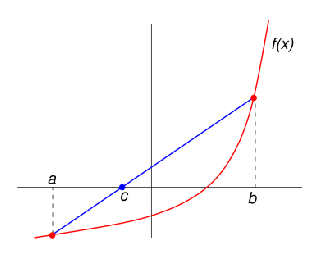
\epsfig{file=regula-falsi.eps,scale=1.0}
   \caption{Die Regula-Falsi zur Nullstellen-Bestimmung.}
  \label{fig:regula-falsi}
\end{figure}


Das Verfahren, dass mit dieser Formel arbeitet, ist unter dem Namen \emph{Regula Falsi}
bekannt und sieht genauso aus wie das Bisektions-Verfahren, nur dass wir f�r $c$ jetzt
die oben abgeleitete Formel verwenden:
\begin{enumerate}
\item[I.A.:] $n=0$.

      $a_0 := a$, \quad $b_0 := b$.
\item[I.S.:] $n \mapsto n+1$

      \hspace*{1.3cm} $c_n := \bruch{|f(b_n)|\cdot a_n + |f(a_n)|\cdot b_n}{|f(a_n)| + |f(b_n)|}$. \\[0.3cm]
      Dann definieren wir $a_{n+1}$ und $b_{n+1}$ durch Fall-Unterscheidung:
      \\[0.2cm]
      \hspace*{1.3cm}
      $\pair(a_{n+1},b_{n+1}) := 
         \left\{ \begin{array}{ll}
                 \pair(a_n,c_n) & \mbox{falls}\quad f(c_n) >    0 \\
                 \pair(c_n,b_n) & \mbox{falls}\quad f(c_n) \leq 0. \\
                 \end{array}
         \right.
      $
\end{enumerate}
�hnlich wie beim Beweis des Zwischenwert-Satzes l��t sich zeigen, dass die Folge
$\folge{a_n}$ monoton steigend ist, w�hrend die Folge $\folge{b_n}$ monoton fallend ist.
Da die Folgen �berdies beschr�nkt sind, denn $a_n$ ist immer kleiner als $b$ und $b_n$ ist
immer gr��er als $a$, konvergieren beide Folgen.  Allerdings ist nicht garantiert, dass
$a_n$ und $b_n$ gegen den gleichen Grenzwert konvergieren!  Es l��t sich lediglich zeigen,
dass entweder $a_n$ oder $b_n$ gegen eine Nullstelle der Funktion $f$ konvergiert.
Um das Verfahren experimentell untersuchen zu k�nnen, implementieren wir es.
Abbildung \ref{fig:regulaFalsi.stlx} zeigt die Implementierung der Methode
\textsl{findZero}().   Im Gegensatz zu der Implementierung des Bisektions-Verfahrens, in
dem wir nur gefordert hatten, dass die Funktion einen Vorzeichen-Wechsel in dem Intervall
$[a,b]$ hat, verlangen wir bei der Implementierung der Regula Falsi, dass
\\[0.2cm]
\hspace*{1.3cm}
$f(a) < 0$ \quad und \quad $f(b) > 0$ ist.
\\[0.2cm]
Diese Forderung erm�glicht eine etwas einfachere Implementierung.

Das letzte Argument der Methode \textsl{findZero}() gibt nun die gew�nschte Zahl der
Iterationen an.  Dieses Argument ist erforderlich, denn die Methode selber liefert uns
leider keinen Hinweis, wie gut die bisher berechnete N�herung ist.
Das liegt daran, dass im allgemeinen die Folgen $a_n$ und $b_n$ nicht gegen den selben
Grenzwert konvergieren.

Bei der R�ckgabe des berechneten Wertes in Zeile 16 ist es erforderlich, die Betr�ge der
Funktionswerte 
an den Intervall-Grenzen $a_n$ und $b_n$ zu vergleichen, denn wir wissen nicht, welche der
beiden Folgen gegen die Nullstelle konvergiert.  Wir geben daher als Ergebnis die
Intervall-Grenze  zur�ck, f�r die der Betrag des Funktionswertes am kleinsten ist.
Da wir wissen, dass der Funktionswert an der linken Intervall-Grenze immer kleiner als 0
ist, erhalten wir dort den Betrag indem wir dem Funktionswert das Minuszeichen vorstellen.

\begin{figure}[!ht]
  \centering
\begin{Verbatim}[ frame         = lines, 
                  framesep      = 0.3cm, 
                  labelposition = bottomline,
                  numbers       = left,
                  numbersep     = -0.2cm,
                  xleftmargin   = 0.5cm,
                  xrightmargin  = 0.5cm,
                ]
    regulaFalsi := procedure(f, a, b, n) {
        assert(a < b, "Error: !(a < b)");
        assert(f(a) < 0 && f(b) > 0, "Error: !(f(a) < 0 && f(b) > 0)");
        count := 0;
        fa := f(a); fb := f(b); 
        for (i in [1 .. n]) {
            c  := (fb * a - fa * b) / (fb - fa);
            fc := f(c); 
            if (fc <= 0) {
                a := c; fa := fc; 
            } else {
                b := c; fb := fc; 
            }
        }
        if (-fa < fb) {
            return a;
        } else {
            return b;
        }
    };
\end{Verbatim}
\vspace*{-0.3cm}
  \caption{Implementierung der Regula Falsi in \textsc{SetlX}.}
  \label{fig:regulaFalsi.stlx}
\end{figure} %\$

Tabelle \ref{tab:regula-falsi} zeigt die ersten 12 Iterations-Schritte, wenn die Regula Falsi
zur Berechnung der Nullstelle von $x  - \cos(x)$ eingesetzt wird.  Wir sehen,
dass wir bereits im 9-ten Schritt die selbe Genauigkeit erreicht haben, f�r die wir mit
dem Bisektions-Verfahren 30 Schritte ben�tigt haben.  Wir sehen auch, dass die rechte
Intervall-Grenze immer konstant bleibt.  Es sieht so aus, als ob wir mit der Regula Falsi
ein Verfahren haben, dass dem Bisektions-Verfahren �berlegen ist.  Die n�chste Aufgabe
zeigt Ihnen jedoch, dass dem Verfahren eine ganz wichtige Eigenschaft fehlt, die das
Bisektions-Verfahren besitzt:  Das Verfahren ist nicht robust!  Es gibt Funktionen, bei
denen die Regula Falsi zur Nullstellen-Bestimmung \textbf{\underline{wesentlich mehr}} Iterationen
ben�tigt als das Bisektions-Verfahren.
\vspace*{0.3cm}

\begin{table}[!h]
  \centering
\framebox{
  \begin{tabular}{|r|c|c|c|c|}
\hline
   $n$ & $a_n$ & $b_n$ & $f(a_n)$ & $f(b_n)$ \\
\hline
\hline
  1: & 0.000000000 & 1.000000000 & -1.00000000e+00 & 4.59697694e-01 \\ 
\hline
  2: & 0.685073357 & 1.000000000 & -8.92992765e-02 & 4.59697694e-01 \\ 
\hline
  3: & 0.736298997 & 1.000000000 & -4.66003904e-03 & 4.59697694e-01 \\ 
\hline
  4: & 0.738945356 & 1.000000000 & -2.33925666e-04 & 4.59697694e-01 \\ 
\hline
  5: & 0.739078130 & 1.000000000 & -1.17191742e-05 & 4.59697694e-01 \\ 
\hline
  6: & 0.739084782 & 1.000000000 & -5.87046549e-07 & 4.59697694e-01 \\ 
\hline
  7: & 0.739085115 & 1.000000000 & -2.94066726e-08 & 4.59697694e-01 \\ 
\hline
  8: & 0.739085132 & 1.000000000 & -1.47305551e-09 & 4.59697694e-01 \\ 
\hline
  9: & 0.739085133 & 1.000000000 & -7.37890543e-11 & 4.59697694e-01 \\ 
\hline
 10: & 0.739085133 & 1.000000000 & -3.69623245e-12 & 4.59697694e-01 \\ 
\hline
 11: & 0.739085133 & 1.000000000 & -1.85199566e-13 & 4.59697694e-01 \\ 
\hline
 12: & 0.739085133 & 1.000000000 & -9.23913723e-15 & 4.59697694e-01 \\ 
\hline
  \end{tabular}}
  \caption{Die ersten 12 Schritte der Regula Falsi zur L�sung von $x - \cos(x) = 0$.}
  \label{tab:regula-falsi}
\end{table}
\pagebreak

\exercise
 Verwenden Sie die Regula Falsi zur L�sung der Gleichung 
\\[0.2cm]
\hspace*{1.3cm}
$x^4 - 1 = 0$.
\\[0.2cm]
Starten Sie mit dem Intervall $[0, 10]$. Zeigen Sie, dass f�r alle nat�rlichen Zahlen $n$
mit $n \leq 1000$ die folgende Ungleichung f�r die linke Intervall-Grenze $a_n$ gilt:
\\[0.2cm]
\hspace*{1.3cm} $a_n \leq \bruch{n}{1000}$.
\\[0.2cm]
Die L�sung der Gleichung $x^4 - 1 = 0$ in dem Intervall ist $x=1$.  Aus der zu zeigenden
Ungleichung kann beispielsweise gefolgert werden, dass $a_{100} \leq 0.1$ gilt.  
 Der mit dem obigen Programm ermittelte Wert f�r $a_{100}$ ist
$a_{100} = 0.0985146583$.  In diesem Fall hat die Regula Falsi also selbst nach  100
Iterationen nicht eine einzige korrekte Stelle 
im Ergebnis berechnen k�nnen!  \eox
\vspace*{0.3cm}

\noindent
\textbf{L�sung}: Wir zeigen durch vollst�ndige Induktion �ber $n$, dass f�r alle 
$n\leq 1000$ zum einen die Ungleichung $a_n \leq n \cdot 10^{-3}$ gilt und dass zum anderen 
$b_n$ konstant ist, es gilt $b_n = 10$.
\begin{enumerate}
\item[I.A.:] $n = 0$.  Es gilt
      \\[0.2cm]
      \hspace*{1.3cm} $a_0 = 0 \leq 0 \cdot 10^{-3}$ \quad und \quad $b_0 = 10$.
\item[I.S.:] $n \mapsto n + 1$.

      Die Funktion $f := (x \mapsto x^4 - 1)$ ist f�r nichtnegative Zahlen monoton steigend,
      dass hei�t aus $0 \leq u \leq v$ folgt auch $f(u) \leq f(v)$.  Es gilt 
      \\[0.2cm]
      \hspace*{1.3cm}
      $f(n \cdot 10^{-3}) = n^4 \cdot 10^{-12} - 1$ \quad und \quad $f(10) = 10^4 - 1$.
      \\[0.2cm]
      Nach Induktions-Voraussetzung k�nnen wir $a_n$ durch $n\cdot 10^{-3}$ absch�tzen und 
      aufgrund der Monotonie von $f$ k�nnen wir dann $f(a_n)$ durch $f(n\cdot 10^{-3})$
      absch�tzen.
      Wenden wir daher f�r $a_n' = n \cdot 10^{-3}$ und $b_n=10$ die Regula Falsi an um eine
      N�herung $c_n'$ f�r die Nullstelle von $f$       zu berechnen, so wird
      $c_n'$ gr��er sein als der wahre Wert von $c_n$, der in dem Algorithmus tats�chlich auftritt.
      Es gilt:
      \\[0.2cm]
      \hspace*{1.3cm}
    $
    \begin{array}[t]{lcl}
    c_n' & = & \bruch{f(b_n) \cdot a_n' - f(a_n') \cdot b_n}{f(b_n) - f(a_n')} \\[0.5cm]
      & = & \bruch{f(10) \cdot n \cdot 10^{-3} + f\bigl(n\cdot 10^{-3}\bigr) \cdot 10}{f(10) - f\bigl(n\cdot 10^{-3}\bigr)} \\[0.5cm]
      & = & \bruch{\bigl(10^4 - 1\bigr) \cdot n \cdot 10^{-3} - \bigl(n^4 \cdot 10^{-12} - 1\bigr)\cdot 10}{10^4 - 1 - n^4\cdot 10^{-12} + 1} \\[0.5cm]
      & = & 10^{-4}\cdot \bruch{10 \cdot n - n \cdot 10^{-3} - n^4 \cdot 10^{-11} + 10}{1 - n^4\cdot 10^{-16}} \\[0.5cm]
      & = & 10^{-3}\cdot \bruch{n + 1 - n \cdot 10^{-4} - n^4 \cdot 10^{-12}}{1 - n^4\cdot 10^{-16}} \\[0.5cm]
    \end{array}  
    $
      \\[0.2cm]
      Wir untersuchen nun, f�r welche nat�rlichen Zahlen $n$ die Ungleichung 
      $c_n' \leq 10^{-3}\cdot (n+1)$ gilt.
      \\[0.2cm]
      \hspace*{1.3cm}
      $
      \begin{array}[t]{ll}        
                        & c_n' \leq 10^{-3}\cdot (n+1) \\[0.2cm]
        \Leftrightarrow & 10^{-3}\cdot \bruch{n + 1 - n \cdot 10^{-4} - n^4 \cdot 10^{-12}}{1 - n^4\cdot 10^{-16}} \leq 10^{-3}\cdot (n+1) \\[0.5cm]
        \Leftrightarrow & n + 1 - n \cdot 10^{-4} - n^4 \cdot 10^{-12} \leq (n+1)\cdot \bigl(1 - n^4\cdot 10^{-16}\bigr)   \\[0.3cm]
        \Leftrightarrow & n + 1 - n \cdot 10^{-4} - n^4 \cdot 10^{-12} \leq (n+1)  - (n+1)\cdot n^4\cdot 10^{-16}   \\[0.3cm]
        \Leftrightarrow & - n \cdot 10^{-4} - n^4 \cdot 10^{-12} \leq   - (n+1)\cdot n^4\cdot 10^{-16}   \\[0.3cm]
        \Leftrightarrow & n \cdot 10^{-4} + n^4 \cdot 10^{-12} \geq  (n+1)\cdot n^4\cdot 10^{-16}   \\[0.3cm]
        \Leftarrow      & n^4 \cdot 10^{-12} \geq  (n+1)\cdot n^4\cdot 10^{-16}   \\[0.3cm]
        \Leftrightarrow & 1 \geq  (n+1)\cdot 10^{-4}   \\[0.3cm]
        \Leftrightarrow & 10^4 \geq  n+1   \\[0.3cm]
        \Leftrightarrow & n \leq 9999   
      \end{array}
      $
      \\[0.3cm]
      Solange $n < 1000$ ist, gilt also sicher $c_n' < 1$ und damit ist $f(c_n')$ negativ.
      Daher gilt 
      \\[0.2cm]
      \hspace*{1.3cm}  $a_{n+1} \leq a_{n+1}' = c_n' \leq 10^{-3} \cdot n$ und $b_{n+1} = b_n = 1$.
      \qed
\end{enumerate}

\subsection{Das Sekanten-Verfahren}
Ein Problem bei der Regula Falsi scheint darin zu liegen, dass h�ufig eine
Intervall-Grenze w�hrend der gesamten Iteration fest bleibt.  Dies war schon bei der
Bestimmung der Nullstelle der Funktion $x \mapsto x - \cos(x)$ der Fall.  Eine
M�glichkeit, dieses Problem zu umgehen besteht darin, dass wir anstatt eine Folge von
Intervallen $\folge{[a_n, b_n]}$ zu bilden einfach nur eine Folge von Punkten
$\folge{x_n}$ bilden.  Den Punkt $x_{n+1}$ bestimmen wir, indem wir durch die Punkte
$x_{n+1}$ und $x_n$ eine Gerade legen und dann $x_n$ als den Schnittpunkt dieser Geraden
mit der $x$-Achse bestimmen.  Das f�hrt auf die selbe Formel wie bei der Regula-Falsi, wir
setzen n�mlich
\\[0.2cm]
\hspace*{1.3cm}
$x_{n+1} := \bruch{f(x_{n}) \cdot x_{n-1} - f(x_{n-1}) \cdot x_n}{f(x_{n}) - f(x_{n-1})}$.
\\[0.2cm]
Dann brauchen wir nur noch zwei Startwerte $x_0$ und $x_1$ und die Rechnung kann los gehen.
Abbildung \ref{fig:secant.stlx} zeigt eine Implementierung des Sekanten-Verfahrens in
\textsc{SetlX}.  Testen wir dieses Programm mit der Funktion $x \mapsto x - \cos(x)$, so
erhalten wir die in Tabelle \ref{tab:secant-method} gezeigten Werte.
Wir sehen, dass jetzt bereits 7 Iterationen ausreichen, um die L�sung der Gleichung mit
der geforderten Genauigkeit zu berechnen.  Es sieht also so aus, als ob das
Sekanten-Verfahren den anderen Verfahren �berlegen ist.  In der Tat kann gezeigt werden, dass
das Sekanten-Verfahren, \textbf{wenn} es denn konvergiert, schneller konvergiert als die anderen
Verfahren. Wir werden das sp�ter pr�zisieren.  Das Problem ist, dass das Sekanten-Verfahren
gar nicht immer konvergiert.  Betrachten wir beispielsweise die Funktion 
\\[0.2cm]
\hspace*{1.3cm}
$x \mapsto \bruch{2}{x^2 + 1} - 1$. 
\\[0.2cm]
Diese Funktion hat bei $x = 1.0$ eine Nullstelle.  Mit
den Startwerten $a = 0$ und $b = 5.0$ produziert unser Programm die in Tabelle
\ref{tab:secant-method2}
gezeigten Werte.


\begin{figure}[!ht]
  \centering
\begin{Verbatim}[ frame         = lines, 
                  framesep      = 0.3cm, 
                  labelposition = bottomline,
                  numbers       = left,
                  numbersep     = -0.2cm,
                  xleftmargin   = 0.5cm,
                  xrightmargin  = 0.5cm,
                ]
    secant := procedure(f, a, b, digits) {
        fa := f(a); 
        fb := f(b); 
        while (abs(b - a) > (1/10)**(digits + 1)) {
            c := (fb * a - fa * b) / (fb - fa);
            a := b; b := c; fa := fb; fb := f(c); 
        }
        return b;
    };
\end{Verbatim}
\vspace*{-0.3cm}
  \caption{Implementierung des Sekanten-Verfahrens in \textsc{SetlX}.}
  \label{fig:secant.stlx}
\end{figure} %\$


\begin{table}[!h]
  \centering
\framebox{
  \begin{tabular}{|r|r|r|}
\hline
   $n$ & $x_n$ & $f(x_n)$ \\
\hline
\hline
  1: & \texttt{10.00000000000} & \texttt{+1.08390715e+01} \\
\hline
  2: & \texttt{ 0.84466083134} & \texttt{+1.80675899e-01} \\
\hline
  3: & \texttt{ 0.68946400911} & \texttt{-8.21230732e-02} \\
\hline
  4: & \texttt{ 0.73796206792} & \texttt{-1.87910933e-03} \\
\hline
  5: & \texttt{ 0.73909776898} & \texttt{+2.11474296e-05} \\
\hline
  6: & \texttt{ 0.73908513008} & \texttt{-5.24715686e-09} \\
\hline
  7: & \texttt{ 0.73908513322} & \texttt{-1.46275678e-14} \\
\hline
  \end{tabular}}
  \caption{L�sung der Gleichung $x - \cos(x) = 0$ mit dem Sekanten-Verfahren.}
  \label{tab:secant-method}
\end{table}



\begin{table}[!h]
  \centering
\framebox{
  \begin{tabular}{|r|r|r|}
\hline
   $n$ & $x_n$ & $f(x_n)$ \\
\hline
\hline
  1: & \texttt{+5.000000e+00} & \texttt{-0.923076923} \\
\hline
  2: & \texttt{+2.600000e+00} & \texttt{-0.742268041} \\
\hline
  3: & \texttt{-7.252631e+00} & \texttt{-0.962687030} \\
\hline
  4: & \texttt{+3.577905e+01} & \texttt{-0.998438891}\\
\hline
  5: & \texttt{-1.165962e+03} & \texttt{-0.999998529}\\
\hline
  6: & \texttt{+7.693592e+05} & \texttt{-1.000000000}\\
\hline
  7: & \texttt{-5.237534e+11} & \texttt{-1.000000000}\\
\hline
  8: & \texttt{+1.550094e+23} & \texttt{-1.000000000}\\
\hline
  9: & $\infty$               & \texttt{-1.000000000}\\
\hline
  \end{tabular}}
  \caption{Divergenz des Sekanten-Verfahrens bei der L�sung von $\bruch{2}{x^2 + 1} - 1 = 0$.}
  \label{tab:secant-method2}
\end{table}

\pagebreak
\vspace*{\fill}

\pagebreak

\subsection{Das Illinois-Verfahren}
Von den bisher vorgestellten Verfahren ist nur das Bisektions-Verfahren wirklich robust.
Bei der Regula-Falsi ist das Problem, dass eine Intervall-Grenze stehen bleiben kann. Am
Beispiel der Funktion $x \mapsto x^4 - 1$ haben wir gesehen, dass dies zu einer sehr
langsamen Konvergenz f�hren kann.  Beim Sekanten-Verfahren hatten wir dieses Problem
behoben, aber dort kann es in ung�nstigen F�llen passieren, dass das Verfahren �berhaupt nicht mehr
konvergiert.  Das \emph{Illinois-Verfahren} \cite{dowell:1971} versucht die Konvergenz der Regula Falsi
auf andere Weise zu beschleunigen.  Die Idee des Verfahrens ist eigentlich sehr naheliegend:
Wenn bei der Regula Falsi eine der Intervall-Grenzen �ber zwei oder mehr Schritte konstant bleibt,
dann wird der Funktionswert an der betreffenden Intervall-Grenze halbiert, so dass der Einfluss dieses
Wertes bei der Berechnung der n�chsten N�herung $c_n$ nach der Formel
\\[0.2cm]
\hspace*{1.3cm}
$c_n := \bruch{f(b_n) \cdot a_n - f(a_n) \cdot b_n}{f(b_n) - f(a_n)}$
\\[0.2cm]
gemindert wird.  Nehmen wir o.B.d.A.~an, dass $f(a) < 0$ und $0 < f(b)$ ist, so f�hrt das zur folgenden 
Definition der Folgen $\folge{a_n}$ und $\folge{b_n}$:
\begin{enumerate}
\item[I.A.:] $n=0$.  Wir setzen 
             \\[0.2cm]
             \hspace*{1.3cm}
             $a_0 := a$, \quad $b_0 := b$, \quad $\alpha_0 := 1$, \quad und \quad $\beta_0 := 1$.
             \\[0.2cm]
             Die Werte $\alpha_n$ und $\beta_n$ sind dabei Gewichtungs-Faktoren, die wir sp�ter ben�tigen.
\item[I.S.:] $n \mapsto n+1$.  Wir definieren �hnlich wie bei der Regula Falsi den Wert $c_n$ als \\[0.2cm]
      \hspace*{1.3cm} 
      $c_n := \bruch{\beta_n \cdot f(b_n) \cdot a_n - \alpha_n \cdot f(a_n) \cdot b_n}{
                     \beta_n \cdot f(b_n) - \alpha_n \cdot f(a_n)}
      $. 
      \\[0.3cm]
      Der Unterschied zur Regula Falsi liegt in den Gewichtungs-Faktoren $\alpha_n$ und $\beta_n$.
      Die Werte f�r $a_{n+1}$ und $b_{n+1}$ werden durch die selbe Fall-Unterscheidung wie bei der Regula
      Falsi festgelegt:
      \\[0.2cm]
      \hspace*{1.3cm}
      $\pair(a_{n+1},b_{n+1}) := 
         \left\{ \begin{array}{ll}
                 \pair(a_n,c_n) & \mbox{falls}\quad f(c_n) >    0 \\
                 \pair(c_n,b_n) & \mbox{falls}\quad f(c_n) \leq 0. \\
                 \end{array}
         \right.
      $
      \\[0.2cm]
      Falls wir nun feststellen, dass $b_{n+1} = b_{n-1}$ ist, so hat sich der Wert der rechten
      Intervall-Grenze w�hrend der letzten zwei Iterationen nicht ge�ndert.  Wir wollen diesen Wert
      daher beim n�chsten Iterations-Schritt 
      schw�cher gewichten und setzen deshalb in diesem Fall
      \\[0.2cm]
      \hspace*{1.3cm}
      $\beta_{n+1} = \bruch{1}{2} \cdot \beta_n$ \quad und \quad $\alpha_{n+1} := 1$.
      \\[0.2cm]
      Ist umgekehrt $a_{n+1} = a_{n-1}$, so hat sich der Wert der linken
      Intervall-Grenze nicht ge�ndert.  Wir gewichten daher die linke Intervall-Grenze beim n�chsten
      Iterations-Schritt schw�cher und setzen 
      \\[0.2cm]
      \hspace*{1.3cm}
      $\beta_{n+1} = 1$ \quad und \quad $\alpha_{n+1} := \bruch{1}{2} \cdot \alpha_n$.
\end{enumerate}
Die Umsetzung dieses Verfahrens sehen Sie in Abbildung \ref{fig:illinois.stlx}.  In den Variablen
\texttt{oldA1} und \texttt{oldB1} speichern wir die Werte von $a_{n-1}$ und $b_{n-1}$, in den
Variablen \texttt{oldA2} und \texttt{oldB2} sind die Werte $a_{n-2}$ und $b_{n-2}$ gespeichert.  Wir
initialisieren diese Werte mit $\mathtt{om}$, denn $\mathtt{om}$ bezeichnet in \textsc{SetlX}
den undefinierten Wert.
Falls wir in Zeile 19 feststellen, dass der Wert von $a_n = a_{n-2}$ ist, dann setzen wir den Wert
$\alpha_{n+1}$ auf $\alpha_n/2$.  Analog testen wir in Zeile 14, ob $b_n = b_{n-2}$ ist und setzen
gegebenenfalls $\beta_{n+1}$ auf $\beta_n/2$.



\begin{figure}[!ht]
  \centering
\begin{Verbatim}[ frame         = lines, 
                  framesep      = 0.3cm, 
                  labelposition = bottomline,
                  numbers       = left,
                  numbersep     = -0.2cm,
                  xleftmargin   = 0.0cm,
                  xrightmargin  = 0.0cm,
                ]
    illinois := procedure(f, a, b, n) {
        assert(a < b, "a has to be less than b");
        [ fa, fb ] := [ f(a), f(b) ];
        assert(fa < 0 && 0 < fb, "We need f(a) < 0 and 0 < f(b)!");
        k := 1;
        oldA1 := om; oldB1 := om;
        oldA2 := om; oldB2 := om;
        alpha := 1; beta := 1;
        while (k <= n) {
            c  := (beta * fb * a - alpha * fa * b) / (beta * fb - alpha * fa);
            fc := f(c);
            if (fc < 0) {
                a := c; fa := fc; alpha := 1;
                if (oldB2 == b) {
                    beta /= 2;
                }
            } else if (fc > 0) {
                b := c; fb := fc; beta := 1;
                if (oldA2 == a) {
                    alpha /= 2;
                }
            } else {
                return c;
            }
            oldA2 := oldA1; oldB2 := oldB1;
            oldA1 := a;     oldB1 := b;
        }
        return (a + b) / 2;
    };
\end{Verbatim}
\vspace*{-0.3cm}
  \caption{Implementierung des Illinois-Verfahrens zur Berechnung von Nullstellen.}
  \label{fig:illinois.stlx}
\end{figure} 
\pagebreak

\section{Differenzierbare Funktionen}
Wir haben nun alles Material zusammen, um den Begriff der \emph{Ableitung} definieren zu k�nnen, welcher
der wichtigste Begriff der Analysis ist.  Dieser Begriff wurde unabh�ngig von 
\href{http://de.wikipedia.org/wiki/Isaac_Newton}{Isaac Newton} und
\href{http://de.wikipedia.org/wiki/Gottfried_Wilhelm_Leibniz}{Gottfried Wilhelm Leibniz} gefunden,
die folgende formale Definition der Ableitung geht auf 
\href{http://de.wikipedia.org/wiki/Augustin-Louis_Cauchy}{Augustin-Louis Cauchy} zur�ck.

\begin{Definition}[Ableitung]
Eine Funktion $f: D \rightarrow \mathbb{R}$ ist im Punkt $\widehat{x} \in D$ \emph{differenzierbar},
wenn der Grenzwert
\\[0.3cm]
\hspace*{1.3cm}
$\lim\limits_{h \rightarrow 0} \bruch{f(\widehat{x} + h) - f(\widehat{x})}{h}$
\\[0.3cm]
existiert.  In diesem Fall definieren wir 
\\[0.3cm]
\hspace*{1.3cm}
$\displaystyle\frac{d\,f}{dx}(\widehat{x}) = \lim\limits_{h \rightarrow 0}
\bruch{f(\widehat{x} + h) - f(\widehat{x})}{h}$.
\\[0.3cm]
Wir bezeichnen den Wert $\ds\frac{d\,f}{dx}(\widehat{x})$ als die \emph{Ableitung} der
Funktion $f$ an der Stelle $\widehat{x}$.  Gelegentlich werden \\[0.2cm]
wir f�r die Ableitung auch die Schreibweise 
$f'(\widehat{x})$ verwenden.
\eod
\end{Definition}


\remark
Beachten Sie, dass wir in der obigen Definition den Ausdruck
\\[0.3cm]
\hspace*{1.3cm} $\bruch{f(\widehat{x} + h) - f(\widehat{x})}{h}$ \\[0.3cm]
als Funktion von $h$ auffassen.  Dieser Ausdruck wird auch als \emph{Differential-Quotient}
bezeichnet.  Er gibt die Steigung einer Sekante an, die die Funktion $x \mapsto f(x)$
in den Punkten $\widehat{x}$ und $\widehat{x} + h$ schneidet.  Definieren wir 
\\[0.3cm]
\hspace*{1.3cm}
$r(h) := f(\widehat{x} + h) - f(\widehat{x}) - h \cdot \df{f}(\widehat{x})$,
\\[0.3cm]
so gilt einerseits 
\\[0.3cm]
\hspace*{1.3cm}
$\lim\limits_{h \rightarrow 0} \bruch{r(h)}{h} = 
 \lim\limits_{h \rightarrow 0} \bruch{f(\widehat{x} + h) -
  f(\widehat{x})}{h} - \df{f}(\widehat{x}) = \df{f}(\widehat{x}) - \df{f}(\widehat{x}) = 0$,
\\[0.3cm]
und andererseits haben wir 
\\[0.3cm]
\hspace*{1.3cm}
$f(\widehat{x} + h) = f(\widehat{x}) + h \cdot \df{f}(\widehat{x}) + r(h)$.
\\[0.3cm]
Die Funktion $r(h)$ ist also der Fehler, der bei der linearen Approximation
entsteht.  \eox


\remark
Falls die Funktion $f$ im Punkt $\widehat{x}$ differenzierbar ist,
dann ist die Funktion dort auch stetig, denn es gilt 
\\[0.3cm]
\hspace*{1.3cm}
$
\begin{array}[t]{lcl}
\lim\limits_{h \rightarrow 0} f(\widehat{x}+h) & = &
 \lim\limits_{h \rightarrow 0} f(\widehat{x}+h) - f(\widehat{x}) + f(\widehat{x}) \\[0.3cm]
& = & \lim\limits_{h \rightarrow 0} \bruch{f(\widehat{x}+h) - f(\widehat{x})}{h} \cdot h + f(\widehat{x}) \\[0.3cm]
& = & \lim\limits_{h \rightarrow 0} \bruch{f(\widehat{x}+h) - f(\widehat{x})}{h} \cdot \lim\limits_{h \rightarrow 0} h + f(\widehat{x}) \\[0.3cm]
& = & f'(\widehat{x}) \cdot 0 + f(\widehat{x}) \\[0.3cm]
& = & f(\widehat{x})
\end{array}
$
\\[0.3cm]
und $\lim\limits_{h \rightarrow 0} f(\widehat{x}+h) = f(\widehat{x})$ hei�t gerade, dass $f$
im Punkt $\widehat{x}$ stetig ist. \qed
\vspace*{0.3cm}

\examples
\begin{enumerate}
\item Die konstante Funktion $f := (x \mapsto c)$ hat �berall die Ableitung
      $0$, denn es gilt \\[0.3cm]
      \hspace*{1.3cm}$\lim\limits_{h \rightarrow 0} \bruch{f(\widehat{x} + h) - f(\widehat{x})}{h} =
\lim\limits_{h \rightarrow 0} \bruch{c - c}{h} = \lim\limits_{h \rightarrow 0} 0 = 0$.
\item Die identische Funktion $\textsl{id} := (x \mapsto x)$ hat �berall die Ableitung 1,
      denn es gilt: 
      \\[0.3cm]
      \hspace*{1.3cm}
      $\lim\limits_{h \rightarrow 0} \bruch{\textsl{id}(\widehat{x} + h) - \textsl{id}(\widehat{x})}{h} =
       \lim\limits_{h \rightarrow 0} \bruch{\widehat{x} + h - \widehat{x}}{h} =
       \lim\limits_{h \rightarrow 0} \bruch{h}{h} = \lim\limits_{h \rightarrow 0} 1 = 1$.
\item Die Funktion $\textsl{abs} := ( x \mapsto |x|)$, die den Absolutbetrag berechnet, ist im
      Punkte $\widehat{x} = 0$ nicht differenzierbar.  Wir zeigen, dass der Grenzwert
      \\[0.3cm]
      \hspace*{1.3cm}
            $\lim\limits_{h \rightarrow 0} \bruch{\textsl{abs}(h) - \textsl{abs}(0)}{h}$
      \\[0.3cm]
      nicht existiert.  Dazu betrachten wir zun�chst die Folge $\folge{\frac{1}{n}}$.
      Nehmen wir an, dass dieser Grenzwert existiert und den Wert $a$ hat.  
      Da \\[0.3cm]
      \hspace*{1.3cm}
      $\lim\limits_{n\rightarrow\infty} \frac{1}{n} = 0$ 
      \\[0.3cm]
      ist, m��te nach Definition des Grenzwerts dann gelten: \\[0.3cm]
      \hspace*{1.3cm}
      $a = \displaystyle \lim\limits_{h \rightarrow 0} \bruch{\textsl{abs}(h) - \textsl{abs}(0)}{h} = 
       \lim\limits_{n\rightarrow\infty} \frac{\textsl{abs}(\frac{1}{n})}{\frac{1}{n}} = 
       \lim\limits_{n\rightarrow\infty} \frac{\;\frac{1}{n}\;}{\frac{1}{n}} = 1 $.
      \\[0.3cm]
      Betrachten wir andererseits die Folge $\folge{-\frac{1}{n}}$ und ber�cksichtigen,
      dass diese Folge ebenfalls gegen 0 konvergiert, so erhalten wir
      \\[0.3cm]
      \hspace*{1.3cm}
      $a = \displaystyle \lim\limits_{h \rightarrow 0} \bruch{\textsl{abs}(h) - \textsl{abs}(0)}{h} = 
       \lim\limits_{n\rightarrow\infty} \frac{\textsl{abs}(-\frac{1}{n})}{-\frac{1}{n}} = 
       \lim\limits_{n\rightarrow\infty} \frac{\;\frac{1}{n}\;}{-\frac{1}{n}} = -1$.
      \\[0.3cm]
      Da $a$ nicht gleichzeitig die Werte $+1$ und $-1$ annehmen kann, m�ssen wir folgern,
      dass die Funktion $\textsl{abs}$ an der Stelle $\widehat{x} = 0$ nicht
      differenzierbar ist.  \eox
\end{enumerate}


\begin{Satz}[Ableitungs-Regeln]
Es seien $f: D \rightarrow \mathbb{R}$  und $g: D \rightarrow \mathbb{R}$ Funktionen, die
im Punkt $\widehat{x}$ differenzierbar sind. Dann gilt:
\begin{enumerate}
\item Die Funktion $f + g := \bigl(x \mapsto f(x) + g(x)\bigr)$ ist im Punkt $\widehat{x}$
      differenzierbar und es gilt:
      \\[0.3cm]
      \hspace*{1.3cm} $(f+ g)'(\widehat{x}) = f'(\widehat{x}) + g'(\widehat{x})$.
\item Die Funktion $f - g := \bigl(x \mapsto f(x) - g(x)\bigr)$ ist im Punkt $\widehat{x}$
      differenzierbar und es gilt:
      \\[0.3cm]
      \hspace*{1.3cm} $(f - g)'(\widehat{x}) = f'(\widehat{x}) - g'(\widehat{x})$.
\item Die Funktion $f \cdot g := \bigl(x \mapsto f(x) \cdot g(x)\bigr)$ ist im Punkt $\widehat{x}$
      differenzierbar und es gilt die Produkt-Regel:
      \\[0.3cm]
      \hspace*{1.3cm} $(f \cdot g)'(\widehat{x}) = f'(\widehat{x})\cdot g(\widehat{x}) + f(\widehat{x})\cdot g'(\widehat{x})$.
\item Ist $g(\widehat{x}) \not= 0$, dann ist
      die Funktion $\bruch{f}{g} := \Bigl(x \mapsto \bruch{f(x)}{g(x)}\Bigr)$ im Punkt $\widehat{x}$
      differenzierbar und es gilt die Quotienten-Regel:
      \\[0.3cm]
      \hspace*{1.3cm} $\left(\bruch{f}{g}\right)'(\widehat{x}) = \bruch{f'(\widehat{x})\cdot g(\widehat{x}) - f(\widehat{x})\cdot g'(\widehat{x})}{g(\widehat{x})^2}$.
\end{enumerate}
\end{Satz}

\noindent
\textbf{Beweis}: Wir zeigen nur die Produkt-Regel.  Es gilt:
\\[0.3cm]
\hspace*{0.3cm}
$
\begin{array}[t]{lcl}
 &   &  (f \cdot g)'(\widehat{x}) \\[0.2cm]
 & = & \lim\limits_{h \rightarrow 0} \bruch{(f\cdot g)(\widehat{x} + h) - (f\cdot g)(\widehat{x})}{h} \\[0.3cm]
 & = &  \lim\limits_{h \rightarrow 0} \bruch{f(\widehat{x} + h)\cdot g(\widehat{x} + h) - f(\widehat{x})\cdot g(\widehat{x})}{h} \\[0.3cm]
 & = &  \lim\limits_{h \rightarrow 0} \bruch{f(\widehat{x} + h)\cdot g(\widehat{x} + h) - f(\widehat{x})\cdot g(\widehat{x} + h)}{h} + 
                                      \bruch{f(\widehat{x})\cdot g(\widehat{x} + h) - f(\widehat{x})\cdot g(\widehat{x})}{h} \\[0.3cm]
 & = &  \lim\limits_{h \rightarrow 0} \bruch{f(\widehat{x} + h)\cdot g(\widehat{x} + h) - f(\widehat{x})\cdot g(\widehat{x} + h)}{h} +
        \lim\limits_{h \rightarrow 0} \bruch{f(\widehat{x})\cdot g(\widehat{x} + h) - f(\widehat{x})\cdot g(\widehat{x})}{h} \\[0.3cm]
 & = &  \lim\limits_{h \rightarrow 0} \bruch{f(\widehat{x} + h) - f(\widehat{x})}{h} \cdot \lim\limits_{h \rightarrow 0} g(\widehat{x}+h) +
        \lim\limits_{h \rightarrow 0} f(\widehat{x}) \cdot \lim\limits_{h \rightarrow 0} \bruch{g(\widehat{x} + h) - g(\widehat{x})}{h} \\[0.4cm]
 & = &  f'(\widehat{x}) \cdot  g(\widehat{x}) + f(\widehat{x}) \cdot g'(\widehat{x}) \\[0.3cm]
\end{array}
$
\\[0.3cm]
Dabei haben wir im letzten Schritt ausgenutzt, dass eine differenzierbare Funktion auch stetig ist.
Daher gilt 
\\[0.2cm]
\hspace*{1.3cm}
$\lim\limits_{h \rightarrow 0} g(\widehat{x} + h) = g(\widehat{x})$. \hspace*{\fill} $\Box$
\vspace*{0.3cm}

\exercise
Zeigen Sie: Ist die Funktion $g$ im Punkt $\widehat{x}$ differenzierbar und gilt
$g(\widehat{x}) \not= 0$, so ist auch die Funktion 
$\bruch{1}{g} := \left(x \mapsto \bruch{1}{g(x)}\right)$ im Punkt $\widehat{x}$
differenzierbar und es gilt 
\\[0.3cm]
\hspace*{1.3cm} 
$\left(\bruch{1}{g}\right)'(\widehat{x}) = -\bruch{g'(\widehat{x})}{g(\widehat{x})^2}$.
\\[0.3cm]
Folgern Sie aus diesem Ergebnis die Quotienten-Regel.
\eox

\begin{Satz}[Ketten-Regel] 
  Die Funktionen $f:\mathbb{R} \rightarrow \mathbb{R}$ 
  sei differenzierbar im Punkt $\widehat{x}\in\mathbb{R}$ und die Funktion
  $g:\mathbb{R} \rightarrow \mathbb{R}$ sei differenzierbar im Punkt 
  $\widehat{y} = f(\widehat{x})$.  Dann ist auch die Funktion
  \\[0.2cm]
  \hspace*{1.3cm}
  $g \circ f := \bigr(x \mapsto g(f(x))\bigr)$ 
  \\[0.2cm]
  im Punkt $\widehat{x}$  differenzierbar und es gilt 
  \\[0.3cm]
  \hspace*{1.3cm}
  $(g\circ f)'(\widehat{x}) = g'(f(\widehat{x})) \cdot f'(\widehat{x})$.  
\end{Satz}

\noindent
\textbf{Beweis}: 
Aus der Differenzierbarkeit von $f$ und $g$ folgt, dass es Funktionen $r_1(h)$ und
$r_2(h)$ gibt, so dass gilt:
\begin{enumerate}
\item $f(\widehat{x}+h) = f(\widehat{x}) + h\cdot f'(\widehat{x}) + r_1(h)$ \quad mit $\lim\limits_{h \rightarrow 0} \bruch{r_1(h)}{h} = 0$,
\item $g(\widehat{y}+h) = g(\widehat{y}) + h\cdot g'(\widehat{y}) + r_2(h)$ \quad mit $\lim\limits_{h \rightarrow 0} \bruch{r_2(h)}{h} = 0$.
\end{enumerate}
Damit finden wir f�r den Differential-Quotienten der Funktion $g \circ f$ im Punkt
$\widehat{x}$: \\[0.3cm]
\hspace*{1.3cm}
$
\begin{array}[t]{lcl}
& & \bruch{(g\circ f)(\widehat{x} + h) - (g\circ f)(\widehat{x})}{h} \\[0.3cm]
&=& \bruch{g\bigl(f(\widehat{x} + h)\bigr) - g\bigl(f(\widehat{x})\bigr)}{h} \\[0.3cm]
&=& \bruch{g\bigl(f(\widehat{x}) + h\cdot f'(\widehat{x}) + r_1(h)\bigr) - g\bigl(f(\widehat{x})\bigr)}{h} \\[0.3cm]
&=& \bruch{g\bigl(\widehat{y} + h\cdot f'(\widehat{x}) + r_1(h)\bigr) - g\bigl(\widehat{y}\bigr)}{h} \\[0.3cm]
&=& \bruch{g(\widehat{y}) + \bigl(h\cdot f'(\widehat{x}) + r_1(h)\bigr)\cdot g'(\widehat{y}) + r_2\bigl(h\cdot f'(\widehat{x}) + r_1(h)\bigr) - g(\widehat{y})}{h} \\[0.3cm]
&=& f'(\widehat{x})\cdot g'(\widehat{y}) + \bruch{r_1(h)}{h}\cdot g'(\widehat{y}) + \bruch{r_2\bigl(h\cdot f'(\widehat{x}) + r_1(h)\bigr)}{h} \\[0.3cm]
\end{array}
$
\\[0.3cm]
Wenn wir jetzt den Grenzwert $h \rightarrow 0$ berechnen, dann m�ssen wir uns den letzten
Term genauer ansehen. Es gilt 
\\[0.3cm] 
\hspace*{1.3cm}
 $
 \begin{array}[t]{lcl}
 \lim\limits_{h \rightarrow 0}\bruch{r_2\bigl(h\cdot f'(\widehat{x}) + r_1(h)\bigr)}{h} &=&
 \lim\limits_{h \rightarrow 0}\bruch{r_2\bigl(h\cdot f'(\widehat{x}) + r_1(h)\bigr)}{h\cdot f'(\widehat{x}) + r_1(h)} \cdot \bruch{h\cdot f'(\widehat{x}) + r_1(h)}{h} \\[0.5cm]
& = & \lim\limits_{h \rightarrow 0}\bruch{r_2\bigl(h\cdot f'(\widehat{x}) + r_1(h)\bigr)}{h\cdot f'(\widehat{x}) + r_1(h)} \cdot 
      \lim\limits_{h \rightarrow 0} \bruch{h\cdot f'(\widehat{x}) + r_1(h)}{h} \\[0.5cm]
& = & \lim\limits_{h \rightarrow 0}\bruch{r_2\bigl(h\bigr)}{h} \cdot 
      \left(\lim\limits_{h \rightarrow 0} f'(\widehat{x}) + \bruch{r_1(h)}{h}\right) \\[0.5cm]
& = & 0 \cdot \bigl(f'(\widehat{x}) + 0\bigr) \\[0.2cm]
& = & 0
\end{array}
$
\\[0.3cm]
Damit sehen wir:
\\[0.3cm]
\hspace*{1.3cm}
$
\begin{array}[t]{lcl}
 & & \lim\limits_{h \rightarrow 0} \bruch{(g\circ f)(\widehat{x} + h) - (g\circ f)(\widehat{x})}{h} \\[0.5cm]
 & = & \lim\limits_{h \rightarrow 0} f'(\widehat{x})\cdot g'(\widehat{y}) + \bruch{r_1(h)}{h}\cdot g'(\widehat{y}) + \bruch{r_2\bigl(h\cdot f'(\widehat{x}) + r_1(h)\bigr)}{h} \\[0.5cm]
 &=& f'(\widehat{x})\cdot g'(\widehat{y}) + \lim\limits_{h \rightarrow 0} \bruch{r_1(h)}{h}\cdot g'(\widehat{y}) + \lim\limits_{h \rightarrow 0} \bruch{r_2\bigl(h\cdot f'(\widehat{x}) + r_1(h)\bigr)}{h} \\[0.5cm]
 &=& f'(\widehat{x})\cdot g'(\widehat{y}) + 0 + 0 \\[0.3cm]
 &=& f'(\widehat{x})\cdot g'(\widehat{y}).
\end{array}
$
\\[0.3cm]
Der obige exakte Beweis ist recht umst�ndlich.  Wir geben daher zus�tzlich eine
Plausibilit�tsbetrachtung.  Nach Definition der Ableitung gilt 
\\[0.3cm]
\hspace*{1.3cm}
$g'(\widehat{y}) = \lim\limits_{h \rightarrow 0} \bruch{g(\widehat{y} + h) - g(\widehat{y})}{h}$
\\[0.3cm]
F�r kleine Werte von $h$ gilt daher ungef�hr 
\\[0.2cm]
\hspace*{1.3cm}
$g(\widehat{y} + h) \approx g(\widehat{y}) + g'(\widehat{y})\cdot h$.
\\[0.2cm]
Analog finden wir f�r die Funktion $f$
\\[0.2cm]
\hspace*{1.3cm}
$f(\widehat{x} + h) \approx f(\widehat{x}) + f'(\widehat{x})\cdot h$.
\\[0.2cm]
Damit finden wir f�r den Differential-Quotienten der Funktion $g \circ f$ im Punkt
$\widehat{x}$: \\[0.3cm]
\hspace*{1.3cm}
$
\begin{array}[t]{lcl}
 \bruch{(g\circ f)(\widehat{x} + h) - (g\circ f)(\widehat{x})}{h} 
&=& \bruch{g\bigl(f(\widehat{x} + h)\bigr) - g\bigl(f(\widehat{x})\bigr)}{h} \\[0.3cm]
&\approx& \bruch{g\bigl(f(\widehat{x}) + f'(\widehat{x})\cdot h\bigr) - g\bigl(f(\widehat{x})\bigr)}{h} \\[0.3cm]
&\approx& \bruch{g\bigl(f(\widehat{x})\bigr) + g'\bigl(f(\widehat{x})\bigr)\cdot f'(\widehat{x})\cdot h - g\bigl(f(\widehat{x})\bigr)}{h} \\[0.3cm]
&=& \bruch{g'\bigl(f(\widehat{x})\bigr)\cdot f'(\widehat{x})\cdot h}{h} \\[0.3cm]
&=& g'\bigl(f(\widehat{x})\bigr)\cdot f'(\widehat{x}) \\[0.3cm]
\end{array}
$
\\[0.3cm]
Die linke Seite der Gleichung stellt den Differential-Quotienten der Funktion $g\circ f$
dar und mu� daher f�r $h \rightarrow 0$ gegen die Ableitung $(g \circ f)(\widehat{x})$
konvergieren. \hspace*{\fill} $\Box$
\pagebreak

\exercise
 Zeigen Sie, dass f�r alle nat�rlichen Zahlen $n$ gilt: 
\\[0.3cm]
\hspace*{1.3cm}
$\displaystyle\frac{d\,x^n}{dx} = n \cdot x^{n-1}$.


\begin{Satz}[Ableitung von Potenzreihen]
Ist die Funktion $f$ als Potenzreihe definiert, 
\\[0.3cm]
\hspace*{1.3cm} $\sum\limits_{n=0}^\infty a_n \cdot  x^n$ 
\\[0.3cm]
und ist $R$ der Konvergenz-Radius dieser Potenzreihe, so ist $f$ f�r alle $x\in\mathbb{R}$
mit $|x| < R$ differenzierbar und es gilt 
\\[0.3cm]
\hspace*{1.3cm} $f'(x) = \sum\limits_{n=1}^\infty n \cdot a_n \cdot x^{n-1}$.
\end{Satz}

\noindent
Der letzte Satz besagt, dass Potenzreihen innerhalb ihres Konvergenz-Radius gliedweise
differenziert werden k�nnen.   Ein Beweis dieses Satzes ist mit den uns zur Verf�gung
stehenden Hilfsmitteln nicht m�glich.

Wir berechnen als n�chstes die Ableitung einiger wichtiger Funktionen.  
\begin{enumerate}
\item Die Exponential-Funktion $\exp(x)$ ist definiert als 
      \\[0.3cm]
      \hspace*{1.3cm}
      $\exp(x) = \sum\limits_{n=0}^\infty \bruch{x^n}{n!}$.
      \\[0.3cm]
      Nach dem letzten Satz gilt f�r die Ableitung der Exponential-Funktion 
      \\[0.3cm]
      \hspace*{1.3cm}
      $\displaystyle
         \frac{d\;}{dx}\exp(x) = \sum\limits_{n=1}^\infty \bruch{n}{n!} \cdot x^{n-1}
                             = \sum\limits_{n=1}^\infty \bruch{1}{(n-1)!} \cdot x^{n-1}
                             = \sum\limits_{n=0}^\infty \bruch{1}{n!} \cdot x^{n} = \exp(x)$,
      \\[0.3cm]
      die Ableitung der Exponential-Funktion ergibt also wieder die Exponential-Funktion!
\item Um den nat�rlichen Logarithmus ableiten zu k�nnen, betrachten wir die Gleichung 
      \\[0.3cm]
      \hspace*{1.3cm}
      $\ln\bigl(\exp(x)\bigr) = x$.
      \\[0.3cm]
      Differenzieren wir beide Seiten dieser Gleichung nach $x$, so erhalten wir nach der Ketten-Regel
      \\[0.3cm]
      \hspace*{1.3cm}
      $\displaystyle\ln'\bigl(\exp(x)\bigr)\cdot \exp(x) = 1$,
      \\[0.3cm]
      denn die Ableitung der Exponential-Funktion ergibt ja wieder die
      Exponential-Funktion.  Setzen wir hier $y:= \exp(x)$, so haben wir 
      \\[0.3cm]
      \hspace*{1.3cm}
      $\displaystyle\ln'(y) \cdot y = 1$, \quad also \quad
      $\displaystyle\frac{d\;}{dy}\ln(y) = \frac{1}{y}$.
\item Um die Ableitung der Funktion $x \mapsto \sin(x)$ berechnen zu k�nnen, 
      betrachten wir die Definition von  Sinus und Tangens am Einheitskreis:
      \begin{figure}[!h]
        \centering
        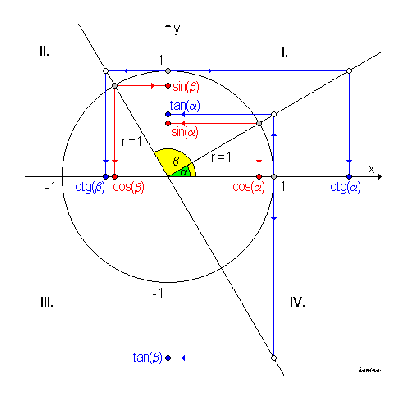
\epsfig{file=circle.eps,scale=1.5}
        \caption{Die Winkel-Funktionen am Einheitskreis.}
        \label{fig:circle}
      \end{figure}
      Aus der Definition von Sinus und Tangens folgt die Ungleichung 
      \\[0.3cm]
      \hspace*{1.3cm}
      $\sin(\varphi) \leq \varphi \leq \tan(\varphi) = \bruch{\sin(\varphi)}{\cos(\varphi)}$
      \\[0.3cm]
      Division dieser Gleichung durch $\sin(\varphi)$ liefert
      \\[0.3cm]
      \hspace*{1.3cm}
      $1 \leq \bruch{\varphi}{\sin(\varphi)} \leq \bruch{1}{\cos(\varphi)}$
      \\[0.3cm]
      Wir bilden den Kehrwert und erhalten
      \\[0.3cm]
      \hspace*{1.3cm}
      $1 \geq \bruch{\sin(\varphi)}{\varphi} \geq \cos(\varphi)$
      \\[0.3cm]
      Nun bilden wir den Grenzwert f�r $\varphi \rightarrow 0$:
      \\[0.3cm]
      \hspace*{1.3cm}
      $1 \geq \lim\limits_{\varphi \rightarrow 0} \bruch{\sin(\varphi)}{\varphi} \geq \lim\limits_{\varphi \rightarrow 0}\cos(\varphi)$
      \\[0.3cm]
      Wegen $\lim_{\varphi \rightarrow 0} \cos(\varphi) = \cos(0) = 1$ folgt daraus
      \\[0.3cm]
      \hspace*{1.3cm}
      $\lim\limits_{\varphi \rightarrow 0} \bruch{\sin(\varphi)}{\varphi} = 1$.
      \\[0.3cm]
       Aus dem Geometrie-Untericht ist das Additionstheorem f�r den Sinus 
       bekannt: 
       \\[0.3cm]
       \hspace*{1.3cm} $\sin(x+y) = \sin(x) \cdot \cos(y) + \cos(x) \cdot \sin(y)$.
         \\[0.2cm]
       Daraus folgt einerseits
       \\[0.3cm]
       \hspace*{1.3cm}
       $
       \begin{array}[t]{lcl}
         \sin(x) & = & \sin\left(\frac{x + y}{2} + \frac{x - y}{2}\right) \\[0.3cm]
                 & = & \sin\left(\frac{x + y}{2}\right)\cdot \cos\left(\frac{x - y}{2}\right) + \cos\left(\frac{x + y}{2}\right)\cdot \sin\left(\frac{x - y}{2}\right) 
       \end{array}
       $
       \\[0.3cm]
       und andererseits gilt wegen $\sin(-x) = -\sin(x)$ und $\cos(-x) = \cos(x)$
       \\[0.3cm]
       \hspace*{1.3cm}
       $
       \begin{array}[t]{lcl}
         \sin(y) & = & \sin\left(\frac{x + y}{2} - \frac{x - y}{2}\right) \\[0.3cm]
                 & = & \sin\left(\frac{x + y}{2}\right)\cdot \cos\left(\frac{x - y}{2}\right) - \cos\left(\frac{x + y}{2}\right)\cdot \sin\left(\frac{x - y}{2}\right). 
       \end{array}
       $
       \\[0.3cm]
       Subtrahieren wir diese Gleichungen voneienander, so erhalten wir 
       \\[0.3cm]
       \hspace*{1.3cm}
       $\sin(x) - \sin(y) = 2 \cdot \cos\left(\frac{x + y}{2}\right)\cdot \sin\left(\frac{x - y}{2}\right)$.
       \\[0.3cm]
       Damit k�nnen wir die Ableitung des Sinus ausrechnen:
       \\[0.3cm]
       \hspace*{1.3cm}
       $
       \begin{array}[t]{lcl}
       \lim\limits_{h \rightarrow 0} \bruch{\sin(x+h)-\sin(x)}{h} & = &
       \lim\limits_{h \rightarrow 0} \bruch{2 \cdot \cos\left(\frac{x + h + x}{2}\right)\cdot \sin\left(\frac{x + h - x}{2}\right)}{h} \\[0.3cm]
        & = &
        \lim\limits_{h \rightarrow 0} \cos\left(x + \frac{h}{2}\right) \cdot \lim\limits_{h \rightarrow 0} \bruch{\sin\left(\frac{h}{2}\right)}{\frac{h}{2}} \\[0.3cm]
        & = & \cos(x) \cdot \lim\limits_{h \rightarrow 0} \bruch{\sin\left(h\right)}{h} \\[0.3cm]
        & = & \cos(x) \\[0.3cm]
       \end{array}
       $
      \\[0.3cm]
      Damit haben wir gezeigt, dass gilt:
      \\[0.3cm]
      \hspace*{1.3cm}
      $\frac{d\;}{dx}\sin(x) = \cos(x)$.
\item Die Ableitung des Cosinus k�nnte in analoger Weise berechnet werden, es ist aber 
      einfacher, wenn wir von den Gleichungen
      \\[0.3cm]
      \hspace*{1.3cm}
      $\cos(x) = \sin\bigl(\frac{\pi}{2}- x\bigr)$ \quad und \quad $\cos(\frac{\pi}{2}- x\bigr) = \sin(x)$
      \\[0.3cm]
      ausgehen und die Ketten-Regel verwenden. Es ergibt sich
      \\[0.3cm]
      \hspace*{1.3cm}
      $
      \begin{array}[t]{lcll}
      \dfo\cos(x) & = & \dfo\sin\Bigl(\frac{\pi}{2}- x\Bigr) \\[0.3cm]
                 & = & \cos\Bigl(\frac{\pi}{2}- x\Bigr) \cdot \dfo\Bigl(\frac{\pi}{2}- x\Bigr) & \mbox{nach der Ketten-Regel} \\[0.3cm]
                 & = & \sin(x) \cdot (-1) \\[0.3cm]
                 & = & -\,\sin(x). \\[0.3cm]
      \end{array}$
\item Jetzt kann die Ableitung der Tangens-Funktion �ber die Quotienten-Regel berechnet 
      werden: 
      \\[0.3cm]
      \hspace*{1.3cm}
      $\displaystyle
      \begin{array}[t]{lcl}
      \ds \frac{d\;}{dx} \tan(x) & = & \ds\frac{d\;}{dx} \left(\bruch{\sin(x)}{\cos(x)}\right) \\[0.3cm]
      & = & \bruch{\Bigl(\frac{d\;}{dx} \sin(x)\Bigr) \cdot \cos(x) - \sin(x) \cdot \Bigl(\frac{d\;}{dx} \cos(x)\Bigr)}{\cos^2(x)} \\[0.5cm]
      & = & \bruch{\cos(x) \cdot \cos(x) - \sin(x) \cdot \bigr(-\sin(x)\bigr)}{\cos^2(x)} \\[0.5cm]
      & = & \bruch{\cos^2(x) + \sin^2(x)}{\cos^2(x)} \\[0.5cm]
      & = & \bruch{1}{\cos^2(x)} \\[0.5cm]
      \end{array}
      $
\item Die Ableitung der Arcus-Tangens-Funktion kann nun mit dem selben Trick berechnet werden,
      den wir schon bei der Berechnung der Ableitung des Logarithmus benutzt haben.
      Wir gehen diesmal von der Gleichungen 
      \\[0.2cm]
      \hspace*{1.3cm}
      $\arctan\bigl(\tan(x)\bigr) = x$
      \\[0.2cm]
      aus und differenzieren beide Seiten dieser Gleichung.  Nach der Ketten-Regel erhalten wir 
      \\[0.3cm]
      \hspace*{1.3cm}
      $\arctan'\bigl(\tan(x)\bigr) \cdot \frac{d\;}{dx} \tan(x) = 1$.
      \\[0.3cm]
      Setzen wir hier die Ableitung f�r die Tangens-Funktion ein, so haben wir
      \\[0.3cm]
      \hspace*{1.3cm}
      $\ds \frac{d\;}{dx} \arctan\bigl(\tan(x)\bigr) \cdot \bruch{1}{\cos^2(x)} = 1$.
      \\[0.3cm]
      Multiplikation mit $\cos^2(x)$ ergibt
      \\[0.3cm]
      \hspace*{1.3cm}
      $\ds \frac{d\;}{dx} \arctan\bigl(\tan(x)\bigr) = \cos^2(x)$.
      \\[0.3cm]
      Den in dieser  Gleichung auftretenden Term $\cos^2(x)$ m�ssen wir durch einen Term ausdr�cken, in dem
      nur $\tan(x)$ auftritt.  Dazu betrachten wir die Definition der Tangens-Funktion:      
      \\[0.3cm]
      \hspace*{1.3cm}
      $
      \begin{array}[t]{lrcll}
                & \tan^2(x) & = & \bruch{\sin^2(x)}{\cos^2(x)} \\[0.5cm] 
\Leftrightarrow & \tan^2(x) & = & \bruch{1 - \cos^2(x)}{\cos^2(x)} & \mbox{wegen}\; \sin^2(x) + \cos^2(x) = 1 \\[0.5cm] 
\Leftrightarrow & \cos^2(x) \cdot \tan^2(x) & = & 1 - \cos^2(x) &  \\[0.3cm] 
\Leftrightarrow & \cos^2(x) \cdot \tan^2(x) + \cos^2(x) & = & 1  &  \\[0.3cm] 
\Leftrightarrow & \cos^2(x) \cdot \bigr(\tan^2(x) + 1\bigr) & = & 1  &  \\[0.3cm] 
\Leftrightarrow & \cos^2(x)  & = &  \bruch{1}{\tan^2(x) + 1} &  
      \end{array}
      $
      \\[0.3cm]
      Damit k�nnen wir also schreiben 
      \\[0.3cm]
      \hspace*{1.3cm}
      $\arctan'\bigl(\tan(x)\bigr) = \bruch{1}{\tan^2(x) + 1}$.
      \\[0.3cm]
      Setzen wir jetzt $y = \tan(x)$, so erhalten wir 
      \\[0.3cm]
      \hspace*{1.3cm}
      $\displaystyle\frac{d\;}{dy} \arctan(y) = \bruch{1}{y^2 + 1}$.
\end{enumerate}

\exercise
Zeigen Sie 
\\[0.3cm]
\hspace*{1.3cm} $\ds\frac{d\;}{dx} \arcsin(x) = \bruch{1}{\sqrt{1 - x^2}}$.  \eox



\exercise
Berechnen Sie die Ableitung der Funktion $x \mapsto \sqrt{x}$.  
\vspace*{0.3cm}

\noindent
\textbf{Hinweis}: Verwenden Sie die Produkt-Regel. \eox

\exercise
Es sei $p \in \mathbb{Z}$ und $q \in \mathbb{N}$.  �berlegen Sie, was die Ableitung der Funktion
\\[0.2cm]
\hspace*{1.3cm}
$\ds x \mapsto x^{\frac{p}{q}}$
\\[0.2cm]
ist und beweisen Sie Ihre Behauptung.
\vspace*{0.3cm}

\noindent
\textbf{Hinweis}: Betrachten Sie zun�chst den Fall $p = 1$.  \eox


\section{Mittelwert-S�tze}
\begin{Definition}[lokales Maximum]
  Eine Funktion $f:\mathbb{R} \rightarrow \mathbb{R}$ hat im Punkt $\bar{x}\in \mathbb{R}$ ein \emph{lokales Maximum}, wenn gilt:
  \\[0.2cm]
  \hspace*{1.3cm}
  $\exists \varepsilon \in \mathbb{R}_+: \forall x \in \mathbb{R}: |x - \bar{x}| < \varepsilon
  \rightarrow f(x) \leq f(\bar{x})$.
  \eod
\end{Definition}

Die in der obigen Definition auftretende Menge von Zahlen, deren Abstand von $\bar{x}$
kleiner ist als $\varepsilon$, bezeichnen wir auch als $\varepsilon$-Umgebung des Punktes
$\bar{x}$, die $\varepsilon$-Umgebung des Punktes $x$ ist also die Menge 
\\[0.2cm]
\hspace*{1.3cm} $U_\varepsilon(\bar{x}) := \bigl\{ x \in \mathbb{R} \;\big|\; |x - \bar{x}| < \varepsilon \bigr\}$.
\\[0.2cm]
Der Begriff des lokalen Maximums steht im Kontrast zu dem Begriff eines \emph{globalen Maximums}.
Eine Funktion $f:D \rightarrow \mathbb{R}$ hat in einem Punkt $\bar{x} \in D$ ein globales
Maximum, wenn
\\[0.2cm]
\hspace*{1.3cm}
$\forall x \in D: f(x) \leq f(\bar{x})$
\\[0.2cm]
gilt.  Nat�rlich ist jedes globale Maximum auch ein lokales Maximum, aber die Umkehrung
gilt im allgemeinen nicht.  Der n�chste Satz liefert ein notwendiges Kriterium f�r das
Auftreten eines lokalen Maximums.

\begin{Satz}[\href{http://en.wikipedia.org/wiki/Fermat}{Pierre de Fermat}, 160?--1665]
Hat die Funktion $f: D \rightarrow \mathbb{R}$ im Punkt $\bar{x}$ ein lokales
Maximum, ist $U_\varepsilon(\bar{x}) \subseteq D$ und ist die Funktion $f$ zus�tzlich im Punkt $\bar{x}$ differenzierbar, so gilt 
\\[0.3cm]
\hspace*{1.3cm}
$\df{f}(\bar{x}) = 0$.
\end{Satz}

\proof
Wir betrachten zun�chst die Folge $\folge{\bar{x} + \frac{1}{n}}$.
O.B.d.A. sei $\varepsilon$ so klein gew�hlt, dass 
\\[0.2cm]
\hspace*{1.3cm}
$\forall x \in \mathbb{R} : |x - \bar{x}| < \varepsilon \rightarrow f(x) \leq f(\bar{x})$
\\[0.2cm]
gilt.  Wenn $n>\frac{1}{\varepsilon}$ ist, liegt  $\bar{x} + \frac{1}{n}$ in der
$\varepsilon$-Umgebung von $\bar{x}$.  Daher gilt f�r alle $n > \frac{1}{\varepsilon}$
\\[0.3cm]
\hspace*{1.3cm}
 $f\bigl(\bar{x} + \frac{1}{n}\bigr) \leq f(\bar{x})$. 
\\[0.3cm]
Damit gilt f�r den Differential-Quotienten
\\[0.3cm]
\hspace*{1.3cm}
$\bruch{f\Bigl(\bar{x} + \frac{1}{n}\Bigr) - f(\bar{x})}{\bar{x} + \frac{1}{n} - \bar{x}} \;=\;
 n \cdot \left(f\Bigl(\bar{x} + \frac{1}{n}\Bigr) - f(\bar{x})\right) \leq 0$. 
\\[0.3cm]
Da wir vorausgesetzt haben, dass die Funktion $f$ im Punkt $\bar{x}$ differenzierbar ist,
gilt 
\\[0.3cm]
\hspace*{1.3cm}
$\df{f}(\bar{x}) = \lim\limits_{n \rightarrow \infty} \bruch{f\Bigl(\bar{x} + \frac{1}{n}\Bigr) - f(\bar{x})}{\bar{x} + \frac{1}{n} - \bar{x}} \leq 0$.
\\[0.3cm]
Wir betrachten nun die Folge $\folge{\bar{x} - \frac{1}{n}}$.
Wieder sei $\varepsilon$ so gew�hlt, dass 
\\[0.2cm]
\hspace*{1.3cm}
$\forall x \in \mathbb{R} : |x - \bar{x}| < \varepsilon \rightarrow f(x) \leq f(\bar{x})$
\\[0.2cm]
gilt.  Wenn $n>\frac{1}{\varepsilon}$ liegt daher  $\bar{x} - \frac{1}{n}$ in der
$\varepsilon$-Umgebung von $\bar{x}$.  Daher gilt f�r alle $n > \frac{1}{\varepsilon}$
\\[0.3cm]
\hspace*{1.3cm} $f\bigl(\bar{x} - \frac{1}{n}\bigr) \leq f(\bar{x})$. 
\\[0.3cm]
Damit gilt f�r den Differential-Quotienten
\\[0.3cm]
\hspace*{1.3cm}
$\bruch{f\Bigl(\bar{x} + \frac{1}{n}\Bigr) - f(\bar{x})}{\bar{x} - \frac{1}{n} - \bar{x}} \;=\;
 - n \cdot \left(f\Bigl(\bar{x} - \frac{1}{n}\Bigr) - f(\bar{x})\right) \geq 0$. 
\\[0.3cm]
Da wir vorausgesetzt haben, dass die Funktion $f$ im Punkt $\bar{x}$ differenzierbar ist,
gilt 
\\[0.3cm]
\hspace*{1.3cm}
$\df{f}(\bar{x}) = \lim\limits_{n \rightarrow \infty} \bruch{f\Bigl(\bar{x} - \frac{1}{n}\Bigr) - f(\bar{x})}{\bar{x} - \frac{1}{n} - \bar{x}} \geq 0$.
\\[0.3cm]
Wir haben jetzt also die beiden Ungleichungen 
\\[0.3cm]
\hspace*{1.3cm}
$\df{f}(\bar{x}) \leq 0$ \quad und \quad $\df{f}(\bar{x}) \geq 0$ 
\\[0.3cm]
gezeigt.  Daraus folgt sofort $\df{f}(\bar{x}) = 0$. \hspace*{\fill} $\Box$
\vspace*{0.3cm}

\noindent
Analog zur Definition eines lokalen Maximums kann auch der Begriff eines \emph{lokalen Minimums}
definiert werden.  Auch in einem lokalen Minimum hat die Ableitung den Wert 0.

\begin{Satz}
 Ist die Funktion $f:[a,b] \rightarrow \mathbb{R}$ stetig, so nimmt $f$ auf dem Intervall
 $[a,b]$ sowohl das Maximum als auch das Minimum an, es gibt also Punkte
 $x_{\textsl{\footnotesize min}}$ und  $x_{\textsl{\footnotesize max}}$, so dass gilt 
 \\[0.2cm]
 \hspace*{1.3cm}
 $\forall x \in [a,b]: f(x) \leq f(x_{\textsl{\footnotesize max}})$ \quad und \quad $\forall x \in [a,b]: f(x) \geq f(x_{\textsl{\footnotesize min}})$.
\eox
\end{Satz}


\begin{Satz}[\href{http://en.wikipedia.org/wiki/Michel_Rolle}{Michel Rolle}, 1652 -- 1719]
  Ist die Funktion \mbox{$f:[a,b]\rightarrow \mathbb{R}$} differenzierbar und gilt au�er\-dem $f(a) = f(b)$, dann gibt es ein
  $\bar{x} \in (a,b)$, so dass gilt 
  \\[0.3cm]
  \hspace*{1.3cm}
  $\df{f}(\bar{x}) = 0$.  
\end{Satz}

\noindent
\textbf{Beweis}: Es gibt zwei
F�lle:
\begin{enumerate}
\item Die Funktion $f$ ist konstant, f�r alle $x\in[a,b]$ gilt also $f(x) = f(a)$.
      Da die Ableitung einer konstanten Funktion den Wert $0$ hat, gilt dann offenbar sogar f�r alle $x\in[a,b]$ 
      \\[0.3cm]
      \hspace*{1.3cm} $\df{f}(x) = 0$.
\item Da die Funktion $f$ differenzierbar ist, ist sie auch stetig und nimmt
      daher sowohl ein Minimum als auch ein Maximum in dem Intervall $[a,b]$ an.  
      Es gibt also  $x_{\textsl{\footnotesize min}}$ und  $x_{\textsl{\footnotesize max}}$
      mit
      \\[0.2cm]
      \hspace*{1.3cm}
      $\forall x \in [a,b]: f(x) \leq f(x_{\textsl{\footnotesize max}})$ \quad und \quad $\forall x \in [a,b]: f(x) \geq f(x_{\textsl{\footnotesize min}})$.
      \\[0.2cm]
      Da wir jetzt voraussetzen k�nnen, dass die Funktion nicht konstant ist, und da
      weiterhin $f(a) = f(b)$ gilt, muss 
      \\[0.2cm]
      \hspace*{1.3cm}
      $f\bigl(x_{\textsl{\footnotesize min}}\bigr) < f(a)$ \quad  oder \quad
      $f\bigl(x_{\textsl{\footnotesize max}}\bigr) > f(a)$
      \\[0.2cm]
      gelten.  Daraus folgt 
      \\[0.2cm]
      \hspace*{1.3cm}
      $x_{\textsl{\footnotesize min}}\not\in \{a,b\}$ \quad  oder \quad $x_{\textsl{\footnotesize max}}\not\in \{a,b\}$.
      \\[0.2cm]
      Damit hat die Funktion dann in $x_{\textsl{\footnotesize min}}$ ein
      lokales Minimum oder in $x_{\textsl{\footnotesize max}}$ ein lokales
      Maximum (oder beides) und nach dem Satz von Fermat folgt 
      \\[0.3cm]
      \hspace*{1.3cm}
      $\df{f}\bigl(x_{\textsl{\footnotesize min}}\bigr) = 0$ \quad  oder \quad $\df{f}\bigl(x_{\textsl{\footnotesize max}}\bigr) = 0$.
      \hspace*{\fill} $\Box$
\end{enumerate}
Aus dem Satz von Rolle folgern wir sp�ter zwei wichtige Mittelwert-S�tze und den Satz von 
\textsl{L'H\^opital} (Guillaume Fran\c{c}ois Antoine, Marquis de L'H\^opital, 1661--1704).

\begin{Satz}[Mittelwert-Satz der Differential-Rechnung, \href{http://de.wikipedia.org/wiki/Augustin-Louis_Cauchy}{Augustin-Louis Cauchy}, 1789--1857]
  Ist die Funktion $f:[a,b] \rightarrow \mathbb{R}$ f�r alle $x\in[a,b]$ differenzierbar, 
  so gilt: 
  \\[0.3cm]
  \hspace*{1.3cm}
  $\exists c \in (a,b): \df{f}(c) = \bruch{f(b) - f(a)}{b - a}$.
\end{Satz}

\noindent
\textbf{Beweis}: Wir definieren die Funktion $g:[a,b] \rightarrow \mathbb{R}$ durch
\\[0.3cm]
\hspace*{1.3cm} $g(x) := f(x) - f(a) - \bruch{f(b) - f(a)}{b-a}\cdot (x-a)$.
\\[0.3cm]
Da die Funktion $f$ nach Voraussetzung differenzierbar ist, ist auch die Funktion $g$ differenzierbar und es gilt 
\\[0.3cm]
\hspace*{1.3cm}
$g(a) = f(a) - f(a) - \bruch{f(b) - f(a)}{b-a}\cdot (a-a) =0$.
\\[0.0cm]
und
\\[0.0cm]
\hspace*{1.3cm} $g(b) = f(b) - f(a) - \bruch{f(b) - f(a)}{b-a}\cdot (b-a) = f(b) - f(a) - \bigl(f(b) - f(a)\bigr) = 0$.
\\[0.3cm]
Damit gilt $g(a) = g(b)$ und folglich erf�llt die Funktion $g$ die Voraussetzung des Satzes von Rolle.  Also gibt es ein
$c \in (a,b)$, so dass 
\\[0.3cm]
\hspace*{1.3cm}
$\df{g}(c) = 0$
\\[0.3cm]
gilt.  Setzen wir hier die Definition von $g$ ein, so haben wir 
\\[0.3cm]
\hspace*{1.3cm}
$
\begin{array}[b]{ll}
            & \df{g}(c) = \df{f}(c) - \bruch{f(b) - f(a)}{b-a} = 0 \\[0.3cm]
\Rightarrow & \df{f}(c) = \bruch{f(b) - f(a)}{b-a}
\end{array}
$
\hspace*{\fill} $\Box$
\vspace*{0.3cm}

Abbildung \ref{fig:mean-value-theorem} zeigt die geometrische Bedeutung des
Mittelwert-Satzes:  Es gibt eine Tangente an die Funktion, die die selbe Steigung hat wie
die Sekante, die durch die Punkte $\pair(a,f(a))$ und $\pair(b,f(b))$  geht.
      \begin{figure}[!h]
        \centering
        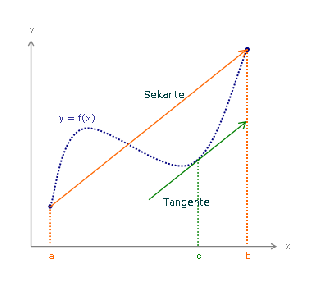
\epsfig{file=mean-value-theorem.eps,scale=1.5}
        \caption{Geometrische Bedeutung des Mittelwert-Satzes.}
        \label{fig:mean-value-theorem}
      \end{figure}

\pagebreak

\begin{Satz}[Erweiterter Mittelwert-Satz]
  Sind die Funktion $f,g:[a,b] \rightarrow \mathbb{R}$ f�r alle $x\in[a,b]$
  differenzierbar und gilt $\df{g}(x) \not= 0$ f�r alle $x \in [a,b]$,
  so gilt: 
  \\[0.3cm]
  \hspace*{1.3cm}
  $\exists c \in (a,b): \bruch{f'(c)}{g'(c)} = \bruch{f(b) - f(a)}{g(b) - g(a)}$.
  \eox
\end{Satz}

\noindent
\textbf{Bemerkung}: Auf den ersten Blick mag es verwundern, dass nicht explizit 
$g(a) \not = g(b)$ gefordert wird.  Dies folgt aber sofort aus der Bedingung
$\forall x \in [a,b]:\df{g}(x) \not= 0$ und dem Satz von Rolle. \eox
\vspace*{0.3cm}

\exercise
Beweisen Sie den erweiterten Mittelwert-Satz.  Betrachten Sie dazu die Funktion
\\[0.2cm]
\hspace*{1.3cm}
$h(x) := \alpha \cdot f(x) - \beta \cdot g(x)$
\\[0.2cm]
und bestimmen Sie $\alpha$ und $\beta$ so, dass Sie auf die Funktion $h$ den Satz von Rolle anwenden k�nnen. \eox

% \solution
% Nach dem Mittelwert-Satz der Differential-Rechnung gibt es ein $c \in [a,b]$, so dass
% \\[0.2cm]
% \hspace*{1.3cm}
% $\ds \df{h}(c) = \frac{h(b) - h(a)}{b - a}$
% \\[0.2cm]
% gilt.  Wir berechnen die Werte von $h$, die in dieser Gleichung eine Rolle spielen, getrennt.
% \begin{enumerate}
% \item $h(a) = \bigl(g(b) - g(a) \bigr) \cdot f(a) - \bigl(f(b) - f(a)\bigr) \cdot g(a)$, 
% \item $h(b) = \bigl(g(b) - g(a) \bigr) \cdot f(b) - \bigl(f(b) - f(a)\bigr) \cdot g(b)$,
% \item $\df{h}(x) = \bigl(g(b) - g(a) \bigr) \cdot \df{f}(x) - \bigl(f(b) - f(a)\bigr) \cdot \df{g}(x)$.
% \end{enumerate}
% Damit finden wir
% \\[0.2cm]
% \hspace*{0.3cm}
% $
% \begin{array}[t]{lcrl}
% h(b) - h(a) & = &   & \bigl(g(b) - g(a) \bigr) \cdot f(b) - \bigl(f(b) - f(a)\bigr) \cdot g(b) \\[0.1cm]
%             &   & - & \bigl(g(b) - g(a) \bigr) \cdot f(a) + \bigl(f(b) - f(a)\bigr) \cdot g(a) \\[0.2cm]
%             & = &   & \bigl(g(b) - g(a) \bigr) \cdot \bigl(f(b) - f(a)\bigr) - \bigl(f(b) - f(a)\bigr) \cdot \bigl(g(b) - g(a) \bigr) \\[0.2cm]
%             & = &   & 0.
% \end{array}
% $
% \\[0.2cm]
% Nach dem Satz von Rolle finden wir also ein $c \in [a,b]$, so dass $\df{h}(c) = 0$ ist.  Setzen wir
% $c$ in die Formel f�r $\df{h}(x)$ ein, so erhalten wir
% \\[0.2cm]
% \hspace*{1.3cm}
% $0 = \bigl(g(b) - g(a) \bigr) \cdot \df{f}(c) - \bigl(f(b) - f(a)\bigr) \cdot \df{g}(c)$
% \\[0.2cm]
% Daraus folgt
% \\[0.2cm]
% \hspace*{1.3cm}
% $\ds \frac{f'(c)}{g'(c)} = \frac{f(b) - f(a)}{g(b) - g( a)}$ 
% \\[0.2cm]
% und das ist die Behauptung.
% \qed

Der folgende Satz ist f�r die praktische Berechnung von Grenzwerten unentbehrlich.

\begin{Satz}[Guillaume Fran\c{c}ois Antoine, Marquis de L'H\^opital, 1661 --1704] \lb 
  Die Funktionen $f,g: (a,b) \rightarrow \mathbb{R}$ seien
  differenzierbar , es sei $c \in (a,b)$ und es gelte
  \begin{enumerate}
  \item $f(c) = g(c) = 0$
  \item $\forall x \in (a,b):  g'(x) \not= 0$.
  \item $\lim\limits_{x \rightarrow a} \bruch{f'(x)}{g'(x)}$ existiert.
  \end{enumerate}
  Dann gilt 
  \\[0.3cm]
  \hspace*{1.3cm}
  $\lim\limits_{x \rightarrow c} \bruch{f(x)}{g(x)} = 
   \lim\limits_{x \rightarrow c} \bruch{f'(x)}{g'(x)}$.
\end{Satz}

\noindent
\textbf{Beweis}: 
Da die Funktion $f$ und $g$ im Punkt $c$ differenzierbar sind, gibt es Funktionen $r_1(h)$
und $r_2(h)$, so dass gilt:
\begin{enumerate}
\item $f(c+h) = f(c) + h\cdot f'(c) + r_1(h)$ \quad mit $\lim\limits_{h \rightarrow 0} \bruch{r_1(h)}{h} = 0$.
\item $g(c+h) = g(c) + h\cdot g'(c) + r_2(h)$ \quad mit $\lim\limits_{h \rightarrow 0} \bruch{r_2(h)}{h} = 0$.
\end{enumerate}
Wir haben die folgende Kette von Gleichungen:
\\[0.3cm]
\hspace*{1.3cm}
$
\begin{array}[b]{lclcl}
    \lim\limits_{h \rightarrow 0} \bruch{f(c+h)}{g(c+h)} &=&
    \lim\limits_{h \rightarrow 0} \bruch{f(c) + h\cdot f'(c) + r_1(h)}{g(c) + h\cdot g'(c) + r_2(h)} 
&=& \lim\limits_{h \rightarrow 0} \bruch{h\cdot f'(c) + r_1(h)}{h\cdot g'(c) + r_2(h)} \\[0.5cm]
&=& \lim\limits_{h \rightarrow 0} \bruch{f'(c) + \frac{r_1(h)}{h}}{g'(c) + \frac{r_2(h)}{h}} 
&=& \bruch{f'(c) + \lim\limits_{h \rightarrow 0} \frac{r_1(h)}{h}}{g'(c) + \lim\limits_{h \rightarrow 0} \frac{r_2(h)}{h}} \\[0.8cm]
&=& \bruch{f'(c)}{g'(c)} \\[0.5cm]
\end{array}
$
\hspace*{\fill} $\Box$
\vspace*{0.3cm}
\pagebreak

\example
Mit dem Satz von L'H\^opital k�nnen wir nun den Grenzwert
$\ds\lim\limits_{x \rightarrow 0} \frac{\sin(x)}{x}$ noch einmal berechnen: 
\\[0.3cm]
\hspace*{1.3cm} $\ds\lim\limits_{x \rightarrow 0} \frac{\sin(x)}{x} = \lim\limits_{x \rightarrow 0}
\frac{\cos(x)}{1} = \cos(0) = 1$.
\eox
\vspace*{0.3cm}

\noindent
Der Satz von L'H\^opital beh�lt seine G�ltigkeit, wenn $x$ gegen Unendlich strebt.  Sind 
$f,g:\mathbb{R} \rightarrow \mathbb{R}$ differenzierbare Funktionen, so dass der Grenzwert
\\[0.3cm]
\hspace*{1.3cm}
$\lim\limits_{x \rightarrow \infty} \frac{f'(x)}{g'(x)}$ 
\\[0.3cm]
existiert, und gilt entweder 
\\[0.3cm]
\hspace*{0.3cm}
$\Bigl(\lim\limits_{x \rightarrow \infty} f(x) = 0 \;\wedge\; \lim\limits_{x \rightarrow \infty} g(x) = 0\Bigr) \quad \vee \quad
 \Bigl(\lim\limits_{x \rightarrow \infty} f(x) = \infty \;\wedge\;\lim\limits_{x \rightarrow \infty} g(x) = \infty\Bigr)$ 
\\[0.3cm]
so folgt
\\
\hspace*{1.3cm}
$\ds\lim\limits_{x \rightarrow \infty} \frac{f(x)}{g(x)} = \lim\limits_{x \rightarrow \infty} \frac{f'(x)}{g'(x)}$.
\\[0.3cm]
Wir geben ein Beispiel.  Es gilt 
\\[0.3cm]
\hspace*{1.3cm}
$\ds\lim\limits_{x \rightarrow \infty} \frac{x}{\exp(x)} = \lim\limits_{x \rightarrow \infty} \frac{1}{\exp(x)} = 0$.
\\[0.3cm]
Der Satz von L'H\^opital l��t sich iteriert anwenden.  Beispielsweise gilt
\\[0.3cm]
\hspace*{1.3cm}
$\ds\lim\limits_{x \rightarrow \infty} \frac{x^2}{\exp(x)} = \lim\limits_{x \rightarrow \infty} \frac{2\cdot x}{\exp(x)} =\lim\limits_{x \rightarrow \infty} \frac{2}{\exp(x)} = 0$.
\vspace*{0.3cm}

\begin{Definition}[Schnelleres Wachstum]
  Wir sagen, dass die Funktion $x \mapsto f(x)$ f�r $x \rightarrow \infty$ \emph{schneller als} die
  Funktion $x \mapsto g(x)$ \emph{w�chst}, falls 
  \\[0.2cm]
  \hspace*{1.3cm}
  $\ds \lim\limits_{x \rightarrow \infty} \frac{g(x)}{f(x)} = 0$
  \\[0.2cm]
  gilt. \eox
\end{Definition}

\exercise
Zeigen Sie, dass f�r alle nat�rlichen Zahlen $n$ gilt: 
\\[0.3cm]
\hspace*{1.3cm} $\lim\limits_{x \rightarrow \infty} \bruch{x^n}{\exp(x)} = 0$.
\\[0.3cm]
Damit sehen wir, dass die Exponential-Funktion schneller w�chst als jede Potenz.  
\eox

\exercise
\begin{enumerate}
\item Zeigen Sie, dass die Funktion $\ds x \mapsto e^{\ln(x) \cdot \ln(x)}$ f�r alle $n \in \mathbb{N}$ schneller
      als die Funktion $x \mapsto x^n$ w�chst.
\item Zeigen Sie, dass die Funktion $\ds x \mapsto e^x$ schneller w�chst als die Funktion
      $\ds x \mapsto e^{\ln(x) \cdot \ln(x)}$. \eox
\end{enumerate} 

\exercise
Berechnen Sie den Grenzwert
\\[0.2cm]
\hspace*{1.3cm}
$\ds\lim\limits_{x \rightarrow 0} x \cdot \ln(x)$.  \eox
\pagebreak

\exercise
Berechnen Sie den Grenzwert
\\[0.2cm]
\hspace*{1.3cm}
$\ds\lim\limits_{x \rightarrow \infty} \sqrt{x + \sqrt{x\;}\;} - \sqrt{x\;}$.  \eox


\section{Monotonie und Konvexit�t}
\begin{Definition}[monoton]
  Eine Funktion $f: D \rightarrow \mathbb{R}$ ist \emph{monoton steigend} g.d.w.
  \\[0.2cm]
  \hspace*{1.3cm}
  $\forall x,y \in D: x < y \rightarrow f(x) \leq f(y)$
  \\[0.2cm]
  gilt.  Die Funktion $f$ ist \emph{streng monoton steigend}, wenn die sch�rfere Bedingung
  \\[0.2cm]
  \hspace*{1.3cm}
  $\forall x,y \in D: x < y \rightarrow f(x) < f(y)$
  \\[0.2cm]
  erf�llt ist.  Weiter hei�t  $f$ \emph{monoton fallend}, wenn
  \\[0.2cm]
  \hspace*{1.3cm}
  $\forall x,y \in D: x < y \rightarrow f(x) \geq f(y)$
  \\[0.2cm]
  gilt.  Analog ist $f$ \emph{streng monoton fallend}, falls die folgende Bedingung gilt:
  \\[0.2cm]
  \hspace*{1.3cm}
  $\forall x,y \in D: x < y \rightarrow f(x) > f(y)$.
  \eod
\end{Definition}

\begin{Satz}
  Eine differenzierbare Funktion $f:D \rightarrow \mathbb{R}$ ist genau dann
  monoton steigend, wenn gilt: 
  \\[0.2cm]
  \hspace*{1.3cm} $\forall x \in D: f'(x) \geq 0$.
  \eod
\end{Satz}

\noindent
\textbf{Beweis}:  Wir nehmen zun�chst an, dass $f$ monoton steigend ist und zeigen, dass
dann $f'(x) \geq 0$ gilt.  Die Ableitung ist definiert als der Grenzwert 
\\[0.3cm]
\hspace*{1.3cm} $f'(x) = \lim\limits_{h \rightarrow 0} \bruch{f(x+h) - f(x)}{h}$.
\\[0.3cm]
Wir zeigen, dass der Differential-Quotient 
\\[0.3cm]
\hspace*{1.3cm} $\bruch{f(x+h) - f(x)}{h}$
\\[0.3cm]
f�r alle $h \not = 0$ gr��er oder gleich 0 ist.  Zm Nachweis dieser Behauptung f�hren wir
eine Fallunterscheidung bez�glich des Vorzeichens von $h$ durch.
\begin{enumerate}
\item Fall: $h > 0$.

      Dann folgt aus der Monotonie von $f$,  dass 
      $f(x+h) \geq f(x)$ ist.  Also gilt $f(x+h)-f(x) \geq 0$ und daraus folgt
      \\[0.3cm]
      \hspace*{1.3cm} $\bruch{f(x+h) - f(x)}{h} \geq 0$.
\item Fall: $h < 0$.

      Jetzt folgt aus der Monotonie von $f$ die Ungleichung 
      $f(x+h) \leq f(x)$.  Also haben wir  $f(x+h)-f(x) \leq 0$.  Wegen $h<0$ gilt dann
      \\[0.3cm]
      \hspace*{1.3cm} $\bruch{f(x+h) - f(x)}{h} \geq 0$.
\end{enumerate}
Da der Differential-Quotient in jedem Fall gr��er-gleich $0$ ist, muss $f'(x) \geq 0$
gelten.
\vspace*{0.2cm}

Wir nehmen nun an, dass f�r alle $x\in D$ die Ungleichung $f'(x) \geq 0$ gilt und
zeigen, dass $f$ dann monoton steigend ist.  Diesen Beweis f�hren wir indirekt.
Wir nehmen an, es g�be $x,y\in D$ mit 
\\[0.2cm]
\hspace*{1.3cm} $x < y$ \quad aber \quad $f(x) > f(y)$.
\\[0.2cm]
Nach dem Mittelwert-Satz der Differential-Rechnung gibt es dann ein $z\in[x,y]$, so dass
\\[0.3cm]
\hspace*{1.3cm} $f'(z) = \bruch{f(y) - f(x)}{y - x}$
\\[0.3cm]
gilt.  Aus $x < y$ folgt  $y - x \geq 0$ und aus $f(x) > f(y)$ folgt $f(y) - f(x) <0$.
Damit h�tten wir dann aber $f'(z) < 0$ im Widerspruch zur Voraussetzung.
\hspace*{\fill} $\Box$
\vspace*{0.3cm}

\noindent
In Analogie zum letzten Satz kann gezeigt werden, dass eine differenzierbare Funktion 
$f:D \rightarrow \mathbb{R}$ genau dann monoton
fallend ist, wenn f�r alle $x\in D$ die Ungleichung $f'(x) \leq 0$ gilt.

\exercise
Die Funktion $f:D \rightarrow \mathbb{R}$ sei differenzierbar und es gelte
\\[0.2cm]
\hspace*{1.3cm}
$\forall x \in D: f'(x) > 0$.
\\[0.2cm]
Zeigen Sie, dass die Funktion $f$ dann \underline{stren}g monoton steigend ist.
\vspace*{0.3cm}

\noindent
\textbf{Bemerkung:}
Die Funktion $x \mapsto x^3$ ist streng monoton steigend, aber an der Stelle $x=0$
verschwindet die Ableitung dieser Funktion.  Dies zeigt, dass sich die Aussage des letzten
Satzes nicht umkehren l��t.

\begin{Definition}[strenges lokales Minimum] \lb
  Eine Funktion $f:\mathbb{R} \rightarrow \mathbb{R}$ hat im Punkt $\bar{x}\in \mathbb{R}$
  ein \emph{strenges lokales Minimum}, wenn gilt:
  \\[0.2cm]
  \hspace*{1.3cm}
  $\exists \varepsilon \in \mathbb{R}_+: \forall x \in \mathbb{R}: 
  |x - \bar{x}| < \varepsilon \wedge\ x \not= \bar{x} \rightarrow f(x) > f(\bar{x})$.
\eod
\end{Definition}

\noindent
\textbf{Bemerkung}:  Der Begriff des \emph{strengen lokalen Maximum} l��t sich analog definieren.

\begin{Satz} \label{satz:minimum}
  Die Funktion $f:\mathbb{R} \rightarrow \mathbb{R}$ sei zweimal differenzierbar, die
  zweite Ableitung $f''(x)$ sei stetig und f�r
  ein $x_0 \in \mathbb{R}$ gelte
  \\[0.2cm]
  \hspace*{1.3cm}
  $f'(x_0) = 0 \;\wedge\; f''(x_0) > 0$.
  \\[0.2cm]
  Dann hat die Funktion $f$ in $x_0$ ein strenges lokales Minimum.
\end{Satz}

\proof Da die zweite Ableitung $f''(x)$ stetig ist, k�nnen wir $\varepsilon := f''(x_0) > 0$
setzen und finden dann ein $\delta > 0$, so dass
\\[0.2cm]
\hspace*{1.3cm} $\forall x \in \mathbb{R}: |x - x_0| < \delta \rightarrow |f''(x) - f''(x_0)|
< \varepsilon = f''(x_0)$.
\\[0.2cm]
gilt.  Daraus folgt, dass f�r alle $x \in \mathbb{R}$ mit $|x - x_0| < \delta$ die
Ungleichung
\\[0.2cm]
\hspace*{1.3cm} $f''(x_0) - |f''(x) - f''(x_0)| > 0$
\\[0.2cm]
gilt.  Wir behaupten, dass dann
\begin{equation}
  \label{eq:minimum}
 f''(x) > 0 \quad \mbox{f�r alle $x \in \mathbb{R}$ mit $|x - x_0| < \delta$} 
\end{equation}
gilt.
Zum Nachweis dieser Behauptung f�hren wir eine Fallunterscheidung bez�glich der relativen
Gr��e von $f''(x)$ und $f''(x_0)$ durch.
\begin{enumerate}
\item Fall: $f''(x) < f''(x_0)$.  Dann gilt 
      \\[0.2cm]
      \hspace*{1.3cm}
      $|f''(x) - f''(x_0)| = f''(x_0) - f''(x)$.
      \\[0.2cm]
      Also folgt aus der Ungleichung $f''(x_0) - |f''(x) - f''(x_0)| > 0$ die Ungleichung
      \\[0.2cm]
      \hspace*{1.3cm}
      $f''(x_0) - \bigl(f''(x_0) - f''(x)\bigr) > 0$
      \\[0.2cm]
      und wegen $f''(x_0) - \bigl(f''(x_0) - f''(x)\bigr) = f''(x)$ haben wir damit die Behauptung
      $f''(x) > 0$ gezeigt.
\item Fall: $f''(x) \geq f''(x_0)$.  

      In diesem Fall folgt die Behauptung sofort aus der Voraussetzung
      $f''(x_0) > 0$ und der Transitivit�t der Relation $>$.
\end{enumerate}
Die Ungleichung (\ref{eq:minimum}) zeigt uns, dass die Funktion $x \mapsto f'(x)$ in der $\delta$-Umgebung
von $x_0$ streng monoton steigend ist.  Da au�erdem $f'(x_0) = 0$ gilt, folgt insgesamt
\\[0.2cm]
\hspace*{1.3cm}
$f'(x) < 0$ \quad f�r alle $x\in U_\delta(x_0)$ mit $x < x_0$ \quad und \quad \\[0.2cm]
\hspace*{1.3cm}
$f'(x) > 0$ \quad f�r alle $x\in U_\delta(x_0)$ mit $x > x_0$.
\\[0.2cm]
Damit ist die Funktion $f$ innerhalb der $\delta$-Umgebung $U_\delta(x_0)$ f�r $x < x_0$
streng monoton fallend und f�r $x > x_0$ streng monoton wachsend.  Dann muss $f$ aber ein Minimum in
$x_0$ haben. \qed


\noindent
\textbf{Bemerkung}: Falls f�r die Funktion $f$ die Bedingung
\\[0.2cm]
\hspace*{1.3cm}
$f'(x_0) = 0 \wedge f''(x_0) < 0$.
\\[0.2cm]
erf�llt ist, dann hat die Funktion an der Stelle $x_0$ ein strenges lokales Maximum. \eox

\begin{Definition}[konvex, konkav]
Eine Funktion $f:\mathbb{R} \rightarrow \mathbb{R}$ hei�t \emph{konvex} genau dann, wenn 
\\[0.2cm]
\hspace*{1.3cm}
$\forall x_1,x_2 \in \mathbb{R}:\forall t\in [0,1]: 
  f\bigl(t \cdot x_1 + (1-t)\cdot x_2\bigr) \leq t \cdot f(x_1) + (1 - t) \cdot f(x_2)
$
\\[0.2cm]
gilt.  Geometrisch bedeutet dies, dass die Funktionswerte der Funktion $f$  unterhalb
der Sekante durch die Punkte 
$\bigl\langle x_1, f(x_1) \bigl\rangle$ und $\bigl\langle x_2, f(x_2) \bigl\rangle$
liegen.
\vspace*{0.2cm}

Eine Funktion $f:\mathbb{R} \rightarrow \mathbb{R}$ hei�t \emph{konkav} genau dann, wenn 
\\[0.2cm]
\hspace*{1.3cm}
$\forall x_1,x_2 \in \mathbb{R}:\forall t\in [0,1]: 
  f\bigl(t \cdot x_1 + (1-t)\cdot x_2\bigr) \geq t \cdot f(x_1) + (1 - t) \cdot f(x_2)
$
\\[0.2cm]
gilt.  Hier liegen die Funktionswerte der Funktion $f$ also oberhalb 
der Sekante durch die Punkte 
$\bigl\langle x_1, f(x_1) \bigl\rangle$ und $\bigl\langle x_2, f(x_2) \bigl\rangle$.
\eod
\end{Definition}

\begin{Lemma}[Invarianz der Konvexit�t unter linearen Transformationen]
  \label{lemma:konvex_invarianz} \lb
  Die Funktion $f:\mathbb{R} \rightarrow \mathbb{R}$ sei konvex und es sei $\alpha \in \mathbb{R}$.
  Definieren wir die Funktion $g:\mathbb{R} \rightarrow \mathbb{R}$ als
  \\[0.2cm]
  \hspace*{1.3cm}
  $g(x) := f(x) + \alpha \cdot x$,
  \\[0.2cm]
  so ist auch die Funktion $g$ konvex.  Eine entsprechende Aussage gilt auch f�r konkave Funktionen.
\end{Lemma}

\exercise
Beweisen Sie das vorangehende Lemma.

\begin{Satz}
Die Funktion $f:\mathbb{R} \rightarrow \mathbb{R}$ sei zweimal differenzierbar und die Funktion 
$x \mapsto f''(x)$ sei stetig.  Dann gilt 
\\[0.2cm]
\hspace*{1.3cm}
$f$  konvex \quad $\Leftrightarrow$ \quad $\forall x \in \mathbb{R}: f''(x) \geq 0$.
\end{Satz}

\noindent
\textbf{Beweis}: Wir spalten den Beweis in zwei Teile auf.
\begin{enumerate}
\item[``$\Rightarrow$'':] Wir f�hren den Nachweis indirekt und nehmen an, dass es ein $x_0 \in \mathbb{R}$
  gibt, so dass $f''(x_0) < 0$ ist.  �hnlich wie bei Beweis von Satz \ref{satz:minimum} folgt daraus, dass
  es eine $\delta_1$-Umgebung $U_{\delta_1}(x_0)$ gibt, so dass
  \\[0.2cm]
  \hspace*{1.3cm} $f''(x) < 0$ \quad f�r alle $x \in U_{\delta_1}(x_0)$ 
  \\[0.2cm]
  gilt.  Wir definieren eine Funktion $g:\mathbb{R} \rightarrow \mathbb{R}$ durch
  \\[0.2cm]
  \hspace*{1.3cm}
  $g(x) := f(x) - x \cdot f'(x_0)$.
  \\[0.2cm]
  Dann gilt 
  \\[0.2cm]
  \hspace*{1.3cm}
  $g'(x) = f'(x) - f'(x_0)$ \quad und \quad $g''(x) = f''(x)$.
  \\[0.2cm]
  Daraus folgt durch Einsetzen
  \\[0.2cm]
  \hspace*{1.3cm}
  $g'(x_0) = 0$ \quad und \quad $g''(x_0) < 0$.
  \\[0.2cm]
  Damit hat die Funktion $g$ im Punkt $x_0$ ein lokales Maximum.  Also gibt es eine $\delta_2$-Umgebung von
  $x_0$, so dass
  \\[0.2cm]
  \hspace*{1.3cm}
  $g(x) < g(x_0)$ \quad f�r alle $x \in U_{\delta_2}(x_0)$
  \\[0.2cm]
  gilt.  O.B.d.A. k�nnen wir voraussetzen, dass $\delta_2 \leq \delta_1$ gilt.  
  Nach dem Lemma \ref{lemma:konvex_invarianz} wissen wir, dass die Funktion $g$ ebenfalls konvex ist.
  Definieren wir $x_1 := x_0 - \frac{\delta_2}{2}$, $x_2 := x_0 + \frac{\delta_2}{2}$ und $t := \frac{1}{2}$,
  so folgt also
  \begin{equation}
    \label{eq:konvex1}
  t \cdot g(x_1) + (1 - t) \cdot g(x_2) \geq g\bigl(t \cdot x_1 + (1-t) \cdot x_2\bigr)    
  \end{equation}
  Nun gilt 
  \\[0.2cm]
  \hspace*{1.3cm}
  $t \cdot x_1 + (1-t) \cdot x_2 = 
   \frac{1}{2} \cdot x_0 - \frac{1}{2} \cdot\frac{\delta_2}{2} + 
   \frac{1}{2} \cdot x_0 + \frac{1}{2} \cdot\frac{\delta_2}{2}
   = x_0
  $.
  \\[0.2cm]
  Damit folgt aus der Ungleichung (\ref{eq:konvex1}) die Ungleichung
  \begin{equation}
    \label{eq:konvex2}    
  \frac{1}{2} \cdot g(x_1) + \frac{1}{2} \cdot g(x_2) \geq g(x_0)
  \end{equation} 
  Andererseits folgt aus der Tatsache, dass sowohl $x_1$ als auch $x_2$ in der $\delta_1$-Umgebung von $x_0$
  liegen, dass
  \\[0.2cm]
  \hspace*{1.3cm}
  $g(x_1) < g(x_0)$ \quad und \quad  $g(x_2) < g(x_0)$
  \\[0.2cm]
  gilt. Multiplizieren wir diese beiden Gleichungen mit $\frac{1}{2}$ und addieren sie, so ergibt sich
  \\[0.2cm]
  \hspace*{1.3cm}
  $\frac{1}{2} \cdot g(x_1) + \frac{1}{2} \cdot g(x_2) < g(x_0)$ .
  \\[0.2cm]
  Diese Ungleichung steht aber im Widerspruch zur Ungleichung (\ref{eq:konvex2}).
\item[``$\Leftarrow$'':]  Es seien $x_1$, $x_2$ und $t \in [0,1]$ gegeben.  O.B.d.A. sei weiter
  $x_1 < x_2$. Wir definieren zun�chst
  \\[0.2cm]
  \hspace*{1.3cm}
  $x_0 := t \cdot x_1 + (1 - t) \cdot x_2$
  \\[0.2cm]
  Es l��t sich sofort nachrechnen, dass dann $x_1 < x_0 < x_2$ gilt.  Nach dem Mittelwert-Satz der
  Differential-Rechnung gibt es jeweils ein $c_1 \in [x_1,x_0]$ und ein $c_2 \in [x_0,x_2]$, so dass
  \\[0.2cm]
  \hspace*{1.3cm}
  $f'(c_1) = \bruch{f(x_0) - f(x_1)}{x_0 - x_1}$  \quad und \quad
  $f'(c_2) = \bruch{f(x_2) - f(x_0)}{x_2 - x_0}$  
  \\[0.2cm]
  gilt.  Da $f''(x) \geq 0$ ist, wissen wir au�erdem, dass die Funktion $f'(x)$ monoton steigend ist.
  Da offenbar $c_1 \leq c_2$ ist, folgt daraus die Ungleichung $f'(c_1) \leq f'(c_2)$ und damit gilt
  \begin{equation}
    \label{eq:konvex3}
    \bruch{f(x_0) - f(x_1)}{x_0 - x_1} \leq \bruch{f(x_2) - f(x_0)}{x_2 - x_0}.    
  \end{equation}
  Es gilt
  \\[0.2cm]
  \hspace*{1.3cm}
  $x_0 - x_1 = t \cdot x_1 + (1 - t) \cdot x_2 - x_1 = (1-t) \cdot (x_2 - x_1)$
  \\[0.2cm]
  und genauso sehen wir
  \\[0.2cm]
  \hspace*{1.3cm}
  $x_2 - x_0 = x_2 - \bigl(t \cdot x_1 + (1 - t) \cdot x_2\bigr) = t \cdot (x_2 - x_1)$.
  \\[0.2cm]
  Multiplizieren wir daher die Ungleichung (\ref{eq:konvex3}) mit $t \cdot (1 - t) \cdot (x_2 -x_1)$, so
  erhalten wir die Ungleichung
  \\[0.2cm]
  \hspace*{1.3cm}
  $t \cdot \bigl(f(x_0) - f(x_1)\bigr) \leq (1 - t) \cdot \bigl(f(x_2) - f(x_0)\bigr)$.
  \\[0.2cm]
  Addieren wir auf beiden Seiten der Gleichung $(1 - t) \cdot f(x_0)$ und $t \cdot f(x_1)$
  und setzen dann noch f�r $x_0$ den Wert $t \cdot x_1 + (1-t)\cdot x_2$ ein, so erhalten wir
  die Ungleichung
  \\[0.2cm]
  \hspace*{1.3cm}
  $f\bigl(t \cdot x_1 + (1-t)\cdot x_2) \leq t \cdot f(x_1) + (1-t) \cdot f(x_2)$.
  \\[0.2cm]
  Das ist aber gerade die Konvexit�t der Funktion $f$. \qed
\end{enumerate}


\section{Die Exponential-Funktion}
Wir wollen in diesem Abschnitt zeigen, dass f�r die fr�her definierte
Exponential-Funktion, die wir als
\\[0.2cm]
\hspace*{1.3cm}
$\exp(x) := \sum\limits_{n=0}^\infty \bruch{1}{n!} \cdot x^{n}$ 
\\[0.2cm]
definiert haben, die Gleichung 
\\[0.2cm]
\hspace*{1.3cm}
$\exp(x) = e^x$ \quad mit $e := \sum\limits_{n=0}^\infty \bruch{1}{n!}$
\\[0.2cm]
gilt.  Die oben definierte Zahl $e$ hat den Wert
\\[0.2cm]
\hspace*{0.3cm}
$e = 2.718\,281\,828\,459\,045\,235\,360\,287\,471\,352\,662\,497\,757\,247\,093\,699\,959\,574\,966\,967\,627\,724\,\cdots$
\\[0.2cm]
und wird als Eulersche Zahl (Leonhard Euler, 1707--1783) bezeichnet.  Zum Nachweis der
oben behaupteten Gleichung ben�tigen wir das folgende Lemma.

\begin{Lemma} \label{lemma:0_ableitung}
Ist die Funktion $f:\mathbb{R} \rightarrow \mathbb{R}$ f�r alle $x \in \mathbb{R}$
differenzierbar und gilt
\\[0.2cm]
\hspace*{1.3cm}
$f'(x) = 0$ \quad f�r alle $x \in \mathbb{R}$
\\[0.2cm]
so ist die Funktion $f$ konstant:  Es gibt dann ein $c \in \mathbb{R}$ so dass
\\[0.2cm]
\hspace*{1.3cm}
$f(x) = c$ \quad f�r alle $x \in \mathbb{R}$ ist.
\end{Lemma}

\proof
Wir f�hren den Beweis indirekt und nehmen an, dass die Funktion $f$ nicht konstant ist.
Es gibt dann also zwei Zahlen $x_1, x_2\in \mathbb{R}$, so dass 
\\[0.2cm]
\hspace*{1.3cm}
$x_1 \not= x_2$ \quad und \quad $f(x_1) \not= f(x_2)$
\\[0.2cm]
gilt.  O.B.d.A. sei $x_1 < x_2$.  Nach dem Mittelwert-Satz gibt es nun ein $c \in [x_1,x_2]$, so dass
\\[0.2cm]
\hspace*{1.3cm}
$f'(c) = \bruch{f(x_2) - f(x_1)}{x_2 - x_1}$ 
\\[0.2cm]
gilt.  Nach Voraussetzung wissen wir, dass $f'(c) = 0$ ist.  Also haben wir
\\[0.2cm]
\hspace*{1.3cm}
$0 = \bruch{f(x_2) - f(x_1)}{x_2 - x_1}$.
\\[0.2cm]
Multiplikation dieser Gleichung mit $x_2 - x_1$ liefert die Gleichung
\\[0.2cm]
\hspace*{1.3cm}
$0 = f(x_2) - f(x_1)$
\\[0.2cm]
und daraus folgt sofort $f(x_1) = f(x_2)$.  Damit ist die Annahme $f(x_1) \not= f(x_2)$ widerlegt. \qed

\exercise
Zeigen Sie: Ist die Funktion $f:\mathbb{R} \rightarrow \mathbb{R}$ zweimal differenzierbar und gilt
$f''(x) = 0$ f�r alle $x \in \mathbb{R}$, so gibt es Zahlen $c,d \in \mathbb{R}$, so dass 
\\[0.2cm]
\hspace*{1.3cm}
$\forall x \in \mathbb{R}: f(x) = c \cdot x + d$
\\[0.2cm]
gilt.  �berlegen  Sie, wie Sie diese Aussage so verallgemeinern k�nnen, dass die verallgemeinerte Aussage
f�r beliebige $n$-mal differenzierbare 
Funktionen $f:\mathbb{R} \rightarrow \mathbb{R}$ gilt, f�r deren $n$-te Ableitung 
\\[0.2cm]
\hspace*{1.3cm}
$f^{(n)}(x) = 0$ \quad f�r alle $x \in \mathbb{R}$ ist.  \eox
\pagebreak

\exercise
Zeigen Sie, dass f�r alle $x\in \mathbb{R}$
\\[0.2cm]
\hspace*{1.3cm}
$\exp(x) \cdot \exp(-x) = 1$ 
\\[0.2cm]
gilt.  Bei Ihrem Beweis sollen Sie die Gleichung $\exp(x+y) = \exp(x) \cdot \exp(y)$ nicht benutzen!
Folgern Sie aus der von Ihnen gezeigten Gleichung, dass die Exponential-Funktion keine Nulstelle hat. \eox
\vspace*{0.3cm}

\noindent
Aus dem letzten Lemma folgt eine wichtige Charakterisierung der Exponential-Funktion.
\begin{Lemma}
Die Funktion $f:\mathbb{R} \rightarrow \mathbb{R}$ sei f�r alle $x \in \mathbb{R}$ differenzierbar und es
gelte
\\[0.2cm]
\hspace*{1.3cm}
$f'(x) = \lambda \cdot f(x)$ \quad f�r ein $c \in \mathbb{R}$.
\\[0.2cm]
Dann gibt es ein $c \in \mathbb{R}$, so dass
\\[0.2cm]
\hspace*{1.3cm}
$f(x) = c \cdot \exp(\lambda \cdot x)$ \quad f�r alle $x \in \mathbb{R}$ ist.
\end{Lemma}

\proof
Wir definieren die Funktion $g: \mathbb{R} \rightarrow \mathbb{R}$ als
\\[0.2cm]
\hspace*{1.3cm}
$g(x) := f(x) \cdot \exp(-\lambda \cdot x)$.
\\[0.2cm]
Dann ist die Funktion $g$ differenzierbar und es gilt
\\[0.2cm]
\hspace*{1.3cm}
$
\begin{array}[t]{lcll}
g'(x) & = & f'(x) \cdot \exp(-\lambda \cdot x) + f(x) \cdot (-\lambda) \cdot \exp(-\lambda \cdot x) 
          \\[0.2cm]
      & = & \lambda \cdot f(x) \cdot \exp(-\lambda \cdot x) - \lambda \cdot f(x) \cdot \exp(-\lambda \cdot x) 
          \\[0.2cm]
      & = & 0
\end{array}
$
\\[0.2cm]
Nach dem letzten Lemma (Lemma \ref{lemma:0_ableitung}) muss die Funktion $g$ konstant sein.  Damit gilt
\\[0.2cm]
\hspace*{1.3cm}
$g(x) = g(0) = f(0) \cdot \exp(0) = f(0) \cdot 1 = f(0)$.
\\[0.2cm]
Wir definieren $c:=f(0)$.  Setzen wir in der letzten Gleichung die Definition der Funktion $g$ ein, so
haben wir
\\[0.2cm]
\hspace*{1.3cm}
$f(x) \cdot \exp(-\lambda \cdot x) = c$.
\\[0.2cm]
Mutliplizieren wir diese Gleichung mit $\exp(\lambda \cdot x)$ und ber�cksichtigen, dass wir in der
letzten Aufgabe gezeigt haben, dass $\exp(\lambda \cdot x) \cdot \exp(-\lambda \cdot x) = 1$ ist,
dann erhalten wir die Gleichung
\\[0.2cm]
\hspace*{1.3cm}
$f(x) = c \cdot \exp(\lambda \cdot x)$.  \qed

Aus dem letzten Satz k�nnen wir nun die Funktional-Gleichung der Exponential-Funktion folgern.
\begin{Satz}[Funktional-Gleichung der Exponential-Funktion]
  F�r alle $x,y \in \mathbb{R}$ gilt 
  \\[0.2cm]
  \hspace*{1.3cm}
  $\exp(x + y) = \exp(x) \cdot \exp(y)$.  
\end{Satz}

\proof
F�r ein gegebenes, festes $y \in \mathbb{R}$ definieren wir die Funktion $f:\mathbb{R} \rightarrow \mathbb{R}$
durch  
\\[0.2cm]
\hspace*{1.3cm}
$f_y(x) := \exp(x + y)$.
\\[0.2cm]
Dann gilt 
\\[0.2cm]
\hspace*{1.3cm}
$f_y'(x) = 1 \cdot \exp(x + y) = f_y(x)$.
\\[0.2cm]
Nach dem letzten Lemma gilt also 
\begin{equation}
  \label{eq:funktional_gleichung}
  f_y(x) = c \cdot \exp(x).  
\end{equation}
Da diese Gleichung auch f�r $x=0$ gilt und da $\exp(0) = 1$ ist, haben wir
\\[0.2cm]
\hspace*{1.3cm}
$f_y(0) = c$.
\\[0.2cm]
Setzen wir hier die Definition von $f_y(x)$ ein, so folgt
\\[0.2cm]
\hspace*{1.3cm}
$\exp(0 + y) = c$, \quad also $c = \exp(y)$.
\\[0.2cm]
Setzen wir dies zusammen mit der Definition von $f_y$ in Gleichung (\ref{eq:funktional_gleichung}) ein,
so erhalten wir
\\[0.2cm]
\hspace*{1.3cm}
$\exp(x+y) = \exp(y) \cdot \exp(x)$. \qed
\vspace*{0.3cm}


\remark
Mit Hilfe der Funktional-Gleichung der Exponential-Funktion k�nnen wir nun f�r beliebige $\lambda \in \mathbb{R}_0$
und $x \in \mathbb{R}$ den Ausdruck $\lambda^x$ definieren.  Wir betrachten zun�chst den Spezialfall
$\lambda = e$:
Ist $n \in \mathbb{N}$ so k�nnen wir mit Hilfe der Funktional-Gleichung durch eine leichte Induktion
nach $n$ zeigen, dass 
\\[0.2cm]
\hspace*{1.3cm}
$\exp(n) = e^n$
\\[0.2cm]
ist.  Aufgrund der Gleichung
\\[0.2cm]
\hspace*{1.3cm}
$\exp(x) \cdot \exp(-x) = 1$
\\[0.2cm]
folgt daraus, dass auch f�r negative ganze Zahlen $m \in \mathbb{Z}$ 
\\[0.2cm]
\hspace*{1.3cm}
$\exp(m) = e^m$
\\[0.2cm]
gilt, denn wenn $m = -n$ mit $n \in \mathbb{N}$ ist, haben wir
\\[0.2cm]
\hspace*{1.3cm}
$\ds e^m = e^{-n} = \bruch{1}{e^n} = \bruch{1}{\exp(n)} = \exp(-n) = \exp(m)$.
\\[0.2cm]
Ist nun $\ds\frac{p}{q} \in \mathbb{Q}$, wobei $p \in \mathbb{Z}$ und $q \in \mathbb{N}$ gilt, so haben wir 
nach dem bisher gezeigten
\\[0.2cm]
\hspace*{1.3cm}
$\ds e^p = \exp(p)$.
\\[0.2cm]
Ziehen wir hier die $q$-te Wurzel, so haben wir
\\[0.2cm]
\hspace*{1.3cm}
$\displaystyle e^{\bruchs{p}{q}} = \sqrt[\textstyle q]{\exp(p)} = \exp\left(\bruch{p}{q}\right)$,
\\[0.2cm]
gezeigt, denn es gilt
\\[0.2cm]
\hspace*{1.3cm}
$\ds\left(\exp\Bigl(\frac{p}{q}\Bigr)\right)^q = \exp\Bigl(q \cdot \frac{p}{q}\Bigr) = \exp(p)$.
\\[0.2cm]
Damit haben wir also nun f�r alle rationalen Zahlen $r \in \mathbb{Q}$ die Gleichung
\\[0.2cm]
\hspace*{1.3cm}
$\ds e^r = \exp(r)$
\\[0.2cm]
gezeigt.  Es stellt sich die Frage, wie wir am sinnvollsten den Wert von Ausdr�cken wie
\\[0.2cm]
\hspace*{1.3cm}
$\ds e^{\sqrt{2}}$
\\[0.2cm]
definieren k�nnen.  Es ist naheliegend, f�r beliebige reelle Zahlen $x \in \mathbb{R}$ den
Wert $e^x$ als
\\[0.2cm]
\hspace*{1.3cm}
$\ds e^x := \exp(x)$
\\[0.2cm]
zu definieren.  F�r beliebige $\lambda \in \mathbb{R}_+$ setzen wir dann
\\[0.2cm]
\hspace*{1.3cm}
$\lambda^x := \mathtt{exp}\bigl(x \cdot \ln(\lambda) \bigr)$.
\\[0.2cm]
Mit Hilfe der Funktional-Gleichung der Exponential-Funktion k�nnen Sie nun leicht nachweisen, dass
f�r die so definierte Potenz die aus der Schule bekannten Potenz-Gesetze gelten. \eox

%%% Local Variables: 
%%% mode: latex
%%% TeX-master: "analysis"
%%% End: 

\chapter{Anwendungen der Theorie}
In diesem Kapitel stellen verschiedene Anwendungen der bisher entwickelten Theorie vor.
Zun�chst zeigen wir, wie sich bestimmte transzendente Funktionen wie der nat�rliche Logarithmus und die
trigonometrischen Funktionen effektiv mit Hilfe von Reihen berechnen lassen.   Anschlie�end diskutieren
wir, wann eine Funktion sich durch ein Polynom interpolieren l��t.
Danach besprechen wir das Newton'sche Verfahren zur Bestimmung von Nullstellen, dass dann anwendbar ist,
wenn die Funktion, deren Nullstelle bestimmt werden soll, differenzierbar ist.  Au�erdem untersuchen 
wir die Konvergenz von Fixpunkt-Verfahren und zeigen, wie sich lineare Gleichungs-Systeme mit Hilfe von
Fixpunkt-Verfahren approximativ l�sen lassen.

\section{Taylor-Reihen}
Es sei $f:\mathbb{R} \rightarrow \mathbb{R}$ eine Funktion, die beliebig oft
differenzierbar ist. Wir stellen uns die Frage, ob es m�glich ist, eine solche Funktion
als Potenzreihe darzustellen, wir fragen also, ob es eine Folge $\folge{a_n}$ gibt, so
dass 
\begin{equation}
  \label{eq:taylor}
 f(x) = \sum\limits_{n=0}^\infty a_n \cdot  x^n  
\end{equation}
gilt.  Falls eine solche Folge $\folge{a_n}$ existiert, dann m�chten wir diese Folge
berechnen k�nnen.  Wenn die Gleichung (\ref{eq:taylor}) g�ltig ist, dann k�nnen wir
den Koeffizienten $a_0$ dadurch berechnen, dass wir in dieser Gleichung $x=0$ setzen.
Wir erhalten dann
\begin{equation}
  \label{eq:taylor0}
 f(0) = a_0 + \sum\limits_{n=1}^\infty a_n \cdot  0^n  = a_0.
\end{equation}
Um den Koeffizienten $a_1$ zu berechnen, differenzieren wir Gleichung (\ref{eq:taylor}):

\begin{equation}
  \label{eq:taylor1}
 \df f(x) = a_1 \cdot  1 \cdot  x^0 + \sum\limits_{n=2}^\infty a_n \cdot  n \cdot  x^{n-1}.
\end{equation}
Setzen wir in dieser Gleichung $x=0$, so finden wir
\begin{equation}
  \label{eq:taylor2}
 \df f(0) = a_1 + \sum\limits_{n=2}^\infty a_n \cdot  n \cdot  0^{n-1} = a_1.
\end{equation}
Allgemein k�nnen wir den Koeffizienten $a_k$ dadurch bestimmen, dass wir Gleichung
(\ref{eq:taylor}) $k$-mal nach $x$ differenzieren und anschlie�end $x = 0$ setzen.
Wir beweisen zun�chst durch Induktion �ber $k$, dass f�r alle $k\in\mathbb{N}$ 
\begin{equation}
  \label{eq:taylorDiff}
  \begin{array}[t]{lcl}    
  f^{(k)}(x) & = & \sum\limits_{n=k}^\infty a_n \cdot  n \cdot  (n-1) \cdot  \cdots \cdot  \bigl(n-(k-1)\bigr) \cdot  x^{n-k} \\[0.3cm]
             & = & \sum\limits_{n=k}^\infty 
                   a_n \cdot \left( \prod\limits_{i=0}^{k-1} (n-i)\right) \cdot x^{n-k}
                   \\[0.4cm]
             & = & \sum\limits_{n=k}^\infty \bruch{n!}{(n-k)!} \cdot a_n \cdot x^{n-k}
  \end{array}
\end{equation}
gilt.  Hierbei bezeichnet $f^{(k)}(x)$ die $k$-te Ableitung der Funktion $f$ an der Stelle
$x$.
\begin{enumerate}
\item[I.A.:] $k = 0$. \quad Es gilt \\[0.3cm]
              \hspace*{1.3cm}
              $
              \begin{array}[t]{lcl}              
              f^{(0)}(x) & = & f(x) \\[0.3cm]
                         & = & \sum\limits_{n=0}^\infty a_n \cdot x^{n} \\[0.5cm]
                         & = & \sum\limits_{n=k}^\infty \bruch{n!}{(n-0)!} \cdot a_n \cdot x^{n-k}.
              \end{array}
              $ 
\item[I.S.:] $k \mapsto k + 1$.  \quad Es gilt 
             \\[0.3cm]
             \hspace*{1.3cm}
             $
             \begin{array}[t]{lcl}
             f^{(k+1)}(x) & = & \df f^{(k)}(x) \\[0.3cm]
             & \stackrel{IV}{=} & 
               \ds \dfo \sum\limits_{n=k}^\infty \bruch{n!}{(n-k)!} \cdot a_n \cdot x^{n-k} 
             \\[0.5cm]
             & = & \ds\sum\limits_{n=k+1}^\infty \bruch{n!}{(n-k)!} \cdot (n-k) \cdot a_n \cdot x^{n-k-1} 
                   \\[0.5cm]
             & = & \ds\sum\limits_{n=k+1}^\infty \bruch{n!}{(n-k-1)!} \cdot a_n \cdot x^{n-(k+1)} 
                   \\[0.5cm]
             & = & \ds\sum\limits_{n=k+1}^\infty \bruch{n!}{\bigl(n-(k+1)\bigr)!} \cdot a_n \cdot x^{n-(k+1)} 
             \end{array}
             $
\end{enumerate}
Damit ist der Beweis von Gleichung (\ref{eq:taylorDiff}) abgeschlossen.
Setzen wir in dieser Gleichung f�r $x$ den Wert $0$ ein, so erhalten wir 
\\[0.3cm]
\hspace*{1.3cm}
$
\begin{array}[t]{lcl}
f^{(k)}(0) & = & \bruch{k!}{(k-k)!} \cdot a_k  + 
                 \sum\limits_{n=k+1}^\infty \bruch{n!}{(n-k)!} \cdot a_n \cdot 0^{n-k} 
                 \\[0.5cm]
           & = & k! \cdot a_k  
\end{array}
$
\\[0.3cm]
Dividieren wir diese Gleichung durch $k!$, so haben wir f�r die Koeffizienten der Taylor-Reihe die Formel 
\\
\hspace*{1.3cm}
$a_k = \bruch{f^{(k)}(0)}{k!}$
\\[0.3cm]
gefunden.  Also definieren wir f�r eine Funktion $f:\mathbb{R} \rightarrow \mathbb{R}$, die im Punkt $x=0$
beliebig oft differenzierbar ist, die der Funktion $f$ zugeordnete \emph{Taylor-Reihe} als
\begin{equation}
  \label{eq:taylorFormula}
  \textsl{taylor}(f,x) := \sum\limits_{n=0}^\infty \bruch{f^{(n)}(0)}{n!} \cdot  x^n.
\end{equation}
Im Allgemeinen wissen wir nicht, ob die Reihe $\textsl{taylor}(f,x)$ konvergiert.  Selbst
wenn die Reihe konvergiert folgt daraus noch nicht, dass $f(x) = \textsl{taylor}(f,x)$
ist.  Als Beispiel dazu betrachten wir die Funktion $f:\mathbb{R} \rightarrow \mathbb{R}$, die durch
\\[0.2cm]
\hspace*{1.3cm}
$f(x) := \left\{
\begin{array}{ll}
  \exp\Bigl(-\bruchs{1}{x^2}\Bigr)  & \mbox{falls $x \not= 0$} \\[0.3cm]
   0                              & \mbox{falls $x = 0$}
\end{array}
\right.
$
\\[0.2cm]
definiert ist.  Im Buch von Otto Forster \cite{forster:2011} wird gezeigt, dass f�r diese Funktion
die Werte s�mtlicher Ableitungen an der Stelle $x = 0$ verschwinden.   Damit gilt dann
 $\textsl{taylor}(f,x) = 0$.

Um zu untersuchen wann die Taylor-Reihe $\textsl{taylor}(f,x)$ gegen $f(x)$
konvergiert, definieren wir zu einer gegebenen Funktion $f$ und einer nat�rlichen Zahl
$n\in \mathbb{N}$ den \emph{Abbruch-Fehler vom Grad $n$} als
\\[0.3cm]
\hspace*{1.3cm}
$\textsl{error}_n(x) := f(x) - \displaystyle\sum\limits_{i=0}^n \bruch{f^{(i)}(0)}{i!} \cdot  x^i$.
\\[0.3cm]
Wir berechnen  eine Absch�tzung f�r den Abbruch-Fehler
$\textsl{error}_n(x)$.  Dazu benutzen wir den erweiterten Mittelwert-Satz.
Zun�chst bemerken wir, dass f�r alle $k=0,\cdots,n$ die $k$-te Ableitung
des Abbruch-Fehlers vom Grad $n$ den Wert 0 hat:
\\[0.3cm]
\hspace*{1.3cm}
$\textsl{error}_n^{(k)}(0) = 0$
\\[0.3cm]
Dies folgt aus der Definition des Abbruch-Fehlers, denn wir hatten die Taylor-Reihe ja
gerade so definiert, dass Sie mit der Funktion $f$ an der Stelle $0$ in allen Ableitungen
�bereinstimmt.   
Jetzt wenden wir auf die Funktionen $\textsl{error}_n(x)$ und $g_0(x) := x^{n+1}$ in dem Intervall
$[0,x]$ den erweiterten 
Mittelwert-Satz an.  Dann gibt es ein $\chi_1 \in [0,x]$, so dass 
\begin{equation}
  \label{eq:taylorErr0}  
\bruch{\dfo \err{\chi_1}}{ \dfo g_0(\chi_1)} = \bruch{\textsl{error}_n(x) - \textsl{error}_n(0)}{g_0(x) - g_0(0)}
\end{equation}
gilt. 
F�r die Ableitung der Funktion $g_0(x) = x^{n+1}$ finden wir $\dfo g_0(x) = (n+1) \cdot  x^n$.
Wegen $\err{0} = 0$ und $g_0(0) = 0$  vereinfacht sich Gleichung (\ref{eq:taylorErr0}) zu
\begin{equation}
  \label{eq:taylorErr0a}
   \bruch{\erri{\chi_1}{1}}{(n+1)\cdot \chi_1^n} = \bruch{\textsl{error}_n(x)}{x^{n+1}}.  
\end{equation}
Nun wenden wir in dem Interval $[0,\chi_1]$ den erweiterten  Mittelwert-Satz 
auf die beiden Funktionen $\erri{x}{1}$ und 
$g_1(x) := (n+1)\cdot x^n$ an.  Dann gibt es ein $\chi_2 \in[0,\chi_1]$, so dass
\begin{equation}
  \label{eq:taylorErr1}  
\bruch{\dfo \erri{\chi_2}{1}}{ \dfo g_1(\chi_2)} = \bruch{\erri{\chi_1}{1} - \erri{0}{1}}{g_1(\chi_1) - g_1(0)}
\end{equation}
gilt.
F�r die Ableitung der Funktion $g_1(x) = (n+1)\cdot x^{n}$ finden wir $\dfo g_1(x) = (n+1) \cdot  n \cdot x^{n-1}$.
Wegen $\erri{0}{1} = 0$ und $g_1(0) = 0$  vereinfacht sich Gleichung (\ref{eq:taylorErr1})
unter Ber�cksichtigung von Gleichung (\ref{eq:taylorErr0a}) zu
\\[0.3cm]
\hspace*{1.3cm} $\bruch{\erri{\chi_2}{2}}{(n+1)\cdot n\cdot \chi_2^{n-1}} =
\bruch{\erri{\chi_1}{1}}{(n+1)\cdot \chi_1^{n}} = \bruch{\textsl{error}_n(x)}{x^{n+1}}$.
\\[0.3cm]
Dieses Spiel k�nnen wir fortsetzen.  Wenn wir $k$-mal den erweiterten Mittelwert-Satz
anwenden und $k \leq n$ ist, erhalten wir ein $\chi_k \in [0,\chi_{k-1}]$, so dass gilt:
\begin{equation}
  \label{eq:taylorErrk}
\bruch{\erri{\chi_k}{k}}{\frac{(n+1)!}{(n+1-k)!}\cdot \chi_k^{n+1-k}} = 
  \bruch{\textsl{error}_n(x)}{x^{n+1}}  
\end{equation}
Um diese Behauptung per Induktion nach $k$ zu beweisen, bemerken wir, dass der Induktions-Anfang
$k=1$ bereits bewiesen wurde.  Im Induktions-Schritt
wenden wir in dem Interval $[0,\chi_k]$
auf die beiden Funktionen $\erri{\chi_k}{k}$ und 
$g_{k}(x) :=  \bruch{(n+1)!}{(n+1 - k)!}\cdot x^{n+1-k}$ den erweiterten
Mittelwert-Satz an.  Wir finden dann ein $\chi_{k+1} \in [0,\chi_k]$, so dass
\begin{equation}
  \label{eq:taylorDiffInd}
\bruch{\dfo \erri{\chi_{k+1}}{k}}{\dfo g_{k}(\chi_{k+1})} =
 \bruch{\erri{\chi_k}{k} - \erri{0}{k}}{g_{k}(\chi_k) - g_{k}(0)} 
\end{equation}
gilt.  
F�r die Ableitung der Funktion $g_k(x)$ finden wir 
\\[0.3cm]
\hspace*{1.3cm}
$
\begin{array}[t]{lcl}
  \dfo g_k(x) & = & \bruch{(n+1)!}{(n+1-k)!} \cdot (n+1-k) \cdot x^{n+1-k-1} \\[0.3cm]
             & = &  \bruch{(n+1)!}{(n+1-(k+1))!} \cdot x^{n+1-(k+1)} \\[0.3cm]
             & = & g_{k+1}(x)
\end{array}
$
\\[0.3cm]
Wegen $\erri{0}{k} = 0$ und $g_k(0) = 0$  vereinfacht sich Gleichung
(\ref{eq:taylorDiffInd}) zu \\[0.3cm]
\hspace*{1.3cm}
$\bruch{\erri{\chi_{k+1}}{k+1}}{g_{k+1}(\chi_{k+1})} =
 \bruch{\erri{\chi_k}{k}}{g_{k+1}(\chi_k)} 
$
\\[0.3cm]
Ber�cksichtigen wir hier noch die Induktions-Voraussetzung (\ref{eq:taylorErrk}),
so haben wir
\begin{equation}
  \label{eq:taylorErrk1}
  \bruch{\erri{\chi_{k+1}}{k+1}}{g_{k+1}(\chi_{k+1})} = \bruch{\textsl{error}_n(x)}{x^{n+1}}
\end{equation}
gefunden und dadurch die Formel (\ref{eq:taylorErrk}) per Induktion nachgewiesen.
Setzen wir in der Gleichung
(\ref{eq:taylorErrk}) f�r $k$ den Wert $n$ ein, so haben wir
\begin{equation}
  \label{eq:taylorErrna}
\bruch{\erri{\chi_n}{n}}{(n+1)!\cdot \chi_n} = \bruch{\textsl{error}_n(x)}{x^{n+1}}
\end{equation}
gezeigt. Wir wenden nun den erweiterten Mittelwert-Satz auf die Funktionen $\erri{x}{n}$
und $x \mapsto (n+1)!\cdot x$ an.  Dann erhalten wir ein $\chi \in [0,\chi_n] \subseteq [0,x]$, so dass
\begin{equation}
  \label{eq:taylorErrn}
  \bruch{\dfo \erri{\chi}{n}}{\dfo (n+1)!\cdot x (\chi)} = 
  \bruch{\erri{\chi_{n}}{n} - \erri{0}{n}}{(n+1)!\cdot \chi_n - (n+1)!\cdot 0}
\end{equation}
gilt.  Wegen $\erri{0}{n} = 0$ haben wir also
\begin{equation}
  \label{eq:taylorErrn1}
  \bruch{\erri{\chi}{n+1}}{(n+1)!} = \bruch{\erri{\chi_{n}}{n}}{(n+1)!\cdot \chi_n}. 
\end{equation}
Um diese Gleichung zu vereinfachen, errinnern wir daran, dass 
$\err{x}$ als 
\\[0.1cm]
\hspace*{1.3cm}
$\err{x} = f(x) - \displaystyle\sum\limits_{k=0}^n \bruch{f^{(k)}(0)}{k!} \cdot  x^k$
\\[0.1cm]
definiert ist.  Wenn wir die $(n+1)$-te Ableitung der Funktion $\err{x}$ bilden, dann bleibt
von der Summe nichts �ber, es gilt also 
\\[0.1cm]
\hspace*{1.3cm} $\erri{x}{n+1} = f^{n+1}(x)$.
\\[0.1cm]
Setzen wir dieses Ergebnis in Gleichung (\ref{eq:taylorErrn1}) ein und ber�cksichtigen
Gleichung (\ref{eq:taylorErrna}), so finden wir
\begin{equation}
  \label{eq:taylorErrnn}
    \bruch{f^{(n+1)}(\chi)}{(n+1)!} = \bruch{\textsl{error}_n(x)}{x^{n+1}}. 
\end{equation}
Setzen wir hier die Definition von $\textsl{error}_n(x)$ ein und multiplizieren die Gleichung mit
$x^{n+1}$, so haben wir gezeigt, dass es ein $\chi \in [0,x]$ gibt, so dass
\begin{equation}
  \label{eq:taylorLagrange}
  f(x) = \sum\limits_{k=0}^n \bruch{f^{(k)}(0)}{k!} \cdot  x^k + f^{(n+1)}(\chi)\cdot \bruch{x^{n+1}}{(n+1)!}
\end{equation}
gilt.  Diese Formel bezeichnen wir als die 
\emph{Taylor-Entwicklung} 
(\href{http://en.wikipedia.org/wiki/Brook_Taylor}{Brook Taylor}, 1685 -- 1731) der Funktion $f$ mit \emph{Lagrange'schem Restglied}
(\href{http://en.wikipedia.org/wiki/Lagrange}{Joseph Louis Lagrange}, 1736 -- 1813). 

\section{Beispiele von Taylor-Entwicklungen}
Wir zeigen nun, wie wir transzendente Funktionen 
mit Hilfe der Taylor-Entwicklungen approximieren k�nnen.  Dadurch werden diese Funktionen
einer numerischen Behandlung zug�nglich.  

\subsection{Berechnung des nat�rlichen Logarithmus}
Wir beginnen mit dem nat�rlichen Logarithmus $x \mapsto \ln(x)$.  Dieser ist als die Umkehrfunktion der
Exponential-Funktion definiert, es gilt also
\\[0.2cm]
\hspace*{1.3cm}
$\ln\bigl(\exp(x)\bigr) = x$.
\\[0.2cm]
Da die Exponential-Funktion immer positiv ist, ist der nat�rliche Logarithmus f�r $x \leq 0$  nicht
definiert ist.  Wir betrachten daher die Funktion $f(x)  := \ln(1 + x)$.  Zun�chst berechnen wir die
Ableitungen dieser Funktion.  Wir beweisen durch Induktion, dass f�r alle
nat�rlichen Zahlen $n\geq 1$ die $n$-te Ableitung der Funktion $f$ die folgende Form hat:
\\[0.1cm]
\hspace*{1.3cm} $f^{(n)}(x) = (-1)^{n+1}\cdot \bruch{(n-1)!}{(1+x)^n}$
\begin{enumerate}
\item[I.A.:] $n=1$.  Es gilt
  \\[0.1cm]
  \hspace*{1.3cm}
  $\dfo f(x) = \dfo \ln(1+x) = \bruch{1}{1+x} = (-1)^{1+1}\cdot \bruch{(1-1)!}{(1+x)^1}$
\item[I.S.:] $n \mapsto n+1$.  Wir haben 
  \\[0.3cm]
  \hspace*{1.3cm}
  $
  \begin{array}[t]{lcl}  
    f^{(n+1)}(x) & = & \dfo f^{(n)}(x) \\[0.3cm]
    & \stackrel{IV}{=} & \dfo \left((-1)^{n+1}\cdot \bruch{(n-1)!}{(1+x)^n}\right) \\[0.5cm]
    & = & (-1)^{n+1}\cdot (n-1)!\cdot \bruch{(-n)}{(1+x)^{n+1}} \\[0.5cm]
    & = & (-1)^{(n+1)+1}\cdot \bruch{n!}{(1+x)^{n+1}} \\[0.3cm]
  \end{array}
  $  
\end{enumerate}
Daraus folgt sofort 
\\[0.1cm]
\hspace*{1.3cm}
$f^{(n)}(0) = (-1)^{n+1}\cdot \bruch{(n-1)!}{(1+0)^n} = (-1)^{n+1}\cdot (n-1)!$ 
\\[0.3cm]
Damit erhalten wir f�r die Taylor-Entwicklungen der Funktion $\ln(1+x)$ das Ergebnis 
\begin{equation}
  \label{eq:taylorLnSimple}
  \textsl{taylor}(x \mapsto \ln(1+x),x) = \sum\limits_{k=1}^\infty (-1)^{k+1}\cdot \bruch{(k-1)!\cdot x^k}{k!} = \sum\limits_{k=1}^\infty (-1)^{k+1}\cdot \bruch{x^k}{k}.
\end{equation}
Wir wollen nun zeigen, dass diese Taylor-Reihe tats�chlich gegen $\ln(1+x)$ konvergiert, wir wollen also
zeigen, dass
\\[0.2cm]
\hspace*{1.3cm}
$\textsl{taylor}\bigl(x \mapsto \ln(1+x), x \bigr) = \ln(1+x)$
\\[0.2cm]
gilt.  Dazu betrachten
wir die Taylor-Entwicklung mit dem Lagrange'schen Restglied: 
\begin{equation}
  \label{eq:taylorLnLagrange}
  \ln(1+x) = \sum\limits_{k=1}^n  (-1)^{k+1}\cdot \bruch{x^k}{k} + (-1)^{n}\cdot \bruch{1}{(1+\chi)^{n+1}}\cdot \bruch{x^{n+1}}{n+1}
\end{equation}
F�r den Abbruch-Fehler haben wir also
\\[0.1cm]
\hspace*{1.3cm} $\textsl{error}_n(x) = (-1)^n \cdot \bruch{1}{(1+\chi)^{n+1}}\cdot \bruch{x^{n+1}}{n+1}$
\\[0.1cm]
mit $\chi \in[0,x]$ und f�r $x \in [0, 1]$ geht dieser Wert f�r $n \rightarrow \infty$ gegen $0$.
Damit haben wir insgesamt $\textsl{taylor}\bigl(x \mapsto \ln(1+x), x \bigr) = \ln(1+x)$ f�r $x >= 0$ gezeigt und folglich k�nnen
wir
\\[0.2cm]
\hspace*{1.3cm}
$\ln(1+x) = \sum\limits_{k=1}^{\infty} (-1)^{k+1}\cdot \bruch{x^k}{k}$
\\[0.2cm]
schreiben.\footnote{Die Formel gilt auch f�r f�r negative $x$, deren Betrag kleiner als 1 ist, aber das k�nnen
wir mit unseren Mitteln nicht beweisen.}
 Setzen wir hier f�r $x$ den Wert 1 ein, so haben wir die Formel
\\[0.2cm]
\hspace*{1.3cm}
$
\ln(2) = \displaystyle\sum\limits_{k=1}^\infty \bruch{(-1)^{k+1}}{k} 
       = 1 - \bruch{1}{2} + \bruch{1}{3} - \bruch{1}{4} + \bruch{1}{5} \pm \cdots
$
\\[0.2cm] 
gefunden.  Um den Abbruch-Fehler abzusch�tzen, setzen wir in $\textsl{error}_n(x)$ f�r $x$ den Wert 1 ein
und finden
\\[0.2cm]
\hspace*{1.3cm}
$|\textsl{error}_n(1)| \leq \bruch{1}{n+1}$.
\\[0.2cm]
Um $\ln(2)$ also nach der
obigen Formel auf eine Genauigkeit von $10^{-9}$ berechnen zu k�nnen, m��ten wir
$1\,000\,000\,000$ Terme aufsummieren!  Es geht auch effizienter.  Dazu ersetzen wir in
Gleichung (\ref{eq:taylorLnSimple}) $x$ durch $-x$ und erhalten
\begin{equation}
  \label{eq:taylorLnSimpleMinus}
  \ln(1-x) = \sum\limits_{k=1}^\infty (-1)^{k+1}\cdot \bruch{(-x)^k}{k} 
    = \sum\limits_{k=1}^\infty (-1)^{k+1}\cdot \bruch{(-1)^k\cdot x^k}{k} 
    = -\sum\limits_{k=1}^n \bruch{x^k}{k} 
\end{equation}
Subtrahieren wir diese Gleichung von der  Gleichung (\ref{eq:taylorLnLagrange}), so erhalten
wir 
\begin{equation}
  \label{eq:taylorLnEfficient}
  \begin{array}[b]{lcl}
   \ln\Bigl(\bruch{1+x}{1-x}\Bigr) & = & \ln(1+x) - \ln(1-x)  \\[0.3cm]
   & = & \displaystyle\sum\limits_{k=1}^\infty (-1)^{k+1}\cdot  \bruch{x^k}{k} + \sum\limits_{k=1}^n \bruch{x^k}{k} \\[0.5cm]
   & = & \displaystyle\sum\limits_{k=1}^\infty \bigl((-1)^{k+1} + 1\bigr) \cdot  \bruch{x^k}{k} \\[0.5cm]
   & = & 2 \cdot  \displaystyle\sum\limits_{n=0}^\infty \bruch{x^{2\cdot n+1}}{2\cdot n+1} \\[0.5cm]
  \end{array}
\end{equation}
Setzen wir hier f�r $x$ den Wert $\frac{1}{3}$, so erhalten wir 
\\[0.1cm]
\hspace*{1.3cm}
$\displaystyle \ln\left(\frac{1+\frac{1}{3}}{1-\frac{1}{3}}\right) =  
 \ln\left(\frac{\;\frac{4}{3}\;}{\frac{2}{3}}\right) = \ln(2) = 
 2\cdot \sum\limits_{n=0}^\infty \frac{1}{2\cdot n+1} \cdot  \left(\frac{1}{3}\right)^{2\cdot n+1}
$
\\[0.1cm]
Um den Fehler $e$ abzusch�tzen, den wir erhalten, wenn wir diese Reihe nach dem
Glied $2\cdot n+1$ abbrechen, sch�tzen wir den Abbruch-Fehler wie folgt ab:
\\[0.1cm]
\hspace*{1.3cm}
$
\begin{array}[t]{clcl}
        & \multicolumn{3}{l}{\ds 
            \left| \ln\left(\frac{1+\frac{1}{3}}{1-\frac{1}{3}}\right) - 2\cdot \sum\limits_{k=0}^n \frac{1}{2\cdot k+1} \cdot  \left(\frac{1}{3}\right)^{2\cdot k+1} \right|} \\[0.5cm]
      = &\multicolumn{3}{l}{\ds 2 \cdot  \left| \sum\limits_{k=n+1}^\infty \frac{1}{2\cdot k+1} \cdot  \left(\frac{1}{3}\right)^{2\cdot k+1} \right|} \\[0.5cm]
   \leq &\ds  2 \cdot  \sum\limits_{k=n+1}^\infty \left(\frac{1}{3}\right)^{2\cdot k+1} 
     & = &\ds  2 \cdot  \sum\limits_{k=0}^\infty \left(\frac{1}{3}\right)^{2\cdot n+2\cdot k+3}  \\[0.5cm]
      = &\ds  2 \cdot  \left(\frac{1}{3}\right)^{2\cdot n+3} \sum\limits_{k=0}^\infty \left(\frac{1}{3}\right)^{2\cdot k}  
      & = &\ds  2 \cdot  \left(\frac{1}{3}\right)^{2\cdot n+3} \sum\limits_{k=0}^\infty \left(\frac{1}{9}\right)^{k}  \\[0.5cm]
       = &\ds  2 \cdot  \left(\frac{1}{3}\right)^{2\cdot n+3} \bruch{1}{1-\frac{1}{9}} 
     & = &\ds  2 \cdot  \left(\frac{1}{3}\right)^{2\cdot n+3} \bruch{9}{8}  \\[0.5cm]
      = &\ds  \frac{1}{4} \cdot  \left(\frac{1}{3}\right)^{2\cdot n+1}   \\[0.5cm]
\end{array}
$
\\[0.1cm]
Wir wollen $\ln(2)$ auf eine Genauigkeit von $10^{-9}$ berechnen.  Also w�hlen wir $n$ so,
dass gilt: 
\\[0.1cm]
\hspace*{1.3cm}
$
\begin{array}[t]{lrcl}
                & \ds\frac{1}{4} \cdot  \left(\frac{1}{3}\right)^{2\cdot n+1} & \leq 10^{-9} \\[0.3cm]
\Leftrightarrow & \ds\left(\frac{1}{3}\right)^{2\cdot n+1} & \leq 4 \cdot  10^{-9} \\[0.3cm]
\Leftrightarrow & \ds-\ln(3) \cdot  (2\cdot n+1)  & \leq \ln(4) - 9 \cdot  \ln(10) \\[0.3cm]
\Leftrightarrow & \ds          (2\cdot n+1)  & \geq \bruch{9 \cdot  \ln(10) - \ln(4)}{\ln(3)} \\[0.5cm]
\Leftrightarrow &           n        & \ds \geq 0.5\cdot \left(\bruch{9 \cdot  \ln(10) - \ln(4)}{\ln(3)}  - 1\right) \approx 8.3 \\[0.5cm]
\Leftarrow      &           n        & \geq 9 \\[0.3cm]
\end{array}
$
\\[0.1cm]
 Um $\ln(2)$ auf eine Genauigkeit von $10^{-9}$ zu berechnen reicht es also aus, wenn wir
 in der Formel (\ref{eq:taylorLnEfficient}) die ersten 9 Glieder der Summe ber�cksichtigen.  Wir erhalten
 \\[0.1cm]
 \hspace*{1.3cm} $\ln(2) \approx 2 \cdot  \displaystyle\sum\limits_{n=0}^9
 \bruch{1}{2\cdot n+1}\left(\frac{1}{3}\right)^{2\cdot n+1} \approx 0.69314718054981171974$
\\[0.1cm]
Der wirkliche Fehler ist sogar noch kleiner, er betr�gt etwa $10^{-11}$.  Das liegt daran,
dass wir bei der Absch�tzung der Summe durch die geometrische Reihe den Faktor $\frac{1}{2\cdot k+1}$ vernachl��igt haben.

Das Verfahren, das wir oben benutzt haben um $\ln(2)$ zu berechnen, l��t sich
verallgemeinern.  Ist die Aufgabe gegeben, f�r eine gegebene reelle Zahl $r$ den
nat�rlichen Logarithmus $\ln(r)$ zu berechnen, so setzen wir 
\\[0.1cm]
\hspace*{1.3cm}
$
\begin{array}[t]{clcl}
                & r = \bruch{1 + x}{1 - x} \\[0.3cm]
\Leftrightarrow & (1-x) \cdot  r = 1 + x        \\[0.3cm]
\Leftrightarrow & r - x \cdot  r = 1 + x        \\[0.3cm]
\Leftrightarrow & r - 1 = x + x \cdot  r        \\[0.3cm]
\Leftrightarrow & r - 1 = x \cdot  (1 + r)      \\[0.3cm]
\Leftrightarrow & \bruch{r - 1}{r+1} = x   \\[0.3cm]
\end{array}
$
\\[0.1cm]
Bei gegebenem $r$ bestimmen wir also $x$ nach der Formel $x=\frac{r-1}{r+1}$.  F�r
das so bestimmte $x$ gilt dann
\begin{equation}
  \label{eq:Ln}
  \ln(r) = \ln\Bigl(\bruch{1+x}{1-x}\Bigr) = 2 \cdot  \displaystyle\sum\limits_{n=0}^\infty  \bruch{x^{2\cdot n+1}}{2\cdot n+1}  
  \quad \mbox{mit}\; x = \bruch{r-1}{r+1}
\end{equation}
Falls $r \leq 2$ ist, gilt $x \leq \frac{1}{3}$ und dann konvergiert die obige Reihe sehr
gut.  In modernen Rechnern werden reelle Zahlen $y$ in der Form
\\[0.1cm]
\hspace*{1.3cm}
$y = s \cdot  r \cdot  2^n$ \quad mit $s\in\{-1,+1\}$, \quad $r \in [1,2)$ \quad und $n\in\mathbb{Z}$
\\[0.1cm]
dargestellt.  Ist $y$ positiv, so l��t sich der nat�rliche Logarithmus nach der Formel 
\\[0.1cm]
\hspace*{1.3cm}
$\ln(y) = \ln(r) + n \cdot  \ln(2)$
\\[0.1cm]
berechnen, wobei $\ln(r)$ mit Hilfe der Formel (\ref{eq:Ln}) gefunden wird.

\exercise
 Berechnen Sie die Taylor-Reihen f�r die Funktionen $x \mapsto \sin(x)$ und $x \mapsto \cos(x)$ geben Sie eine
Absch�tzung f�r den Abbruch-Fehler an.  Folgern Sie au�erdem die auf 
\href{http://en.wikipedia.org/wiki/Leonard_Euler}{Leonard Euler} (1707 --- 1783) zur�ck gehende Formel
\\[0.2cm]
\hspace*{1.3cm}
$\ds e^{i \cdot x} = \cos(x) + i \cdot \sin(x)$,
\\[0.2cm]
bei der $i$ die imagin�re Einheit bezeichnet, es gilt also $i\cdot i = -1$. \eox


\subsection{Berechnung des Arcus-Tangens}
Die direkte Berechnung der Taylor-Reihe einer Funktion mit Hilfe der Formel
(\ref{eq:taylorFormula}) ist unter Umst�nden sehr m�hsam.  Wollen wir beispielsweise die
Funktion $x \mapsto \arctan(x)$ in einer Taylor-Reihe entwickeln, so berechnen wir die
ersten f�nf Ableitungen wie folgt:
\begin{enumerate}
\item $\arctan^{(1)}(x) = \bruch{1}{1+{x}^{2}}$.
\item $\arctan^{(2)}(x) = \displaystyle -2 \cdot {\frac {x}{ \left( 1+{x}^{2} \right) ^{2}}}$.
\item $\arctan^{(3)}(x) = \displaystyle 2\cdot {\frac {3\cdot{x}^{2}-1}{ \left( 1+{x}^{2} \right)^{3}}}$.
\item $\arctan^{(4)}(x) = \displaystyle -24\cdot{\frac {x\cdot \left({x}^{2} - 1\right) }{ \left( 1+{x}^{2}
      \right)^{4}}}$.
\item $\arctan^{(5)}(x) = \displaystyle 24 \cdot{\frac {1+5\cdot{x}^{4}-10\cdot{x}^{2}}{ \left( 1+{x}^{2} \right)^{5}}}$.
\end{enumerate}
\exercise
Versuchen Sie, eine allgemeine Formel f�r die $n$-te Ableitung der Funktion 
\\[0.2cm]
\hspace*{1.3cm}
$x \mapsto \arctan(x)$ 
\\[0.2cm]
zu finden.  Beweisen Sie die Richtigkeit Ihrer Formel. \eox
\vspace*{0.3cm}

Wir gehen in der Vorlesung einen anderen Weg um die Taylor-Reihe der Arkustangens-Funktion
zu berechnen.  Dazu  stellen wir
die Ableitung $\frac{d\;}{dx}\arctan(x)$ durch eine geometrische Reihe dar: 
\\[0.3cm]
\hspace*{1.3cm}
$\bruch{d\;}{dx}\arctan(x) = \bruch{1}{1+{x}^{2}} = \displaystyle \sum\limits_{n=0}^\infty \Bigl(-x^2\Bigr)^n = \sum\limits_{n=0}^\infty (-1)^n \cdot  x^{2\cdot n}$.
\\[0.3cm] 
Die Ableitung der Taylor-Reihe muss diese Reihe ergeben und au�erdem muss die Reihe an der
Stelle $0$ den Wert $0$ haben, denn es gilt $\arctan(0) = 0$.  Damit finden wir 
\begin{equation}
  \label{eq:taylorArctan}
  \arctan(x) = \sum\limits_{n=0}^\infty \bigl(-1\bigr)^n \cdot  \bruch{x^{2\cdot n+1}}{2\cdot n+1}
\end{equation}
Da $\tan\bigl(\frac{\pi}{4}\bigr) = 1$, also $\arctan\bigl(1) = \frac{\pi}{4}$ ist, haben
wir die Formel
\begin{equation}
  \label{eq:PiViertel}
  \bruch{\pi}{4} = \sum\limits_{n=0}^\infty (-1)^n \cdot  \bruch{1}{2\cdot n+1} = 
  1 - \bruch{1}{3} + \bruch{1}{5} - \bruch{1}{7} + \bruch{1}{9} \pm \cdots
\end{equation}
gefunden.  F�r einen vollst�ndigen Beweis dieser Formel m��ten wir den Abbruch-Fehler
nach der Lagrange'schen Formel berechnen.  Das w�rde uns jetzt allerdings zuviel Zeit
kosten.

\subsection{Berechnung von $\pi^*$}
Zur effizienten Berechnung von $\pi$ ist die  Formel (\ref{eq:PiViertel}) nicht geeignet.
Aus dem Beweis des Kriteriums von Leibniz f�r die Konvergenz alternierender Summen folgt,
dass der Abbruch-Fehler durch das erste weggelassene Glied abgesch�tzt werden kann.  F�r die obige
Formel hei�t das, dass der Abbruch-Fehler wie folgt abgesch�tzt werden kann:
\\[0.3cm]
\hspace*{1.3cm}
$\left|\arctan(x) - \sum\limits_{k=0}^n (-1)^k \cdot  \bruch{1}{2\cdot k+1}\right| \leq \bruch{1}{2\cdot (n+1)+1}$
\\[0.3cm]
�berlegen wir, wieviele Glieder der Summe ben�tigt werden, um $\frac{\pi}{4}$ auf eine Genauigkeit von $10^{-9}$ 
zu berechnen.  Dann muss $n$ die folgende Ungleichung erf�llen:
\\[0.1cm]
\hspace*{1.3cm} 
$
\begin{array}[t]{lrcl} 
                & \bruch{1}{2\cdot n+3} & \leq & 10^{-9} \\[0.3cm]
\Leftrightarrow & 2\cdot n+3 \geq 10^9                   \\[0.1cm]
\Leftrightarrow & n \geq 0.5\cdot (10^9-3)                    \\[0.1cm]
\Leftrightarrow & n \geq 499\,999\,998.5                    \\[0.1cm]
\Leftarrow      & n \geq 499\,999\,999                    \\[0.1cm]
\end{array}
$
\\[0.1cm]
Wir  m��ten wir also etwa 500 Millionen Terme aufsummieren um die geforderte Genauigkeit
zu erreichen.  Um eine Formel zu erhalten, die schneller konvergiert, gehen wir von den
Additions-Theoremen von Sinus und Cosinus aus.  Diese lauten:
\\[0.2cm]
\hspace*{1.3cm}
$\sin(\alpha + \beta) = \sin(\alpha) \cdot \cos(\beta) + \cos(\alpha) \cdot \sin(\beta)$ \quad und
\\[0.2cm]
\hspace*{1.3cm}
$\cos(\alpha + \beta) = \cos(\alpha) \cdot \cos(\beta) - \sin(\alpha) \cdot \sin(\beta)$.
\\[0.2cm]
Teilen wir die erste Gleichung durch die zweite Gleichung, so folgt
\\[0.2cm]
\hspace*{1.3cm}
$\bruch{\sin(\alpha + \beta)}{\cos(\alpha + \beta)} = 
\bruch{\sin(\alpha) \cdot \cos(\beta) + \cos(\alpha) \cdot \sin(\beta)}{\cos(\alpha) \cdot \cos(\beta) - \sin(\alpha) \cdot \sin(\beta)}$.
\\[0.2cm]
Da $\tan(x) = \bruch{\sin(x)}{\cos(x)}$ ist, k�nnen wir die linke Seite dieser Gleichung durch
$\tan(\alpha + \beta)$ ersetzen.  Auf der rechten Seite der Gleichung k�rzen wir durch 
$\cos(\alpha) \cdot \cos(\beta)$.  Dann erhalten wir 
\\[0.2cm]
\hspace*{1.3cm}
$\tan(\alpha + \beta) = 
\bruch{\frac{\sin(\alpha)}{\cos(\alpha)} + \frac{\sin(\beta)}{\cos(\beta)}}{
       1 - \frac{\sin(\alpha)}{\cos(\alpha)} \cdot \frac{\sin(\beta)}{\cos(\beta)}}$.
\\[0.2cm] 
Ersetzen wir hier noch die Br�che der Form $\frac{sin(x)}{\cos(x)}$ durch $\tan(x)$, so haben wir
das Additions-Theorem f�r den Tangens gefunden:
\begin{equation}
  \label{eq:tangensAddition}
  \tan(\alpha + \beta) = \bruch{\tan(\alpha) + \tan(\beta)}{1 - \tan(\alpha) \cdot  \tan(\beta)}
\end{equation}
In dieser Formel setzen wir $\alpha = \arctan(x)$ und $\beta = \arctan(y)$ ein und
erhalten
\\[0.3cm]
\hspace*{1.3cm}
$\tan(\arctan(x) + \arctan(y)) = \bruch{\tan(\arctan(x)) + \tan(\arctan(y))}{1 - \tan(\arctan(x)) \cdot  \tan(\arctan(y))}$
\\[0.3cm]
Nehmen wir nun von beiden Seiten dieser Gleichung den Arkustangens und ber�cksichtigen,
dass $\tan(\arctan(x)) = x$ 
und $\tan(\arctan(y)) = y$  gilt, so erhalten wir das Additions-Theorem f�r den
Arkustangens:
\begin{equation}
  \label{eq:arcTangensAddition}
  \arctan(x) + \arctan(y) = \arctan\left(\bruch{x + y}{1 - x \cdot  y}\right)
\end{equation}
Hier setzen wir nun $y := x$.  Das liefert
\\[0.3cm]
\hspace*{1.3cm}
$2\cdot \arctan(x) = \arctan\left(\bruch{2\cdot x}{1 - x^2}\right)$
\\[0.3cm]
Wir wollen $\arctan(1)$ berechnen.  Daher w�hlen wir $x$ so, dass Folgendes gilt:
\\[0.3cm]
\hspace*{1.3cm}
$
\begin{array}[t]{lrcl}
               & \bruch{2\cdot x}{1 - x^2} &=& 1 \\[0.3cm]
\Leftrightarrow& 2\cdot x  &=& 1 - x^2 \\[0.1cm]
\Leftrightarrow& x^2 + 2\cdot x +1 &=& 2  \\[0.1cm]
\Leftarrow&x   &=& \sqrt{2} - 1  \\[0.1cm]
\end{array}
$
\\[0.3cm]
Wir k�nnen also $x = \sqrt{2} - 1$ w�hlen und dann $\pi$ nach der Formel 
\begin{equation}
  \label{eq:Pi}
  \pi = 4 \cdot  \arctan(1) = 8 \cdot  \arctan\bigl(\sqrt{2} - 1\bigr) = 8 \cdot  \sum\limits_{n=0}^\infty (-1)^n \cdot  \bruch{(\sqrt{2}-1)^{2\cdot n+1}}{2\cdot n+1}
\end{equation}
berechnen.  Wegen $\sqrt{2} - 1 \approx 0.4142$ konvergiert diese Reihe recht gut.
Um auszurechnen, wieviele Glieder ben�tigt werden um $\pi$ auf eine
Genauigkeit von $10^{-9}$ zu berechnen, sch�tzen wir den Abbruch-Fehler mit dem
Leibniz-Kriterium ab, wobei wir zur Vereinfachung  den Nenner $2\cdot n+1$ durch 1 absch�tzen:
\\[0.3cm]
\hspace*{1.3cm}
$
\begin{array}[t]{lrcl}
                & 8 \cdot  \bigl(\sqrt{2}-1\bigr)^{2\cdot (n+1)+1} & \leq & 10^{-9} \\[0.1cm]
\Leftrightarrow & \ln(8) + (2\cdot n+3)\cdot \ln\bigl(\sqrt{2}-1\bigr) & \leq & -9 \cdot \ln(10) \\[0.1cm]
\Leftrightarrow &  (2\cdot n+3)\cdot \ln\bigl(\sqrt{2}-1\bigr) & \leq & -9 \cdot \ln(10) - \ln(8)\\[0.3cm]
\Leftrightarrow &  2\cdot n+3 & \geq & - \bruch{9 \cdot \ln(10) + \ln(8)}{\ln\bigl(\sqrt{2}-1\bigr)}\\[0.5cm]
\Leftrightarrow &  n & \geq &  -0.5\cdot \left(\bruch{9 \cdot \ln(10) + \ln(8)}{\ln\bigl(\sqrt{2}-1\bigr)} + 3\right) \approx 11.4
\end{array}
$
\\[0.3cm]
Also reicht es sicher aus, die ersten 12 Glieder der Summe zu ber�cksichtigen um $\pi$ auf eine Genauigkeit von $10^{-9}$
zu berechnen.  F�hren wir die Rechnung durch, so finden wir 
\\[0.1cm]
\hspace*{1.3cm}
$\pi \approx \sum\limits_{k=0}^12 (-1)^k \cdot  \bruch{(\sqrt{2}-1)^{2\cdot k+1}}{2\cdot k+1} \approx 3.141592653601609$.
\\[0.1cm]
Der tats�chliche Fehler ist hier kleiner als $2\cdot 10^{-11}$.
\vspace*{0.3cm}

\subsubsection{Die Machin'sche Formel$^*$}
Es gibt noch eine elegantere M�glichkeit, die Kreiszahl $\pi$ mit Hilfe des Arkustangens zu
berechnen.  Es gilt n�mlich die Machin'sche Formel (John Machin, 1686 -- 1751):
\\[0.2cm]
\hspace*{1.3cm}
$\bruch{\pi}{4} = 4 \cdot \arctan\Bigl(\frac{1}{5}\Bigr) - \arctan\Bigl(\frac{1}{239}\Bigr)$.

\proof
Wegen $\bruch{\pi}{4}= \arctan(1)$ ist die Machin'sche Formel �quivalent zu
\\[0.2cm]
\hspace*{1.3cm}
$\arctan(1) = 4 \cdot \arctan\Bigl(\bruch{1}{5}\Bigr) - \arctan\Bigl(\bruch{1}{239}\Bigr)$.
\\[0.2cm]
Wir addieren auf beiden Seiten dieser Gleichung den Wert $\arctan\bigl(\frac{1}{239}\bigr)$ und
sehen dann, dass die Machin'sche Gleichung zu der Gleichung
\\[0.2cm]
\hspace*{1.3cm}
$\arctan(1)+ \arctan\Bigl(\bruch{1}{239}\Bigr) = 4 \cdot \arctan\Bigl(\bruch{1}{5}\Bigr)$.
\\[0.2cm]
�quivalent ist.  Wir wenden nun auf beiden Seiten dieser Gleichung das Additions-Theorem des
Arkustangens an und finden
\\[0.2cm]
\hspace*{1.3cm}
$\arctan\left(\cfrac{1 + \frac{1}{239}}{1 - \frac{1}{239}}\right) = 
 2 \cdot \arctan\left(\cfrac{\frac{2}{5}}{1 - \frac{1}{25}}\right)
$
\\[0.2cm]
Dies vereinfachen wir zu
\\[0.2cm]
\hspace*{1.3cm}
$\arctan\bigl(\frac{240}{238}\bigr) =  2 \cdot \arctan\bigl(\frac{10}{24}\bigr)$
\\[0.2cm]
K�rzen liefert
\\[0.2cm]
\hspace*{1.3cm}
$\arctan\bigl(\frac{120}{119}\bigr) =  2 \cdot \arctan\bigl(\frac{5}{12}\bigr)$
\\[0.2cm]
Hier k�nnen wir auf der rechten Seite das Additions-Theorem des Arkustangens ein zweites Mal
anwenden und finden
\\[0.2cm]
\hspace*{1.3cm}
$\arctan\bigl(\frac{120}{119}\bigr) =  
 \arctan\left(\cfrac{\frac{10}{12}}{1 - \frac{25}{12}\cdot\frac{25}{12}}\right)$
\\[0.2cm]
Elementare Bruchrechnung zeigt die G�ltigkeit der Gleichung
\\[0.2cm]
\hspace*{1.3cm}
$\dfrac{\frac{10}{12}}{1 - \frac{25}{12}\cdot\frac{25}{12}} = \cfrac{120}{119}$.
\\[0.2cm]
Damit haben wir die Machin'sche Formel bewiesen.  \qed

\exercises
Leiten Sie die folgende Formel aus dem Additions-Theorem des
Arcus-Tangens her und berechnen Sie damit $\pi$ auf eine Genauigkeit von $10^{-9}$:
\\[0.3cm]
\hspace*{1.3cm}
$\bruch{\pi}{4} =  2 \cdot  \arctan\Bigl(\frac{1}{2}\Bigr) -\arctan\Bigl(\frac{1}{7}\Bigr) $.

\section{Polynom-Interpolation}
Nach dem wir uns im letzten Abschnitt damit besch�ftigt haben f�r eine gegebene Funktion
$f$ eine Folge von Polynomen zu konstruieren, deren Ableitungen im Punkt $0$ mit der
Funktion $f$ �bereinstimmen, zeigen wir jetzt, wie sich Polynome konstruieren lassen, die
mit eine Funktion $f$ an vorgegebenen Punkten �bereinstimmen.  Sind $n+1$ Paare der Form
\\[0.1cm]
\hspace*{1.3cm}
$\pair(x_0,y_0)$,
$\pair(x_1,y_1)$,
$\cdots$
$\pair(x_n,y_n)$,
\\[0.1cm]
so besteht die Aufgabe der Polynom-Interpolation darin, ein Polynom $p(x)$ vom  $n$ zu
finden, so dass
\\[0.1cm]
\hspace*{1.3cm}
$\forall i \in \{0,1,\cdots,n\}: p(x_i) = y_i$
\\[0.1cm]
gilt.  Wir zeigen sofort, dass diese Aufgabe l�sbar ist.  Zu einer gegebenen Liste von 
$n+1$ verschiedenen \emph{St�tzstellen} 
\\[0.1cm]
\hspace*{1.3cm}
$\bigl[x_0, x_1, \cdots, x_n]$
\\[0.1cm]
definieren wir f�r alle $k\in\{0,1,\cdots,n\}$ das $k$-te Lagrange'sche Polynom vom Grad
$n$ wie folgt: 
\begin{equation}
  \label{eq:lagrangePolynom}
L_k\bigl([x_0,\cdots,x_n];x\bigr) := \prod\limits_{i=0 \atop i\not=k}^n \bruch{x-x_i}{x_k-x_i}
\end{equation}
F�r die Folge der St�tzstellen $[-1,0,1]$ lauten die Lagrange'schen Polynome beispielsweise
\begin{enumerate}
\item $L_0\bigl([-1,0,1];x\bigr) := \bruch{(x-0)\cdot (x-1)}{(-1-0)\cdot (-1-1)} = 
       \frac{1}{2}\cdot x^2 - \frac{1}{2}\cdot x$ 
\item $L_1\bigl([-1,0,1];x\bigr) := \bruch{\bigl(x-(-1)\bigr)\cdot (x-1)}{(0-(-1))\cdot (0-1)} = -x^2 + 1$
\item $L_2\bigl([-1,0,1];x\bigr) := \bruch{\bigl(x-(-1)\bigr)\cdot (x-0)}{(1-(-1))\cdot (1-0)} = \frac{1}{2}\cdot x^2 + \frac{1}{2}\cdot x$
\end{enumerate}
Ist eine Liste $[x_0,x_1,\cdots,x_n]$ von $n+1$ verschiedenene St�tzstellen gegeben, so
haben die Lagrange'schen Polynome eine sehr n�tzliche Eigenschaft.  Um diese
Eigenschaft einfacher schreiben zu k�nnen, definieren wir f�r nat�rliche Zahlen $j$ und
$k$ das sogenannte \emph{Kronecker-Delta} wie folgt:
\begin{equation}
  \label{eq:kroneckerDelta}
  \delta_{k,j} = \left\{ \begin{array}[c]{ll}
                          1 & \mbox{falls} \quad j = k;      \\
                          0 & \mbox{falls} \quad j \not= k.
                         \end{array}
                 \right.  
\end{equation}
Damit gilt nun
\begin{equation}
  \label{eq:lagrangeProperty}
L_k\bigl([x_0,x_1,\cdots,x_n];x_j\bigr) = \delta_{k,j}. 
\end{equation}
Diese Eigenschaft l��t sich durch einfaches Nachrechnen best�tigen.  Wir betrachten die F�lle
$j=k$ und $j\not=k$ getrennt:
\begin{enumerate}
\item Fall: $j=k$.  Dann haben wir 
      \\[0.1cm]
      \hspace*{0.0cm}
      $L_k\bigl([x_0,\cdots,x_n];x_k\bigr) = \prod\limits_{i=0 \atop i\not=k}^n
      \bruch{x_k-x_i}{x_k-x_i} = 1 = \delta_{k,k}$
\item Fall: $j\not=k$.  Dann haben wir 
      \\[0.1cm]
      \hspace*{-0.0cm}
      $
      \begin{array}[c]{lcl}
      L_k\bigl([x_0,\cdots,x_n];x_j\bigr) & = & \prod\limits_{i=0 \atop i\not=k}^n \bruch{x_j-x_i}{x_k-x_i} \\[0.5cm]
      & = & \bruch{(x_j - x_0) \cdot  \cdots \cdot  (x_j - x_j) \cdot  \cdots \cdot (x_j - x_n)}{(x_k - x_0) \cdot  \cdots \cdot  (x_k - x_j) \cdot  \cdots \cdot (x_k - x_n)} \\[0.3cm]
      & = & 0 \\[0.1cm]
      & = & \delta_{j,k}
      \end{array}
      $
\end{enumerate}
Die Eigenschaft (\ref{eq:lagrangeProperty}) macht es jetzt einfach, Polynome zu
konstruieren, die an den  St�tzstellen $[x_0,x_1,\cdots,x_n]$ vorgegebene Werte 
$y_0$, $y_1$, $\cdots$, $y_n$ annehmen. Wir definieren 
\\[0.3cm]
\hspace*{1.3cm}
$\displaystyle p(x) := \sum\limits_{k=0}^n y_k \cdot  L_k(x)$.
\\[0.3cm]
Dann gilt $p(x_j) = y_j$ f�r alle $j=0,1,\cdots,n$, denn wir haben
\\[0.1cm]
\hspace*{1.3cm}
$\displaystyle p(x_j) = \sum\limits_{k=0}^n y_k \cdot  L_k(x_j) = \sum\limits_{k=0}^n y_j \cdot  \delta_{j,k} = y_j \cdot  1 = y_j$. 
\vspace*{0.3cm}

\noindent
\textbf{Beispiel}: Wollen wir ein Polynom $p(x)$ konstruieren, welches das Interpolations-Problem
\\[0.1cm]
\hspace*{1.3cm}
$\pair(-1,1)$, $\pair(0,0)$ und $\pair(1,1)$
\\[0.1cm]
l�st, so k�nnen wir mit den oben gefundenen Lagrange'schen Polynomen das Polynom $p(x)$ wie folgt
definieren: 
\\[0.1cm]
\hspace*{1.3cm}
$
\begin{array}[t]{lcl}
  p(x) & = & 1 \cdot  L_0\bigl([-1,0,1];x\bigr) + 0 \cdot  L_1\bigl([-1,0,1];x\bigr) + 1\cdot L_2\bigl([-1,0,1];x\bigr) \\[0.1cm]
       & = & \bigl(\frac{1}{2}\cdot x^2 - \frac{1}{2}\cdot x\bigr) + \bigl(\frac{1}{2}\cdot x^2 + 
             \frac{1}{2}\cdot x\bigr)  \\[0.1cm]
       & = & x^2
\end{array}
$
\vspace*{0.3cm}
\pagebreak

\exercise
Bei einer Klausur k�nnen insgesamt $n$ Punkte erreicht werden. Bestimmen
Sie ein Polynom $p(x)$ vom Grade 1, so dass
\\[0.1cm]
\hspace*{1.3cm} $p(n) = 1.0$ \quad und \quad $p\bigl(\frac{n}{2}\bigr) = 4.0$
\\[0.1cm]
gilt.  Hat ein Teilnehmer einer Klausur $k$ von $n$ Punkten erreicht, so ist $p(k)$ die
Note, mit der die Leistung bewertet wird.  \eox

\subsection{Interpolation nach Newton}
Bei der Rechnung mit den oben definierten Lagrange'schen Polynomen tritt in der Praxis ein
Problem auf.  Hat man f�r eine gegebene Zahl von St�tzstellen das Interpolations-Problem
gel�st und erh�lt man nun eine zus�tzliche St�tzstelle, so ist es erforderlich, alle
Lagrange'schen Polynome noch einmal zu berechnen, denn die Lagrange'schen Polynome vom
Grad $n+1$ haben mit den Lagrange'schen Polynomen vom Grad $n$ nur wenig zu tun.  Hier ist
der Ansatz von Newton besser geeignet.  Bei dem Newton'schen (Sir Isaac Newton, 1643 -- 1727)
Ansatz schreibt sich ein
Interpolations-Polynom vom Grad $n$ in der Form 
\begin{equation}
  \label{eq:newtonInterpolation}  
\begin{array}[t]{lcl}
p_n(x) & = & \sum\limits_{k=0}^n c_k \cdot  \prod\limits_{i=0}^{k-1}(x-x_i) \\[0.3cm]
       & = & c_0 + c_1\cdot (x-x_0) + c_2 \cdot  (x-x_0)\cdot (x - x_1) + \cdots + c_n \cdot  \prod\limits_{i=0}^{n-1}(x-x_i) 
\end{array}
\end{equation}
Der Vorteil dieses Ansatzes besteht darin, dass das Newton'sche Interpolations-Polynom vom Grad $n+1$ unmittelbar aus
dem Newton'schen Interpolations-Polynom vom Grad $n$ wie folgt hervorgeht: 
\\[0.1cm]
\hspace*{1.3cm}
$p_{n+1}(x) = p_n(x) + c_{n+1} \cdot  \prod\limits_{i=0}^{n}(x-x_i)$.
\\[0.1cm]
Ist eine Interpolations-Aufgabe 
\\[0.1cm]
\hspace*{1.3cm}
$\pair(x_0,y_0)$, 
$\pair(x_1,y_1)$, 
$\cdots$, 
$\pair(x_n,y_n)$, 
\\[0.1cm]
gegeben, so k�nnen die Koeffizienten $c_k$ f�r $k=0,1,\cdots,n$ der Reihe nach wie folgt
berechnet werden.
\begin{enumerate}
\item Um $c_0$ zu bestimmen, setzen wir in Gleichung (\ref{eq:newtonInterpolation}) f�r 
      $x$ den Wert $x_0$ ein.  Dann fallen alle Terme bis auf den ersten Term weg und wir 
      erhalten
      \\[0.1cm]
      \hspace*{1.3cm}
      $y_0 = c_0$.
\item Um $c_1$ zu bestimmen, setzen wir in Gleichung (\ref{eq:newtonInterpolation}) f�r 
      $x$ den Wert $x_1$ ein.  Dann fallen alle Terme bis auf die ersten beiden Term weg und wir 
      erhalten
      \\[0.1cm]
      \hspace*{1.3cm}
      $y_1 = c_0 + c_1\cdot (x_1-x_0)$.
      \\[0.1cm]
      Setzen wir hier f�r $c_0$ den im letzten Schritt gefundenen Wert $y_0$ ein, so finden wir 
      \\[0.1cm]
      \hspace*{1.3cm}
      $c_1 = \bruch{y_1 - y_0}{x_1 - x_0}$.
\item Um $c_2$ zu bestimmen, setzen wir in Gleichung (\ref{eq:newtonInterpolation}) f�r 
      $x$ den Wert $x_2$ ein.  Dann fallen alle Terme bis auf die ersten drei Terme weg und wir 
      erhalten
      \\[0.1cm]
      \hspace*{1.3cm}
      $y_2 = c_0 + c_1\cdot (x_2-x_0) + c_2\cdot (x_2-x_0)\cdot (x_2-x_1)$.
      \\[0.1cm]
      Hier setzen wir f�r $c_0$ und $c_1$ die in den letzten Schritten gefundenen Werte
      ein und haben dann
      \\[0.1cm]
      \hspace*{1.3cm}
      $
      \begin{array}[t]{rcl}
      y_2 & = & y_0 + \bruch{y_1 - y_0}{x_2 - x_0} \cdot  (x_2-x_0) + c_2\cdot (x_2-x_0)\cdot (x_2-x_1) \\[0.3cm]
      y_2 - y_0 & = & \bruch{y_1 - y_0}{x_2 - x_0} \cdot  (x_2-x_0) + c_2\cdot (x_2-x_0)\cdot (x_2-x_1) \\[0.3cm]
      \bruch{y_2 - y_0}{x_2-x_0} & = & \bruch{y_1 - y_0}{x_2 - x_0}  + c_2\cdot (x_2-x_1) \\[0.5cm]
      \bruch{y_2 - y_0}{x_2-x_0} - \bruch{y_1 - y_0}{x_2 - x_0} & = & c_2\cdot (x_2-x_1) \\[0.6cm]
      \bruch{\bruch{y_2 - y_0}{x_2-x_0} - \bruch{y_1 - y_0}{x_2 - x_0}}{x_2-x_1} & = & c_2 
      \end{array}
      $
\end{enumerate}
Die obige Rechnung gibt Anla� zur Definition der sogenannten 
\emph{dividierten Differenzen} vom Rang $k$, die wir jetzt f�r alle $k= 1,\cdots,n$ durch
Induktion �ber  $k$ definieren.  
\begin{enumerate}
\item[I.A.:] $k=1$.  F�r alle $i=0,\cdots,n$ setzen wir 
             \\[0.1cm]
             \hspace*{1.3cm}
             $[x_k]_{dd} := y_k$.
\item[I.S.:] $k\mapsto k+1$. F�r $i=0,\cdots,n-k$ setzen wir 
             \\[0.1cm]
             \hspace*{1.3cm}
             $[x_i,x_{i+1},\cdots,x_{i+k}]_{dd} := \bruch{[x_{i+1},\cdots,x_{i+k}]_{dd} - [x_{i},\cdots,x_{i+k-1}]_{dd}}{x_{i+k}-x_i}$.
\end{enumerate}
Die dividierten Differenzen der Ordnung $k+1$ berechnen sich also aus den dividierten
Differenzen der Ordnung $k$ durch Bildung einer Differenz und einer anschlie�enden
Division.  Dieser Umstand erkl�rt ihren Namen.  F�r die Koeffizienten $c_k$ in dem
Newton'schen Ansatz (\ref{eq:newtonInterpolation}) gilt nun 
\begin{equation}
  \label{eq:newtonInterpolationCk}
  c_k = [x_0,x_1,\cdots,x_k]_{dd},
\end{equation}
das Interpolations-Problem ein Polynom $p(x)$ zu finden, f�r das
\\[0.1cm]
\hspace*{1.3cm}
$p(x_0) = y_0$, \quad
$p(x_1) = y_1$, \quad $\cdots$ \quad und \quad
$p(x_n) = y_n$
\\[0.1cm]
gilt, wird also durch das Polynom
\begin{equation}
  \label{eq:newtonInterpolationFinal}
p(x) \; = \; \sum\limits_{k=0}^n [x_0,x_1,\cdots,x_k]_{dd} \cdot  \prod\limits_{i=0}^{k-1}(x-x_i)   
\end{equation}
gel�st.
\subsection{Der Interpolations-Fehler}
Wir untersuchen als n�chstes wie gro� der Fehler bei der Polynom-Interpolation werden
kann.
Dazu beweisen wir zun�chst den folgenden Hilfs-Satz.

\begin{Satz}
  Ist $f:\mathbb{R} \rightarrow \mathbb{R}$ eine Funktion, die $n$-mal differenzierbar
  ist und die $n+1$ verschiedene Null-Stellen 
  \\[0.1cm]
  \hspace*{1.3cm}  $x_0 < x_1 < \cdots < x_n$
  \\[0.1cm]
  hat, so gibt es ein $\xi\in[x_0,x_n]$ mit $f^{(n)}(\xi) = 0$.
\end{Satz}
\textbf{Beweis}:  Wir zeigen, dass f�r alle $k=0,1,\cdots,n$ die $k$-te Ableitung
$f^{(k)}(x)$ in dem Interval $[x_0,x_n]$ mindestens $n+1-k$ verschiedene Nullstellen hat.
Diesen Nachweis f�hren wir durch Induktion �ber $k$.
\begin{enumerate}
\item[I.A.:] $k=0$. Es gilt $f^{(0)}(x) = f(x)$ und da die Funktion $f$ nach Voraussetzung $n+1$
             Nullstelle hat, folgt die Behauptung.
\item[I.S.:] $k\mapsto k+1$.  Nach Induktions-Voraussetzung hat die Funktion
             $f^{(k)}(x)$ mindestens $n + 1 -k$ verschiedene Nullstellen.
             Nehmen wir an, diese Nullstellen seien der Gr��e nach geordnet als
             \\[0.1cm]
             \hspace*{1.3cm} $y_1 < y_2 < \cdots y_{n+1-k}$. \\[0.1cm]
             Wegen $k+1\leq n$ ist die Funktion $f^{(k)}(x)$ nach Voraussetzung
             differenzierbar und nach dem Satz von Rolle hat die Ableitung dieser Funktion
             jeweils zwischen zwei Nullstellen $y_i$ und $y_{i+1}$ eine Nullstelle, 
             f�r $i=1,\cdots,n-k-1$ gibt es also $z_i \in [y_i,y_{i+1}] \subseteq[x_0,x_n]$ mit 
             \\[0.1cm]
             \hspace*{1.3cm} $\dfo f^{(k)}(z_i) = f^{(k+1)}(z_i) = 0$.
\end{enumerate}
Setzen wir nun $k=n$, so sehen wir, dass die Funktion $f^{(n)}(x)$ in dem Interval
$[x_0,x_n]$ mindestens $n+1-n=1$ Nullstellen hat, also gibt es das gesuchte
$\xi\in[x_0,x_n]$.
\hspace*{\fill} $\Box$

\exercise
Es sei $p(x)$  ein Polynom vom Grad $n\geq 1$.  Zeigen Sie, dass
$p(x)$ h�chstens $n$ verschiedene Nullstellen hat.  Folgern Sie daraus, dass es zu $n$ gegebenen Paaren 
\\[0.1cm]
\hspace*{1.3cm}
$\pair(x_0,y_0)$, $\pair(x_1,y_1)$, $\cdots$, $\pair(x_n,y_n)$,
\\[0.1cm]
genau ein Polynom $p(x)$ gibt, so dass $p(x_i) = y_i$ f�r alle $i=0,1,\cdots,n$ gilt. \eox




\begin{Satz} 
  \label{satz:interpolationsFehler}
  Ist die Funktion $f:\mathbb{R} \rightarrow \mathbb{R}$ mindestens $(n+1)$-mal differenzierbar, ist $p(x)$ eine Polynom vom Grad
  kleiner gleich $n$, sind $x_0 < x_1 < \cdots < x_n$ Punkte mit
  \\[0.1cm]
  \hspace*{1.3cm}
  $f(x_i) = p(x_i)$ f�r alle $i=0,1,\cdots,n$,
  \\[0.1cm]
  und ist $\bar{x} \in [x_0,x_n]$, so gibt es ein $\zeta\in [x_0,x_n]$, so dass f�r
  den Interpolations-Fehler $f(\bar{x}) - p(\bar{x})$ gilt: 
  \\[0.1cm]
  \hspace*{1.3cm}
  $f(\bar{x}) - p(\bar{x}) = \bruch{f^{(n+1)}(\zeta)}{(n+1)!} \cdot  \prod\limits_{i=0}^{n}(\bar{x}-x_i)$.
\end{Satz}

\noindent
\textbf{Beweis}: Falls $\bar{x} \in \{x_0,x_1,\cdots,x_n\}$ ist, dann folgt sofort
$f(\bar{x}) - p(\bar{x}) = 0$ und da dann auch $\prod\limits_{i=0}^{n}(\bar{x}-x_i) = 0$ ist,
ist die Behauptung in diesem Fall offensichtlich.  Andernfalls 
definieren wir die Funktion 
\\[0.1cm]
\hspace*{1.3cm}
$g(x) := f(x) - p(x) - \left(\prod\limits_{i=0}^{n} \bruch{x-x_i}{\bar{x}-x_i}\right) \cdot  \bigl(f(\bar{x}) - p(\bar{x})\bigr)$.
\\[0.1cm]
Mit $f$ ist auch die Funktion $g$ mindestens $(n+1)$-mal differenzierbar.  Au�erdem gilt
wegen $p(x_k) = f(x_k)$ f�r alle $k=0,1,\cdots,n$
\\[0.1cm]
\hspace*{1.3cm}
$g(x_k) = f(x_k) - p(x_k) - \left(\prod\limits_{i=0}^{n} \bruch{x_k-x_i}{\bar{x}-x_i}\right) \cdot  \bigl(f(\bar{x}) - p(\bar{x})\bigr) = 0$,
\\[0.1cm]
denn der Faktor $x_k-x_i$ verschwindet im Falle $i=k$. Au�erdem haben wir 
\\[0.1cm]
\hspace*{1.3cm}
$
\begin{array}[t]{lcl}
  g(\bar{x}) & = & f(\bar{x}) - p(\bar{x}) - \left(\prod\limits_{i=0}^{n} \bruch{\bar{x}-x_i}{\bar{x}-x_i}\right) \cdot  \bigl(f(\bar{x}) - p(\bar{x})\bigr) \\[0.5cm]
             & = & f(\bar{x}) - p(\bar{x}) - 1\cdot \bigl(f(\bar{x}) - p(\bar{x})\bigr) \\[0.1cm]
             & = & 0.
\end{array}
$
\\[0.1cm]
Damit hat die Funktion insgesamt $n+2$ verschiedene Nullstellen.  Wenden wir jetzt auf die
Funktion $g$ den eben gezeigten Hilfs-Satz an, so finden wir
ein $\zeta\in [x_0,x_n]$  mit \\[0.1cm]
\hspace*{1.3cm} $g^{(n+1)}(\zeta) = 0$. \\[0.1cm]
Wir bilden die $(n+1)$-te Ableitung von $g$ und finden 
\begin{equation}
  \label{eq:polynomAbschaetzung}
g^{(n+1)}(x) = f^{(n+1)}(x) - 0 - (n+1)!\cdot  \left(\prod\limits_{i=0}^{n} \bruch{1}{\bar{x} - x_i}\right)\cdot  \bigl(f(\bar{x}) - p(\bar{x})\bigr),
\end{equation}
denn die $(n+1)$-te Ableitung eines Polynoms vom Grad $n$ ist $0$ und die $(n+1)$-te
Ableitung des Polynoms 
\\[0.1cm]
\hspace*{1.3cm} $\displaystyle\prod\limits_{i=0}^{n} \bruch{x-x_i}{\bar{x}-x_i}$ 
\\[0.1cm]
ist $(n+1)!$ mal der Koeffizient der Potenz $x^{n+1}$.  Setzen
wir in Gleichung (\ref{eq:polynomAbschaetzung}) die Nullstelle $\zeta$ ein, so finden wir 
\\[0.1cm]
\hspace*{1.3cm}
$
\begin{array}[b]{ll}
                & 0 = \displaystyle f^{(n+1)}(\zeta) - (n+1)!\cdot  \left(\prod\limits_{i=0}^{n} \bruch{1}{\bar{x} - x_i}\right)\cdot  \bigl(f(\bar{x}) - p(\bar{x})\bigr) \\[0.5cm]
\Leftrightarrow & \displaystyle (n+1)!\cdot  \left(\prod\limits_{i=0}^{n} \bruch{1}{\bar{x} - x_i}\right)\cdot  \bigl(f(\bar{x}) - p(\bar{x})\bigr) =  f^{(n+1)}(\zeta) \\[0.5cm]
\Leftrightarrow & \displaystyle f(\bar{x}) - p(\bar{x}) =  \bruch{f^{(n+1)}(\zeta)}{(n+1)!} \cdot  \prod\limits_{i=0}^{n} (\bar{x} - x_i).\\[0.5cm]
\end{array}
$ \hspace*{\fill} $\Box$

\exercise
F�r die Funktion $x \mapsto \sin(x)$ soll im Intervall
$[0,\frac{\pi}{2}]$ ein Tabelle erstellt werden, so dass der bei linearer Interpolation entstehende
Interpolations-Fehler kleiner als $10^{-5}$ ist.  Das Intervall $[0,\frac{\pi}{2}]$ soll zu diesem
Zweck in gleich gro�e Intervalle aufgeteilt werden.  Berechnen Sie die Anzahl der
Eintr�ge, die f�r die Erstellung der Tabelle notwendig ist. \eox


\section{Der Banach'sche Fixpunkt-Satz}
Der Banach'sche Fixpunkt-Satz, der 1922 von 
\href{http://en.wikipedia.org/wiki/Stefan_Banach}{Stefan Banach} (1892 -- 1945) bewiesen wurde, ist ein
wichtiges Hilfsmittel zur L�sung von Gleichungen.  Wir werden den Banach'schen
Fixpunkt-Satz nur f�r den Spezialfall der reellen Zahlen formulieren und beweisen.
In der Mathematik wird dieser Satz in einem abstrakteren Rahmen verwendet, die Menge der
reellen Zahlen wird dann durch einen beliebigen metrischen Raum ersetzt.  

\begin{Definition}[kontrahierend] 
Eine Funktion $f:[a,b] \rightarrow [a,b]$ ist eine \emph{kontrahierende Abbildung} wenn es eine
Zahl $q < 1$ gibt, so dass gilt:
\\[0.1cm]
\hspace*{1.3cm}
$\forall x,y \in \mathbb{R}: |f(x) - f(y)| \leq q \cdot  |x - y|$.  
\\[0.1cm]
Wir nennen $q$ den Kontraktions-Koeffizienten.
\end{Definition}

\noindent
\textbf{Beispiel}: Die Funktion $\cos:[0,1] \rightarrow [0,1]$
ist eine kontrahierende Abbildung.  
Zun�chst m�ssen wir uns davon �berzeugen, dass diese Funktion wohldefiniert ist.
Dazu muss aus $x\in[0,1]$ folgen, dass auch $\cos(x) \in [0,1]$ gilt.  Dies folgt aus  $\cos(0) = 1$, 
$\cos(1) \approx 0.54$ und der Tatsache, dass die Kosinus-Funktion in dem Intervall
$[0,1]$ monoton fallend ist, denn $\dfo \cos(x) = -\sin(x)$  und f�r alle $x \in \bigl[0,\pi\bigr]$
gilt $\sin(x) \geq 0$.
 Seien nun Zahlen $x,y\in[0,1]$ gegeben. 
Nach dem Mittelwert-Satz der Differenzial-Rechnung gibt es dann ein $\zeta\in[x,y]$ mit 
\\[0.1cm]
\hspace*{1.3cm} $\bruch{\cos(x) - \cos(y)}{x - y} = \cos'(\zeta) = - \sin(\zeta)$.
\\[0.1cm]
Die Sinus-Funktion nimmt in dem Intervall $[0,1]$ ihr Maximum in dem Punkt $1$ an, es gilt
\\[0.1cm]
\hspace*{1.3cm} $\forall t \in [0,1]: \sin(t) \leq \sin(1) \approx 0.8414709848\cdots \leq 0.85$.
\\[0.1cm]
Also haben wir folgende Absch�tzung
\\[0.1cm]
\hspace*{1.3cm}
$|\cos(x) - \cos(y)| = \sin(\zeta) \cdot  |x - y| \leq 0.85 \cdot  |x - y|$ \quad f�r alle $x,y\in[0,1]$.
\\[0.1cm]
Das letzte Beispiel k�nnen wir sofort verallgemeinern.  Ist die Funktion 
$f:[a,b] \rightarrow [a,b]$ in dem Intervall $[a,b]$ differenzierbar und gibt es eine Zahl
$q < 1$, so dass
\\[0.1cm]
\hspace*{1.3cm}
$\forall t \in [a,b]: |f'(t)| \leq q$
\\[0.1cm]
gilt, dann ist die Abbildung $f$ kontrahierend mit dem Kontraktions-Koeffizienten $q$.
\pagebreak

\begin{Satz}
  Ist $f:[a,b] \rightarrow [a,b]$ eine kontrahierende Abbildung, so ist $f$ auch stetig.
\end{Satz}

\exercise
Beweisen Sie den letzten Satz.
\eox

\begin{Satz}[Banach'scher Fixpunkt-Satz]
Es sei $f:[a,b] \rightarrow [a,b]$ eine kontrahierende Abbildung mit dem
Kontraktions-Koeffizienten $q$ und $x_0$ sei eine Zahl aus dem Intervall.  
Definieren wir die Folge $\folge{x_n}$ induktiv durch
\\[0.1cm]
\hspace*{1.3cm} $x_{n+1} = f(x_n)$,
\\[0.1cm]
so konvergiert diese Folge.  Setzen wir 
\\[0.1cm]
\hspace*{1.3cm}
$\bar{x} := \lim\limits_{n\rightarrow\infty} x_n$,
\\[0.1cm]
so gilt $f(\bar{x}) = \bar{x}$ und dar�ber hinaus gilt die Absch�tzung 
\\[0.1cm]
\hspace*{1.3cm}
$|x_n - \bar{x}| \leq \bruch{q^n}{1- q} \cdot  |x_1 - x_0|$.
\end{Satz}

\noindent
\textbf{Beweis}:  Wir starten den Beweis mit einer im
ersten Moment skurril anmutenden Formel: 
\\[0.1cm]
\hspace*{0.8cm}
$\displaystyle x_n - x_0 = (x_n - x_{n-1}) + (x_{n-1} - x_{n-2}) + \cdots + (x_2 - x_1) + (x_1 - x_0) = \sum\limits_{i=1}^n (x_i - x_{i-1})$.
\\[0.1cm]
Diese Summe wird als \emph{Teleskop-Summe} bezeichnet.
Daraus folgt sofort 
\\[0.1cm]
\hspace*{1.3cm}
$x_n = x_0 + \sum\limits_{i=1}^n (x_i - x_{i-1})$.
\\[0.1cm]
Damit gilt dann aber
\\[0.1cm]
\hspace*{1.3cm}
$\lim\limits_{n\rightarrow\infty} x_n = x_0 + \sum\limits_{i=1}^\infty (x_i - x_{i-1})$.
\\[0.1cm]
Diese Reihe konvergiert, denn wir zeigen, dass die geometrische Reihe eine Majorante ist.
Konkret zeigen wir durch Induktion, dass f�r alle $i\in\mathbb{N}$
\\[0.1cm]
\hspace*{1.3cm}
$|x_{i+1} - x_i| \leq q^i \cdot |x_1 - x_0|$
\\[0.1cm]
gilt.  Der Induktions-Anfang ist trivial.  Im Induktions-Schritt haben wir
\\[0.3cm]
\hspace*{0.8cm}
$|x_{i+2} - x_{i+1}| = |f(x_{i+1}) - f(x_i)| \leq q \cdot  |x_{i+1} - x_i| \stackrel{IV}{\leq}
q \cdot  q^i \cdot  |x_1 - x_0| = q^{i+1} \cdot  |x_1 - x_0|$.
\\[0.3cm]
Nachdem wir jetzt wissen, dass die Folge $\folge{x_n}$ konvergiert, zeigen wir, dass der
Grenzwert $\bar{x}$ ein Fixpunkt der Funktion $f$ ist.  Da $f$ als kontrahierende
Abbildung auch stetig ist haben wir 
\\[0.1cm]
\hspace*{1.3cm}
$f(\bar{x}) = f\Bigl(\lim\limits_{n\rightarrow\infty} x_n\Bigr) =
\lim\limits_{n\rightarrow\infty} f(x_n) = \lim\limits_{n\rightarrow\infty} x_{n+1} = \lim\limits_{n\rightarrow\infty} x_{n} = \bar{x}$.
\\[0.1cm]
Den Abstand zwischen $\bar{x}$ und $x_n$ k�nnen wir absch�tzen, wenn wir 
$\bar{x}$ als unendliche Reihe schreiben und gleichzeitig $x_n$ durch eine Teleskop-Summe
ausdr�cken. 
\\[0.1cm]
\hspace*{1.3cm}
$
\begin{array}[t]{lclcl}
       |\bar{x} - x_n| 
& = & \multicolumn{3}{l}{\left|\, x_0 + \sum\limits_{i=1}^\infty (x_i - x_{i-1}) - \Bigl(x_0 + \sum\limits_{i=1}^n (x_i - x_{i-1}) \Bigr) \,\right|} \\[0.5cm]
& = & \left|\, \sum\limits_{i=n+1}^\infty (x_i - x_{i-1}) \,\right| & \leq & \sum\limits_{i=n+1}^\infty \bigl|x_i - x_{i-1}\bigr| \\[0.5cm]
& = & \sum\limits_{i=n}^\infty \bigl|x_{i+1} - x_{i}\bigr| & \leq & \sum\limits_{i=n}^\infty q^i \cdot  \bigl|x_1 - x_0\bigr| \\[0.5cm]
& = & \bigl|x_1 - x_0\bigr| \cdot  \sum\limits_{i=n}^\infty q^i & = & \bigl|x_1 - x_0\bigr| \cdot  \sum\limits_{i=0}^\infty q^{n+i} \\[0.5cm]
& = & \bigl|x_1 - x_0\bigr| \cdot  q^{n} \cdot  \sum\limits_{i=0}^\infty q^i & = & \bigl|x_1 - x_0\bigr| \cdot  q^{n} \cdot  \bruch{1}{1 - q} \\[0.5cm]
\end{array}
$
\\[0.1cm]
Damit haben wir die Absch�tzung 
\\[0.1cm]
\hspace*{1.3cm}
$|\bar{x} - x_n| \leq \bruch{q^n}{1 - q} \cdot  |x_1 - x_0|$
\\[0.1cm]
gezeigt. \hspace*{\fill} $\Box$
\vspace*{0.3cm}

Setzen wir in der eben gezeigten Absch�tzung $n=1$, so erhalten wir 
\\[0.1cm]
\hspace*{1.3cm}
$|\bar{x} - x_1| \leq \bruch{q}{1 - q} \cdot |x_1 - x_0|$. 
\\[0.1cm]
Wenn wir in dieser Ungleichung $x_1$ durch $x_{m}$ und $x_0$ durch $x_{m-1}$ ersetzen,
beh�lt die Ungleichung ihre G�ltigkeit, denn wir k�nnen $x_{m-1}$  ja als den
Startwert einer neuen Folge $\folge{y_n}$ ansehen, f�r die wir $y_0 = x_{m-1}$ und 
$y_1 = f(y_0) = f(x_{m_1}) = x_{m}$ setzen.  Wir haben dann also 
\\[0.1cm]
\hspace*{1.3cm}
$|\bar{x} - x_{m}| \leq \bruch{q}{1 - q} \cdot  |x_m - x_{m-1}|$.
\\[0.1cm]
Wenn wir $q$ kennen, k�nnen wir damit die G�te der bisher erreichten Approximation
absch�tzen.
\vspace*{0.3cm}

\noindent
\textbf{Beispiel}: Wir haben oben gesehen, dass die Abbildung 
$\cos: [0,1] \rightarrow [0,1]$ kontrahierend ist mit einem Kontraktions-Koeffizienten 
$q\leq 0.85$.  Wollen wir den Fixpunkt dieser Abbildung auf eine Genauigkeit von $\varepsilon$
berechnen, so m�ssen wir folglich solange iterieren, bis 
\\[0.1cm]
\hspace*{1.3cm} $\bruch{q}{1 - q} \cdot  |x_m - x_{m-1}| \leq \varepsilon$,
\\[0.1cm]
und das ist �quivalent zu
\\[0.1cm]
\hspace*{1.3cm} $|x_m - x_{m-1}| \leq \bruch{1 - q}{q} \cdot  \varepsilon$,
\\[0.1cm]
Setzen wir hier $q= 0.85$ und $\varepsilon = 10^{-6}$, so ist die Abbruchbedingung also 
\\[0.1cm]
\hspace*{1.3cm} $|x_m - x_{m-1}| \leq \bruch{1- 0.85}{0.85} \cdot  10^{-6} \approx 1.77\cdot  10^{-7}$.
\\[0.1cm]
Wir k�nnen auch die Zahl der Iterationen absch�tzen, die notwendig sind um den Fixpunkt
mit einer Genauigkeit von $\varepsilon$ zu berechnen.  Wir gehen dazu von der Ungleichung 
\\[0.1cm]
\hspace*{1.3cm}
$|x_n - \bar{x}| \leq \bruch{q^n}{1- q} \cdot  |x_1 - x_0|$.
\\[0.1cm]
aus.  Starten wir die Fixpunkt-Iteration mit $x_0 = 0$, so erhalten wir $x_1 = \cos(0) =
1$ und damit k�nnen wir die Anzahl der Iterationen $n$ absch�tzen: 
\\[0.1cm]
\hspace*{1.3cm}
$
\begin{array}[t]{lcl}
                & |x_n - \bar{x}| \leq \varepsilon \\[0.1cm]
\Leftarrow      & \bruch{q^n}{1- q} \cdot  |x_1 - x_0| \leq \varepsilon \\[0.3cm]
\Leftrightarrow & \bruch{q^n}{1- q} \cdot  |1 - 0| \leq \varepsilon \\[0.3cm]
\Leftrightarrow & \bruch{q^n}{1- q} \leq \varepsilon \\[0.3cm]
\Leftrightarrow & n \cdot  \ln(q) - \ln(1 - q) \leq \ln(\varepsilon) \\[0.3cm]
\Leftrightarrow & n \cdot  \ln(q) \leq \ln(\varepsilon) + \ln(1 - q) \\[0.3cm]
\Leftrightarrow & n \geq \bruch{\ln(\varepsilon) + \ln(1 - q)}{\ln(q)} \\[0.5cm]
\Leftrightarrow & n \geq \bruch{\ln(10^{-6}) + \ln(1 - 0.85)}{\ln(0.85)} \\[0.5cm]
\Leftrightarrow & n \geq \bruch{-6 \cdot  \ln(10) + \ln(1 - 0.85)}{\ln(0.85)} \\[0.5cm]
\Leftrightarrow & n \geq 96.7
\end{array} 
$
\\[0.1cm]
Damit ben�tigen wir also h�chstens $97$ Iterationen um die gew�nschte Genauigkeit zu erzielen.
Wir haben die einzelnen Werte der Folge, die sich bei der iterativen L�sung der Gleichung
$x = \cos(x)$ ergibt, in Tabelle \ref{tab:x-cos-x} auf Seite \pageref{tab:x-cos-x}
angegeben.  Diese Tabelle zeigt, dass bereits nach 36 Iterationen eine Genauigkeit von
$10^{-6}$ erreicht ist.  Der Grund daf�r, dass es deutlich schneller ging als wir mit der
obigen Absch�tzung berechnet haben liegt darin, dass der Kontraktions-Koeffizient $q$ den
Wert von $\sin(x)$ in dem Intervall $[0,1]$ absch�tzen muss.  Da die Sinus-Funktion in
diesem Intervall monoton w�chst, haben wir den Kontraktions-Koeffizient als 
$\sin(1) \approx 0.85$ berechnet.  F�r die  L�sung $\bar{x}$ der Fixpunkt-Gleichung gilt
aber $\sin(\bar{x}) \approx 0.67$, so dass der Kontraktions-Koeffizient kleiner wird, je
mehr wir uns der L�sung ann�hern.
\vspace*{0.3cm}

\exercise
L�sen Sie f�r $y=10^6$ und $y=10^{-6}$ die Gleichung $x\cdot \exp(x) = y$ 
durch eine einfache Fixpunkt-Iteration.  Berechnen Sie die L�sung $x$ jeweils auf eine
Genauigkeit von $10^{-7}$. \eox

\vspace*{0.3cm}
Auch mit 36 Iterationen ist die Fixpunkt-Iteration bei der L�sung der Gleichung $x = \cos(x)$
 dem Bisektions-Verfahren unterlegen.
Wir stellen uns daher die Frage, ob wir die Konvergenz der Fixpunkt-Iteration
beschleunigen k�nnen.  Falls die kontrahierende Abbildung $f$ differenzierbar ist, so ist der
Kontraktions-Koeffizient durch den Betrag der Ableitung von $f$ gegeben.  Wir �berlegen uns daher,
wie wir die Abbildung so ver�ndern k�nnen, dass sich einerseits der Fixpunkt nicht �ndert,
aber andererseits der Betrag der Ableitung kleiner wird.  Dazu formen wir die
Fixpunkt-Gleichung $x = f(x)$ wie folgt um:
\\[0.1cm]
\hspace*{1.3cm}
$
\begin{array}[t]{crcll}
                & x & = & f(x)                                                & \mid\; + \;\alpha \cdot  x            \\[0.1cm]
\Leftrightarrow & (1 + \alpha) \cdot  x & = & f(x) + \alpha \cdot  x                    & \mid\; \cdot  \;\bruch{1}{1 + \alpha} \\[0.1cm]
\Leftrightarrow &                x & = & \bruch{f(x) + \alpha \cdot  x}{1 + \alpha}            
\end{array}
$
\\[0.1cm]
Damit haben wir also die Funktion 
\\[0.1cm]
\hspace*{1.3cm}
$g(x) = \bruch{f(x) + \alpha \cdot  x}{1 + \alpha}$
\\[0.1cm]
gefunden, die die selben Fixpunkte hat wie die urspr�ngliche Funktion $f$.  F�r die
Ableitung gilt 
\\[0.1cm]
\hspace*{1.3cm}
$g'(x) = \bruch{f'(x) + \alpha}{1 + \alpha}$
\\[0.1cm]
Der Betrag diese Ableitung wird f�r den Fixpunkt $\bar{x}$ dann am kleinsten, wenn wir 
\\[0.1cm]
\hspace*{1.3cm}
$\alpha = - f'(\bar{x})$ 
\\[0.1cm]
w�hlen.  W�hlen wir beispielsweise $\alpha = 0.7$, so finden wir die L�sung der
Fixpunkt-Gleichung $x = \cos(x)$ mit dem Programm in Abbildung \ref{fig:cosXisX.stlx}
die in Tabelle \ref{tab:alpha-x-cos-x} gezeigten Werte.  Wir sehen, dass bereits nach f�nf
Iterations-Schritten eine Genauigkeit von mehr als $10^{-6}$ erreicht ist.

\begin{figure}[!ht]
  \centering
\begin{Verbatim}[ frame         = lines, 
                  framesep      = 0.3cm, 
                  labelposition = bottomline,
                  numbers       = left,
                  numbersep     = -0.2cm,
                  xleftmargin   = 1.3cm,
                  xrightmargin  = 1.3cm,
                ]
    x     := 0;
    alpha := read("input alpha");
    for (i in [1 .. 12]) {
        x := 1 / (1 + alpha) * (cos(x) + alpha * x);
        print("$i$: $x$");
    }
\end{Verbatim}
\vspace*{-0.3cm}
  \caption{Berechnung der durch $x_{n+1} = \bruch{\cos(x) + \alpha \cdot  x_n}{1 + \alpha}$ definierten
    Folge.}
  \label{fig:cosXisX.stlx}
\end{figure} %\$


\begin{table}[!h]
  \centering
\framebox{
  \begin{tabular}{|l|c|l|c|}
\hline
   $n$ & $x_n$ & $n$ & $x_n$  \\
\hline
1  & 0.588235294117647 & 7  & 0.739085133207671 \\
\hline
2  & 0.731579943641669 & 8  & 0.739085133215044 \\
\hline
3  & 0.738956362842702 & 9  & 0.739085133215159 \\
\hline
4  & 0.739083130793540 & 10 & 0.739085133215161 \\
\hline
5  & 0.739085102132028 & 11 & 0.739085133215161 \\
\hline
6  & 0.739085132732678 & 12 & 0.739085133215161 \\
\hline
  \end{tabular}}
  \caption{Die ersten 12 Glieder der durch $x_{n+1} = \bruch{\cos(x) + \alpha \cdot  x_n}{1 + \alpha}$ definierten
    Folge f�r $\alpha = 0.7$.}
  \label{tab:alpha-x-cos-x}
\end{table}

Das oben skizzierte Verfahren der Konvergenz-Beschleunigung hat einen Sch�nheitsfehler:
Wir haben $\alpha$  so gew�hlt, dass $f'(\bar{x}) + \alpha$ m�glichst klein
wird.  Das Problem dabei ist, dass wir $\bar{x}$ gar nicht kennen und daher auch
$f'(\bar{x})$ unbekannt ist.  Eine m�gliche L�sung besteht darin, dass wir f�r $\alpha$
in jedem Schritt $-f'(x_n)$ einsetzen.  Das f�hrt auf folgende
Definition f�r die Folge $\folge{x_n}$:
\begin{equation}
  \label{eq:fixpunktNewton}
   x_{n+1} = \bruch{f(x_n) - f'(x_n) \cdot  x_n}{1 - f'(x_n)}  
\end{equation}
Abbildung \ref{fig:cosXisX-newton.stlx} zeigt ein Programm zur Umsetzung dieser Idee.
Hier haben wir die ersten 7 Werte mit Gleichung (\ref{eq:fixpunktNewton})
berechnet, die f�r den Fall $f(x) = \cos(x)$ die Form
\\[0.2cm]
\hspace*{1.3cm}
$x_{n+1} := \bruch{cos(x) + \sin(x) * x}{1 + sin(x)}$
\\[0.2cm]
annimmt.  Da diese Gleichung aber erheblich komplexer ist als die urspr�ngliche Gleichung
$x_{n+1} = \cos(x_n)$ m�ssen wir damit rechnen, dass die Rundungfehler h�her sind als bei der
Iteration.  Zur  Eliminierung dieser Rundungfehler f�hren wir daher in den Zeilen 8 -- 11
noch eine Nach-Iteration mit der Gleichung $x_{n+1} = \cos(x_n)$ durch.
Tabelle \ref{tab:solution-smart} zeigt die von diesem Programm berechneten Werte.  Diesmal
ist die Genauigkeit von $10^{-6}$ bereits nach 4 Schritten erreicht, de facto ist der im
vierten Schritt berechnete Wert sogar auf 9 Stellen hinter dem Komma genau.
Weiter sehen Sie, dass durch die Nach-Iteration die letzte angezeigte ver�ndert wird.

\begin{figure}[!ht]
  \centering
\begin{Verbatim}[ frame         = lines, 
                  framesep      = 0.3cm, 
                  labelposition = bottomline,
                  numbers       = left,
                  numbersep     = -0.2cm,
                  xleftmargin   = 1.3cm,
                  xrightmargin  = 1.3cm,
                ]
    x := 0; 
    n := 7;
    for (i in [1 .. 7]) {
        alpha := -sin(x);
        x := (cos(x) - alpha * x) / (1 - alpha);
        print("$i$: $x$");
    }
    for (i in [n+1 .. n+4]) {
        x := cos(x);
        print("$i$: $x$");
    }
\end{Verbatim}
\vspace*{-0.3cm}
  \caption{Berechnung der durch $x_{n+1} = \bruch{\cos(x_n) + \sin(x_n) \cdot  x}{1 + \sin(x_n)}$ definierten Folge.}
  \label{fig:cosXisX-newton.stlx}
\end{figure} %\$

\begin{table}[!h]
  \centering
\framebox{
  \begin{tabular}{|l|l|l|l|}
\hline
   $n$ & $x_n$ & $n$ & $x_n$  \\
\hline
\hline
$1$ & 1.0                &  $7$ & 0.7390851332151608 \\
\hline
$2$ & 0.7503638678402440 &  $8$ & 0.7390851332151606 \\
\hline
$3$ & 0.7391128909113617 &  $9$ & 0.7390851332151607 \\
\hline
$4$ & 0.7390851333852842 &  $10$ & 0.7390851332151607\\
\hline
$5$ & 0.7390851332151604 &  $11$ & 0.7390851332151607\\
\hline
$6$ & 0.7390851332151608 &\\
\hline
  \end{tabular}}
  \caption{Ausgabe des in Abbildung \ref{fig:cosXisX-newton.stlx} gezeigten Programms.}
  \label{tab:solution-smart}
\end{table}

\subsection{Das Newton'sche Verfahren zur Berechnung von Nullstellen}
Oft besteht die Aufgabe darin, eine Nullstelle einer Funktion $g(x)$ zu finden.
Dieses Problem ist dazu �quivalent, eine Fixpunkt-Gleichung zu l�sen, denn es gilt
\\[0.1cm]
\hspace*{1.3cm}
$g(x) = 0 \;\Leftrightarrow\; x + g(x) = x$.
\\[0.1cm]
Eine Nullstelle der Funktion $g(x)$ ist also ein Fixpunkt der Funktion $f(x) = x + g(x)$.
Setzen wir in Gleichung (\ref{eq:fixpunktNewton}) f�r $f(x)$ die Funktion $x + g(x)$ ein,
so erhalten wir wegen
\\[0.1cm]
\hspace*{1.3cm}
$\dfo \bigl(x+g(x)\bigr) = 1 + g'(x)$
\\[0.1cm]
die Gleichung 
\\[0.1cm]
\hspace*{1.3cm}
$\begin{array}[t]{lcl}
 x_{n+1} & = & \bruch{x_n + g(x_n) - \bigl(1 + g'(x_n)) \cdot  x_{n}}{1 - \bigl(1 + g'(x_n)\bigr)} \\[0.5cm]
         & = & \bruch{x_n + g(x_n)  - x_{n} - g'(x_n)\cdot x_n}{-g'(x_n)} \\[0.5cm]
         & = & \bruch{- g(x_n) + g'(x_n)\cdot x_n}{g'(x_n)} \\[0.5cm]
         & = & x_n - \bruch{g(x_n)}{g'(x_n)} \\[0.5cm]
 \end{array}
$
\\[0.1cm]
Wir haben also  die Iterations-Vorschrift 
\begin{equation}
  \label{eq:NewtonZero}
  x_{n+1} = x_n - \bruch{g(x_n)}{g'(x_n)} 
\end{equation}
gefunden.  Dieses Verfahren wird als  \emph{Newton'sches Verfahren} bezeichnet.
Die Gleichung  (\ref{eq:NewtonZero}) l��t sich geometrisch interpretieren: Legen wir im Punkt
$\langle x_n, g(x_n) \rangle$ eine Tangente and die Funktion $g$, so schneidet diese Tangente die
$x$-Achse im Punkt 
\\[0.2cm]
\hspace*{1.3cm}
$x_n - \bruch{g(x_n)}{g'(x_n)}$.
\\[0.2cm]
Der neue Wert $x_{n+1}$ ist also die N�herung, die wir erhalten, wenn wir die Funktion $g$ durch die
Tangente im Punkt $\langle x_n, g(x_n) \rangle$ ersetzen and dann die Nullstelle berechnen, die diese
Tangente hat.

\exercise
Beweisen Sie diese Behauptung. \eox


\example
Als Anwendung des
Newton'schen Verfahrens betrachten wir die Berechnung der $k$-ten Wurzel ($k\in\mathbb{N}$ mit
$k\geq 2$) einer gegebenen Zahl $a>0$. Wegen 
\\[0.1cm]
\hspace*{1.3cm}
$x = \sqrt[k]{a} \quad\Leftrightarrow\quad x^k - a = 0$
\\[0.1cm]
setzen wir $g(x) := x^k - a$ und bestimmen die Nullstellen der Funktion $g(x)$ mit dem
Newton'schen Verfahren.  F�r die Ableitung der Funktion $g(x)$ finden wir 
\\[0.1cm]
\hspace*{1.3cm}
$g'(x) = k\cdot x^{k-1}$.
\\[0.1cm]
Damit lautet die Iterations-Vorschrift
\\[0.3cm]
\hspace*{1.3cm}
$x_{n+1} = x_n - \bruch{x_n^k - a}{k\cdot x_n^{k-1}} = \bruch{1}{k} \left( (k-1)\cdot x_n + \bruch{a}{x_n^{k-1}}\right)$.
\\[0.3cm]
Berechnen wir mit diesem Verfahren die dritte Wurzel aus $2$, so lautet die Iterations-Vorschrift
\\[0.1cm]
\hspace*{1.3cm}
$x_{n+1} = \bruch{1}{3} \cdot \left( 2\cdot x_n + \bruch{2}{x_n^{2}}\right)$
\\[0.1cm]                                 
Lassen wir die Folge mit 1 starten so finden wir die Werte 
\\[0.1cm]
\hspace*{1.3cm}
$1.0$, $1.333333333$, $1.263888889$, $1.259933494$, $1.259921050$ 
\\[0.1cm]
und der letzte Wert stimmt im Rahmen der Rechengenauigkeit mit $\sqrt[3]{2}$ �berein.

Das Newton'sche Verfahren ist \underline{nicht} robust, denn im Allgemeinen  konvergiert das Verfahren
nicht.  Als Beispiel betrachten wir die 
Funktion 
\\[0.2cm]
\hspace*{1.3cm}
$g(x) = x^3 - 2 \cdot x + 2$.
\\[0.2cm]
Es gilt $g(-2) = -8 - 2 \cdot (-2) + 2 = -2 < 0$ und $g(2) = 8 - 2 \cdot 2 + 2 = 6 > 0$.  Nach dem 
Zwischenwert-Satz �ber stetige Funktionen muss die Funktion $g$ daher in dem Intervall $[-2, 2]$ eine
Nullstelle haben.  Das Newton'sche Verfahren ergibt die Formel
\\[0.2cm]
\hspace*{1.3cm}
$x_{n+1} = x_n - \bruch{x_n^3 - 2 \cdot x_n + 2}{3 \cdot x_n^2 - 2}$.
\\[0.2cm]
W�hlen wir als Start-Wert $x_0 := 0$, so erhalten wir 
\\[0.2cm]
\hspace*{1.3cm}
$x_1 = 0 - \bruch{2}{-2} = 1$.
\\[0.2cm]
F�r $x_2$ finden wir
\\[0.2cm]
\hspace*{1.3cm}
$x_{2} = 1 - \bruch{1 - 2 + 2}{3 - 2} = 1 - 1 = 0 = x_0$.
\\[0.2cm]
Wir sind also wieder bei unserem Start-Wert angekommen!  Damit gilt allgemein
\\[0.2cm]
\hspace*{1.3cm}
$x_n = \left\{
\begin{array}{ll}
  0 & \mbox{falls $n \,\texttt{\%}\, 2 = 0$,} \\
  1 & \mbox{falls $n \,\texttt{\%}\, 2 = 1$.}
\end{array} 
\right.
$
\\[0.2cm] %$
Folglich konvergiert das Verfahren in diesem Fall nicht.  W�hlen wir den Startwert $x_0 = -0.5$, so
konvergiert das Verfahren gegen die L�sung $-2.23070764576\cdots$, die au�erhalb des Intervalls $[-2,2]$
liegt.  W�hlen wir als Startwert $x_0 = -1.5$, so konvergiert das Verfahren gegen die L�sung
$-1.769292354238631\cdots$.  Diese Beispiele zeigen, dass das Newton'sche Verfahren ohne weitere
Einschr�nkungen nicht robust ist.

\subsection{Analyse des Newton'schen Verfahrens}
Wir wollen in diesem Abschnitt herausfinden, unter welchen Umst�nden das Newton'sche Verfahren
konvergiert und wollen au�erdem die Geschwindikeit der Konvergenz des Verfahrens untersuchen.
Ale erstes ben�tigen wir einen Hilfssatz �ber konvexe Funktionen.

\begin{Lemma}
  Die Funktion $f:[a,b] \rightarrow \mathbb{R}$ sei zweimal differenzierbar und konvex.
  Ist $x_0 \in [a,b]$ und definieren wir die lineare Funktion $g:[a,b] \rightarrow \mathbb{R}$ als
  \\[0.2cm]
  \hspace*{1.3cm}
  $g(x) := f(x_0) + f'(x_0) \cdot (x - x_0)$,
  \\[0.2cm]
  so ist die Funktion $g$ die Tangente an $f$ im Punkt $\langle x_0, f(x_0) \rangle$ und es gilt 
  \\[0.2cm]
  \hspace*{1.3cm}
  $g(x) \leq f(x)$ \quad f�r alle $x \in [a,b]$.
  \\[0.2cm]
  Anschaulich bedeutet dies, dass die Tangente immer unterhalb einer konvexen Funktion liegt.
\end{Lemma}

\proof
Zun�chst gilt offenbar
\\[0.2cm]
\hspace*{1.3cm}
$g(x_0) = f(x_0) + f'(x_0) \cdot (x_0 - x_0) = f(x_0)$,
\\[0.2cm]
so dass die Werte der Funktionen $f$ und $g$ im Punkt $x_0$ �bereinstimmen.  F�r die Ableitung von
$g(x)$ finden wir
\\[0.2cm]
\hspace*{1.3cm}
$g'(x) = f'(x_0)$,
\\[0.2cm]
so dass die Gerade $g$ die selbe Steigung hat wie die Funktion $f$ an der Stelle $x_0$.  Damit ist $g$
aber die Tangente an die Funktion $f$ an der Stelle $x_0$.
Zum Beweis der Ungleichung $g(x) \leq f(x)$ definieren wir die Funktion $h:[a-x_0, b-x_0] \rightarrow \mathbb{R}$ als  
\\[0.2cm]
\hspace*{1.3cm}
$h(x) := f(x + x_0)$.
\\[0.2cm]
Nach Gleichung (\ref{eq:taylorLagrange}) gilt f�r die Funktion $h$
die Gleichung
\\[0.2cm]
\hspace*{1.3cm}
$h(x) = h(0) + h'(0) \cdot x  + \frac{1}{2} \cdot h^{(2)}(\chi) \cdot x^{2}$, 
\\[0.2cm]
wobei $\chi$ ein Element des Intervalls $[a-x_0, b-x_0]$ ist, �ber das wir sonst nichts wissen.
Aufgrund der Gleichungen
\\[0.2cm]
\hspace*{1.3cm}
 $f(x) = h(x - x_0)$, \quad $h(0) = f(x_0)$, \quad $h'(0) = f'(x_0)$ 
\quad und \quad $h^{(2)}(\chi) =  f^{(2)}(\chi + x_0)$,
\\[0.2cm]
folgt daraus f�r die Funktion $f$ die Gleichung
\\[0.2cm]
\hspace*{1.3cm}
$f(x) = f(x_0) + f'(x_0) \cdot (x - x_0)  + \frac{1}{2} \cdot f^{(2)}(\chi + x_0) \cdot (x- x_0)^{2}$.
\\[0.2cm]
Definieren wir $\varphi := \chi + x_0$, so gilt $\varphi \in [a,b]$ und wir haben
\\[0.2cm]
\hspace*{1.3cm}
$
\begin{array}[t]{lcl}
f(x) &   =  & f(x_0) + f'(x_0) \cdot (x - x_0) + \frac{1}{2} \cdot f^{(2)}(\varphi) \cdot (x-x_0)^{2} \\[0.2cm]
     &   =  & g(x) + \frac{1}{2} \cdot f^{(2)}(\varphi) \cdot (x-x_0)^{2}                             \\[0.2cm]
     & \geq & g(x),                                    
\end{array}
$
\\[0.2cm] 
denn da wir angenommen hatten, dass die Funktion $f$ 
zweimal differenzierbar und konvex ist, gilt
\\[0.2cm]
\hspace*{1.3cm}
$f^{(2)}(\varphi) \geq 0$ 
\\[0.2cm]
und das Quadrat $(x-x_0)^{2}$ ist sicher immer gr��er oder gleich $0$.  \qed

\begin{Satz}
  Die Funktion $f:[a,b] \rightarrow \mathbb{R}$ sei zweimal differenzierbar und konvex, es gelte
  $f(a) < 0$, $f(b) > 0$ und 
  \\[0.2cm]
  \hspace*{1.3cm}
  $\forall x \in [a,b]: f'(x) > 0$.
  \\[0.2cm]
  Falls der Startwert $x_0 \in [a,b]$ so gew�hlt wird, dass $f(x_0) > 0$ ist, 
  dann ist die durch das Newton'sche Verfahren definierte Folge $\folge{x_n}$ monoton fallend und
  beschr�nkt und damit konvergent.  F�r den Grenzwert
  \\[0.2cm]
  \hspace*{1.3cm}
  $\bar{x} := \lim\limits_{n\rightarrow\infty} x_n$
  \\[0.2cm]
  gilt $f(\bar{x}) = 0$.
\end{Satz}

\proof
Nach dem Zwischenwert-Satz hat die Funktion eine Nullstelle $\xi$ in dem Intervall $[a,b]$.  Da 
$f'(x)$ f�r alle $x \in [a,b]$ echt gr��er als Null ist, kann $f$ keine zweite Nullstelle haben, denn
sonst h�tten wir einen Widerspruch zum Satz von Rolle.  Also gilt
\\[0.2cm]
\hspace*{1.3cm}
$\forall x \in [a,\xi): f(x) < 0$ \quad und \quad
$\forall x \in (\xi,b]: f(x) > 0$.
\\[0.2cm]
Wir zeigen zun�chst durch Induktion �ber $n$, dass 
\\[0.2cm]
\hspace*{1.3cm}
$f(x_n) \geq 0$ \quad f�r alle $n \in \mathbb{N}$ gilt.  
\begin{enumerate}
\item[I.A.] $n=0$.  

            Die Ungleichung $f(x_0) > 0$  gilt nach Voraussetzung.
\item[I.S.] $n \mapsto n+1$.

            Nach der Definition ist $x_{n+1}$ die Nullstelle der Tangente $g$ an die Funktion $f$
            im Punkt $x_n$, es gilt also $g(x_{n+1}) = 0$.  
            Die Tangente $g$ hat nach dem letzten Lemma die Form
            \\[0.2cm]
            \hspace*{1.3cm}
            $g(x) = f(x_n) + f'(x_n) \cdot (x - x_n)$
            \\[0.2cm]
            und ebenfalls nach dem letzten Lemma gilt $g(x) \leq f(x)$.  Da nun $g(x_{n+1}) = 0$ ist,
            folgt aus der Ungleichung $g(x) \leq f(x)$ durch Einsetzen von $x_{n+1}$ die Ungleichung
            \\[0.2cm]
            \hspace*{1.3cm}
            $0 \leq f(x_{n+1})$.
\end{enumerate}
Nach Definition von $x_{n+1}$ gilt
\\[0.2cm]
\hspace*{1.3cm}
$x_{n+1} = x_n - \bruch{f(x_n)}{f'(x_n)}$.
\\[0.2cm]
Einerseits haben wir gerade gezeigt, dass $f(x_n) \geq 0$ ist, andererseits ist die Voraussetzung, dass
f�r alle $x \in [a,b]$ die Ungleichung $f'(x) > 0$ gilt.  Daraus folgt aber
\\[0.2cm]
\hspace*{1.3cm}
$\bruch{f(x_n)}{f'(x_n)} \geq 0$
\\[0.2cm]
und damit gilt
\\[0.2cm]
\hspace*{1.3cm}
$x_{n+1} \leq x_n$.
\\[0.2cm]
Dies zeigt, dass die Folge $\folge{x_n}$ monoton fallend ist.  Da wir andererseits wissen, dass
$f(x_n) \geq 0$ ist, muss $x_n \geq \xi$ gelten.  Also ist die Folge $x_n$ nach unten beschr�nkt.
Als monoton fallend und beschr�nkte Folge hat $\folge{x_n}$ damit einen Grenzwert $\bar{x}$.  
F�r diesen Grenzwert gilt dann
\\[0.2cm]
\hspace*{1.3cm}
$
\begin{array}{lcl}
  \bar{x} & = & \lim\limits_{n\rightarrow\infty} x_n                             \\[0.2cm]
          & = & \lim\limits_{n\rightarrow\infty} x_{n+1}                         \\[0.2cm]
          & = & \lim\limits_{n\rightarrow\infty} x_{n} - \bruch{f(x_n)}{f'(x_n)} \\[0.2cm]
          & = & \bar{x} - \bruch{f(\bar{x})}{f'(\bar{x})} \\[0.2cm]
\end{array}
$
\\[0.2cm]
Aus der Gleichung
\\[0.2cm]
\hspace*{1.3cm}
$\bar{x} = \bar{x} - \bruch{f(\bar{x})}{f'(\bar{x})}$ \quad folgt sofort \quad $0 = - \bruch{f(\bar{x})}{f'(\bar{x})}$
\\[0.2cm]
und daraus folgt durch Multiplikation mit $-f'(\bar{x})$ die gesuchte Gleichung $f(\bar{x}) = 0$.  \qed
\vspace*{0.3cm}

Benutzen wir das Newton'sche Verfahren zur Berechnung  von $\sqrt{2\,}$, so erhalten wir 
die folgenden Ergebnisse:
\begin{verbatim}
x0 = 2
x1 = 1.50000000000000000000000000000000000000000000000000000000000000000000000000000000000000000
x2 = 1.41666666666666666666666666666666666666666666666666666666666666666666666666666666666666666
x3 = 1.41421568627450980392156862745098039215686274509803921568627450980392156862745098039215686
x4 = 1.41421356237468991062629557889013491011655962211574404458490501920005437183538926835899004
x5 = 1.41421356237309504880168962350253024361498192577619742849828949862319582422892362178494183
x6 = 1.41421356237309504880168872420969807856967187537723400156101313311326525563033997853178716
x7 = 1.41421356237309504880168872420969807856967187537694807317667973799073247846210703885038753
x8 = 1.41421356237309504880168872420969807856967187537694807317667973799073247846210703885038753
x9 = 1.41421356237309504880168872420969807856967187537694807317667973799073247846210703885038753
\end{verbatim}
Wir sehen, dass $x_2$ auf 2 Stellen hinter dem Komma mit $\sqrt{2\,}$ �bereinstimmt,
bei $x_3$ sind bereits 5 Stellen richtig, $x_4$ hat eine Genauigkeit von 11 Stellen,
$x_5$ stimmt auf 24 Stellen mit $\sqrt{2\,}$ �berein, bei $x_6$ sind es 48 Stellen und $x_7$ hat
bereits eine Genauigkeit von 100 Stellen.  Wir beobachten, dass sich die Zahl der korrekten Stellen mit
jeder Operation etwa verdoppelt.  Diese Ph�nomen wollen wir nun genauer untersuchen.
Dazu entwicken wir die Funktion $f(x)$ an der Stelle $x_n$  in einer Taylor-Reihe, die wir nach dem
linearen Glied abbrechen.  Wir erhalten
\\[0.2cm]
\hspace*{1.3cm}
$f(x) = f(x_n) + f'(x_n) \cdot (x- x_n) + \frac{1}{2} \cdot f^{(2)}(\varphi) \cdot (x - x_n)^2$
\\[0.2cm]
Hier setzen wir f�r $x$ den Wert $\bar{x}$, also die Nullstelle ein und erhalten
\\[0.2cm]
\hspace*{1.3cm}
$0 =  f(x_n) + f'(x_n) \cdot (\bar{x} - x_n) + \frac{1}{2} \cdot f^{(2)}(\varphi) \cdot (\bar{x} - x_n)^2$
\\[0.2cm]
Hier subtrahieren wir $f(x_n)$ und teilen anschlie�end durch $f'(x_n)$.  Das liefert die Gleichung
\\[0.2cm]
\hspace*{1.3cm}
$- \bruch{f(x_n)}{f'(x_n)} = 
 \bar{x} - x_n + \frac{1}{2} \cdot \bruch{f^{(2)}(\varphi)}{f'(x_n)} \cdot (\bar{x} - x_n)^2$
\\[0.2cm]
Jetzt addieren wir $x_n$ und subtrahieren $\bar{x}$.  Das liefert
\\[0.2cm]
\hspace*{1.3cm}
$x_n - \bruch{f(x_n)}{f'(x_n)} - \bar{x} = 
 \frac{1}{2} \cdot \bruch{f^{(2)}(\varphi)}{f'(x_n)} \cdot (\bar{x} - x_n)^2
$.
\\[0.2cm]
An dieser Stelle bemerken wir, dass $x_n - \bruch{f(x_n)}{f'(x_n)} = x_{n+1}$ ist und haben dann
\\[0.2cm]
\hspace*{1.3cm}
$x_{n+1} - \bar{x} = \frac{1}{2} \cdot \bruch{f^{(2)}(\varphi)}{f'(x_n)} \cdot (\bar{x} - x_n)^2$.
\\[0.2cm]
Wir definieren nun $\varepsilon_n := |x_n - \bar{x}|$.  Der Wert $\varepsilon$ gibt also den
Betrag des Approximations-Fehler an, den wir nach der $n$-ten Iteration des Newton'schen Verfahrens
haben.  Damit schreibt sich die letzte Gleichung als
\\[0.2cm]
\hspace*{1.3cm}
$\varepsilon_{n+1} = \frac{1}{2} \cdot \left|\bruch{f^{(2)}(\varphi)}{f'(x_n)}\right| \cdot \varepsilon_n^2$.
\\[0.2cm]
In den F�llen, in denen  wir den Ausdruck 
$\frac{1}{2} \cdot \left|\bruch{f^{(2)}(\varphi)}{f'(x_n)}\right|$ 
durch
eine Konstante $K$ absch�zten k�nnen, haben wir dann
\\[0.2cm]
\hspace*{1.3cm}
$\varepsilon_{n+1} \leq  K \cdot \varepsilon_{n}^2$.
\\[0.2cm]
Die Zahl der korrekten Stellen nach der $n$-ten Iteration ist in etwa durch
\\[0.2cm]
\hspace*{1.3cm}
$\lambda_{n} \approx -\log_{10}(\varepsilon_n)$ 
\\[0.2cm]
gegeben.  Logarithmieren wir die obige Gleichung zur Basis 10, so erhalten wir
\\[0.2cm]
\hspace*{1.3cm}
$\lambda_{n+1} \geq 2 \cdot \lambda_n - \log_{10}(K)$.
\\[0.2cm]
Zur Konkretisierung unserer �berlegungen betrachten wir wieder die Funktion $f(x) = x^2 -2$.  Hier gilt
\\[0.2cm]
\hspace*{1.3cm}
$f'(x) = 2 \cdot x \geq 2$ \quad falls $x \geq 1$ ist
\\[0.2cm]
und weiter gilt $f^{(2)}(x) = 2$.  Damit gilt
\\[0.2cm]
\hspace*{1.3cm}
$\frac{1}{2} \cdot \left|\bruch{f^{(2)}(\varphi)}{f'(x_n)}\right| \leq \frac{1}{2}$
\\[0.2cm]
und wegen $\log_{10}\bigl(\frac{1}{2}\bigr) \approx - 0.3$ haben wir die Absch�tzung
\\[0.2cm]
\hspace*{1.3cm}
$\lambda_{n+1} = 2 \cdot \lambda_{n} + 0.3$ 
\\[0.2cm]
gefunden, die in der Tat zeigt, dass sich die Anzahl der korrekten Stellen bei jedem Schritt etwa verdoppelt.

\exercise
Analysieren Sie das Newton'sche Verfahren zur Berechnung der dritten Wurzel aus $2$ und berechnen Sie,
wieviele Iterationen h�chstens notwendig sind um den Wert von $\sqrt[3]{2}$ auf eine Genauigkeit von
$10^{-101}$ zu berechnen.
\eox
\pagebreak



\section{Iterative L�sung linearer Gleichungs-Systeme$^*$}
Es sei eine $n\times n$ Matrix $\mathbf{A} \in \mathbb{R}^{n\times n}$ und ein Vektor
 $\vec{b}\in \mathbb{R}^n$ gegeben.  Eine M�glichkeit, 
das Glei\-chungs-System 
\\[0.1cm]
\hspace*{1.3cm}
$\mathbf{A}\, \vec{x} = \vec{b}$
\\[0.1cm]
zu l�sen, haben Sie im ersten Semester kennegelernt: Es ist das Gau�'sche
Eliminations-Verfahren (Carl Friedrich Gau�, 1777 -- 1855).  
Es gibt allerdings Situationen, in denen dieses
Verfahren zu 
aufwendig ist.  Dies ist beispielsweise dann der Fall, wenn einerseits $n$ gro� ist und
wenn andererseits die meisten Komponenten der Matrix $A$ den Wert 0 haben.  Solche
Matrizen hei�en \emph{d�nn besetzte} Matrizen.  Diese Art von Matrizen tritt bei
der numerischen L�sung von Differenzial-Gleichungen auf.  
Das Gau�'sche Eliminations-Verfahren besitzt  eine
Komplexit�t von $O(n^3)$ und ist damit f�r gro�e d�nn besetzte Matrizen ungeeignet.
Hier ist der Rechenaufwand bei iterative Verfahren geringer.   
Ein weiteres Problem ist, dass die Rundungsfehler beim Gau�'schen Eliminations-Verfahren
sehr gro� werden k�nnen.  Demgegen�ber sind iterative Verfahren selbstkorrigierend.

Ist $\mathbf{A}$ gegeben, so lautet die Gleichung $\mathbf{A}\,\vec{x} = \vec{b}$ in Komponenten-Schreibweise 
\\[0.1cm]
\hspace*{1.3cm}
$\displaystyle \sum\limits_{j=1}^n a_{ij} \cdot  x_j = b_i$ \quad f�r alle $i = 1,\cdots,n$.
\\[0.1cm]
Die Idee besteht darin, diese Gleichung in eine Fixpunkt-Gleichung zu transformieren.
Dazu formen wir die Gleichung wie folgt um: 
\\[0.3cm]
\hspace*{1.3cm}
$
\begin{array}{crcl}
                &  \displaystyle \sum\limits_{j=1}^n a_{ij} \cdot  x_j & = & b_i \\[0.6cm]
\Leftrightarrow & \displaystyle a_{ii} \cdot  x_i + \sum\limits_{j=1 \atop j \not= i}^n a_{ij} \cdot  x_j & = & b_i \\[0.1cm]
\Leftrightarrow & a_{ii} \cdot  x_i & = & \displaystyle b_i - \sum\limits_{j=1 \atop j \not= i}^n a_{ij} \cdot  x_j \\[0.6cm]
\Leftrightarrow & x_i & = & \displaystyle \bruch{1}{a_{ii}} \cdot  \Biggl( b_i - \sum\limits_{j=1 \atop j \not= i}^n a_{ij} \cdot  x_j \Biggr). \\[0.3cm]
\end{array}
$
\\[0.1cm]
Diese Umformung liefert uns die Iterations-Vorschrift
\\[0.1cm]
\hspace*{1.3cm}
$x^{(n+1)}_i = \displaystyle \bruch{1}{a_{ii}} \cdot  \Biggl( b_i - \sum\limits_{j=1 \atop j \not= i}^n a_{ij} \cdot  x^{(n)}_j \Biggr)$
\\[0.1cm]
mit der wir versuchen k�nnen, eine L�sung der Fixpunkt-Gleichung zu finden.
Das Verfahren, das wir auf diese Weise erhalten, wird als \emph{Gesamtschritt-Verfahren}
oder auch als \emph{Jacobi-Verfahren} (Carl Gustav Jacob Jacobi, 1804 -- 1851) bezeichnet.
Die Frage lautet jetzt, wann die durch dieses Verfahren definierte Iteration konvergiert.
Um eine positive Antwort auf diese Frage geben zu k�nnen, ben�tigen wir die folgenden Definitionen.

\begin{Definition}[Starkes Zeilen-Summen-Kriterium]
  Eine $n\times n$ Matrix $A \in \mathbb{R}^{n\times n}$ erf�llt das \emph{starke Zeilen-Summen-Kriterium} 
 falls es eine Zahl $q < 1$ gibt, so dass gilt
  \\[0.1cm]
  \hspace*{1.3cm}
  $\displaystyle\sum\limits_{j=1 \atop j \not= i}^n \bigl| a_{ij} \bigr| \leq q \cdot
  \bigl| a_{ii} \bigr|$ \quad f�r alle $i = 1,\cdots,n$.
\end{Definition}

\noindent
Falls $a_{ii} \not=0$ ist, ist die in der obigen Definition gegebene Ungleichung 
�quivalent zu  der Ungleichung
\\[0.1cm]
\hspace*{1.3cm}
$\displaystyle\bruch{1}{\bigl|a_{ii}\bigr|}\cdot\sum\limits_{j=1 \atop j \not= i}^n \bigl| a_{ij} \bigr| \leq q$. 
\pagebreak

\noindent
Als n�chstes f�hren wir ein Konzept ein, das den Begriff des Betrags auf Vektoren aus
dem $\mathbb{R}^n$ verallgemeinert.
\begin{Definition}[Maximums-Norm]
  Ist $\vec{x} \in \mathbb{R}^{n}$, so definieren wir die Maximums-Norm von
  $\vec{x}$ als 
  \\[0.1cm]
  \hspace*{1.3cm} $\norm{\vec{x}} := \max\bigl\{\, |x_i| \mid i \in \{1,\cdots,n\}\, \bigr\}$.
\end{Definition}
Mit der so definierten Norm k�nnen wir so rechnen, wie wir das von Betr�gen bei reellen
Zahlen gew�hnt sind,  insbesondere gilt auch die \emph{Dreiecks-Ungleichung}, wir haben also
f�r beliebige Vektoren $\vec{x}, \vec{y} \in \mathbb{R}^{n}$ 
\\[0.3cm]
\hspace*{1.3cm}
$\norm{\vec{x} + \vec{y}} \leq \norm{\vec{x}} + \norm{\vec{y}}$.
\\[0.3cm]
Au�erdem haben wir f�r reelle Zahlen $\alpha \in\mathbb{R}$ und Vektoren
$\vec{x}\in\mathbb{R}^n$ die Gleichung 
\\[0.1cm]
\hspace*{1.3cm}
$\norm{ \alpha\,\vec{x} } = |\alpha|\cdot  \norm{\vec{x}}$
\\[0.1cm]
Hierbei bezeichnet $\alpha\,\vec{x}$ die komponentenweise Multiplikation des Vektors
$\vec{x}$ mit der Zahl $\alpha$.
Schlie�lich gilt f�r alle $\vec{x}\in\mathbb{R}^n$ die Ungleichung 
$0 \leq \norm{\vec{x}}$ wobei Gleichheit nur im Fall $\vec{x} = \vec{0}$ auftritt:
\\[0.1cm]
\hspace*{1.3cm}
$\norm{\vec{x}} = 0 \;\Rightarrow\; \vec{x} = \vec{0}$ \quad f�r alle $\vec{x}\in\mathbb{R}$.
\\[0.1cm] 
Der folgende Satz beantwortet nun die oben gestellte Frage nach der Konvergenz des
Gesamtschritt-Verfahrens in einem f�r Anwendungen wichtigen Spezial-Fall.

\begin{Satz}
  Wenn die Matrix  $A \in \mathbb{R}^{n\times n}$  das starke
  Zeilen-Summen-Kriterium erf�llt, dann konvergiert das Gesamtschritt-Verfahren f�r jeden
  Start-Vektor.  Bezeichnen wir die Vektoren der Iteration mit $\vec{x}^{(n)}$ und definieren wir
  \\[0.2cm]
  \hspace*{1.3cm}
  $\vec{x}^{(\infty)} := \lim\limits_{n\rightarrow\infty} \vec{x}^{(n)}$
  \\[0.2cm] 
  und ist weiter $q$ die Zahl aus dem starken Zeilen-Summen-Kriterium, dann gilt au�erdem die
  Absch�tzung 
  \\[0.1cm]
  \hspace*{1.3cm}
  $\norm{\vec{x}^{(\infty)} - \vec{x}^{(n)}} \leq \bruch{q^n}{1-q} \cdot \norm{\vec{x}^{(0)} - \vec{x}^{(1)}}$.
\end{Satz}

\proof
Wir definieren eine Funktion $f:\mathbb{R}^n \rightarrow \mathbb{R}^n$
komponentenweise:
\\[0.1cm]
\hspace*{1.3cm}
$f_i(\vec{x}) = \bruch{1}{a_{ii}} \cdot  \Biggl( b_i - \sum\limits_{j=1 \atop j \not= i}^n a_{ij} \cdot  x_j \Biggr)$. 
\\[0.1cm]
Die $i$-te Komponente der Funktion $f$ berechnet also gerade die $i$-te
Komponente des Vektors $\vec{x}^{(n+1)}$.  Wir zeigen nun, dass f�r beliebige Vektoren
$\vec{x},\vec{y} \in \mathbb{R}^n$
\\[0.1cm]
\hspace*{1.3cm} 
$\norm{f(\vec{x}) - f(\vec{y}) } \leq q \cdot  \norm{\vec{x} - \vec{y} }$
\\[0.1cm]
gilt, denn dann ist $f$ eine kontrahierende Abbildung, und die Behauptung des
Satzes folgt aus dem Banach'schen Fixpunkt-Satz, den wir zwar nur f�r Funktionen 
$f: \mathbb{R} \rightarrow \mathbb{R}$ bewiesen haben, der aber auch f�r vektorwertige
Funktionen im $\mathbb{R}^n$ gilt, wenn wir den Betrag durch die Maximums-Norm ersetzen.
Wir sch�tzen die Differenz $\bigl|f_i(\vec{x}) - f_i(\vec{y})\bigr|$ wie folgt ab:
\\[0.1cm]
\hspace*{0.5cm}
$
\begin{array}[t]{lclcl}
  \bigl|f_i(\vec{x}) - f_i(\vec{y})\bigr| & = & 
  \multicolumn{3}{l}{\biggl|\bruch{1}{a_{ii}} \cdot  \biggl( b_i - \sum\limits_{j=1 \atop j \not= i}^n a_{ij} \cdot  x_j \biggr) -
  \bruch{1}{a_{ii}} \cdot  \biggl( b_i - \sum\limits_{j=1 \atop j \not= i}^n a_{ij} \cdot  y_j \biggr) \biggr|}\\[0.7cm]
& = &
  \biggl|\bruch{1}{a_{ii}} \cdot  \sum\limits_{j=1 \atop j \not= i}^n a_{ij} \cdot  \bigl(y_j  - x_j \bigr)\biggr|
&\leq & \bruch{1}{|a_{ii}|} \cdot  \sum\limits_{j=1 \atop j \not= i}^n \bigl| a_{ij} \bigr| \cdot  \bigl|x_j  - y_j \bigr|\\[0.7cm]
&\leq & \bruch{1}{|a_{ii}|} \cdot  \sum\limits_{j=1 \atop j \not= i}^n \bigl| a_{ij} \bigr| \cdot  \norm{\vec{x} - \vec{y}} 
&\leq & \biggl(\bruch{1}{|a_{ii}|} \cdot  \sum\limits_{j=1 \atop j \not= i}^n \bigl| a_{ij} \bigr| \biggr)\cdot  \norm{\vec{x} - \vec{y}} \\[0.7cm]
&\leq & q \cdot  \norm{\vec{x} - \vec{y}} 
\end{array}
$
\\[0.3cm]
Da diese Ungleichung f�r alle $i=1,\cdots,n$ gilt, haben wir insgesamt die Absch�tzung 
\\[0.1cm]
\hspace*{1.3cm}
$\norm{ f(\vec{x}) - f(\vec{y}) } \leq q \cdot  \norm{\vec{x} - \vec{y} }$
\\[0.2cm]
gezeigt und die Behauptung folgt nun aus dem Banach'schen Fixpunkt-Satz.
\hspace*{\fill} $\Box$
\vspace*{0.3cm}

Abbildung \ref{fig:jacobi-method.stlx} auf Seite \pageref{fig:jacobi-method.stlx} zeigt eine
einfache Implementierung des Jacobi-Verfahrens.   Die Funktion $\texttt{jakobi}()$ bekommt drei
Argumente:
\begin{enumerate}
\item $a$ ist eine $n \times n$ Matrix, die durch eine Liste dargestellt wird, deren
      Elemente selbst wieder Listen der L�nge $n$ sind.  Auf das Matrix-Element
      $a_{ij}$ wird in \textsc{SetlX} dann durch den Ausdruck $a[i][j]$ zugegriffen. 
\item $b$ ist eine $n$-dimensionaler Vektor, der durch eine Liste der L�nge $n$ dargestellt
      wird.
\item $k$ ist die Anzahl der durchzuf�hrenden Iterationen.
\end{enumerate}

\begin{figure}[!ht]
  \centering
\begin{Verbatim}[ frame         = lines, 
                  framesep      = 0.3cm, 
                  labelposition = bottomline,
                  numbers       = left,
                  numbersep     = -0.2cm,
                  xleftmargin   = 1.3cm,
                  xrightmargin  = 1.3cm,
                ]
    jacobi := procedure(a, b, k) {
        n := #b;
        assert(#a    == n, "wrong number of equations");
        assert(#a[1] == n, "wrong number of variables");
        x := xNew := [ 0 : i in [ 1 .. n ] ];
        for (l in [1 .. k]) {
            for (i in [1 .. n]) {
                xNew[i] := b[i];
                for (j in [ 1 .. n ]) {
                    if (i != j) {
                        xNew[i] -= a[i][j] * x[j];
                    }
                }
                xNew[i] /= a[i][i];
            }
            x := xNew;
            print("$l$: $x$");
        }
        return x;       
    };
    
    demo := procedure() {
        a := [ [ 4.0, 1.0, 0.0 ], 
               [ 1.0, 4.0, 1.0 ],
               [ 0.0, 1.0, 4.0 ] ];
        b := [ 5.0, 6.0, 5.0 ];
        k := 35;  
        x := jacobi(a, b, k);
        print("x = $x$");
    };
\end{Verbatim}
\vspace*{-0.3cm}
  \caption{Implementierung des Jacobi-Verfahrens.}
  \label{fig:jacobi-method.stlx}
\end{figure} %\$

\noindent
Die Funktion $\mathtt{jacobi}(a,b,x)$ versucht, mit Hilfe des Jacobi-Verfahrens das lineare
Gleichungs-System 
\\[0.2cm]
\hspace*{1.3cm}
$\textbf{a}\, \vec{x} = \vec{b}$
\\[0.2cm]
zu l�sen und arbeitet im Detail wie folgt:
\begin{enumerate}
\item In Zeile 5 wid der Start-Vektor $\vec{x}^{(0)}$ als Null-Vektor definiert.
      Die Variable $\mathtt{xNew}$ speichert den Wert $\vec{x}^{(n+1)}$. 
\item Die Schleife, die in Zeile 6 beginnt, f�hrt insgesamt $k$ Iterationen des Jacobi-Verfahrens aus.
\item Die Schleife, die in Zeile 7 beginnt, berechnet den n�chsten Wert $\vec{x}^{(n+1)}$
      gem�� der Formel
      \\[0.2cm]
      \hspace*{1.3cm}
      $x^{(n+1)}_i = 
       \bruch{1}{a_{ii}} \cdot  \Biggl( b_i - \sum\limits_{j=1 \atop j \not= i}^n a_{i,j} \cdot x_j \Biggr)
      $.   
      \\[0.2cm]
      Der Index $i$ l�uft dabei �ber die Komponenten des Vektors $\vec{x}^{(n+1)}$.
\end{enumerate}
Die Funktion \texttt{demo()} ruft die Funktion so auf, dass anschlie�end
das Gleichungs-System
\[
\left(\begin{array}[c]{lll}
  4.0 & 1.0 & 0.0 \\
  1.0 & 4.0 & 1.0 \\
  0.0 & 1.0 & 4.0 
\end{array}\right) \;\vec{x} =
\left(\begin{array}[c]{l}
  5.0 \\ 
  6.0 \\
  5.0
\end{array}\right)
\]
gel�st werden kann.  Die L�sung dieses Systems ist
\\[0.2cm]
\hspace*{1.3cm}
 $\vec{x} =
\left(\begin{array}[c]{l}
  1.0 \\
  1.0 \\
  1.0
\end{array}\right)$.  
\\[0.2cm]
Diese L�sung wird nach 35 Iterationen gefunden.
Tabelle \ref{tab:jacobi} auf Seite \pageref{tab:jacobi} zeigt den Verlauf der Rechnung.
Die Matrix $A$ erf�llt das starke Zeilen-Summen-Kriterium mit $q = \frac{1}{2}$.  Die exakte L�sung wird
nach 35 Schritten gefunden.



\begin{table}[!h]
  \centering
\framebox{
  \begin{tabular}{|l|l|l|l|}
\hline
   $n$ & $x_1^{(n)}$ & ${x}_2^{(n)}$ &${x}_3^{(n)}$   \\
\hline
1 & 1.25 & 1.5 & 1.25 \\
\hline
2 & 0.875 & 0.875 & 0.875 \\
\hline
3 & 1.03125 & 1.0625 & 1.03125 \\
\hline
4 & 0.984375 & 0.984375 & 0.984375 \\
\hline
5 & 1.00390625 & 1.0078125 & 1.00390625 \\
\hline
6 & 0.998046875 & 0.998046875 & 0.998046875 \\
\hline
7 & 1.00048828125 & 1.0009765625 & 1.00048828125 \\
\hline
8 & 0.999755859375 & 0.999755859375 & 0.999755859375 \\
\hline
9 & 1.00006103515625 & 1.0001220703125 & 1.00006103515625 \\
\hline
10 & 0.999969482421875 & 0.999969482421875 & 0.999969482421875 \\
\hline
11 & 1.0000076293945312 & 1.0000152587890625 & 1.0000076293945312 \\
\hline
12 & 0.9999961853027344 & 0.9999961853027344 & 0.9999961853027344 \\
\hline
13 & 1.0000009536743164 & 1.0000019073486328 & 1.0000009536743164 \\
\hline
14 & 0.9999995231628418 & 0.9999995231628418 & 0.9999995231628418 \\
\hline
15 & 1.0000001192092896 & 1.000000238418579 & 1.0000001192092896 \\
\hline
16 & 0.9999999403953552 & 0.9999999403953552 & 0.9999999403953552 \\
\hline
17 & 1.0000000149011612 & 1.0000000298023224 & 1.0000000149011612 \\
\hline
18 & 0.9999999925494194 & 0.9999999925494194 & 0.9999999925494194 \\
\hline
19 & 1.0000000018626451 & 1.0000000037252903 & 1.0000000018626451 \\
\hline
20 & 0.9999999990686774 & 0.9999999990686774 & 0.9999999990686774 \\
\hline
21 & 1.0000000002328306 & 1.0000000004656613 & 1.0000000002328306 \\
\hline
22 & 0.9999999998835847 & 0.9999999998835847 & 0.9999999998835847 \\
\hline
23 & 1.0000000000291038 & 1.0000000000582077 & 1.0000000000291038 \\
\hline
24 & 0.9999999999854481 & 0.9999999999854481 & 0.9999999999854481 \\
\hline
25 & 1.000000000003638 & 1.000000000007276 & 1.000000000003638 \\
\hline
26 & 0.999999999998181 & 0.999999999998181 & 0.999999999998181 \\
\hline
27 & 1.0000000000004547 & 1.0000000000009095 & 1.0000000000004547 \\
\hline
28 & 0.9999999999997726 & 0.9999999999997726 & 0.9999999999997726 \\
\hline
29 & 1.0000000000000568 & 1.0000000000001137 & 1.0000000000000568 \\
\hline
30 & 0.9999999999999716 & 0.9999999999999716 & 0.9999999999999716 \\
\hline
31 & 1.000000000000007 & 1.0000000000000142 & 1.000000000000007 \\
\hline
32 & 0.9999999999999964 & 0.9999999999999964 & 0.9999999999999964 \\
\hline
33 & 1.0000000000000009 & 1.0000000000000018 & 1.0000000000000009 \\
\hline
34 & 0.9999999999999996 & 0.9999999999999996 & 0.9999999999999996 \\
\hline
35 & 1.0 & 1.0 & 1.0 \\
\hline
  \end{tabular}}
  \caption{Konvergenz des Jacobi-Verfahrens.}
  \label{tab:jacobi}
\end{table}

\subsubsection{Das Gau�-Seidel-Verfahren$*$}
Betrachten wir die Implementierung des Gesamtschritt-Verfahrens, so liegt die folgende
Optimierung auf der Hand.  Wenn wir mit der Formel
\\[0.1cm]
\hspace*{1.3cm}
$x^{(n+1)}_i = \displaystyle \bruch{1}{a_{ii}} \cdot  \Biggl( b_i - \sum\limits_{j=1 \atop j \not= i}^n a_{ij} \cdot  x^{(n)}_j \Biggr)$
\\[0.1cm]
die $i$-te Komponente von $\vec{x}^{(n+1)}$ berechnen, dann kennen wir bereits die
neuen Komponenten $x^{(n+1)}_1,\cdots,\;x^{(n+1)}_{i-1}$. Da diese Komponenten (hoffentlich) n�her an der
L�sung liegen als die Komponenten $x^{(n)}_1,\cdots,\;x^{(n)}_{i-1}$ des alten Vektors
$\vec{x}^{(n)}$, liegt es nahe, f�r $j<i$ die neuen Komponenten $x_j^{(n+1)}$ an Stelle
der alten Komponenten $x_j^{(n)}$ zu benutzen.  Damit kommen
wir zu der zun�chst kompliziert aussehenden Iterations-Formel 
\\[0.1cm]
\hspace*{1.3cm}
$x^{(n+1)}_i = \displaystyle \bruch{1}{a_{ii}} \cdot  \Biggl( b_i - \sum\limits_{j=1}^{i-1} a_{ij} \cdot  x^{(n+1)}_j -
               \sum\limits_{j=i+1}^n a_{ij} \cdot  x^{(n)}_j \Biggr)$.
\\[0.1cm]
Das Verfahren, das auf dieser Formel basiert, wird als \emph{Einzelschritt-Verfahren} oder
auch \emph{Gau�-Seidel-Verfahren} (Philipp Ludwig von Seidel, 1821 -- 1896) bezeichnet.

Abbildung \ref{fig:seidel.stlx} zeigt, wie wir die Implementierung �ndern
m�ssen, wenn wir das Gau�-Seidel-Verfahren anwenden wollen.  Die Implementierung des
Gau�-Seidel-Verfahrens ist einfacher als die Implementierung des Jacobi-Verfahrens, denn
wir ben�tigen keine Hilfsvariable \texttt{xNew} mehr.
Tabelle \ref{tab:seidel} zeigt, dass das Gau�-Seidel-Verfahren f�r
unser Beispiel etwa doppelt so schnell konvergiert wie das Jacobi-Verfahren.
Es l��t sich zeigen, dass das Gau�-Seidel-Verfahren zur L�sung immer dann konvergiert, wenn die Matrix
$\mathbf{A}$ des linearen Gleichungs-Systems
\\[0.2cm]
\hspace*{1.3cm}
$\mathbf{A} \vec{x} = \vec{b}$
\\[0.2cm]
das starke Zeilen-Summen-Kriterium erf�llt.  Allerdings ist die theoretische Analyse des
Gau�-Seidel-Verfahren schwieriger als die Untersuchung des Jacobi-Verfahrens, so dass wir von einer
detailierteren Diskussion aus Zeitgr�nden absehen m�ssen.

\begin{figure}[!ht]
  \centering
\begin{Verbatim}[ frame         = lines, 
                  framesep      = 0.3cm, 
                  labelposition = bottomline,
                  numbers       = left,
                  numbersep     = -0.2cm,
                  xleftmargin   = 1.3cm,
                  xrightmargin  = 1.3cm,
                ]
    gaussSeidel := procedure(a, b, k) {
        n := #b;
        assert(#a    == n, "wrong number of equations");
        assert(#a[1] == n, "wrong number of variables");
        x := [ 0 : i in [ 1 .. n ] ];
        for (l in [1 .. k]) {
            for (i in [1 .. n]) {
                x[i] := b[i];
                for (j in [ 1 .. n ]) {
                    if (i != j) {
                        x[i] -= a[i][j] * x[j];
                    }
                }
                x[i] /= a[i][i];
            }
            print("$l$: $x$");
        }
        return x;       
    };
    \end{Verbatim}
\vspace*{-0.3cm}
  \caption{Implementierung des Gau�-Seidel-Verfahrens.}
  \label{fig:seidel.stlx}
\end{figure} %\$


\begin{table}[!h]
  \centering
\framebox{
  \begin{tabular}{|l|l|l|l|}
\hline
   $n$ & $x_1^{(n)}$ & $x_2^{(n)}$ &$x_3^{(n)}$   \\
\hline
1 & 1.25 & 1.1875 & 0.953125 \\
\hline
2 & 0.953125 & 1.0234375 & 0.994140625 \\
\hline
3 & 0.994140625 & 1.0029296875 & 0.999267578125 \\
\hline
4 & 0.999267578125 & 1.0003662109375 & 0.999908447265625 \\
\hline
5 & 0.999908447265625 & 1.0000457763671875 & 0.9999885559082031 \\
\hline
6 & 0.9999885559082031 & 1.0000057220458984 & 0.9999985694885254 \\
\hline
7 & 0.9999985694885254 & 1.0000007152557373 & 0.9999998211860657 \\
\hline
8 & 0.9999998211860657 & 1.0000000894069672 & 0.9999999776482582 \\
\hline
9 & 0.9999999776482582 & 1.000000011175871 & 0.9999999972060323 \\
\hline
10 & 0.9999999972060323 & 1.0000000013969839 & 0.999999999650754 \\
\hline
11 & 0.999999999650754 & 1.000000000174623 & 0.9999999999563443 \\
\hline
12 & 0.9999999999563443 & 1.0000000000218279 & 0.999999999994543 \\
\hline
13 & 0.999999999994543 & 1.0000000000027285 & 0.9999999999993179 \\
\hline
14 & 0.9999999999993179 & 1.000000000000341 & 0.9999999999999147 \\
\hline
15 & 0.9999999999999147 & 1.0000000000000426 & 0.9999999999999893 \\
\hline
16 & 0.9999999999999893 & 1.0000000000000053 & 0.9999999999999987 \\
\hline
17 & 0.9999999999999987 & 1.0000000000000009 & 0.9999999999999998 \\
\hline
18 & 0.9999999999999998 & 1.0 & 1.0 \\
\hline
19 & 1.0 & 1.0 & 1.0 \\
\hline
  \end{tabular}}
  \caption{Konvergenz des Gau�-Seidel-Verfahrens.}
  \label{tab:seidel}
\end{table}

%%% Local Variables: 
%%% mode: latex
%%% TeX-master: "analysis"
%%% End: 

\chapter{Integral-Rechnung}
\section{Einf�hrung des Integral-Begriffs}
In diesem Kapitel besch�ftigen wir uns mit der Frage, wie die Fl�che zwischen einer Kurve, die durch
eine Funktion definiert ist, und der $x$-Achse berechnet werden kann.  Um die Dinge konkret zu
machen betrachten wir die Funktion 
$x \mapsto x^2$ und fragen, welche Fl�che von dieser Kurve und der $x$-Achse im Intervall
$[0,1]$ eingeschlossen wird.  Diese Fl�che ist in Abbildung \ref{fig:xhoch2int.eps} 
grau dargestellt.  


\begin{figure}[!h]
  \centering
   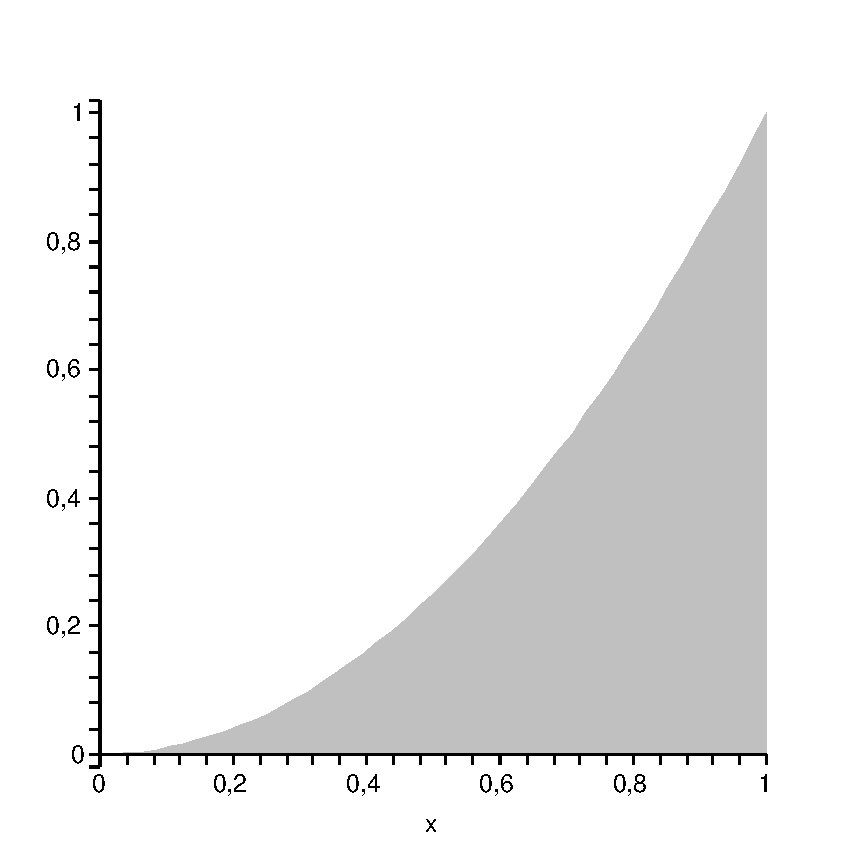
\epsfig{file=Figures/xhoch2int.eps,scale=0.4}
   \caption{Die Fl�che unter der Parabel $x \mapsto x^2$ im Intervall $[0,1]$.}
  \label{fig:xhoch2int.eps}
\end{figure}

Wir k�nnen versuchen, diese Fl�che durch sogenannte
\emph{Treppen-Funktionen} zu approximieren.  Eine Treppen-Funktion ist eine Funktion, die
st�ckweise konstant ist.  Abbildung \ref{fig:xhoch2RiemannRight.eps} auf Seite 
\pageref{fig:xhoch2RiemannRight.eps} zeigt eine Approximation der Funktion $x \mapsto x^2$
durch eine Treppen-Funktion.  In dieser Abbildung haben wir das Intervall $[0,1]$ in 10 gleich
gro�e Teilintervalle aufgeteilt.  Wollen wir im allgemeinen Fall die Fl�che unter eine
Funktion $f$ in einem vorgegebenen Intervall $[a,b]$ berechnen, so 
unterteilen wir das Intervall $[a,b]$ in $n$ Teilintervalle der Form 
\\[0.2cm]
\hspace*{1.3cm}
$\bigl[a + (i-1) \cdot  h, a + i\cdot h \bigr]$ \quad mit $\ds h := \frac{b-a}{n}$ und $i=1,\cdots,n$.
\\[0.2cm]
Um dann die Fl�che berechnen zu k�nnen, approximieren wir diese Fl�che
zum einen durch eine Treppen-Funktion, die oberhalb der zu integrierenden Funktion liegt und zum anderen durch eine
Treppen-Funktion, die unterhalb der zu integrierenden Funktion liegt.  Wir nehmen zur
Vereinfachung zun�chst an, dass die Funktion $f$ monoton steigend ist.
In diesem Fall definieren wir zu einer vorgegebenen Zahl $n$ von Intervallen die obere
Treppen-Funktion $f^\downarrow_{n}(x)$ wie folgt:
\begin{equation}
  \label{eq:treppeOben}
  f^\downarrow_n(x) := f(a + i\cdot h) \quad \mbox{falls}\; 
  x \in  \bigl(a+(i-1)\cdot h,\, a+i\cdot h\bigr)\;\mbox{und}\;i=1,\cdots,n.
\end{equation}
Da wir $f$ als monoton steigend vorausgesetzt haben, gilt 
\\[0.2cm]
\hspace*{1.3cm}
$\forall x \in \bigl( a+(i-1)\cdot h, a+i\cdot h\bigr): f(x) \leq f(a+i\cdot h) = f^\downarrow(x)$,
\\[0.2cm]
die Funktion $f$ liegt also unterhalb der Treppen-Funktion $f^\downarrow$.
Wie die Treppen-Funktion an den Randpunkten der Intervalle $[a+(i-1)\cdot h, a+i\cdot h]$ definiert
wird, ist unwichtig.  Abbildung \ref{fig:xhoch2RiemannRight.eps} zeigt die Funktion 
$f(x) = x^2$ und die zugeh�rige Treppen-Funktion $f^\downarrow_{10}(x)$.  Die Fl�che unter
einer solchen Treppen-Funktion kann leicht berechnet werden:  Schreiben wir
\\[0.2cm]
\hspace*{1.3cm}
$\ds \int_a^b f(x) \,dx$
\\[0.2cm] 
f�r die Fl�che unter einer Funktion $f$ in dem Intervall $[a,b]$, so gilt f�r die
Treppen-Funktion $f^\downarrow_{n}$ offenbar
\begin{equation}
  \label{eq:intOber}
  \int_a^b f^\downarrow_n(x) \,dx = \sum\limits_{i=1}^n f(a+i\cdot h)\cdot h
\end{equation}
denn die Fl�che eines Rechtecks berechnet sich als das Produkt von Breite und H�he.  Die
H�he des Rechtecks im $i$-ten Teilintervall hat den Wert $f(a + i\cdot h)$ und die Breite
des Teilintervalls ist $h$.

\begin{figure}[!t]
  \centering
   \epsfig{file=Figures/xhoch2RiemannRight.eps,scale=0.5}
   \caption{Die Fl�che unter der Parabel $x \mapsto x^2$ im Intervall $[0,1]$.}
  \label{fig:xhoch2RiemannRight.eps}
\end{figure}

Genau wie wir die Fl�che unter der Funktion $f$ von oben approximieren k�nnen, k�nnen wir
diese Fl�che auch von unten approximieren. Die dazu notwendige Treppen-Funktion
$f^\uparrow_n(x)$ definieren wir analog zu Gleichung (\ref{eq:treppeOben})
\begin{equation}
  \label{eq:treppeUnten}
  f^\uparrow_n(x) = f(a + (i-1)\cdot h) \quad \mbox{falls}\; x \in (a+(i-1)\cdot h, a+i\cdot h),
\end{equation}
wir werten also diesmal in jedem Intervall die Funktion $f$ am linken Eckpunkt aus,
denn dort ist die Funktion $f$ am kleinsten, denn wir haben ja vorausgesetzt, dass
die Funktion $f$ monoton steigend ist.
F�r diese Treppen-Funktion berechnet sich die Fl�che also nach der Formel
\begin{equation}
  \label{eq:intUnter}
  \int_a^b f^\uparrow_n(x) \,dx = \sum\limits_{i=1}^{n} f\bigl(a+(i-1)\cdot h\bigr)\cdot h
  = \sum\limits_{i=0}^{n-1} f(a+i\cdot h)\cdot h.
\end{equation}
F�r die Fl�che, die zwischen der Funktion $f$ und der $x$-Achse liegt, haben wir insgesamt
die Absch�tzung
\\[0.2cm]
\hspace*{1.3cm}
$\ds\sum\limits_{i=0}^{n-1} f(a+i\cdot h)\cdot h \leq \int_a^b f(x) \,dx \leq \sum\limits_{i=1}^{n} f(a+i\cdot h)\cdot h$ 
\\[0.2cm]
gefunden.  Die linke Summe bezeichnen wir als \emph{Unter-Summe}, die Summe auf der
rechten Seite der Ungleichungskette nennen wir \emph{Ober-Summe}.
Wir k�nnen hoffen, dass f�r wachsende Werte von $n$ die Werte von Ober-Summe und
Unter-Summe gegen den selben Grenzwert konvergieren.  Dazu berechnen wir zun�chst die
Differenz dieser beiden Summen:
\\[0.2cm]
\hspace*{1.3cm}
$
\begin{array}{cl} 
    & \ds \sum\limits_{i=1}^{n} f(a+i\cdot h)\cdot h - \sum\limits_{i=0}^{n-1} f(a+i\cdot h)\cdot h \\[0.4cm]
 =  & \ds f(a+n\cdot h)\cdot h - f(a)\cdot h  \\[0.1cm]
 =  & \ds \biggl(f\Bigl(a+n\cdot \frac{b-a}{n}\Bigr) - f(a)\biggr)\cdot  \frac{b-a}{n}  \\[0.3cm]
 =  & \ds \Bigl(f(a+ b-a) - f(a)\Bigr)\cdot  \frac{b-a}{n}  \\[0.3cm]
 =  & \ds \Bigl(f(b) - f(a)\Bigr)\cdot  \frac{b-a}{n}  \\[0.3cm]
{\longrightarrow \atop {n \rightarrow \infty}} & 0
\end{array}
$
\\[0.3cm]
Damit ist klar, dass bei einer monoton steigenden Funktion die Ober-Summe f�r eine
wachsende Zahl $n$ von Intervallen gegen den 
selben Wert konvergiert wie die Unter-Summe.  Daher definieren wir
\begin{equation}
  \label{eq:integral}
  \int_a^b f(x) \,dx := \lim\limits_{n\rightarrow \infty} \sum\limits_{i=1}^n f\Bigl(a + i
  \cdot \frac{b-a}{n}\Bigr) \cdot \frac{b-a}{n}
\end{equation}
Diesen Grenzwert nennen wir auch das \emph{Integral} von $f$ in dem Intervall $[a,b]$.
Die so gegebene Definition ist zun�chst nur f�r monoton wachsende Funktionen schl�ssig,
aber es ist offensichtlich, dass das Integral f�r monoton fallende Funktionen auf die
selbe Weise berechnet werden kann.  Ist nun eine Funktion $f$ in dem Intervall $f$ weder
monoton fallend noch monoton steigend, so k�nnen wir versuchen, dass Intervall so in
Teilintervalle aufzuspalten, dass $f$ in jedem Teilintervall monoton fallend oder monoton
steigend ist.  Da wir auf jedem dieser Teilintervalle das Integral nach der Formel 
(\ref{eq:integral}) berechnen k�nnen, k�nnen wir dann auch insgesamt das Integral nach
dieser Formel berechnen.

\exercise
Berechnen Sie das Integral 
\\[0.2cm]
\hspace*{1.3cm}
$\dint{0}{b} x^2\, dx$
\\[0.2cm]
nach der in (\ref{eq:integral}) angegebenen Formel.
\vspace*{0.2cm}

\noindent
\textbf{Hinweis:}  Es gilt
\\[0.2cm]
\hspace*{1.3cm}
$\ds \sum\limits_{i=1}^n i^2 = \frac{n}{6} \cdot (n + 1) \cdot (2 \cdot n + 1)$.
\eox
\pagebreak

\begin{Definition}[Integral]
  Ist $f:[a,b] \rightarrow \mathbb{R}$ eine Funktion, so dass der Grenzwert 
\\[0.2cm]
\hspace*{1.3cm}
$\ds\lim\limits_{n\rightarrow \infty} \sum\limits_{i=1}^n f\Bigl(a + i \cdot  \frac{b-a}{n}\Bigr) \cdot \frac{b-a}{n}$
\\[0.2cm]
existiert, so nennen wir $f$ \emph{integrierbar} und definieren das \emph{Integral} von $f$
in dem Intervall $[a,b]$ als 
  \\[0.2cm]
  \hspace*{1.3cm}
  $\dint{a}{b} f(x) \,dx = 
   \lim\limits_{n\rightarrow \infty} \sum\limits_{i=1}^n f\Bigl(a + i \cdot \frac{b-a}{n}\Bigr) \cdot \frac{b-a}{n}
  $.  \eod
\end{Definition}

\noindent
Der so eingef�hrte Integral-Begriff hat folgende Eigenschaften:
\begin{enumerate}
\item Linearit�t: Sind $f$ und $g$ zwei Funktionen, so dass
      das Integral �ber $f$ bzw.~$g$ in dem Inter\-vall $[a,b]$ definiert ist
      und sind $\alpha,\beta \in\mathbb{R}$,
      so ist auch das Integral der Funktion
      \\[0.2cm]
      \hspace*{1.3cm} $x \mapsto \alpha\cdot f(x) + \beta\cdot g(x)$ \\[0.2cm]
      definiert und es gilt 
      \\[0.2cm]
      \hspace*{1.3cm}
      $\ds\int_a^b \alpha\cdot f(x) + \beta\cdot g(x)\,dx = \alpha\cdot \int_a^b f(x)\,dx + \beta\cdot \int_a^b g(x)\,dx$.
      \\[0.2cm]
      Diese Eigenschaft folgt aus der Tatsache, dass sowohl die Summe als auch das Produkt zweier konvergenter Folgen 
      wieder konvergent sind.
\item Monotonie:  Sind $f$ und $g$ zwei Funktionen, so dass
      das Integral �ber $f$ und  $g$ in dem Intervall $[a,b]$ definiert ist, so gilt: 
      \\[0.2cm]
      \hspace*{1.3cm}
      $\ds\Bigl(\forall x \in [a,b]: f(x) \leq g(x)\Bigr) \;\Rightarrow\;
       \int_a^b f(x)\, dx \,\leq\, \int_a^b g(x)\, dx$.
      \\[0.2cm] 
      Auch diese Eigenschaft folgt aus der entsprechenden Eigenschaft konvergenter Folgen.
\end{enumerate}


\begin{Satz}[Mittelwert-Satz der Integral-Rechnung] \hspace*{\fill} \\
Es sei $f:[a,b] \rightarrow \mathbb{R}$ eine stetige Funktion. Dann existiert ein $\xi \in [a,b]$, so dass gilt:
\\[0.2cm]
\hspace*{1.3cm}
$\ds\int_a^b f(x) \,dx = f(\xi) \cdot  (b - a)$.
\end{Satz}

\noindent
\textbf{Beweis}: Da die Funktion $f$ stetig ist, nimmt $f$ auf dem Intervall $[a,b]$ ein
Minimum und ein Maximum in den Punkten $x_{min}$ und $x_{max}$ an.  Dann gilt 
\\[0.2cm]
\hspace*{1.3cm}
$\forall x \in [a,b]: f\bigl(x_{min}\bigr) \leq f(x) \leq f\bigl(x_{max}\bigr)$.
\\[0.2cm]
Aufgrund der Monotonie des Integral-Operators folgt daraus sofort 
\\[0.2cm]
\hspace*{1.3cm}
$
\begin{array}{cl} 
                & \dint{a}{b} f\bigl(x_{min}\bigr)\, dx \leq \int_a^b f(x)\, dx \leq \int_a^b f\bigl(x_{max}\bigr)\,dx \\[0.3cm]
\Leftrightarrow & \ds f\bigl(x_{min}\bigr) \cdot  (b-a) \leq \int_a^b f(x)\, dx \leq f\bigl(x_{max}\bigr)\cdot (b-a) \\[0.3cm]
\Leftrightarrow & \ds f\bigl(x_{min}\bigr) \leq \frac{1}{b-a} \cdot \int_a^b f(x)\, dx \leq f\bigl(x_{max}\bigr) \\[0.3cm]
\end{array}
$
\\[0.2cm]
Die obige Ungleichungskette zeigt, dass 
\\[0.2cm]
\hspace*{1.3cm}
 $\ds \frac{1}{b-a} \cdot \int_a^b f(x)\, dx\; \in \bigl[f(x_{min}), f(x_{max})\bigr]$ \\[0.2cm]
gilt.  
Aufgrund des Zwischenwert-Satzes f�r stetige Funktionen (Satz \ref{satz:zws-stetig} auf Seite
\pageref{satz:zws-stetig}) nimmt die stetige Funktion $f$ jeden Wert in dem  
Intervall $\bigl[f\bigl(x_{min}\bigr), f\bigl(x_{max}\bigr)\bigr]$ an.  
Also gibt es ein $\xi \in [a,b]$, so dass 
\\[0.2cm]
\hspace*{1.3cm}
$f(\xi) = \ds \frac{1}{b-a} \cdot \int_a^b f(x)\, dx$
\\[0.2cm]
gilt und dass ist �quivalent zu 
\\[0.2cm]
\hspace*{1.3cm}
$\ds f(\xi) \cdot  (b- a) = \int_a^b f(x)\, dx$. \hspace*{\fill} $\Box$
\vspace*{0.3cm}

\noindent
Der Mittelwert-Satz versetzt uns in die Lage, einen Zusammenhang zwischen
Differential-Rechnung und Integral-Rechnung herzustellen.

\begin{Satz}[Ableitung von Integralen] \lb
  \label{satz:ableitungInt}
  Die Funktion $f:[a,b] \rightarrow \mathbb{R}$ sei stetig.  Definieren wir f�r 
  $x \in [a,b]$ die Funktion  $F:[a,b] \rightarrow \mathbb{R}$ durch 
  \\[0.2cm]
  \hspace*{1.3cm}
  $\ds F(x) := \int_a^x f(t)\, dt$,
  \\[0.2cm]
  so ist die Funktion $F$ im Intervall $[a,b]$ differenzierbar und es gilt 
  \\[0.2cm]
  \hspace*{1.3cm} $\df F(x) = f(x)$.
\end{Satz}

\noindent
\textbf{Beweis}: Es gilt
\\[0.3cm]
\hspace*{1.3cm}
$
\begin{array}[t]{cll}  

   &\ds \df F(x) \\[0.3cm]
 = &\ds  \lim\limits_{h\rightarrow 0} \frac{F(x+h) - F(x)}{h} \\[0.3cm]
 = &\ds \lim\limits_{h\rightarrow 0} \ds\frac{\int_a^{x+h} f(t)\, dt - \int_a^x f(t)\, dt}{h} &
      \mbox{nach Definition von $F$} \\[0.3cm]
 = &\ds \lim\limits_{h\rightarrow 0} \ds\frac{1}{h}\int_{x}^{x+h} f(t)\, dt \\[0.5cm]
 = &\ds \lim\limits_{h\rightarrow 0} \ds\frac{1}{h} \cdot  (x+h - x) \cdot   f(\xi_h) &
      \mbox{nach dem Mittelwertsatz f�r ein $\xi_h\in[x, x+h]$} \\[0.5cm]
 = &\ds \lim\limits_{h\rightarrow 0} \ds f(\xi_h) \\[0.3cm]
 = & \ds f(x) & \mbox{wegen $\xi_h \in [x, x+h]$}.
\end{array}
$
\\[0.3cm]
Damit ist die Behauptung bewiesen. \hspace*{\fill} $\Box$

\remark
Der letzte Satz zeigt uns, dass der Differentiations-Operator
\\[0.2cm]
\hspace*{1.3cm}
$\ds\frac{d\,\cdot}{dx} := \left(f \mapsto \frac{df}{dx} \right)$ 
\\[0.2cm]
zu dem Integral-Operator
\\[0.2cm]
\hspace*{1.3cm}
$\ds\int_{a}^x \cdot \;dt := \left(f \mapsto \int_a^x f(t) \, dt\right)$ 
\\[0.2cm]
invers ist: Wenden wir auf eine Funktion zun�chst den
Integral-Operator an und wenden wir dann auf die resultierende Funktion den
Differentiations-Operator an, so erhalten wir wieder die urspr�ngliche Funktion:
\\[0.2cm]
\hspace*{1.3cm}
\colorbox{orange}{\framebox{$\ds \frac{d\;}{dx} \int_a^x f(t)\,dt = f(x)$.}}
\\[0.2cm]
Diese Aussage
l�sst sich im Wesentlichen auch umkehren.  Diese Umkehrung ist der Hauptsatz der Differential- und
Integral-Rechnung.  Bevor wir diesen Satz in Angriff nehmen k�nnen, ben�tigen wir noch eine Definition.


\begin{Definition}[Stamm-Funktion] \lb
Ist $f:[a,b] \rightarrow \mathbb{R}$ eine Funktion, so ist die Funktion 
 $F:[a,b]\rightarrow\mathbb{R}$ 
eine \emph{Stamm-Funktion} von $f$, falls $F$ differenzierbar ist und 
\\[0.2cm]
\hspace*{1.3cm} $\df F(x) = f(x)$
\\[0.2cm]
gilt.  In diesem Fall schreiben wir auch  $\ds F(x) = \int f(x) \, dx$.
Der Ausdruck $\ds\int f(x) \, dx$ wird als \emph{unbestimmtes Integral} bezeichnet. \eod
\end{Definition}



Die Schreibweise $\ds F(x) = \int f(x) \, dx$ ist problematisch, denn die Stamm-Funktion einer
gegebenen Funktion ist nicht eindeutig.  Ist $F(x)$ eine Stamm-Funktion von $f(x)$ und
definieren wir die Funktion $G$ durch $G(x) := F(x) + c$ f�r eine beliebige Konstante $c$,
so ist nat�rlich auch $G(x)$ eine Stamm-Funktion von $f$, denn es gilt
\\[0.2cm]
\hspace*{1.3cm}
$\df G(x) = \df F(x) + \df c = f(x) + 0 = f(x)$.
\\[0.2cm]
Umgekehrt gilt, dass zwei verschiedene Stamm-Funktionen zu einer Funktion $f$ sich nur um
eine Konstante unterscheiden.  Dies sehen wir wie folgt: Angenommen, $F_1$ und $F_2$ seien
zwei Stamm-Funktionen einer Funktion $f$, es gelte also 
\\[0.2cm]
\hspace*{1.3cm}
$\df{F_1}(x) = f(x)$ \quad und \quad $\df{F_2}(x) = f(x)$.
\\[0.2cm]
Dann definieren wir die Funktion $H$ als $H(x) := F_1(x) - F_2(x)$.  Damit gilt
\\[0.2cm]
\hspace*{1.3cm}
$\df H(x) = \df{F_1}(x) - \df{F_2}(x) = f(x) - f(x) = 0$.
\\[0.2cm]
Nach Lemma \ref{lemma:0_ableitung} gibt es nun eine Konstante $c$, so dass $H(x) = c$ gilt.
Wir kommen jetzt zu einem zentralen Ergebnis dieser Vorlesung.

\begin{Satz}[Hauptsatz der Differential- und Integral-Rechnung] \hspace*{\fill} \\
 Die Funktion $f:[a,b] \rightarrow\mathbb{R}$ sei stetig, $F:[a,b] \rightarrow\mathbb{R}$
sei eine Stamm-Funktion von $f$ und es gelte $u,v\in[a,b]$.  Dann gilt
\\[0.2cm]
\hspace*{1.3cm}
\colorbox{orange}{\framebox{$\dint{u}{v} f(x)\,dx = F(v) - F(u)$.}}  
\end{Satz}

\noindent
\textbf{Beweis}: Definieren wir die Funktion $G(x)$ durch 
\\[0.2cm]
\hspace*{1.3cm}
$\ds G(x) := \int_a^x f(t)\, dt$ \quad f�r alle $x\in[a,b]$,
\\[0.2cm]
so besagt Satz \ref{satz:ableitungInt}, dass die Funktion $G$ eine Stamm-Funktion der
Funktion $f$ ist.  Ist nun $F$ eine beliebige weitere Stamm-Funktion von $f$, so haben wir
gerade gesehen, dass die Stamm-Funktionen $G$ und $F$ sich nur um eine Konstante $c$
unterscheiden k�nnen, es gilt also
\\[0.2cm]
\hspace*{1.3cm}
$F(x) = G(x) + c$.
\\[0.2cm]
Damit haben wir 
\\[0.2cm]
\hspace*{1.3cm}
$
\begin{array}[t]{lcl}
  F(v) - F(u) & = & G(v) + c - \bigl(G(u) + c\bigr) \\[0.2cm]
              & = & G(v) - G(u)                     \\[0.2cm]
              & = & \ds\int_a^v f(t)\, dt - \int_a^u f(t)\, dt \\[0.3cm]
              & = & \ds\int_u^v f(t)\, dt. \hspace*{9cm} \Box  
\end{array}
$
\vspace*{0.3cm}

\noindent
Der letzte Satz gibt Anla� zu einer Schreibweise.  F�r eine Funktion $F$  definieren wir
\\[0.2cm]
\hspace*{1.3cm}
$F(x) \Big|_u^v := F(v) - F(u)$.
\\[0.2cm]
Den letzten Satz k�nnen wir eine wichtige Schlussfolgerung ziehen:  Ist $f:[a,b] \rightarrow\mathbb{R}$
eine differenzierbare Funktion, so ist $f$ offenbar eine Stamm-Funktion der Funktion $f'(x)$.
Also gilt:
\begin{equation}
  \label{eq:hauptsatzKorollar}
  \colorbox{orange}{\framebox{$\ds\int_u^v f'(x)\,dx = f(v) - f(u) = f(x)\Big|_u^v$}}
\end{equation}
Dies zeigt uns, dass der Integral-Operator in gewisser Weise zum Differential-Operator invers ist.

\section{Regeln zur Berechnung von Integralen}
Der Hauptsatz der Differential- und Integral-Rechnung erm�glicht es, Regeln zur Berechnung
von Integralen aufzustellen.  Tabelle \ref{tab:integrale} zeigt die Stamm-Funktionen der
wichtigsten Funktionen.  Um diese Tabelle zu verifizieren reicht es aus, die in der rechten
Spalte der Tabelle angegebene Funktion nach $x$ zu differenzieren.
Wir f�hren dies exemplarisch f�r den Eintrag $\ln(x)$ vor.  Es gilt
\\[0.3cm]
\hspace*{1.3cm}
$
\begin{array}[t]{lcll}  
\dfo \bigl( x\cdot \ln(x) - x\bigr) & = & \dfo \bigl( x\cdot \ln(x) \bigr) - \dfo x \\[0.3cm] 
 & = &\ds 1 \cdot  \ln(x) + x \cdot  \frac{1}{x} - 1 & (\mbox{Produkt-Regel}) \\[0.2cm]
 & = &\ds \ln(x) + 1 - 1  \\[0.2cm]
 & = & \ds \ln(x) \\
\end{array}
$
\\[0.3cm]
Damit ist gezeigt, dass $\ds\int \ln(x)\;dx = x\cdot \ln(x) - x$ gilt.  Die �brigen Eintr�ge der
Tabelle k�nnen auf �hnliche Weise verifiziert werden.

\begin{table}[h]
  \centering
  \begin{tabular}[t]{|l|l|}
    \hline
    Funktion $f(x)$ & Stamm-Funktion $\ds \rule[-12pt]{0pt}{30pt}\int\!\! f(x) \, dx$ \\
    \hline
    \hline
    $x^\alpha$ mit $\alpha\not= -1$ & \rule[-12pt]{0pt}{30pt} $\ds \frac{1}{\alpha + 1}\cdot x^{\alpha + 1}$ \\
    \hline
    $\ds \frac{1}{x} $ & \rule[-12pt]{0pt}{30pt} $\ln\bigl(|x|\bigr)$ \\
    \hline
    $\exp(x)$                      & \rule[-6pt]{0pt}{18pt} $\exp(x)$ \\
    \hline
    $\sin(x)$                      & \rule[-6pt]{0pt}{18pt} $-\cos(x)$ \\
    \hline
    $\cos(x)$                      & \rule[-6pt]{0pt}{18pt} $\sin(x)$ \\
    \hline
    $\tan(x) $ & \rule[-6pt]{0pt}{18pt} $-\ln\bigl(|\cos(x)|\bigr)$ \\
    \hline
    $\ln(x)$ & \rule[-6pt]{0pt}{18pt} $x\cdot \ln(x) - x$ \\
    \hline
    $\ds \frac{1}{1+x^2}$ & \rule[-12pt]{0pt}{30pt} $\arctan(x)$ \\
    \hline
    $\ds \frac{1}{\sqrt{1-x^2}} $ & \rule[-14pt]{0pt}{30pt} $\arcsin(x)$ \\
    \hline
    $\ds \frac{1}{\sqrt{1+x^2}} $ & \rule[-14pt]{0pt}{30pt} $ \ln  \left( x+\sqrt {1+{x}^{2}} \right) $ \\
    \hline
    $\arctan(x)$ & \rule[-12pt]{0pt}{30pt} $\ds x\cdot \arctan(x) -\frac{1}{2}\cdot \ln\bigl( 1+{x}^{2} \bigr)$ \\
    \hline
  \end{tabular}
  \caption{Tabelle einiger Integrale}
  \label{tab:integrale}
\end{table}
Bemerkenswert ist vielleicht noch die Stamm-Funktion der Funktion $\ds x \mapsto \frac{1}{x}$:
F�r $x>0$ gilt 
sicher 
\\[0.2cm]
\hspace*{1.3cm}
$\dfo \ln(x) = \frac{1}{x}$
\\[0.2cm]
Au�erdem gilt nach der Ketten-Regel f�r $x < 0$ 
\\[0.2cm]
\hspace*{1.3cm}
$\dfo \ln(-x) = -1 \cdot  \frac{1}{-x} = \frac{1}{x}$.
\\[0.2cm]
Diese beiden Gleichungen k�nnen wir zu 
\\[0.2cm]
\hspace*{1.3cm}
$\dfo \ln\bigl(|x|\bigr) = \frac{1}{x}$
\\[0.2cm]
zusammen fassen und folglich haben wir
\\[0.2cm]
\hspace*{1.3cm}
 $\bint \frac{1}{x}\,dx = \ln\bigl(|x|\bigr)$.
\\[0.2cm]
Wir k�nnen die einzelnen Eintr�ge der Tabelle zwar durch Differenzieren leicht
verifizieren, aber dabei bleibt die Frage offen, wie die Eintr�ge dieser Tabelle gefunden
wurden.  Wir stellen jetzt einige S�tze auf, mit deren Hilfe wir Stamm-Funktionen
gegebener Funktionen berechnen k�nnen.  Wir erhalten diese S�tze indem wir die
Regeln, die wir zur Differenzierung aufgestellt haben, umdrehen.  

\subsection{Die Substitutions-Regel}
Wir beginnen damit, dass wir die Ketten-Regel umstellen.
\\[0.3cm]
\hspace*{1.3cm}
$
\begin{array}[t]{llcll}
            & \dfo h(f(x)) & = & f'(x) \cdot  h'(f(x)) & \mbox{Ketten-Regel} \\[0.3cm]
\Rightarrow & \bint\dfo h(f(x))\, dx & = & \bint f'(x) \cdot  h'(f(x))\, dx  \;+\; c & \mbox{Stamm-Funktion bilden} \\[0.3cm]
\Rightarrow & h(f(x))  & = & \bint f'(x) \cdot  h'(f(x))\, dx \;+\; c   & \mbox{Definition der Stamm-Funktion}. \\[0.3cm]
\end{array}
$
\\[0.3cm]
Nach dem Hauptsatz k�nnen wir hier bei den Integralen Grenzen einsetzen. Dann erhalten wir
\begin{equation}
  \label{eq:subst0}
  \int_a^b f'(x) \cdot  h'(f(x))\, dx  =  h\bigl(f(b)\bigr) - h\bigl(f(a)\bigr)
\end{equation} 
Wir definieren nun $g(x) := h'(x)$.  Dann ist $h$ eine Stamm-Funktion der Funktion $g$, es
gilt also $h(x) = \int g(x)\, dx \,+\, d$ , was wir nach dem Hauptsatz auch als
\begin{equation}
  \label{eq:subst1}
h\bigl(f(b)\bigr) - h\bigl(f(a)\bigr) = \int_{f(a)}^{f(b)} g(x)\,dx  
\end{equation}
schreiben k�nnen.
Ersetzen wir in Gleichung (\ref{eq:subst0})  $h'$
durch $g$ so erhalten wir zusammen mit Gleichung (\ref{eq:subst1})  die \emph{Substitutions-Regel}:
\begin{equation}
  \label{eq:subst}
\colorbox{orange}{\framebox{$\ds\int_a^b f'(x) \cdot  g\bigl(f(x)\bigr)\, dx = \int_{f(a)}^{f(b)} g(x)\, dx$}}.  
\end{equation}
Sie k�nnen sich die Substitutions-Regel mit Hilfe der folgenden suggestiven Pseudo-Ableitung
leicht merken.  Wir gehen aus von dem unbestimmten Integral 
\\[0.2cm]
\hspace*{1.3cm}
$\ds\int g(y)\, dy$.
\\[0.2cm]
Hier f�hren wir die Variablen-Transformation $y = f(x)$ durch. Dann gilt 
\\[0.2cm]
\hspace*{1.3cm}
$\ds \frac{dy}{dx} = f'(x)$
\\[0.2cm]
Wir rechnen nun mit dem Ausdruck $\ds\frac{dy}{dx}$ so, als ob es ein gew�hnlicher Bruch w�re und stellen die
letzte Gleichung nach $dy$ um.  Dann haben wir 
\\[0.2cm]
\hspace*{1.3cm}
$dy = f'(x)\cdot dx$
\\[0.2cm]
Ersetzen wir in dem urspr�nglichen Integral $dy$ durch diesen Ausdruck, so haben wir 
\\[0.2cm]
\hspace*{1.3cm}
$\ds\int g(y)\, dy = \int g\bigl(f(x)\bigr)\cdot f'(x)\, dx$
\\[0.2cm]
Das ist aber genau die Substitutions-Regel f�r unbestimmte Integrale.

\exercise
Berechnen Sie das Integral $\ds \int_0^x \tan(t)\, dt$ mit Hilfe der Substitutions-Regel.  \eox

\solution
Es gilt:
\\[0.2cm]
\hspace*{1.3cm}
$
\begin{array}[t]{lcl}
       \dint{0}{x} \tan(t) \, dt 
 & = & \dint{0}{x} \;\frac{\sin(t)}{\cos(t)}\, dt \\[0.3cm]
 & = & - \dint{0}{x} \;\bigl(- \sin(t)\bigr)\cdot \frac{1}{\cos(t)}\, dt \\[0.6cm]
 & = & - \dint{\cos(0)}{\cos(x)} \;\frac{1}{y}\, dy \\[0.6cm]
 & = & - \Bigl( \ln\bigl(|\cos(x)|\bigr) - \ln\bigl(|\cos(0)|\bigr) \Bigr) \\[0.3cm]
 & = & \ln\bigl(|\cos(0)|\bigr) - \ln\bigl(|\cos(x)|\bigr) \\[0.3cm]
 & = & \ln(1) - \ln\bigl(|\cos(x)|\bigr) \\[0.2cm]
 & = & - \ln\bigl(|\cos(x)|\bigr) 
\end{array}
$
\\[0.2cm]
Damit ist gezeigt, dass die Funktion  $x \mapsto -\ln\bigl(|\cos(x)|\bigr)$ eine Stamm-Funktion der
Funktion $x\mapsto\tan(x)$ ist:
\\[0.2cm]
\hspace*{1.3cm} $\bint\tan(x)\, dx = - \ln\bigl(|\cos(x)|\bigr) + c$.
\\[0.2cm]
Wir zeigen, wie sich die Stamm-Funktion von $\tan(x)$ suggestiver berechnen l��t.  Bei dem
Integral
\\[0.2cm]
\hspace*{1.3cm}
 $\ds\int \frac{\sin(t)}{\cos(t)}\,dt$ 
\\[0.2cm]
 f�hren wir die Variablen-Transformation $x =
\cos(t)$ durch.  Dann gilt
\\[0.2cm]
\hspace*{1.3cm}
 $\ds\frac{dx}{dt} = -\sin(t) \;\Leftrightarrow\; dt = \frac{dx}{-\sin(t)}$.
\\[0.2cm]
Ersetzen wir in dem Integral
\\[0.2cm]
\hspace*{1.3cm}
 $\ds\int \frac{\sin(t)}{\cos(t)}\,dt$ \quad den Ausdruck $dt$ durch \quad  $\ds\frac{dx}{-\sin(t)}$ 
\\[0.2cm]
und $\cos(t)$ durch $x$,  so erhalten wir
\\[0.2cm]
\hspace*{1.3cm} 
$\ds \int \frac{\sin(t)}{\cos(t)}\,dt \;=\; \int
\frac{\sin(t)}{x}\cdot \frac{dx}{-\sin(t)} \;=\; - \int \frac{1}{x}\, dx = -\ln(|x|) =
-\ln\bigl(|\cos(t)|\bigr) $.  
\\[0.2cm]
Das Rechnen mit den \emph{infinitesimalen} Gr��en $dx$ und $dt$ ist
offensichtlich intuitiver als die formale Anwendung der Substitutions-Regel.  \qed


\exercise
Berechnen Sie das Integral
\\[0.2cm]
\hspace*{1.3cm}
$\bint\frac{x}{1 + x^2} \, dx$
\\[0.2cm]
mit  Hilfe der Substitutions-Regel.  \eox


\subsection{Partielle Integration}
Als n�chstes �berlegen wir, wie wir aus der Produkt-Regel der Differential-Rechnung
eine Regel zur Berechnung von Integralen gewinnen k�nnen.  Es gilt
\\[0.2cm]
$
\begin{array}[t]{llcll}
                & \dfo \Bigl(f(x)\cdot g(x)\Bigr)  & = & f'(x)\cdot  g(x) + f(x) \cdot  g'(x) &\mbox{(Umstellen)} \\[0.3cm]
\Leftrightarrow & f'(x) \cdot  g(x) & = & \dfo \Bigl(f(x)\cdot g(x)\Bigr) - f(x) \cdot  g'(x) &\mbox{(Stamm-Funktion)} \\[0.3cm]
\Leftrightarrow & \ds \int f'(x)\cdot  g(x)\,dx & = & \bint\dfo \Bigl(f(x)\cdot g(x)\Bigr)\,dx - \int f(x) \cdot  g'(x)\,dx \\[0.3cm]
\end{array}
$
\\[0.2cm]
Die Stamm-Funktion von $\dfo\Bigl( f(x)\cdot g(x) \Bigr)$ ist nat�rlich $f(x)\cdot g(x)$, also haben wir
\begin{equation}
  \label{eq:partInt0}
 \colorbox{orange}{\framebox{$\ds\int f'(x)\cdot  g(x)\,dx =  \ds f(x)\cdot g(x) - \int f(x) \cdot  g'(x)\,dx$}}
\end{equation}
gefunden. Diese Gleichung setzt die Stamm-Funktionen von $f'(x)\cdot  g(x)$
und $f(x) \cdot  g'(x)$ in Beziehung: Die Stamm-Funktion der ersten Funktion kann auf die
Stamm-Funktion der zweiten Funktion zur�ck gef�hrt werden.
Die Regel zur partiellen Integration l��t sich nicht nur f�r die Berechnung der
Stamm-Funktion eines Produkts einsetzen, sondern sie wird auch benutzt um die Integrale von
Umkehr-Funktionen zu bestimmen.  Als Beispiel zeigen wir, wie sich das Integral der 
Funktion $\ln(x)$ mittels partieller Integration bestimmen l��t.
\\[0.3cm]
\hspace*{1.3cm}
$
\begin{array}[t]{lcl}
 \bint\ln(x)\,dx & = &  \bint1\cdot \ln(x)\,dx \\[0.2cm]
                 & = &  x\cdot \ln(x) - \bint x\cdot \dfo \ln(x)\,dx \\[0.3cm]
                 & = &  x\cdot \ln(x) - \bint x\cdot \frac{1}{x}\,dx \\[0.3cm]
                 & = &  x\cdot \ln(x) - \bint 1\,dx \\[0.2cm]
                 & = &  x\cdot \ln(x) - x \\[0.2cm]
\end{array}
$

\exercise
Berechnen Sie die Stamm-Funktion $\ds\int \arctan(x)\,dx$.  \eox

\subsection{Das Integral von Umkehr-Funktionen$^*$}
Wir zeigen noch einen anderen Weg, mit dem das Integral der Umkehr-Funktion einer Funktion
berechnet werden kann.  Es sei also eine Funktion $f:[a,b] \rightarrow\mathbb{R}$ geben,
die eine Umkehr-Funktion hat.  Wir setzen zur Vereinfachung jetzt voraus, dass die
Funktion $f$ monoton steigend ist, wenn $f$ monoton fallend ist, liegen die Dinge analog.
Die Umkehr-Funktion von $f$ sei die Funktion
\\[0.2cm]
\hspace*{1.3cm}
 $g:\bigl[f(a), f(b)\bigl]
\rightarrow\mathbb{R}$, \quad f�r alle $x\in[a,b]$ gilt also $g\bigl(f(x)\bigr) = x$.  
\\[0.2cm]
Analog gilt dann f�r alle $y\in\bigl[f(a),f(b)\bigr]$ die Gleichung
$f\bigl(g(y)\bigr) = y$. Abbildung \ref{fig:umkehr.eps} zeigt die Funktion.  Durch
Spiegelung an der Winkelhalbierung geht die Funktion $f$ in die Umkehr-Funktion �ber,
wenn wir also die $y$-Achse als $x$-Achse ansehen, zeigt die Abbildung die Umkehr-Funktion.
Wir betrachten jetzt die Fl�che des Rechtecks, dessen linke unter Ecke
im Ursprung des Koordinaten-Systems liegt und dessen rechte obere Ecke die Koordinaten
$\bigl\langle b,f(b)\bigr\rangle$ hat.  Dieses Rechtecks hat den Fl�cheninhalt $b\cdot f(b)$.
Diese Fl�che setzt sich aus drei Teilen zusammen, die in der Figur unterschiedlich markiert
sind.
\begin{enumerate}
\item Links unten findet sich ein kleines Rechteck, das mit diagonalen Streifen markiert
      ist.  Die linke untere Ecke dieses Rechtecks liegt ebenfalls im Ursprung des
      Koordinaten-Systems, die rechte obere Ecke hat die Koordinaten $\bigl\langle a,f(a)\bigr\rangle$.
      Damit hat dieses Rechteck die Fl�che $a\cdot f(a)$.
\item Die vertikal schraffierte Fl�che ist die Fl�che unter der Kurve $f(x)$ und ist
      folglich gegeben durch das Integral
      \\[0.2cm]
      \hspace*{1.3cm} $\ds \int_a^b f(x)\, dx$.
\item Die horizontal schraffierte Fl�che ist die Fl�che unter der Kurve $g(y)$ der
      Umkehr-Funktion   und ist daher gegeben durch 
      \\[0.2cm]
      \hspace*{1.3cm} $\ds \int_{f(a)}^{f(b)} g(y)\, dy$.
\end{enumerate}
Nat�rlich ist die gesamte Fl�che des Rechtecks die Summe aller drei Teile, es gilt also
\begin{equation}
  \label{eq:umkehr0}
  b\cdot f(b) = a\cdot f(a) + \int_a^b f(t)\, dt + \int_{f(a)}^{f(b)} g(t)\, dt 
\end{equation}


\begin{figure}[!h]
  \centering
  \framebox{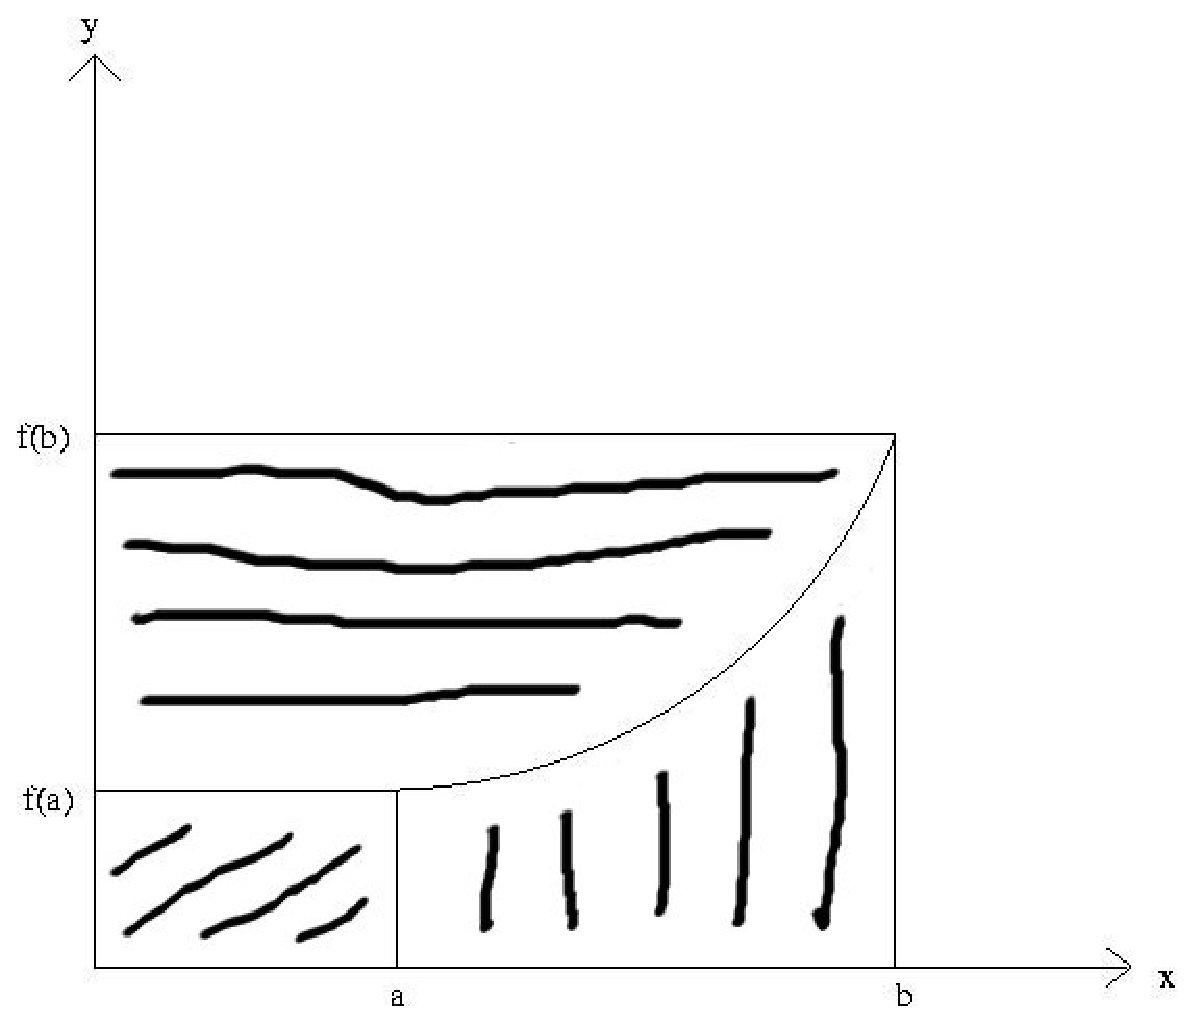
\epsfig{file=Figures/umkehr,scale=0.4}} 
  \caption{Die Funktion $f:[a,b] \rightarrow\mathbb{R}$}
  \label{fig:umkehr.eps}
\end{figure}

Ersetzen wir in dieser Gleichung  $b$ durch $x$ und stellen die Gleichung nach dem ersten
Integral um, so erhalten wir
\begin{equation}
  \label{eq:umkehr}
  \int_a^x f(t)\, dt = x\cdot f(x) - a\cdot f(a) - \int_{f(a)}^{f(x)} g(t)\, dt 
\end{equation}
Sind wir nur an Stamm-Funktionen interessiert, so k�nnen wir den konstanten Term $a\cdot f(a)$
weglassen.  Dann schreibt sich die letzte Gleichung als
\begin{equation}
  \label{eq:umkehr1}
  \int f(x)\, dx = x\cdot f(x) - G\bigl(f(x)\bigr) \quad \mbox{mit}\;\; G(x) := \int g(x)\, dx. 
\end{equation}

\example 
Wir betrachten die Funktion $f(x) = \ln(x)$ mit der Umkehr-Funktion 
$g(x) = \exp(x)$.  Wegen $\ds\int \exp(x)\,dx = \exp(x)$ gilt 
\\[0.3cm]
\hspace*{1.3cm}
$\bint \ln(x) = x\cdot \ln(x) - \exp\bigl(\ln(x)\bigr) = x\cdot \ln(x) - x$. \eox

\subsection{Berechnung der Fl�che eines Kreises}
Wir zeigen, wie sich der Fl�chen-Inhalt eines Kreises berechnen l��t.  Ein Kreis vom Radius 1 kann
nach dem Satz des Pythagoras  in der Koordinaten-Ebene durch die Relation $x^2 + y^2 = 1$ dargestellt werden.
L�sen wir diese Gleichung nach $x$ auf, so wird der Kreis durch die beiden Funktionen $x
\mapsto \sqrt{1 - x^2}$
und $x \mapsto -\sqrt{1 - x^2}$ f�r $x\in[-1,1]$ beschrieben.  Wir beschr�nken
uns nun auf den Viertelkreis im ersten Quadranten der Koordinaten-Ebene.  Die Fl�che
dieses Viertelkreises ist durch das Integral 
\\[0.2cm]
\hspace*{1.3cm}
$I := \dint{0}{1} \sqrt{1 - x^2\,}\, dx$
\\[0.2cm]
gegeben, dass wir nun berechnen.  Zun�chst f�hren wir die Koordinaten-Transformation
$x = \sin(t)$ durch.  Dann erhalten wir
\\[0.2cm]
\hspace*{1.3cm}
$\ds\frac{dx}{dt} = \cos(t)$, \quad also $dx = \cos(t)\cdot dt$.
\\[0.2cm]
Wegen $0=\sin(0)$ und $1 = \sin(\pi/2)$ haben wir
\\[0.2cm]
\hspace*{1.3cm}
$\ds I = \int_0^{\frac{\pi}{2}} \sqrt{1 - \sin^2(t)\,} \cdot \cos(t)\, dt = \int_0^{\frac{\pi}{2}} \cos(t) \cdot \cos(t)\, dt$.
\\[0.2cm]
Dieses Integral versuchen wir nun mit partieller Integration zu vereinfachen.  Wir setzen
in Gleichung \ref{eq:partInt0} $f'(t) := \cos(t)$ und $g(t) = \cos(t)$.  Wegen $f(t) =
\sin(t)$ und $g'(t) = -\sin(t)$ erhalten wir dann
\\[0.2cm]
\hspace*{1.3cm}
$\ds I = \sin(t)\cdot \cos(t)\bigg|_0^{\frac{\pi}{2}} + \int_0^{\frac{\pi}{2}}\sin(t)\cdot\sin(t)\,dt
   = \int_0^{\frac{\pi}{2}}\sin^2(t)\,dt$
\\[0.2cm]
Damit haben wir jetzt 
\\[0.2cm]
\hspace*{1.3cm}
$\ds I = \int_0^{\frac{\pi}{2}}\cos^2(t)\,dt =  \int_0^{\frac{\pi}{2}}\sin^2(t)\,dt$
\\[0.2cm]
Daraus folgt \\
\hspace*{1.3cm}
$
\begin{array}[t]{llcl}
\Leftrightarrow & 2\cdot I & = & \ds \int_0^{\frac{\pi}{2}}\cos^2(t)\,dt + \int_0^{\frac{\pi}{2}}\sin^2(t)\,dt \\[0.5cm]
\Leftrightarrow & 2\cdot I & = & \ds \int_0^{\frac{\pi}{2}}\bigl(\cos^2(t)\,dt + \sin^2(t)\bigr)\,dt \\[0.5cm]
\Leftrightarrow & 2\cdot I & = & \ds \int_0^{\frac{\pi}{2}} 1 \,dt \\[0.5cm]
\Leftrightarrow & 2\cdot I & = & \ds t\; \Big|_0^{\frac{\pi}{2}}  \\[0.4cm]
\Leftrightarrow & 2\cdot I & = & \ds \frac{\pi}{2}  \\[0.4cm]
\Leftrightarrow & I & = & \ds \frac{\pi}{4}
\end{array}
$
\\[0.3cm]
Damit haben wir f�r die Fl�che eines Viertelkreises den Wert $\ds\frac{\pi}{4}$ gefunden, der
ganze Kreis hat also die Fl�che $\pi$.

\section{Berechnung der Bogenl�nge}
Gelegentlich tritt das Problem auf, die L�nge der Strecke zu berechnen, die durch einen
Funktions-Graphen beschrieben wird.  Geht es darum, die Bogenl�nge des Graphen der Funktion 
$f:[a,b] \rightarrow\mathbb{R}$ in dem Intervall $[a,b]$ zu berechnen, so zerlegen wir das
Intervall in $[a,b]$ in $n$ Teilintervalle der L�nge 
\\[0.2cm]
\hspace*{1.3cm}
$\ds h = \frac{b - a}{n}$.
\\[0.2cm]
Das Teilst�ck des Graphen, das von dem Punkt $\bigl\langle x, f(x) \bigr\rangle$  zu dem Punkt 
$\bigl\langle x + h, f(x+h) \bigr\rangle$ kann f�r kleine Werte von $h$ n�herungsweise
durch die Sekante von dem  Punkt $\bigl\langle x, f(x) \bigr\rangle$  zu dem Punkt
$\bigl\langle x + h, f(x+h) \bigr\rangle$  approximiert werden.  Nach dem Satz des
Pythagoras hat diese Sekante die L�nge
\\[0.2cm]
\hspace*{1.3cm}
$ds = \sqrt{h^2 + \bigl(f(x+h) - f(x)\bigr)^2\,}$.
\\[0.2cm] 
Nach Definition der Ableitung von $f$ gilt f�r kleine Werte von $h$
\\[0.2cm]
\hspace*{1.3cm}
$\ds \frac{f(x+h) - f(x)}{h} \approx f'(x)$.
\\[0.2cm]
Also haben wir 
\\[0.2cm]
\hspace*{1.3cm}
$f(x+h) - f(x) \approx f'(x) h$.
\\[0.2cm]
Setzen wir diesen Wert in der obigen Formel f�r ein, so erhalten wir
\\[0.2cm]
\hspace*{1.3cm}
$\ds ds \approx \sqrt{h^2 + \bigl(f'(x) \cdot h\bigr)^2\,} = \sqrt{1 + \Bigl(\frac{d\/f}{dx}\Bigr)^2\,}\cdot h$.
\\[0.2cm]
Die L�nge $l$ des gesamten Funktions-Graphen erhalten wir, wenn wir diesen Ausdruck von $a$ bis $b$
aufintegrieren: 
\\[0.2cm]
\hspace*{1.3cm}
\colorbox{orange}{\framebox{$\ds l = \dint{a}{b} \sqrt{1 + \Bigl(\frac{df}{dx}\Bigr)^2\,} dx$}}.

\example
Wir berechnen die L�nge $l$ des Kreisbogens, der durch die Funktion $f:[0,1] \rightarrow\mathbb{R}$ mit
\\[0.2cm]
\hspace*{1.3cm}
$f(x) = \sqrt{1 - x^2}$
\\[0.2cm]
definiert ist.  Anschaulich sollte diese L�nge ein Viertel des Umfangs eines Kreises mit Radius $1$ betragen.
Es gilt
\\[0.2cm]
\hspace*{1.3cm}
$\ds\frac{d\/f}{dx} = \frac{1}{2} \cdot \frac{-2 \cdot x}{\sqrt{1 - x^2}} = 
                  \frac{- x}{\sqrt{1 - x^2}}
$.
\\[0.2cm]
Also haben wir f�r die L�nge
\\[0.2cm]
\hspace*{1.3cm}
$
\begin{array}[t]{lcl}
l & = & \dint{0}{1} \sqrt{1 + \frac{x^2}{1 - x^2}\,}\, dx \\[0.5cm]
  & = & \dint{0}{1} \frac{1}{\sqrt{1 - x^2\,}}\, dx
\end{array}
$
\\[0.2cm]
An dieser Stelle wenden wir die Substitutions-Regel
\\[0.2cm]
\hspace*{1.3cm}
$\dint{a}{b} f'(x) \cdot  g\bigl(f(x)\bigr)\, dx = \dint{f(a)}{f(b)} g(x)\, dx$
\\[0.2cm]
an, wobei wir 
\\[0.2cm]
\hspace*{1.3cm}
$f(x) := \sin(x)$,\quad $g(x) := \ds \frac{1}{\sqrt{1 - x^2\,}}$, 
\quad $a := 0$ \quad und \quad $b := \ds \frac{\pi}{2}$
\\[0.2cm]
setzen. Wegen
\\[0.2cm]
\hspace*{1.3cm}
$f'(x) = \cos(x)$, \quad $\sin(0) = 0$ \quad und \quad $\sin(\pi/2) = 1$
\\[0.2cm]
folgt dann
\\[0.2cm]
\hspace*{1.3cm}
$
\begin{array}[t]{lcl}
l & = & \dint{0}{\pi/2} \cos(x) \cdot \frac{1}{\sqrt{1 - \sin^2(x)}}\, dx  \\[0.6cm]
  & = & \dint{0}{\pi/2} \cos(x) \cdot \frac{1}{\cos(x)}\, dx  \\[0.6cm]
  & = & \dint{0}{\pi/2} 1\, dx  \\[0.6cm]
  & = &  x \Bigl|_0^{\pi/2}  \\[0.4cm]
  & = &  \frac{\pi}{2}  
\end{array}
$
\\[0.2cm]
und das ist genau der Umfang eines Viertel-Kreises. \eod

\exercise
Berechnen Sie die Bogenl�nge der Parabel $x \mapsto x^2$ im Intervall $[0,1]$. 
\eod 

\section{Uneigentliche Integrale}
Ist bei dem Ausdruck $\int_a^b f(x)\,dx$ die Funktion $f$ an einer der Intervall-Grenzen
nicht definiert, so bezeichnen wir den Ausdruck als uneigentliches Integral.  Wir
betrachten nur den Fall, dass die Funktion $f$ nur in dem halboffenen Intervall $(a, b]$
definiert ist, w�hrend $f$  in dem Punkt $a$ nicht definiert sein soll.  Beispielsweise
ist die Funktion $x \mapsto \frac{1}{\sqrt{x}}$ im Punkt $x=0$ nicht definiert.  In diesem
Fall definieren wir 
\\[0.2cm]
\hspace*{1.3cm}
$\ds \int_a^b f(x)\, dx := \lim\limits_{h\rightarrow 0 \atop h > 0} \int_{a+h}^b f(x)\, dx$.
\\[0.2cm]
Wir betrachten als Beispiel das Integral der Funktion $\ds x \mapsto \frac{1}{\sqrt{x}}$ in
dem Intervall $[0,1]$.  Es gilt
\\[0.2cm]
\hspace*{1.3cm}
$\ds \int_0^1 \frac{1}{\sqrt{x}}\, dx 
 = \lim\limits_{h\rightarrow 0 \atop h >  0} \int_{h}^1 \frac{1}{\sqrt{x}}\, dx
 = \lim\limits_{h\rightarrow 0 \atop h >  0} 2\cdot\sqrt{x}\; \Big|_h^1
 = \lim\limits_{h\rightarrow 0 \atop h >  0} 2\cdot\sqrt{1} - 2\cdot\sqrt{h} = 2$.
\\[0.2cm]
Ein anderer Fall liegt vor, wenn eine der Integrations-Grenzen den Wert Unendlich hat.
Wir betrachten nur den Fall $b= \infty$.  In diesem Fall definieren wir
\\[0.2cm]
\hspace*{1.3cm}
$\ds \int_a^\infty f(t)\, dt := \lim\limits_{x\rightarrow \infty} \int_{a}^x f(t)\, dt$.
\\[0.2cm]
Wir betrachten als Beispiel die Funktion $\ds x \mapsto \frac{1}{x^2}$ in dem Intervall
$[1,\infty)$. Es gilt
\\[0.2cm]
\hspace*{1.3cm}
$\ds \int_1^\infty \frac{1}{t^2}\, dt = 
\lim\limits_{x\rightarrow \infty} \int_{1}^x \frac{1}{t^2}\, dt =
\lim\limits_{x\rightarrow \infty} - \frac{1}{t}\;\Big|_1^x =
\lim\limits_{x\rightarrow \infty} - \frac{1}{x} + \frac{1}{1}  = 1
$.
\\[0.2cm]
Indem wir Reihen und uneigentliche Integrale in Beziehung setzen, k�nnen wir unter
Umst�nden leicht sehen, dass eine Reihe konvergiert, denn es gilt der folgende Satz.


\begin{Satz}[Integral-Vergleichskriterium]
Es sei $f:[1,\infty) \rightarrow\mathbb{R}_+$ eine monoton fallende Funktion.  Dann gilt
\\[0.2cm]
\hspace*{1.3cm}
$\ds \lim\limits_{n \rightarrow \infty} \sum\limits_{i=1}^n f(i)$ existiert \quad g.d.w. \quad
$\ds \lim\limits_{x \rightarrow \infty} \int\limits_1^x f(t)\,dt$ existiert.  
\end{Satz}

\noindent
\textbf{Beweis}:
F�r alle $i\in \mathbb{N}$ mit $i>1$ und alle $x \in [i-1,i]$ gelten die Ungleichungen
\\[0.2cm]
\hspace*{1.3cm}
$i-1 \leq x$ \quad und \quad $x \leq i$.
\\[0.2cm]
Da die Funktion $f$ monoton fallend ist, folgt daraus
\\[0.2cm]
\hspace*{1.3cm}
$f(i) \leq f(x)$ \quad und \quad $f(x) \leq f(i-1)$.
\\[0.2cm]
Aus der Monotonie des Integral-Operators folgt nun
\\[0.2cm]
\hspace*{1.3cm}
$\ds\int\limits_{i-1}^{i} f(i)\, dx \leq \int\limits_{i-1}^{i} f(x)\, dx$
\quad und \quad
$\ds \int\limits_{i-1}^i f(x)\, dx \leq \int\limits_{i-1}^i f(i-1)\, dx$
\\[0.2cm]
Das Integral �ber die konstanten Funktionen $x \mapsto f(i)$ bzw.~$x \mapsto f(i-1)$
liefert nur den konstanten Funktions-Wert multipliziert mit der L�nge des Intervalls, die nat�rlich 1
ist.  Also haben wir die Ungleichungen
\\[0.2cm]
\hspace*{1.3cm}
$\ds f(i) \leq \int\limits_{i-1}^{i} f(x)\, dx$
\quad und \quad
$\ds\int_{i-1}^{i} f(x)\, dx \leq f(i\!-\!1)$
\\[0.2cm]
gezeigt.  Summieren wir diese Ungleichungen f�r alle $i$ aus der Menge $\{2,\cdots,n\}$,
  so erhalten wir 
\\[0.2cm]
\hspace*{1.3cm}
$\ds\sum\limits_{i=2}^n f(i) \leq \dint{1}{n} f(x)\, dx$
\quad und \quad
$\dint{1}{n} f(x)\, dx \leq \sum\limits_{i=2}^n f(i\!-\!1)$
\\[0.2cm]
Bei der ersten Ungleichung addieren wir noch $f(1)$, bei der zweiten Ungleichung ersetzen
wir die Summations-Variable $i$ durch $i+1$ und erhalten:
\\[0.2cm]
\hspace*{1.3cm}
$\ds \sum\limits_{i=1}^n f(i) \leq f(1) + \dint{1}{n} f(x)\, dx$
\quad und \quad
$\dint{1}{n} f(x)\, dx \leq \sum\limits_{i=1}^{n-1} f(i)$
\\[0.2cm]
Falls nun das Integral $\int_{1}^\infty f(x)\, dx$ existiert, so gilt
\\[0.2cm]
\hspace*{1.3cm}
$\ds \sum\limits_{i=1}^{n} f(i) \leq f(1) + \int\limits_{1}^n f(x)\, dx \leq f(1) + \int\limits_{1}^\infty f(x)\, dx$
\\[0.2cm]
Damit ist dann die Folge 
\\
\hspace*{1.3cm}
$\ds \biggl(\sum\limits_{i=1}^{n}  f(i)\biggr)_{n\in\mathbb{N}}$ 
\\ 
monoton und beschr�nkt, folglich konvergent.  Existiert umgekehrt der Grenzwert
$\ds \sum\limits_{i=1}^{\infty} f(i)$, so  ist aufgrund der zweiten Ungleichung auch die Folge
\\[0.3cm]
\hspace*{1.3cm}
$\ds \biggl(\int_{1}^n f(x)\, dx\biggr)_{n\in\mathbb{N}}$
\\[0.3cm]
beschr�nkt.  Da diese Folge au�erdem monoton ist, folgt die Konvergenz. \hspace*{\fill} $\Box$
\vspace*{0.3cm}

\noindent
\textbf{Beispiel}: Wir betrachten das Integral 
\\[0.2cm]
\hspace*{1.3cm}
$\ds \int\limits_{1}^\infty \frac{1}{x^\alpha}\, dx$ \quad f�r $\alpha > 0$.
\\[0.2cm]
Falls $\alpha \not= 1$ ist,  gilt 
\\[0.2cm]
\hspace*{1.3cm}
$
\begin{array}[t]{clcl}  
  &I(\alpha) & := & \ds \int_{1}^\infty \frac{1}{t^\alpha}\, dt  \\[0.3cm]
= & \ds \lim\limits_{x \rightarrow \infty} \int_1^x \frac{1}{t^\alpha}\, dt 
& = & \ds \lim\limits_{x \rightarrow \infty} \frac{t^{1-\alpha}}{1-\alpha} \,\bigg|_1^x \\[0.5cm]
= & \ds \lim\limits_{x \rightarrow \infty} \frac{x^{1-\alpha}-1}{1-\alpha}.
\end{array}
$
\\[0.3cm]
Im Falle $\alpha = 1$ haben wir
\\[0.2cm]
\hspace*{1.3cm}
$I(\alpha) = \ln(x)$.
\\[0.2cm]
Nun h�ngt alles davon ab, ob $\alpha < 1$, $\alpha = 1$ oder 
 $\alpha > 1$ ist.
\begin{enumerate}
\item Falls $\alpha < 1$ ist, haben wir $1-\alpha>0$ und damit gilt
      \\[0.2cm]
      \hspace*{1.3cm}
      $\ds I(\alpha) = \lim\limits_{x \rightarrow \infty} \frac{x^{1-\alpha}-1}{1-\alpha} = \infty$
      \\[0.2cm]
      Also konvergiert die Summe 
      \\[0.2cm]
      \hspace*{1.3cm}
      $\ds \sum\limits_{i=1}^{\infty} \frac{1}{i^\alpha}$
      \\[0.2cm]
      in diesem Fall nicht.
\item Falls $\alpha = 1$ ist, gilt
      \\[0.2cm]
      \hspace*{1.3cm}
      $I(1) = \lim\limits_{x \rightarrow \infty} \dint{1}{x}\; \frac{1}{t}\, dt 
            =  \lim\limits_{x \rightarrow \infty} \ln(x)  = \infty
      $
      \\[0.2cm]
      Im letzten Schritt haben wir hier ausgenutzt, dass
      \\[0.2cm]
      \hspace*{1.3cm}
      $\lim\limits_{x \rightarrow \infty} \ln(x) = \infty$
      \\[0.2cm]
      gilt.  Das folgt daraus, dass die Funktion $x \mapsto \ln(x)$ einerseits monoton steigend ist und
      dass andererseits 
      \\[0.2cm]
      \hspace*{1.3cm}
      $\ln\bigl(\exp(n)\bigr) = n$ \quad f�r alle $n \in \mathbb{N}$  
      \\[0.2cm]
      gilt, denn die letzte Gleichung zeigt, dass die Funktion $x \mapsto \ln(x)$ beliebig gro� wird. 

      Insgesamt k�nnen wir nun aus dem Integral-Vergleichskriterium folgern, dass die
      harmonische Reihe divergiert:
      \\[0.2cm]
      \hspace*{1.3cm}
      $\ds\sum\limits_{i=1}^{\infty} \frac{1}{i} = \infty$.
\item Falls $\alpha > 1$ ist, haben wir $1-\alpha<0$ und damit gilt
      \\[0.2cm]
      \hspace*{1.3cm}
      $\ds I(\alpha) = \lim\limits_{x \rightarrow \infty} \frac{x^{1-\alpha}-1}{1-\alpha} = \frac{1}{\alpha-1}$
      \\[0.2cm]
      In diesem Fall konvergiert also die Summe 
      \\[0.2cm]
      \hspace*{1.3cm}
      $\ds \sum\limits_{i=1}^{\infty} \frac{1}{i^\alpha}$.
\end{enumerate}

\exercise
Untersuchen Sie mit Hilfe des Integral-Vergleichskriteriums, ob die
Reihe 
\\[0.2cm]
\hspace*{1.3cm}
$\ds \sum\limits_{n=1}^\infty \frac{1}{n\cdot (n+1)}$ 
\qquad
konvergiert.  \eox


\section{Numerische Integration$^*$}
Die Gleichung $x = \cos(x)$ haben wir zwar numerisch l�sen k�nnen, aber wir waren nicht in
der Lage, einen algebraischen Ausdruck f�r die L�sung anzugeben.  Auch bei der Integration
von Funktionen ist es nicht immer m�glich, einen algebraischen Ausdruck f�r die
Stamm-Funktion einer Funktion anzugeben.  Beispielsweise konnte Liouville 
(Joseph Liouville, 1809 -- 1882) beweisen, dass das
unbestimmte Integral
\\[0.2cm]
\hspace*{1.3cm}
$\int \exp(-x^2)\, dx$
\\[0.2cm]
nicht auf die uns bisher bekannten Funktionen zur�ck gef�hrt werden kann \cite{rosenlicht:72}.  F�r die
praktische Berechnung von Integralen ben�tigen wir daher numerische Methoden.

\subsection{Die Trapez-Regel}
Die wohl naheliegenste Methode besteht darin, die zu integrierende Funktion st�ckweise
linear zu interpolieren und dann das zur berechnende Integral durch das Integral der
st�ckweise linearen Funktion zu approximieren.
Ist das Integral $\int_a^b f(t)\,dt$ zu berechnen, so wird zun�chst das Intervall $[a,b]$
in $n$ gleich gro�e Teilintervalle zerlegt.  Das $i$-te Teilintervall ist $[a+(i-1)\cdot h,
a+i\cdot h]$ mit $h := \frac{b-a}{n}$ und $i=1,\cdots,n$.
Wir setzen $x_i := a+i\cdot h$.
Innerhalb des $i$-ten Teilintervalls wird die Funktion $f(x)$ dann durch die Gerade 
\\[0.2cm]
\hspace*{1.3cm}
$\ds g(x) = f\bigl(x_{i-1}\bigr)\cdot \frac{x - x_i}{x_{i-1} - x_i} + f\bigl(x_{i}\bigr)\cdot \frac{x - x_{i-1}}{x_{i} - x_{i-1}}$
\\[0.2cm]
approximiert.  Das Integral �ber $g(x)$ im Intervall $[x_{i-1}, x_i]$ ist dann
$$
\begin{array}[t]{cl}
  &  \dint{x_{i-1}}{x_i} g(x)\, dx \\[0.5cm]
= &  \dint{x_{i-1}}{x_i} f\bigl(x_{i-1}\bigr)\cdot \frac{x - x_i}{x_{i-1} - x_i} + f\bigl(x_{i}\bigr)\cdot \frac{x - x_{i-1}}{x_{i} - x_{i-1}}\,dx \\[0.5cm]
= &  \ds\frac{f\bigl(x_{i-1}\bigr)}{x_{i-1} - x_i} \cdot  \int_{x_{i-1}}^{x_i} (x - x_i)\,dx +
                  \frac{f\bigl(x_{i}\bigr)}{x_{i} - x_{i-1}} \cdot  \int_{x_{i-1}}^{x_i} (x - x_{i-1})\,dx \\[0.5cm]
= &  \ds\frac{f\bigl(x_{i-1}\bigr)}{x_{i-1} - x_i} \cdot \frac{1}{2} \cdot (x - x_i)^2 \Big|_{x_{i-1}}^{x_i}  +
                  \frac{f\bigl(x_{i}\bigr)}{x_{i} - x_{i-1}} \cdot \frac{1}{2} \cdot (x - x_{i-1})^2 \Big|_{x_{i-1}}^{x_i} \\[0.5cm]
= &  \ds-\frac{f\bigl(x_{i-1}\bigr)}{x_{i-1} - x_i} \cdot \frac{1}{2} \cdot (x_{i-1} - x_i)^2   +
                   \frac{f\bigl(x_{i}\bigr)}{x_{i} - x_{i-1}} \cdot \frac{1}{2} \cdot (x_i - x_{i-1})^2  \\[0.5cm]
= &  \ds \frac{1}{2} \cdot f\bigl(x_{i-1}\bigr) \cdot (x_i - x_{i-1}) +
     \frac{1}{2} \cdot f\bigl(x_{i}\bigr)   \cdot (x_i - x_{i-1})    \\[0.5cm]
= &  \ds \frac{1}{2} \cdot  \Bigl(f\bigl(x_{i}\bigr) + f\bigl(x_{i-1}\bigr)\Bigr) \cdot  (x_{i} - x_{i-1}) 
\end{array}
$$
Die letzte Formel l��t sich geometrisch deuten, denn der Ausdruck 
\\[0.2cm]
\hspace*{1.3cm}
$\frac{1}{2} \cdot  \bigl(f(x_{i}) + f(x_{i-1})\bigr) \cdot  (x_{i} - x_{i-1})$
\\[0.2cm]
beschreibt gerade die Fl�che eines Trapezes mit der Breite $h = x_i - x_{i-1}$ und  Seiten
der L�nge $f(x_i)$ und $f(x_{i-1})$. Daher wird dieses Verfahren zur Berechnung eines Integrals auch als 
\emph{Trapez-Regel} bezeichnet.
Um das Integral �ber das gesamte Intervall $[a,b]$ zu berechnen,
m�ssen wir die Integrale �ber die einzelnen Intervalle lediglich aufsummieren.  Wir erhalten dann 
$$
\begin{array}[t]{lcl}
 \dint{a}{b} f(x)\,dx & \approx & \ds
       \sum\limits_{i=1}^n \frac{1}{2} \cdot \bigl(f(x_i) + f(x_{i-1})\bigr) \cdot (x_i-x_{i-1})  
       \\[0.5cm]
 & = & \ds
       \sum\limits_{i=1}^n \frac{1}{2} \cdot \bigl(f(a+i\cdot h) + f(a+(i-1)\cdot h)\bigr) \cdot  h  \\[0.5cm]
 & = & \ds
       \biggl(\frac{1}{2}\cdot f(a) \;+\; \sum\limits_{i=1}^{n-1} f\Bigl(a+i\cdot \frac{b-a}{n}\Bigr)\;+\;\frac{1}{2}\cdot f(b)\biggr) \cdot  \frac{b-a}{n}  \\[0.5cm]
\end{array}
$$
Abbildung \ref{fig:trapezoidal.eps} auf Seite \pageref{fig:trapezoidal.eps} zeigt die
numerische Berechnung des Integrals $\int_0^1 \exp(x^2)\,dx $ mit Hilfe der Trapez-Regel.
In diesem Fall ist $n=3$.
F�hren wir die Berechnung tats�chlich aus, so erhalten wir die N�herung 
\\[0.2cm]
\hspace*{1.3cm}
$\dint{0}{1} \exp(-x^2)\,dx \approx 0.7399864752\cdots$.
\\[0.2cm]
Der exakte Wert ist $0.7468241328$, unter Ber�cksichtigung der Tatsache, dass wir $n=3$
gew�hlt haben ist die N�herung also gar nicht so schlecht.   Erh�hen wir $n$ auf den Wert 
$300$, so erhalten wir mit der Trapez-Regel die N�herung $0.7468234519$, der Fehler ist
dann also kleiner als $10^{-6}$.  Im n�chsten Satz geben wir eine theoretische Analyse des
Fehlers.

\begin{figure}[!h]
  \centering
   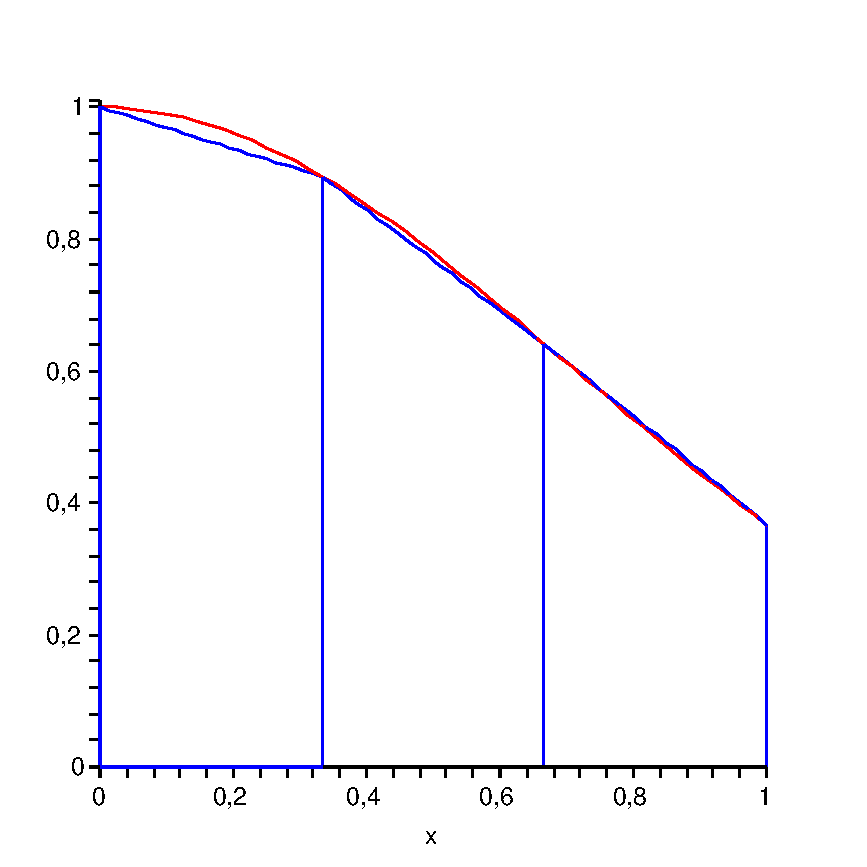
\epsfig{file=Figures/trapezoidal.eps,scale=0.6}
   \caption{Berechnung des Integrals  $\int_0^1 \exp(-x^2)\, dx$ mit Hilfe der Trapez-Regel.}
  \label{fig:trapezoidal.eps}
\end{figure}

\begin{Satz}
  Ist die Funktion $f:[a,b]\rightarrow \mathbb{R}$ zweimal differenzierbar, gilt
  \\[0.2cm]
  \hspace*{1.3cm}
  $\bigl|f^{(2)}(x)\bigr| \leq K$ \quad f�r alle $x\in[a,b]$
  \\[0.2cm]
  und definieren wir gem�� der Trapez-Regel 
  \\[0.2cm]
  \hspace*{1.3cm}
  $\ds I_{\mbox{\scriptsize Trapez}} := \biggl(\frac{1}{2}\cdot f(a) \;+\; \sum\limits_{i=1}^{n-1} f\Bigl(a+i\cdot \frac{b-a}{n}\Bigr)\;+\;\frac{1}{2}\cdot f(b)\biggr) \cdot  \frac{b-a}{n}$
  \\[0.2cm]
  so kann der Unterschied zwischen dem exakten Integral und der N�herung $I_{\mbox{\scriptsize Trapez}}$
  wie folgt abgesch�tzt werden:
  \\[0.2cm]
  \hspace*{1.3cm}
  $\ds \left| \int_a^b f(x)\,dx - I_{\mbox{\scriptsize Trapez}} \right| \;\leq\; 
   \frac{K}{12}\cdot  \frac{(b-a)^3}{n^2}$
\end{Satz}

\noindent
\textbf{Beweis}: Bei der Ableitung der Trapez-Regel haben wir $f(x)$ durch ein lineares
Polynom interpoliert.  Nach Satz \ref{satz:interpolationsFehler} gilt f�r den Unterschied
zwischen $f(x)$ und dem interpolierenden Polynom $p(x)$ vom Grad $n$
\\[0.2cm]
\hspace*{1.3cm}
  $\ds f(x) - p(x) = \frac{f^{(n+1)}(\xi)}{(n+1)!} \cdot  \prod\limits_{i=0}^{n}(x-x_i)$.
\\[0.2cm]
Dabei ist $\xi$ ein nicht n�her bekannter Wert aus dem Intervall $[a,b]$.
Bei linearer Interpolation ist $n=1$ und also haben wir
\\[0.2cm]
\hspace*{1.3cm}
  $\ds f(x) - p(x) = \frac{f^{(2)}(\xi)}{2} \cdot  (x-x_{i-1})\cdot (x-x_i)$.
\\[0.2cm]
Aufgrund der Voraussetzung �ber die zweite Ableitung von $f(x)$ haben wir also
\begin{equation}
  \label{eq:intError1}
  |f(x) - p(x)| \leq \frac{K}{2} \cdot  |(x-x_{i-1})\cdot (x-x_i)|  
\end{equation}
In dem Intervall $[x_{i-1},x_i]$ gilt $x-x_{i-1} \geq 0$ und $x-x_i \leq 0$,
also haben wir
\\[0.2cm]
\hspace*{1.3cm}
 $|(x-x_{i-1})\cdot (x-x_i)| = -(x-x_{i-1})\cdot (x-x_i)$.
\\[0.2cm]
Integrieren wir die Ungleichung \ref{eq:intError1} in dem Intervall $[x_{i-1},x_i]$, so
erhalten wir 
\\[0.3cm]
\hspace*{1.3cm}
$
\begin{array}[t]{cl}
      & \ds  \left|\int_{x_{i-1}}^{x_i} f(x)\,dx - \int_{x_{i-1}}^{x_i}p(x)\,dx\right| \\[0.5cm]
 \leq & \ds  \int_{x_{i-1}}^{x_i} \bigl|f(x)\,dx - p(x)\bigr|\,dx \\[0.5cm]
 \leq & \ds \frac{K}{2} \cdot  \int_{x_{i-1}}^{x_i} \bigl|(x-x_{i-1})\cdot (x-x_i)\bigr|\,dx  \\[0.5cm]
 \leq & \ds -\frac{K}{2} \cdot  \int_{x_{i-1}}^{x_i} (x-x_{i-1})\cdot (x-x_i)\,dx  \\[0.5cm]
 =    & \ds -\frac{K}{2} \cdot  \frac{-1}{6} \cdot  (x_i-x_{i-1})^3\\[0.3cm]
 =    & \ds \frac{K}{12} \cdot  (x_i-x_{i-1})^3
\end{array}
$
\\[0.2cm]
Diese Ungleichung gilt nun f�r jedes $i=1,\cdots,n$.  Summieren wir diese Ungleichungen
f�r alle Intervalle auf, so erhalten wir 
\\[0.2cm]
\hspace*{1.3cm}
$
\begin{array}[t]{lcl}  
\ds \left| \int_a^b f(x)\,dx - I_{\mbox{\scriptsize Trapez}} \right|
& \leq & \ds \sum\limits_{i=1}^n \frac{K}{12} \cdot  (x_i-x_{i-1})^3 \\[0.5cm]
& \leq & \ds \sum\limits_{i=1}^n \frac{K}{12} \cdot  \Bigl(\frac{b-a}{n}\Bigr)^3 \\[0.5cm]
& \leq & \ds n \cdot  \frac{K}{12} \cdot  \Bigl(\frac{b-a}{n}\Bigr)^3  \\[0.5cm]
& \leq & \ds \frac{K}{12} \cdot  \frac{(b-a)^3}{n^2} \\[0.5cm]
\end{array}
$
\\[0.2cm]
Falls wir also die Zahl der Intervalle verzehnfachen, sinkt der Fehler auf ein Hundertstel.
\hspace*{\fill} $\Box$
\vspace*{0.3cm}

\exercise
Berechnen Sie, in wieviele Teilintervalle das Intervall $[0,1]$
aufgeteilt werden muss, wenn das Integral
\\[0.2cm]
\hspace*{1.3cm}
$\ds \int_0^1 e^{-x^2}\, dx$
\\[0.2cm]
mit Hilfe der Trapez-Regel mit einer Genauigkeit von $10^{-6}$ berechnet werden soll. \eod


\subsection{Die Simpson'sche Regel}
Anstatt die zu integrierende Funktion $f$ durch ein lineares Polynom zu interpolieren,
k�nnen wir $f$ auch durch ein Polynom zweiten Grades interpolieren.  Wir brauchen dann
nat�rlich drei St�tzstellen. Daher integrieren wir jetzt nicht mehr �ber ein Intervall
$[x_{i-1},x_i]$, sondern nehmen statt dessen das Intervall $[x_{i-1},x_{i+1}]$ und
benutzen $x_{i-1}$, $x_i$ und $x_{i+1}$ als St�tzstellen.
Die Funktion $f(x)$ approximieren wir in dem Intervall mit der Methode von Lagrange nach
der Formel
\\[0.2cm]
\hspace*{1.3cm}
$
\begin{array}[t]{lcl}
p(x) & = & \ds f(x_{i-1})\cdot \frac{(x-x_i)\cdot (x-x_{i+1})}{(x_{i-1}-x_i)\cdot (x_{i-1}-x_{i+1})}  \\[0.5cm]
     & + & \ds f(x_{i})\cdot \frac{(x-x_{i-1})\cdot (x-x_{i+1})}{(x_{i}-x_{i-1})\cdot (x_{i}-x_{i+1})}  \\[0.5cm]
     & + & \ds f(x_{i+1})\cdot \frac{(x-x_{i-1})\cdot (x-x_{i})}{(x_{i+1}-x_{i-1})\cdot (x_{i+1}-x_{i})}
\end{array}$
\\[0.2cm]
Setzen wir hier $x_{i-1}= x_i-h$ und $x_{i+1}= x_i+h$ und
integrieren dann $p(x)$ in dem Intervall $[x_{i}-h,x_{i}+h]$, so erhalten wir mit Hilfe von \textsl{SymPy} das Ergebnis 
% x[i-1] := x[i] - h;
% x[i+1] := x[i] + h;
% p(x) := f[i-1] * (x - x[i])   * (x - x[i+1]) / ( (x[i-1] - x[i]  ) * (x[i-1] - x[i+1]) ) +
%         f[i]   * (x - x[i-1]) * (x - x[i+1]) / ( (x[i]   - x[i-1]) * (x[i]   - x[i+1]) ) +
%         f[i+1] * (x - x[i-1]) * (x - x[i])   / ( (x[i+1] - x[i-1]) * (x[i+1] - x[i]  ) );
% IntKeppler := int( p(x), x = x[i-1] .. x[[i+1] );
\\[0.2cm]
\hspace*{1.3cm}
$\ds \int_{x_{i-1}}^{x_{i+1}} p(x)\,dx = \frac{1}{6}\cdot \bigl(f(x_{i-1}) + 4 \cdot  f(x_i) + f(x_{i+1})\bigr)\cdot (x_{i+1}-x_{i-1})$
\\[0.2cm]
Unterteilen wir das Intervall $[a,b]$ lediglich in zwei Teilintervalle $[a,\frac{a+b}{2}]$
und $[\frac{a+b}{2},b]$, so k�nnen wir die obige Formel direkt verwenden.  Wir erhalten
dann die \emph{Kepler'sche Fa�regel} (Johannes Kepler, 1571 -- 1630).
\begin{equation}
  \label{eq:keplerFass}
  \int_a^b f(x)\,dx \approx \frac{1}{6} \cdot \Bigl( f(a) + 4 \cdot f\Bigl(\frac{a+b}{2}\Bigr) + f(b)\Bigr)\cdot (b-a)
\end{equation}
Berechnen wir das Integral $\int_0^1 \exp(-x^2)\, dx$ mit dieser Regel, so erhalten wir 
$0.7471804290$ und der Fehler ist bereits kleiner als $4 \cdot 10^{-4}$.

Unterteilen wir das Intervall $[a,b]$ in $n$ Intervalle und ist dar�ber hinaus $n$ eine
gerade Zahl, so k�nnen wir die Regel \ref{eq:keplerFass} jeweils auf die beiden  benachbarten
Intervalle $[x_{2\cdot i},x_{2\cdot i+1}]$ und $[x_{2\cdot i+1},x_{2\cdot i+2}]$ anwenden,
wobei der Index $i$ �ber alle Elemente der Menge $\{0,\cdots,(n-1)/2\}$ l�uft.
Setzen wir $h:=\frac{b-a}{n}$ und $x_i := a + i\cdot h$, so erhalten wir
die Formel 
\begin{equation}
  \label{eq:intSimpson}  
\begin{array}[t]{lcl}
 \ds \int_a^b f(x)\,dx 
& \approx & \ds\frac{h}{3}\cdot \sum\limits_{i=0}^{(n-1)/2} \Bigl( f(x_{2\cdot i}) + 4\cdot f(x_{2\cdot i+1}) + f(x_{2\cdot i+2}) \Bigr) \\[0.3cm]
& = & \ds\frac{h}{3}\cdot \biggl(f(x_0) \;+\; 4\cdot \sum\limits_{i=0}^{(n-1)/2} f(x_{2\cdot i+1}) \;+\;
                                                          2\cdot \sum\limits_{i=1}^{(n-1)/2} f(x_{2\cdot i}) \;+\; f(x_n)\biggr) \\[0.3cm]
\end{array}
\end{equation}
Die obige Formel tr�gt den Namen Simpson'sche Regel (Thomas Simpson, 1710 -- 1761).
Falls die Funktion $f$ insgesamt viermal differenzierbar ist und falls dar�ber hinaus 
die vierte Ableitung von $f$ der Ungleichung 
\\[0.2cm]
\hspace*{1.3cm}
$|f^{(4)}(x)| \leq K$
\\[0.2cm]
gen�gt, so l��t sich der Fehler, der bei der Verwendung der Simpson'schen Regel entsteht, durch
\\[0.2cm]
\hspace*{1.3cm}
$\frac{K}{180}\cdot \frac{(b-a)^5}{n^4}$
\\[0.2cm]
absch�tzen.  Verdoppeln wir die Zahl $n$ der Intervalle, so verkleinert sich der Fehler
also um das 16-fache! W�hlen wir beispielswiese $n=20$ und berechen das Integral
$\int_0^1 \exp(-x^2)\, dx$, so erhalten wir den Wert
$0.746824183$ und der Fehler ist kleiner als $10^{-7}$.
\vspace*{0.3cm}

\renewcommand{\labelenumi}{(\alph{enumi})}
\exercise
\begin{enumerate}
\item Berechnen Sie mit Hilfe der Kepler'schen Fa�-Regel eine Approximation 
      f�r das Integral 
      \\[0.2cm]
      \hspace*{1.3cm}$\ds \int_0^{\frac{1}2} \sin(x)\, dx$.
\item Geben Sie eine m�glichst genaue Absch�tzung f�r den Approximations-Fehler.
\item Vergleichen Sie ihr Ergebnis mit dem exakten Wert. \eod
\end{enumerate}
\pagebreak

\exercise
Gegenstand dieser Aufgabe ist die numerische Berechnung der Summe
\\[0.2cm]
\hspace*{1.3cm}
 $\ds \sum\limits_{k=1}^\infty \frac{1}{k^2}$.
\\[0.2cm]
Gehen  Sie zur Berechnung dieser Summe in folgenden Schritten vor.
\begin{enumerate}
\item Approximieren Sie die Rest-Summe $\sum\limits_{k=n}^\infty \frac{1}{k^2}$ 
      durch ein geeignetes Integral.

      \textbf{Hinweis}: Es gilt $\ds f(k) = \int_{k-\frac{1}{2}}^{k+\frac{1}{2}} f(k) \, dt \approx \int_{k-\frac{1}{2}}^{k+\frac{1}{2}} f(t) \, dt$.
\item Berechnen Sie eine obere Absch�tzung f�r den Approximations-Fehler,
      den Sie bei der Integration in Teil (a) erhalten.
      
      \textbf{Hinweis}: Sch�tzen Sie die auftretenden Summen durch Integrale nach oben ab.
\item Berechnen Sie, wir gro� Sie $n$ w�hlen m�ssen, damit der Approximations-Fehler
      kleiner als $10^{-6}$ bleibt.
\item Geben Sie nun einen N�herungs-Wert f�r die Summe $\sum\limits_{k=1}^\infty \frac{1}{k^2}$ an,
      der sich von dem exakten \\[-0.2cm]
      Ergebnis um weniger als $10^{-6}$ unterscheidet.
\end{enumerate}
\renewcommand{\labelenumi}{(\arabic{enumi})}


%%% Local Variables: 
%%% mode: latex
%%% TeX-master: "analysis"
%%% End: 

\chapter[Die Zahlen $\pi$ und $e$ sind irrational]{Die Kreiszahl $\pi$ und die Euler'sche Zahl $e$ sind irrational}
In diesem Kapitel zeigen wir, dass sowohl die Kreiszahl $\pi$, die als Fl�che eines Kreises mit dem Radius 1
definiert ist, als auch die Euler'sche Zahl $e$, die als Grenzwert der Reihe
\\[0.2cm]
\hspace*{1.3cm}
$\exp(1) := \sum\limits_{k=0}^\infty \bruch{1}{k!}$
\\[0.2cm] 
festgelegt ist, irrational sind.  Da der Nachweis der Irrationalit�t von $e$ einfacher ist, beginnen wir
damit.

\section{Die Euler'sche Zahl $e$ ist irrational}
Nach Definition von $e$ gilt
\\[0.2cm]
\hspace*{1.3cm}
$e = \sum\limits_{k=0}^\infty \bruch{1}{k!}$.
\\[0.2cm]
F�r alle $n \in \mathbb{N}$ definieren wir die $n$-te Partial-Summe $s_n$ als
\\[0.2cm]
\hspace*{1.3cm}
$s_n := \sum\limits_{k=0}^n \bruch{1}{k!}$.
\\[0.2cm]
Als n�chstes definieren wir f�r alle nat�rlichen Zahlen $n \in \mathbb{N}$ den $n$-ten Rest
\\[0.2cm]
\hspace*{1.3cm}
$r_n := e - s_n = \sum\limits_{k=0}^\infty \bruch{1}{k!} - \sum\limits_{k=0}^n \bruch{1}{k!} 
                = \sum\limits_{k=n+1}^\infty \bruch{1}{k!}
$
\\[0.2cm]
Offenbar gilt
\begin{equation}
  \label{eq:e_irrational1}
  0 < r_n,
\end{equation}
denn der $n$-te Rest $r_n$ enth�lt auf jeden Fall den Term $\frac{1}{(n+1)!}$ und der ist positiv.  
Wir wollen nun den $n$-ten Rest $r_n$ nach oben hin absch�tzen.  Dazu ben�tigen wir zun�chst die folgende
Absch�tzung, die f�r alle $k > n + 1$ g�ltig ist:
\\[0.2cm]
\hspace*{1.3cm}
$
\begin{array}[t]{llcl}
                & \bruch{(n+1)!}{k!} & < & \bruch{1}{(n+1)^{k-(n+1)}}  \\[0.4cm]
\Leftrightarrow & \bruch{k!}{(n+1)!} & > & (n+1)^{k-(n+1)}             \\[0.4cm]
\Leftrightarrow & \underbrace{(n+2) \cdot (n+3) \cdot {\dots} \cdot (k-1) \cdot k}_{\mbox{$k-(n+1)$ Faktoren}} & > & 
                  \underbrace{(n+1) \cdot {\dots} \cdot (n+1)}_{\mbox{$k-(n+1)$ Faktoren}} \\[0.4cm]
\end{array}
$
\\[0.2cm]
Die letzte Ungleichung ist richtig, denn die Faktoren auf der linken Seite haben die Form
$(n + 1) + i$ mit $i \in \{1, \cdots, k-(n+1)\}$ und offenbar gilt
\\[0.2cm]
\hspace*{1.3cm}
$(n+1) + i > n+1$ \quad f�r $i \in \{1, \cdots, k-(n+1)\}$,
\\[0.2cm]
so dass zu jedem Faktor in dem Produkt auf der linken Seite ein kleinerer Faktor auf der rechten Seite
korrespondiert.  Falls $k = (n+1)$ ist, gilt
\\[0.2cm]
\hspace*{1.3cm}
$\bruch{(n+1)!}{k!} = \bruch{1}{(n+1)^{k-(n+1)}} = 1$,
\\[0.2cm]
was man unmittelbar durch Einsetzen best�tigen kann.  Wir haben also insgesamt Folgendes gezeigt:
\begin{equation}
  \label{eq:e_irrational2}
 \bruch{(n+1)!}{k!} < \bruch{1}{(n+1)^{k-(n+1)}}  \quad \mbox{f�r alle $k > n+1$}
\end{equation}
und f�r $k = n + 1$ haben wir die Gleichheit beider Seiten.
Nun gilt f�r alle $n \in \mathbb{N}$ mit $n \geq 1$ die folgende Ungleichungs-Kette:
\\[0.2cm]
\hspace*{1.3cm}
$
\begin{array}[t]{lcll}
r_n & = & \sum\limits_{k=n+1}^\infty \bruch{1}{k!}                                      \\[0.2cm]
    & = & \bruch{1}{(n+1)!} \cdot \sum\limits_{k=n+1}^\infty \bruch{(n+1)!}{k!}         \\[0.5cm]
    & < & \bruch{1}{(n+1)!} \cdot \sum\limits_{k=n+1}^\infty \bruch{1}{(n+1)^{k-(n+1)}} 
        & (\mbox{nach Gleichung (\ref{eq:e_irrational2})})                                \\[0.5cm]
    & = & \bruch{1}{(n+1)!} \cdot \sum\limits_{k=0}^\infty \bruch{1}{(n+1)^{k}}    
        & (\mbox{Index-Verschiebung})                                                     \\[0.5cm]
    & = & \bruch{1}{(n+1)!} \cdot \bruch{1}{1 - \frac{1}{n+1}}                    
        & (\mbox{geometrische Reihe})                                                    \\[0.8cm]
    & = & \bruch{1}{(n+1)!} \cdot \bruch{1}{\frac{n + 1 - 1}{n+1}}                    
        & (\mbox{Hauptnenner})                                                            \\[0.8cm]
    & = & \bruch{1}{(n+1)!} \cdot \bruch{n+1}{n}                    
        &                                                                               \\[0.5cm]
    & = & \bruch{1}{n! \cdot n}                     
        &                                                                               \\[0.5cm]
\end{array}
$
\\[0.2cm]
Multiplizieren wir die resultierende Ungleichung mit $n!$, so sehen wir, dass
\\[0.2cm]
\hspace*{1.3cm}
$n! \cdot r_n < \bruch{1}{n}$ 
\\[0.2cm]
gilt.
Fassen wir diese Gleichung zusammen mit der Gleichung (\ref{eq:e_irrational1}), so haben wir insgesamt
\begin{equation}
  \label{eq:e_irrational3}
  0 < n! \cdot r_n < \bruch{1}{n} \quad \mbox{falls $n \geq 1$ ist.}
\end{equation}
Damit ist aber klar, dass der Ausdruck $n! \cdot r_n$ f�r $n \geq 1$ keine nat�rliche Zahl sein kann.

\begin{Theorem}
  Die Eulersche Zahl $e$ ist irrational.
\end{Theorem}

\proof
Wir nehmen an, dass $e$ rational ist.  Dann gibt es nat�rliche Zahlen $p,q \in \mathbb{N}$ mit
$q \geq 1$ und
\\[0.2cm]
\hspace*{1.3cm}
$e = \bruch{p}{q}$.
\\[0.2cm]
Wir betrachten den Ausdruck $q! \cdot r_q = q! \cdot (e - s_q)$ und setzten dort f�r $e$ den Wert $\ds\frac{p}{q}$ ein:
\\[0.2cm]
\hspace*{1.3cm}
$q! \cdot r_q = q! \cdot \Bigl(\bruch{p}{q} - \sum\limits_{k=0}^q \bruch{1}{k!}\Bigr)  
              = \displaystyle (q-1)! \cdot p - \sum\limits_{k=0}^q \bruch{q!}{k!} \in \mathbb{Z}
$,
\\[0.2cm]
denn $(q-1)! \cdot p$ ist auf jeden Fall eine nat�rliche Zahl und f�r $k \leq q$ hat der Ausdruck
$\frac{q!}{k!}$ die Form
\\[0.2cm]
\hspace*{1.3cm}
$\bruch{q!}{k!} = \bruch{1 \cdot 2 \cdot {\dots} \cdot k \cdot (k + 1) \cdot (k + 2) \cdot {\dots} \cdot (q-1) \cdot q}{1 \cdot
  2 \cdot {\dots} \cdot k} 
   = (k + 1) \cdot (k + 2) \cdot {\dots} \cdot (q-1) \cdot q$
\\[0.2cm]
und das ist ebenfalls eine nat�rliche Zahl.  Damit haben wir aber einen Widerspruch, denn die Aussagen
\\[0.2cm]
\hspace*{1.3cm}
$\ds 0 < q! \cdot r_q < \frac{1}{q}$  \quad und \quad $q! \cdot r_q \in \mathbb{Z}$ 
\\[0.2cm]
sind unvereinbar.  \qed


\section{Die Kreiszahl $\pi$ ist irrational$^*$}
Zur Vorbereitung des Beweises ben�tigen wir das folgende Lemma.
\begin{Lemma}
Die Funktion $f:\mathbb{R} \rightarrow \mathbb{R}$ sei beliebig oft differenzierbar. Dann gilt 
f�r alle nat�rlichen Zahlen $n$
\\[0.2cm]
\hspace*{0.8cm}
$\dint{0}{{\pi}} f(x) \cdot \sin(x)\, dx = 
  \sum\limits_{k=0}^n (-1)^k \cdot \bigl(f^{(2k)}(\pi) + f^{(2k)}(0)\bigr) + 
  (-1)^{n+1} \cdot \dint{0}{\pi} f^{(2n+2)}(x) \cdot \sin(x)\, dx
$.
\end{Lemma}

\proof
Zur Abk�rzung definieren wir
\\[0.2cm]
\hspace*{1.3cm}
$I := \dint{0}{{\pi}} f(x) \cdot \sin(x)\, dx$ 
\\
und 
\\
\hspace*{1.3cm}
$\ds S_n := \sum\limits_{k=0}^n (-1)^k \cdot \bigl(f^{(2k)}(\pi) + f^{(2k)}(0)\bigr) + 
  (-1)^{n+1} \cdot \dint{0}{\pi} f^{(2n+2)}(x) \cdot \sin(x)\, dx
$.
\\[0.2cm]
Die Behauptung
\\[0.2cm]
\hspace*{1.3cm}
$I = S_n$
\\[0.2cm]
wird nun durch Induktion nach $n$ bewiesen.  Dabei werden  wir sowohl im Induktions-Anfang als auch
im Induktions-Schritt zwei partielle Integrationen durchf�hren.  
\begin{enumerate}
\item[I.A.:] $n=0$.
     
     Nach Definition von $I$ gilt
     \\[0.2cm]
     \hspace*{1.3cm}
     $I = \dint{0}{\pi} f(x) \cdot \sin(x)\, dx$
     \\[0.2cm]
     Wir integrieren partiell und setzen $u(x) = f(x)$ und $v'(x) = \sin(x)$.
     Dann gilt $u'(x) = f'(x)$ und $v(x) = -\cos(x)$.  Also haben wir
     \\[0.2cm]
     \hspace*{1.3cm}
     $I = - f(x) \cdot \cos(x) \Bigr|_0^\pi + \dint{0}{\pi} f'(x) \cdot \cos(x)$.
     \\[0.2cm]
     F�r den ersten Summanden auf der rechten Seite dieser Gleichung finden wir
     \\[0.2cm]
     \hspace*{1.3cm}
     $  - f(x) \cdot \cos(x) \Bigr|_0^\pi = - f(\pi) \cdot \cos(\pi) + f(0) \cdot \cos(0)
      = f(\pi) + f(0)$.
     \\[0.2cm]
     Um das verbleibende Integral zu berechnen f�hren wir eine erneute partielle Integration durch, bei
     der wir diesmal $u(x) = f'(x)$ und $v'(x) = \cos(x)$ setzen.  Dann gilt $u'(x) = f^{(2)}(x)$ und
     $v(x) = \sin(x)$.  Wegen 
     \\[0.2cm]
     \hspace*{1.3cm}
     $\sin(\pi) = \sin(0) = 0$
     \\[0.2cm]
     finden wir damit f�r das Integral $I$ den Wert
     \\[0.2cm]
     \hspace*{1.3cm}
     $I = f(\pi) + f(0) - \dint{0}{\pi} f^{(2)}(x) \cdot \sin(x)\, dx$.
     \\[0.2cm]
     Auf der anderen Seite haben wir
     \\[0.2cm]
     \hspace*{1.3cm}
     $
     \begin{array}[t]{lcl}
       S_0 & = & \ds \sum\limits_{k=0}^0 (-1)^k \cdot \bigl(f^{(2k)}(\pi) + f^{(2k)}(0)\bigr) + 
                  (-1)^{0+1} \cdot \dint{0}{\pi} f^{(2\cdot 0+2)}(x) \cdot \sin(x)\, dx           \\[0.5cm]
           & = & (-1)^0 \cdot \bigl(f^{(0)}(\pi) + f^{(0)}(0)\bigr)  
                  - \dint{0}{\pi} f^{(2)}(x) \cdot \sin(x)\, dx           \\[0.5cm]
           & = & f(\pi) + f(0) - \dint{0}{\pi} f^{(2)}(x) \cdot \sin(x)\, dx           \\[0.2cm]
           & = & I.
     \end{array}
     $
\item[I.S.:] $n \mapsto n + 1$
     
     Zur Abk�rzung definieren wir
     \\[0.2cm]
     \hspace*{1.3cm}
     $J_n = \dint{0}{\pi} f^{(2n+2)}(x) \cdot \sin(x)\, dx$
     \\[0.2cm]
     Wir berechnen $J_n$ durch partielle Integration und setzen $u(x) := f^{(2n+2)}(x)$ und
     $v'(x) := \sin(x)$.  Dann haben wir $u'(x) = f^{(2n+3)}(x)$ und $v(x) = -\cos(x)$.
     Das liefert
     \\[0.2cm]
     \hspace*{1.3cm}
     $J_n = - f^{(2n+2)}(x) \cdot \cos(x)\Bigr|_0^\pi + \dint{0}{\pi} f^{(2n+3)}(x) \cdot \cos(x)\, dx$.
     \\[0.2cm]
     Wegen $\cos(\pi) = -1$ und $\cos(0) = 1$ vereinfacht sich der erste Summand auf der rechten Seite
     wie folgt:
     \\[0.2cm]
     \hspace*{1.3cm}
     $- f^{(2n+2)}(x) \cdot \cos(x)\Bigr|_0^\pi =  f^{(2n+2)}(\pi) + f^{(2n+2)}(0)$.
     \\[0.2cm]
     Das auf der rechten Seite der obigen Gleichung verbleibende Integral berechnen wir durch eine
     weitere partielle Integration.  Diesmal setzen wir $u(x) = f^{(2n+3)}(x)$ und 
     $v'(x) = \cos(x)$.  Dann haben wir $u'(x) = f^{(2n+3)}(x)$ und $v(x) = \sin(x)$ und f�r das Integral
     finden wir
     \\[0.2cm]
     \hspace*{1.3cm}
     $
     \begin{array}[t]{lcl}
            \dint{0}{\pi} f^{(2n+3)}(x) \cdot \cos(x)\, dx  
      & = & f^{(2n+3)}(x) \cdot \sin(x)\Bigr|_0^\pi - \dint{0}{\pi} f^{(2n+4)}(x) \cdot \sin(x)\, dx  \\[0.4cm]
      & = &  - \dint{0}{\pi} f^{(2n+4)}(x) \cdot \sin(x)\, dx  \\[0.4cm]
     \end{array}
     $
     \\[0.2cm]
     Insgesamt haben wir damit f�r $J_n$ den Ausdruck
     \\[0.2cm]
     \hspace*{1.3cm}
     $
     \begin{array}[t]{lcl}
       J_n & = & f^{(2n+2)}(\pi) + f^{(2n+2)}(0) - \dint{0}{\pi} f^{(2n+4)}(x) \cdot \sin(x)\, dx \\[0.4cm]
           & = & f^{(2n+2)}(\pi) + f^{(2n+2)}(0) - J_{n+1}
     \end{array}
     $
     \\[0.2cm]
     gefunden.  Jetzt rechnen wir wie folgt:
     \\[0.2cm]
     \hspace*{0.0cm}
     $
     \begin{array}[t]{lcl}
      I & \stackrel{IV}{=} & \ds
          \sum\limits_{k=0}^n (-1)^k \cdot \bigl(f^{(2k)}(\pi) + f^{(2k)}(0)\bigr) + (-1)^{n+1} \cdot J_n 
             \\[0.4cm]
        & = & \ds
         \sum\limits_{k=0}^n (-1)^k \cdot \bigl(f^{(2k)}(\pi) + f^{(2k)}(0)\bigr) + (-1)^{n+1} \cdot \Bigl( f^{(2n+2)}(\pi) + f^{(2n+2)}(0) - J_{n+1} \Bigr)
            \\[0.4cm]
        & = & \ds
            \sum\limits_{k=0}^{n+1} (-1)^k \cdot \bigl(f^{(2k)}(\pi) + f^{(2k)}(0)\bigr) + (-1)^{n+2} \cdot J_{n+1} \; = \;S_{n+1} 
     \end{array}
     $
     \\[0.2cm]
     Damit haben wir gezeigt, dass $I = S_{n+1}$ gilt und die Induktion ist abgeschlossen. \qed
\end{enumerate}


\begin{Theorem}
  Die Kreiszahl $\pi$ ist irrational.
\end{Theorem}

\proof
Wir f�hren den Beweis indirekt und nehmen an, dass $\pi \in \mathbb{Q}$ ist.  Dann gibt es Zahlen
$p,q \in \mathbb{N}$ mit 
\\[0.2cm]
\hspace*{1.3cm}
$\pi = \bruch{p}{q}$.
\\[0.2cm]
F�r beliebige $n \in \mathbb{N}$ definieren wir das Polynom $g_n(x)$ wie folgt:
\\[0.2cm]
\hspace*{1.3cm}
$g_n(x) := \bruch{1}{n!} \cdot x^n \cdot (p - q \cdot x)^n$.
\\[0.2cm]
Es gilt
\\
\hspace*{1.3cm}
$
\begin{array}[t]{lcl}
  g_n(\pi - x) 
& = & 
 \bruch{1}{n!} \cdot \left(\bruch{p}{q} - x\right)^n \cdot 
  \left(p - q \cdot \Bigl(\bruch{p}{q} - x\Bigr)\right)^n    \\[0.4cm]
& = & 
 \bruch{1}{n!} \cdot \left(\bruch{p}{q} - x\right)^n \cdot (q \cdot x)^n    \\[0.4cm]
& = & 
 \bruch{1}{n!} \cdot \left(p - q \cdot x\right)^n \cdot x^n    \\[0.4cm]
& = & 
 g_n(x)   
\end{array}
$
\\[0.2cm]
Diese Gleichung �bertr�gt sich nat�rlich auf die Ableitungen und daher haben wir
\\[0.2cm]
\hspace*{1.3cm}
$g_n^{(k)}(\pi - x) = (-1)^k \cdot g_n^{(k)}(x)$.
\\[0.2cm]
Offenbar ist $g_n$ ein Polynom vom Grad $2 \cdot n$ und damit ist klar, dass $g_n^{(2n+2)}(x) = 0$ ist.
Setzen wir in der Behauptung des letzten Lemmas f�r $f$ die Funktion $g_n(x)$ ein, so folgt daher
\\[0.2cm]
\hspace*{1.3cm}
$\dint{0}{{\pi}} g_n(x) \cdot \sin(x)\, dx = 
  \sum\limits_{k=0}^n (-1)^k \cdot \Bigl(g_n^{(2k)}(\pi) + g_n^{(2k)}(0)\Bigr) 
$.
\\[0.2cm]
Wir zeigen, dass alle Summanden in der Summe auf der rechten Seite dieser Gleichung ganze Zahlen sind.
Dabei reicht es aus, dies f�r die Summanden der Form $g_n^{(2k)}(0)$ zu zeigen, denn es gilt
\\[0.2cm]
\hspace*{1.3cm}
$g_n^{(2k)}(\pi) = (-1)^{2\cdot k} \cdot g_n^{(2k)}(\pi - \pi) = g_n^{(2k)}(0)$.
\\[0.2cm]
Wir zeigen mit Hilfe einer Fallunterscheidung, dass    
$g_n^{(k)}(0) \in \mathbb{N}$ f�r alle $k \in \mathbb{N}$ gilt.
\begin{enumerate}
\item Fall: $k < n$.

      Da das Polynom $g_n(x)$ die Form
      \\[0.2cm]
      \hspace*{1.3cm}
      $g_n(x) = \bruch{1}{n!} \cdot \sum\limits_{i=n}^{2\cdot n} c_i \cdot x^i$
      \\[0.2cm]
      mit Koeffizienten $c_i \in \mathbb{Z}$ hat, folgt, dass f�r $k < n$ 
      \\[0.2cm]
      \hspace*{1.3cm}
      $g_n^{(k)}(x) = \bruch{1}{n!} \cdot \displaystyle\sum\limits_{i=n}^{2\cdot n} 
             \bruch{i!}{(i- k)!} \cdot c_i \cdot x^{i- k}$
      \\[0.2cm]
      gilt.  Jeder Term dieser Summe enth�lt mindestens den Faktor $x$.
      Setzen wir hier f�r $x$ den Wert $0$ ein, so wird daher jeder Term in der Summe $0$.  Damit
      gilt 
      \\[0.2cm]
      \hspace*{1.3cm}
      $g_n^{(k)}(0) = 0 \in \mathbb{N}$.
\item Fall: $k \geq n$.

      Diesmal verschwinden beim Ableiten alle Summanden mit Index $i < k$.  Wir haben also
      \\[0.2cm]
      \hspace*{1.3cm}
      $
      \begin{array}[t]{lcl}
        g_n^{(k)}(x) & = &
        \bruch{1}{n!} \cdot \displaystyle\sum\limits_{i=k}^{2\cdot n} 
        \bruch{i!}{(i-k)!} \cdot c_i \cdot x^{i-k}                     \\[0.5cm]
        & = &
        \displaystyle\sum\limits_{i=k}^{2\cdot n} 
        \bruch{k!}{n!} \cdot \bruch{i!}{k! \cdot (i-k)!} \cdot c_i \cdot x^{i-k}                     \\[0.5cm]
        & = &
        \displaystyle\sum\limits_{i=k}^{2\cdot n} 
        \bruch{k!}{n!} \cdot {i \choose k} \cdot c_i \cdot x^{i-k}                     \\[0.5cm]
      \end{array}
      $
      \\[0.2cm]
      F�r $x = 0$ folgt dann
      \\[0.2cm]
      \hspace*{1.3cm}
      $g_n^{(k)}(0) = \bruch{k!}{n!} \cdot {k \choose k} \cdot c_k = \bruch{k!}{n!} \cdot c_k \in \mathbb{Z}$,
      \\[0.2cm]
      denn wenn $k \geq n$ ist, ist $\bruch{k!}{n!}$ eine nat�rliche Zahl.
\end{enumerate}
Insgesamt wissen wir jetzt, dass das Integral
\\[0.2cm]
\hspace*{1.3cm}
$I_n := \dint{0}{{\pi}} g_n(x) \cdot \sin(x)\, dx$
\\[0.2cm]
f�r alle $n \in \mathbb{N}$ eine ganze Zahl ist.  F�r alle $x \in [0, \pi]$ gilt nun
\\[0.2cm]
\hspace*{1.3cm}
$0 \leq \sin(x)$ \quad und \quad $0 \leq g_n(x)$.
\\[0.2cm]
Also muss auch
\\[0.2cm]
\hspace*{1.3cm}
$0 < I_n$
\\[0.2cm]
gelten.  Die Ungleichung ist echt, denn die beiden Funktionen $\sin(x)$ und $g_n(x)$ haben
nur bei $x = 0$ und $x = \pi$ eine Nullstelle.
Au�erdem gilt f�r alle $x \in [0,\pi]$
\\[0.2cm]
\hspace*{1.3cm}
$\sin(x) \leq 1$ \quad und \quad $g_n(x) \leq \bruch{1}{n!} \cdot \pi^n \cdot p^n$.
\\[0.2cm]
Die letzte dieser beiden Ungleichungen folgt aus der Tatsache, dass einerseits $x \leq \pi$ und andererseits
$p - q\cdot x \leq p$ ist.  Aus den beiden oberen Ungleichungen folgt durch Intergration
\\[0.2cm]
\hspace*{1.3cm}
$0 \leq I_n \leq \pi \cdot \bruch{\pi^n \cdot p^n}{n!}$
\\[0.2cm]
Nun gilt
\\[0.2cm]
\hspace*{1.3cm}
$\lim\limits_{n \rightarrow \infty} \pi \cdot \bruch{\pi^n \cdot p^n}{n!} = 0$
\\[0.2cm]
Daher gibt es ein $n \in \mathbb{N}$, so dass $\pi \cdot \bruch{\pi^n \cdot p^n}{n!} < 1$ ist und f�r dieses
$n$ haben wir 
\\[0.2cm]
\hspace*{1.3cm}
$0 < I_n < 1$.
\\[0.2cm]
Das ist aber ein Widerspruch dazu, dass wir oben nachgewiesen haben, dass $I_n$ eine ganze Zahl ist.  \qed

\section{Tranzendente Zahlen}
\begin{Definition}(Algebraische Zahlen) \lb
Eine Zahl $r \in \mathbb{R}$ hei�t \emph{algebraisch} genau dann, wenn es ein Polynom
\\[0.2cm]
\hspace*{1.3cm}
$p(x) = \sum\limits_{i=0}^n a_i \cdot x^i$  \quad mit $a_i \in \mathbb{Z}$ f�r alle $i = 0, 1, \cdots, n$
\\[0.2cm]
gibt, so dass $r$ Nullstelle des Polynoms $p$ ist, es muss also gelten
\\[0.2cm]
\hspace*{1.3cm}
$p(r) = \sum\limits_{i=0}^n a_i \cdot r^i = 0$.  \eod
\end{Definition}

Bei der obigen Definition ist die Forderung, dass die Koeffizienten $a_i$ ganze Zahlen sind, entscheidend,
denn sonst k�nnten wir zu beliebigem $r \in \mathbb{R}$ einfach das Polyom
\\[0.2cm]
\hspace*{1.3cm}
$p_r(x) := x - r$
\\[0.2cm]
definieren und offenbar gilt $p_r(r) = 0$.  Ein solches Polyom ist zur Definition einer algebraischen
Zahl aber nur zugelassen, wenn $r$ eine ganze Zahl ist. \eod

\example
Jede rationale Zahl $r$ ist eine algebraische Zahl, denn wenn $r \in \mathbb{Q}$ ist, dann gibt es
ganze Zahlen $a$ und $b$ mit $b \not= 0$, so dass
\\[0.2cm]
\hspace*{1.3cm}
$r = \bruch{a}{b}$
\\[0.2cm]
gilt.  Damit k�nnen wir ein Polynom $p$ als
\\[0.2cm]
\hspace*{1.3cm}
$p(x) := a - b \cdot x$
\\[0.2cm]
definieren.  F�r dieses Polynom gilt dann
\\[0.2cm]
\hspace*{1.3cm}
$p(r) = p\left(\bruch{a}{b}\right) = a - b \cdot \bruch{a}{b} = a - a = 0$
\\[0.2cm]
und damit ist gezeigt, dass jede rationale Zahl $r$ algebraisch ist.  Der Begriff der algebraischen
Zahlen ist also eine Verallgemeinerung des Begriffs der rationalen Zahlen.  \eod

\example
Die Zahl $\sqrt{2\,}$ ist eine algebraische Zahl, denn wenn wir das Polynom $p$ als
\\[0.2cm]
\hspace*{1.3cm}
$p(x) := x^2 - 2$
\\[0.2cm]
definieren, gilt offenbar
\\[0.2cm]
\hspace*{1.3cm}
$p\Bigl(\sqrt{2\,}\Bigr) = \Bigl(\sqrt{2\,}\Bigr)^2 - 2 = 2 - 2 = 0$.  
\\[0.2cm]
Dieses Beispiel zeigt, dass es sich bei dem Begriff der algebraischen Zahlen um eine \underline{echte} 
Verallgemeinerung des Begriffs der rationalen Zahlen handelt, denn wir haben ja bereits im ersten
Semester gesehen, dass die Zahl $\sqrt{2\,}$ keine rationale Zahl ist.
\eod

\exercises
Zeigen Sie, dass die Zahl $\sqrt{2\,} + \sqrt{3\,}$ eine algebraische Zahl ist.  Zeigen Sie au�erdem,
dass diese Zahl keine rationale Zahl ist.  \eox

\begin{Definition}[Transzendente Zahl]
  Eine Zahl $x \in \mathbb{R}$ ist genau dann \emph{transzendent}, wenn $x$ nicht algebraisch ist.
\end{Definition}

Es l�sst sich zeigen, dass die Menge aller Polynome mit ganzzahligen Koeffizienten abz�hlbar ist.  Damit
ist nat�rlich auch die Menge der algebraischen Zahlen abz�hlbar.  Da die Menge der reellen Zahlen
�berabz�hlbar ist, muss es also sehr viele reelle Zahlen geben, die transzendent sind.  Allerdings ist
der Nachweis der Transzendenz einer Zahl in der Regel recht aufw�ndig.  

\begin{Theorem}[Charles Hermite, 1873] \lb
  Die Eulersche Zahl $e$ ist transzendent.
\end{Theorem}

\begin{Theorem}[Ferdinand von Lindemann, 1882] \lb
  Die Kreiszahl $\pi$ ist transzendent.
\end{Theorem}
\pagebreak

\noindent
Leider bleibt in dieser Vorlesung keine Zeit mehr zum Nachweis dieser beiden Theoreme.  Unter
\\[0.2cm]
\hspace*{1.3cm}
\href{http://www.mathematik.uni-muenchen.de/~fritsch/euler.pdf}{\texttt{http://www.mathematik.uni-muenchen.de/\symbol{126}fritsch/euler.pdf}}
\\[0.2cm]
finden Sie eine Ausarbeitung des Nachweises der Transzendenz von $e$, einen Nachweis der Transzendenz
von $\pi$ finden Sie in dem folgenden Artikel von Herrn Prof.~Fritsch:
\\[0.2cm]
\hspace*{1.3cm}
\href{http://www.mathematik.uni-muenchen.de/~fritsch/pi.pdf}{\texttt{http://www.mathematik.uni-muenchen.de/\symbol{126}fritsch/pi.pdf}}.

\exercises 
Zeigen Sie, dass f�r alle nat�rlichen Zahlen $n \in \mathbb{N}$
\\[0.2cm]
\hspace*{1.3cm}
$\dint{0}{\infty} t^n \cdot e^{-t} dt = n!$
\\[0.2cm]
gilt. \eox

\remark
Die letzte Gleichung motiviert die folgende Definition der
\emph{Gamma-Funktion}.  Wir setzen
\\[0.2cm]
\hspace*{1.3cm}
$\Gamma(x) := \dint{0}{\infty} t^{x-1} \cdot e^{-t} dt$.
\\[0.2cm]
Mit dieser Definition gilt
\\[0.2cm]
\hspace*{1.3cm}
$\Gamma(n+1) = n!$
\\[0.2cm]
und daher k�nnen wir die Gamma-Funktion als eine Erweiterung der Fakult�ts-Funktion auf
die nat�rlichen Zahlen {auf}fassen.

%%% Local Variables: 
%%% mode: latex
%%% TeX-master: "analysis"
%%% End: 

\chapter{Fourier-Analyse$^*$}
Bei der Fourier-Analyse 
(\href{http://de.wikipedia.org/wiki/Joseph_Fourier}{Jean Baptiste Joseph Fourier}; 1768 - 1830) 
zerlegen wir eine 
periodische Funktion in Sinus-Schwingungen verschiedener Frequenzen.  Dieses Verfahren
wird in der Praxis zur Ton- und Bild-Verarbeitung eingesetzt.  Au�erdem ist die
Fourier-Analyse ein wichtiges Hilfsmittel zur L�sung von Differenzial-Gleichungen.
Im Rahmen dieser Vorlesung werden wir die Fourier-Analyse allerdings nur zur Berechnung
unendlichen Reihen einsetzen, denn f�r die anderen Anwendungen reicht die Zeit 
nicht aus.

Bei der Fourier-Analyse gehen wir davon aus, dass eine Funktion 
$f:\mathbb{R} \rightarrow \mathbb{R}$ gegeben ist, die \emph{periodisch} mit der
Periode $2\cdot\pi$ ist, d.~h.~ es gilt
\\[0.1cm]
\hspace*{1.3cm}
$\forall x \in\mathbb{R}: f(x+2\cdot\pi) = f(x)$.
\\[0.1cm]
Ein triviales Beispiel f�r eine periodische Funktion ist die konstante Funktion 
$x \mapsto c$.
Das typische Beispiel einer periodischen Funktion ist die Funktion
$x \mapsto \sin(x)$, denn es gilt $\sin(x+2\cdot\pi) = \sin(x)$.  Genauso ist auch die
Funktion $x \mapsto \cos(x)$ periodisch mit der Periode $2\cdot\pi$. 
Weitere Beispiele f�r periodische Funktionen sind die Funktionen 
\\[0.1cm]
\hspace*{1.3cm}
$x \mapsto \sin(n\cdot x)$ \quad und \quad $x \mapsto \cos(n\cdot x)$ 
\quad f�r $n\in\mathbb{N}$.
\\[0.1cm]
Aus diesen Funktionen lassen sich weitere periodische Funktionen durch Linear-Kombination
erhalten, denn wenn $f$ und $g$ zwei periodische Funktionen mit der Periode $2\cdot\pi$
sind, so ist nat�rlich auch die Funktion
\\[0.1cm]
\hspace*{1.3cm}
$x \mapsto \alpha \cdot f(x) + \beta \cdot g(x)$ \quad f�r $\alpha,\beta\in\mathbb{R}$
\\[0.1cm] 
eine periodische Funktion der Periode $2\cdot\pi$.  Die grundlegende Idee bei der
Fourier-Analyse besteht nun darin, dass sich jede halbwegs normale\footnote{
Es gibt periodische Funktionen, die sich nicht in einer Fourier-Reihe entwickeln
lassen.  Diese Funktionen sind aber relativ exotisch, so dass wir uns damit nicht weiter
befassen. 
}
periodische Funktion als unendliche Linear-Kombination der oben vorgestellten Funktionen
darstellen l�sst.  Genauer definieren wir folgendes: 

\begin{Definition}[Fourier-Reihe]
  Es seien $\folge{a_n}$ und $\folgea{b_n}$ Folgen reeller Zahlen.  Dann bezeichnen
  wir den Ausdruck
  \begin{equation}
    \label{eq:fourier}
    \bruch{1}{2}\cdot a_0 \;+\; \sum\limits_{k=1}^\infty a_k\cdot \cos(k\!\cdot\!x) \;+\;
                               \sum\limits_{k=1}^\infty b_k\cdot \sin(k\!\cdot\!x) 
  \end{equation}
  als die mit den Folgen $\folge{a_n}$ und $\folge{b_n}$ gebildete Fourier-Reihe.
\end{Definition}

\section{Berechnung der Fourier-Koeffizienten}
Die zentrale Frage bei der \emph{Fourier-Analyse} ist es, f�r eine gegebene periodische Funktion
$f$ die \emph{Fourier-Koeffizienten} $a_k$ und $b_k$ zu berechnen.   Ist $f$ eine
periodische Funktion mit der Periode $2\cdot\pi$ und gilt 
\begin{equation}
  \label{eq:fourierEq}
    \label{eq:fourier}
    f(x) = \bruch{1}{2}\cdot a_0 \;+\; \sum\limits_{k=1}^\infty a_k\cdot \cos(k\!\cdot\!x) \;+\;
                                      \sum\limits_{k=1}^\infty b_k\cdot \sin(k\!\cdot\!x), 
\end{equation}
so k�nnen wir den Koeffizienten $a_0$ dadurch gewinnen, dass wir die Funktion $f(x)$ in
dem Intervall $[0,2\cdot\pi]$ integrieren.  Wir erhalten dann
\\[0.3cm]
\hspace*{0.8cm}
$\displaystyle \int_0^{2\cdot\pi}f(x)\,dx \; = \; 
    \frac{1}{2}\cdot a_0 \cdot \int_0^{2\cdot\pi} 1\,dx \;+\; 
    \int_0^{2\cdot\pi} \sum\limits_{k=1}^\infty a_k\cdot \cos(k\!\cdot\!x) \,dx \;+\;
    \int_0^{2\cdot\pi} \sum\limits_{k=1}^\infty b_k\cdot \sin(k\!\cdot\!x) \,dx 
$
\\[0.3cm]
Das erste Integral auf der rechten Seite k�nnen wir ausf�hren, die anderen Integrale
vertauschen wir mit den unendlichen Reihen\footnote{
Eine genaue Analyse, wann diese Vertauschung zul�ssig ist, geht �ber den Rahmen dieser Vorlesung hinaus.}.
Das liefert
\begin{equation}
  \label{eq:fourierEq1}
\hspace*{-0.8cm}  
\int_0^{2\cdot\pi}\!\!f(x)\,dx \; = \; 
    \bruch{1}{2}\cdot a_0 \cdot 2\cdot\pi \;+\; 
                          \sum\limits_{k=1}^\infty a_k\cdot \int_0^{2\cdot\pi} \!\! \cos(k\!\cdot\!x) \,dx \;+\;
                          \sum\limits_{k=1}^\infty b_k\cdot \int_0^{2\cdot\pi} \!\! \sin(k\!\cdot\!x) \,dx 
\end{equation}
Nun gilt f�r alle $k\in\mathbb{N}$ mit $k\geq 1$
\begin{equation}
  \label{eq:intSin}
  \begin{array}[t]{lcl}    
  \displaystyle \int_0^{2\cdot\pi} \sin(k\!\cdot\!x)\,dx & = &
 \bruch{-1}{k}\cdot\cos(k\!\cdot\!x) \bigg|_0^{2\cdot\pi} \\[0.3cm]
& = &
 \bruch{-1}{k}\cdot\bigl(\cos(k\!\cdot\!2\!\cdot\!\pi) - \cos(0)\bigr) = 
 \bruch{-1}{k}\cdot(1 - 1) = 0,
  \end{array}
\end{equation}
denn $\cos(k\!\cdot\!2\!\cdot\!\pi) = \cos(0) = 1$. Genauso sehen wir f�r alle $k\geq 1$
\begin{equation}
  \label{eq:intCos}
  \int_0^{2\cdot\pi} \cos(k\!\cdot\!x)\,dx = 
 \bruch{1}{k}\cdot\sin(k\!\cdot\!x) \bigg|_0^{2\cdot\pi} = 
 \bruch{1}{k}\cdot\bigl(\sin(k\!\cdot\!2\!\cdot\!\pi) - \sin(0)\bigr) = 0,
\end{equation}
denn $\sin(k\!\cdot\!2\!\cdot\!\pi) = \sin(0) = 0$.
Setzen wir die Gleichungen (\ref{eq:intCos}) und (\ref{eq:intSin}) in Gleichung
(\ref{eq:fourierEq}) ein, so erhalten wir die Gleichung
\begin{equation}
  \label{eq:fourierA0}
\int_0^{2\cdot\pi}\!\!f(x)\,dx \; = \; \pi\cdot a_0 \quad \mbox{bzw.}\quad a_0 = \bruch{1}{\pi}\int_0^{2\cdot\pi}\!\!f(x)\,dx
\end{equation}
Damit haben wir  den Koeffizienten $a_0$ bestimmt.  Um die Koeffizienten 
$a_k$ f�r $k\geq 0$ zu bestimmen, 
multplizieren wir die Gleichung (\ref{eq:fourierEq}) mit $\cos(n\!\cdot\!x)$, wobei
$n\in\mathbb{N}$ mit $n\geq 1$ ist.  Anschlie�end integrieren wir  �ber das
Intervall $[0,2\!\cdot\!\pi]$.  Dann haben wir
\\[0.3cm]
\hspace*{0.8cm}
$
\begin{array}[t]{lcl}
\displaystyle \int_0^{2\cdot\pi}f(x)\cdot\cos(n\!\cdot\!x)\,dx 
& = & \displaystyle \bruch{1}{2}\cdot a_0  \int_0^{2\cdot\pi} \cos(n\!\cdot\!x)\,dx  \\[0.5cm]
& + & \displaystyle \int_0^{2\cdot\pi} \cos(n\!\cdot\!x)\cdot\sum\limits_{k=1}^\infty a_k\cdot \cos(k\!\cdot\!x) \,dx \\[0.5cm]
& + & \displaystyle \int_0^{2\cdot\pi} \cos(n\!\cdot\!x)\cdot\sum\limits_{k=1}^\infty b_k\cdot \sin(k\!\cdot\!x) \,dx 
\end{array}
$
\\[0.3cm]
Vertauschen wir Integration und Summation, so erhalten wir
\begin{equation}
  \label{eq:fourierAk1}
\begin{array}[b]{lcl}
\displaystyle \int_0^{2\cdot\pi}f(x)\cdot\cos(n\!\cdot\!x)\,dx 
& = & \displaystyle \bruch{1}{2}\cdot a_0  \int_0^{2\cdot\pi} \cos(n\!\cdot\!x)\,dx  \\[0.5cm]
& + & \displaystyle \sum\limits_{k=1}^\infty a_k\cdot \int_0^{2\cdot\pi} \cos(n\!\cdot\!x)\cdot\cos(k\!\cdot\!x) \,dx \\[0.5cm]
& + & \displaystyle \sum\limits_{k=1}^\infty b_k\cdot \int_0^{2\cdot\pi} \cos(n\!\cdot\!x)\cdot\sin(k\!\cdot\!x) \,dx 
\end{array}  
\end{equation}
Wir berechnen als n�chstes die Integrale, die in dieser Formel auftreten.
Das erste Integral hat nach Gleichung (\ref{eq:intCos}) den Wert 0.
Zur Berechnung der anderen Integrale definieren wir
\\[0.3cm]
\hspace*{1.3cm}
$I_{n,k} := \displaystyle\int_0^{2\cdot\pi} \cos(n\!\cdot\!x)\cdot\cos(k\!\cdot\!x)\, dx$
\quad und \quad
$J_{n,k} := \displaystyle\int_0^{2\cdot\pi} \sin(n\!\cdot\!x)\cdot\sin(k\!\cdot\!x)\, dx$
\\[0.3cm]
Wir berechnen $I_{n,k}$ durch partielle Integration. F�r $n\not=0$  gilt
\\[0.3cm]
\hspace*{1.3cm}
$
\begin{array}[t]{lcl}
I_{n,k} & = & \displaystyle\int_0^{2\cdot\pi} \cos(n\!\cdot\!x)\cdot\cos(k\!\cdot\!x)\, dx \\[0.3cm]
& = & \displaystyle 
      \bruch{1}{n}\cdot\sin(n\!\cdot\!x)\cdot\cos(k\!\cdot\!x)\, \bigg|_0^{2\cdot\pi} + 
       \bruch{k}{n} \cdot \int_0^{2\cdot\pi} \sin(n\!\cdot\!x)\cdot\sin(k\!\cdot\!x)\, dx \\[0.5cm]
& = & \displaystyle 
      \bruch{k}{n} \cdot J_{n,k}.
\end{array}
$
\\[0.3cm]
Damit haben wir $I_{n,k}$ auf $J_{n,k}$ zur�ck gef�hrt.  Jetzt berechnen wir $J_{n,k}$
durch partielle Integration.  F�r $n\not=0$ gilt
\\[0.1cm]
\hspace*{1.3cm}
$
\begin{array}[t]{lcl}
  J_{n,k}  & = & \displaystyle\int_0^{2\cdot\pi} \sin(n\!\cdot\!x)\cdot\sin(k\!\cdot\!x)\, dx \\[0.3cm]
& = & \displaystyle 
   \bruch{-1}{n}\cdot\cos(n\!\cdot\!x)\cdot\sin(k\!\cdot\!x)\, \bigg|_0^{2\cdot\pi} + 
   \bruch{k}{n} \cdot \int_0^{2\cdot\pi} \cos(n\!\cdot\!x)\cdot\cos(k\!\cdot\!x)\, dx \\[0.5cm]
& = & \displaystyle
   \bruch{k}{n} \cdot\ I_{n,k}
\end{array}
$
\\[0.3cm]
Damit haben wir die Berechnung von $J_{n,k}$ auf $I_{n,k}$ zur�ck gef�hrt.
Insgesamt haben wir die Gleichungen 
\\[0.3cm]
\hspace*{1.3cm}
$I_{n,k} = \bruch{k}{n}\cdot J_{n,k}$ \quad und \quad $J_{n,k} = \bruch{k}{n}\cdot I_{n,k}$
\\[0.3cm]
gefunden.  Setzen wir die zweite Gleichung in die erste Gleichung ein, so folgt
\\[0.3cm]
\hspace*{1.3cm}
$I_{n,k} = \bruch{k^2}{n^2} \cdot I_{n,k}$ \quad also \quad $\left(1 - \bruch{k^2}{n^2}\right)\cdot I_{n,k} = 0$.
\\[0.3cm]
Falls $k\not=n$ ist, folgt daraus sofort 
\\[0.3cm]
\hspace*{1.3cm}
$I_{n,k} = 0$ \quad und \quad $J_{n,k} = 0$ \quad f�r $n\not=k$.
\\[0.3cm]
In dem Fall $k=n$ hat die bisherige Rechnung uns nicht viel weiter gebracht.  In diesem Fall wissen wir lediglich,
dass $I_{n,n} = J_{n,n}$ gilt.  Hier hilft uns eine Addition weiter:
\\[0.1cm]
\hspace*{1.3cm}
$
\begin{array}[t]{lcl}
  2 \cdot I_{n,n} & = & I_{n,n} + J_{n,n} \\[0.1cm]
              & = & \displaystyle
                    \int_0^{2\cdot\pi} \cos(n\!\cdot\!x)\cdot\cos(n\!\cdot\!x)\, dx \;+\;
                    \int_0^{2\cdot\pi} \sin(n\!\cdot\!x)\cdot\sin(n\!\cdot\!x)\, dx  \\[0.5cm]
              & = & \displaystyle
                    \int_0^{2\cdot\pi} \cos^2(n\!\cdot\!x) + \sin^2(n\!\cdot\!x)\, dx  \\[0.5cm]
              & = & \displaystyle
                    \int_0^{2\cdot\pi} 1\, dx  \\[0.5cm]
              & = & \displaystyle 2\cdot\pi 
\end{array}
$
\\[0.1cm]
Teilen wir beide Seiten der Gleichung durch 2, so erhalten wir als Ergebnis
\\[0.3cm]
\hspace*{1.3cm}
$I_{n,n} = \displaystyle \int_0^{2\cdot\pi} \cos(n\!\cdot\!x)\cdot\cos(n\!\cdot\!x)\, dx \;=\; \pi$.
\\[0.3cm] 
Wegen $J_{n,n} = I_{n,n}$ gilt auch 
\\[0.3cm]
\hspace*{1.3cm}
$J_{n,n} = \displaystyle \int_0^{2\cdot\pi} \sin(n\!\cdot\!x)\cdot\sin(n\!\cdot\!x)\, dx \;=\; \pi$.
\\[0.3cm] 
Insgesamt haben wir also 
\\[0.1cm]
\hspace*{1.3cm}
$I_{n,k} = J_{n,k} = \pi\cdot\delta_{n,k}$, 
\\[0.1cm]
wobei $\delta_{n,k}$ das fr�her definierte Kronecker-Delta bezeichnet.
Um die Gleichung \ref{eq:fourierAk1} nach den Koeffizienten $a_k$ aufl�sen zu k�nnen, m�ssen wir noch die 
Integrale 
\\[0.3cm]
\hspace*{1.3cm}
$H_{n,k} := \displaystyle\int_0^{2\cdot\pi} \cos(n\!\cdot\!x)\cdot\sin(k\!\cdot\!x)\, dx$
\\[0.3cm]
berechnen.  Wir k�nnten dieses Integral auf die selbe Art berechnen, mit der wir oben die Integrale
$\int_0^{2\cdot\pi}\!\!\cos(n\!\cdot\!x)\cdot\cos(k\!\cdot\!x)\, dx$  und
$\int_0^{2\cdot\pi}\!\!\sin(n\!\cdot\!x)\cdot\sin(k\!\cdot\!x)\, dx$  berechnet haben.
Es gibt aber noch einen anderen Weg, den wir jetzt aufzeigen.
Aus dem Additions-Theorem f�r die Sinus-Funktion 
\\[0.1cm]
\hspace*{1.3cm}
$\sin(\alpha + \beta) = \sin(\alpha) \cdot \cos(\beta) + \cos(\alpha) \cdot \sin(\beta)$
\\[0.1cm]
folgt sofort 
\\[0.1cm]
\hspace*{1.3cm}
$\sin(\alpha) \cdot \cos(\beta) = \bruch{1}{2} \cdot\sin(\alpha + \beta) + 
                                  \bruch{1}{2} \cdot \sin(\alpha - \beta)$.
\\[0.1cm]
Damit gilt 
\\[0.3cm]
\hspace*{1.3cm}
$
\begin{array}[t]{lcl}
  H_{n,k} & = &\displaystyle\int_0^{2\cdot\pi} \cos(n\!\cdot\!x)\cdot\sin(k\!\cdot\!x)\, dx \\[0.5cm]
& = &\displaystyle \bruch{1}{2}\cdot\int_0^{2\cdot\pi} \sin\bigl((k+n)\!\cdot\!x\bigr) \,dx \;+\;
                   \bruch{1}{2}\cdot\int_0^{2\cdot\pi} \sin\bigl((k-n)\!\cdot\!x\bigr) \,dx  \\[0.5cm]
& = & 0
\end{array}
$
\\[0.3cm]
nach Gleichung (\ref{eq:intSin}).
F�r $n>0$ schreibt sich damit die Formel \ref{eq:fourierAk1} wie folgt
\\[0.3cm]
\hspace*{1.3cm}
$
\begin{array}[t]{lcl}
      \displaystyle \int_0^{2\cdot\pi}f(x)\cdot\cos(n\!\cdot\!x)\,dx 
& = & \displaystyle \bruch{1}{2}\cdot a_0  \int_0^{2\cdot\pi} \cos(n\!\cdot\!x)\,dx  \\[0.5cm]
& + & \displaystyle \sum\limits_{k=1}^\infty a_k\cdot \int_0^{2\cdot\pi} \cos(n\!\cdot\!x)\cdot\cos(k\!\cdot\!x) \,dx \\[0.5cm]
& + & \displaystyle \sum\limits_{k=1}^\infty b_k\cdot \int_0^{2\cdot\pi} \cos(n\!\cdot\!x)\cdot\sin(k\!\cdot\!x) \,dx \\[0.5cm]
& = & \displaystyle 0 \;+\; \sum\limits_{k=1}^\infty a_k\cdot I_{n,k} \;+\; \sum\limits_{k=1}^\infty b_k\cdot H_{n,k} \\[0.5cm]
& = & \displaystyle \sum\limits_{k=1}^\infty a_k\cdot \pi\cdot \delta_{n,k} \;+\; \sum\limits_{k=1}^\infty b_k\cdot 0 \\[0.5cm]
& = & \displaystyle a_n\cdot \pi \\[0.3cm]
\end{array}  
$
\\[0.1cm]
Damit haben wir f�r den Fourier-Koeffizienten $a_n$ die Formel 
\begin{equation}
  \label{eq:fourierAk}
 a_n = \bruch{1}{\pi} \cdot\int_0^{2\cdot\pi}f(x)\cdot\cos(n\!\cdot\!x)\,dx   
\end{equation}
gefunden.  Vergleichen wir diese Formel mit der Formel \ref{eq:fourierA0}, so sehen wir, dass diese Gleichung
auch f�r $n=0$ richtig ist.
Um die Koeffizienten $b_n$ zu berechnen, multplizieren wir die Gleichung
\ref{eq:fourier} mit $\sin(n\!\cdot\!x)$ und integrieren �ber das Intervall $[0,2\!\cdot\!\pi]$. Dann  erhalten wir
nach einer Rechnung, die ganz analog zur Berechnung der Koeffizienten $a_k$ verl�uft, das Ergebnis

\begin{equation}
  \label{eq:fourierBk}
 b_n = \bruch{1}{\pi} \int_0^{2\cdot\pi}f(x)\cdot\sin(n\!\cdot\!x)\,dx.   
\end{equation}

\section{Konvergenz}
Wir m�ssen noch die Frage beantworten, f�r welche Funktionen $f$ die mit Hilfe der Gleichungen (\ref{eq:fourierAk})
(\ref{eq:fourierBk}) und (\ref{eq:fourier})  aufgestellte Fourier-Reihe gegen $f$ konvergiert. 
Wir wollen uns mit einem Satz begn�gen, der im wesentlichen auf Dirichlet 
(Johann Peter Gustav Lejeune Dirichlet; 1805 - 1859) zur�ck geht.
Zuvor ben�tigen wir noch zwei Definitionen.

\begin{Definition}[Einschr�nkung einer Funktion]
  Ist $f:\mathbb{R} \rightarrow \mathbb{R}$ eine Funktion und ist $[a,b]$ ein nicht-leeres
  Intervall, so definieren wir die \emph{Einschr�nkung} von $f$ auf $[a,b]$ als die
  Funktion 
  \\[0.1cm]
  \hspace*{1.3cm}
  $f\!\upharpoonright_{[a,b]} : [a,b] \rightarrow \mathbb{R}$ \quad mit $f\!\upharpoonright_{[a,b]}(x) = f(x)$ f�r alle $x \in [a,b]$.
\end{Definition}

\begin{Definition}[stetig differenzierbar]
  Eine Funktion $f:[a,b] \rightarrow \mathbb{R}$ ist \emph{stetig differenzierbar}
  falls $f$ differenzierbar ist und au�erdem die Ableitung $f':[a,b] \rightarrow
  \mathbb{R}$ stetig ist. 
\end{Definition}

\begin{Definition}[st�ckweise stetig differenzierbar]
  Eine Funktion $f:[0,2\!\cdot\!\pi] \rightarrow \mathbb{R}$ ist \emph{st�ckweise stetig differenzierbar} 
  falls es  Zahlen $x_0$, $x_1$, $\cdots$, $x_n$ gibt mit 
  \\[0.1cm]
  \hspace*{1.3cm}
  $0 = x_0\leq x_1 \leq x_2 \cdots \leq x_{n-1} \leq x_n = 2\!\cdot\!\pi$
  \\[0.1cm]
  gibt, so dass f�r alle $i=1,\cdots,n$ gilt: 
  \\[0.1cm]
  \hspace*{1.3cm}
  $f\!\upharpoonright_{[x_{i-1}, x_i]}$ ist stetig differenzierbar.  
\end{Definition}

Ein Beispiel f�r eine st�ckweise stetige Funktion sehen Sie in Abbildung
\ref{fig:saegezahn.eps}.  Die Ableitung dieser Funktion weist in den Punkten $0$, $\pi$
und $-\pi$ Spr�nge auf.

\begin{Satz} Es gelte
  \begin{enumerate}
  \item $f:\mathbb{R} \rightarrow \mathbb{R}$ ist  stetig mit der Periode $2\cdot\pi$,
  \item $f\!\upharpoonright_{[0,2\!\cdot\!\pi]}$ ist  st�ckweise stetig differenzierbar,
  \item $a_k = \bruch{1}{\pi} \cdot\int\limits_0^{2\cdot\pi}f(x)\cdot\cos(k\!\cdot\!x)\,dx$ \quad und 
        \quad  $b_k = \bruch{1}{\pi}\cdot\int\limits_0^{2\cdot\pi}f(x)\cdot\sin(k\!\cdot\!x)\,dx$,  
  \end{enumerate}
  dann gilt \\[0.1cm]
  \hspace*{1.3cm}
  $f(x) = \bruch{1}{2}\cdot a_0 \;+\; \sum\limits_{k=1}^\infty a_k\cdot \cos(k\!\cdot\!x) \;+\;
                                      \sum\limits_{k=1}^\infty b_k\cdot \sin(k\!\cdot\!x)$.
\end{Satz}

\noindent
Der Beweis dieses Satzes ben�tigt Hilfsmittel, die im Rahmen der Vorlesung
nicht eingef�hrt werden k�nnen.

\section{Beispiele}
Um es gleich bei der Berechnung der Fourier-Koeffizienten einfacher zu haben, definieren
wir f�r eine Funktion $f:\mathbb{R} \rightarrow \mathbb{R}$ die Begriffe \emph{gerade}
und \emph{ungerade}: 
\begin{enumerate}
\item $f$ ist \emph{gerade}   g.d.w. $\forall x\in\mathbb{R}: f(-x) =  f(x)$ .
\item $f$ ist \emph{ungerade} g.d.w. $\forall x\in\mathbb{R}: f(-x) = -f(x)$ .
\end{enumerate}
Ist die Funktion $f:\mathbb{R} \rightarrow \mathbb{R}$ ungerade und ist $f$ integrierbar,
so gilt f�r beliebige Zahlen $a$ 
\begin{equation}
  \label{eq:intUngerade}
 \int_{-a}^a f(x)\,dx = 0.  
\end{equation}
\vspace*{0.3cm}

\noindent
\textbf{Beweis:} Es gilt 
\\[0.3cm]
\hspace*{1.3cm}
$\displaystyle \int_{-a}^a f(x)\,dx = \int_{-a}^0 f(x)\,dx + \int_{0}^a f(x)\,dx$.
\\[0.3cm]
In dem Integral �ber das Intervall $[-a,0]$ f�hren wir die Variablen-Transformation $y =
-x$ durch.  Dann gilt $dy = - dx$, und $y(-a) = a$, $y(0) = 0$.  Damit gilt
\\[0.3cm]
\hspace*{1.3cm}
$
\displaystyle \int_{-a}^0 f(x)\,dx =  -\int_{a}^0 f(-y)\,dy  
  = \int_{0}^a f(-y)\,dy  
  = - \int_{0}^a f(y)\,dy  
  = - \int_{0}^a f(x)\,dx  
$
\\[0.3cm]
Also haben wir insgesamt
\\[0.3cm]
\hspace*{1.3cm}
$\displaystyle \int_{-a}^a f(x)\,dx = \int_{-a}^0 f(x)\,dx + \int_{0}^a f(x)\,dx
 = -\int_{0}^a f(x)\,dx + \int_{0}^a f(x)\,dx = 0$. \hspace*{\fill} $\Box$
\\[0.3cm]
Ist die Funktion $f:\mathbb{R} \rightarrow \mathbb{R}$ gerade, so kann ein Integral �ber
ein zum Punkt $x=0$ symmetrisches Intervall wie folgt vereinfacht werden: 
\begin{equation}
  \label{eq:intGerade}
 \int_{-a}^a f(x)\,dx = 2 \cdot \int_{0}^a f(x)\,dx.  
\end{equation}
\vspace*{0.3cm}

\exercise
 Beweisen Sie die Gleichung \ref{eq:intGerade}.

\begin{Satz}
  Ist die Funktion $f:\mathbb{R} \rightarrow \mathbb{R}$ periodisch mit der Periode
  $2\cdot\pi$, so gilt 
  \begin{equation}
    \label{eq:intPeriodic}
    \int_0^{2\cdot\pi}f(x)\,dx = \int_{-\pi}^{\pi}f(x)\,dx
  \end{equation}
\end{Satz}
\vspace*{0.3cm} 

\exercise
Beweisen Sie den letzten Satz.
\vspace*{0.3cm}

Die letzten beiden Gleichungen k�nnen wir zusammenfassen.
\begin{Korollar}
  Ist die Funktion $f:\mathbb{R} \rightarrow \mathbb{R}$ einerseits periodisch mit der Periode
  $2\cdot\pi$ und andererseits ungerade, so gilt 
  \begin{equation}
    \label{eq:intPeriodicUngerade}
    \int_{0}^{2\cdot\pi} f(x)\, dx = 0
  \end{equation}
\end{Korollar}
\vspace*{0.3cm}

\noindent
\textbf{Beweis}: Es gilt 
\\[0.3cm]
\hspace*{1.3cm}
$\displaystyle \int_{0}^{2\cdot\pi} f(x)\, dx = \int_{-\pi}^{\pi} f(x)\, dx = 0$.

\begin{Korollar}
  Ist die Funktion $f:\mathbb{R} \rightarrow \mathbb{R}$ einerseits periodisch mit der Periode
  $2\cdot\pi$ und andererseits gerade, so gilt 
  \begin{equation}
    \label{eq:intPeriodicUngerade}
    \int_{0}^{2\cdot\pi} f(x)\, dx = 2\cdot\int_{0}^{\pi} f(x)\, dx
  \end{equation}
\end{Korollar}
\vspace*{0.3cm}

\noindent
\textbf{Beweis}: Es gilt 
\\[0.3cm]
\hspace*{1.3cm}
$\displaystyle \int_{0}^{2\cdot\pi} f(x)\, dx = \int_{-\pi}^{\pi} f(x)\, dx = 2 \cdot \int_0^{\pi} f(x)\,dx$.

\subsection{Fourier-Analyse der S�gezahn-Funktion}
Wir berechnen als erstes die Fourier-Reihe f�r die \emph{S�gezahn}-Funktion $s:\mathbb{R} \rightarrow \mathbb{R}$,  
die im Intervall $[0,2\cdot\pi]$ wie folgt definiert ist:
\\[0.1cm]
\hspace*{1.3cm}
$s(x) = \left\{
\begin{array}{lcl}
    x & \mbox{falls $x \leq \pi$,} \\[0.2cm]
    2\cdot\pi - x & \mbox{falls $x \geq \pi$.}
\end{array}\right.
$
\\[0.1cm]
Diese Funktion wird periodisch auf ganz $\mathbb{R}$ fortgesetzt.
Abbildung \ref{fig:saegezahn.eps} zeigt diese Funktion. Wir berechnen nun die Fourier-Koeffizienten
dieser Funktion.
\begin{figure}[!h]
  \centering
   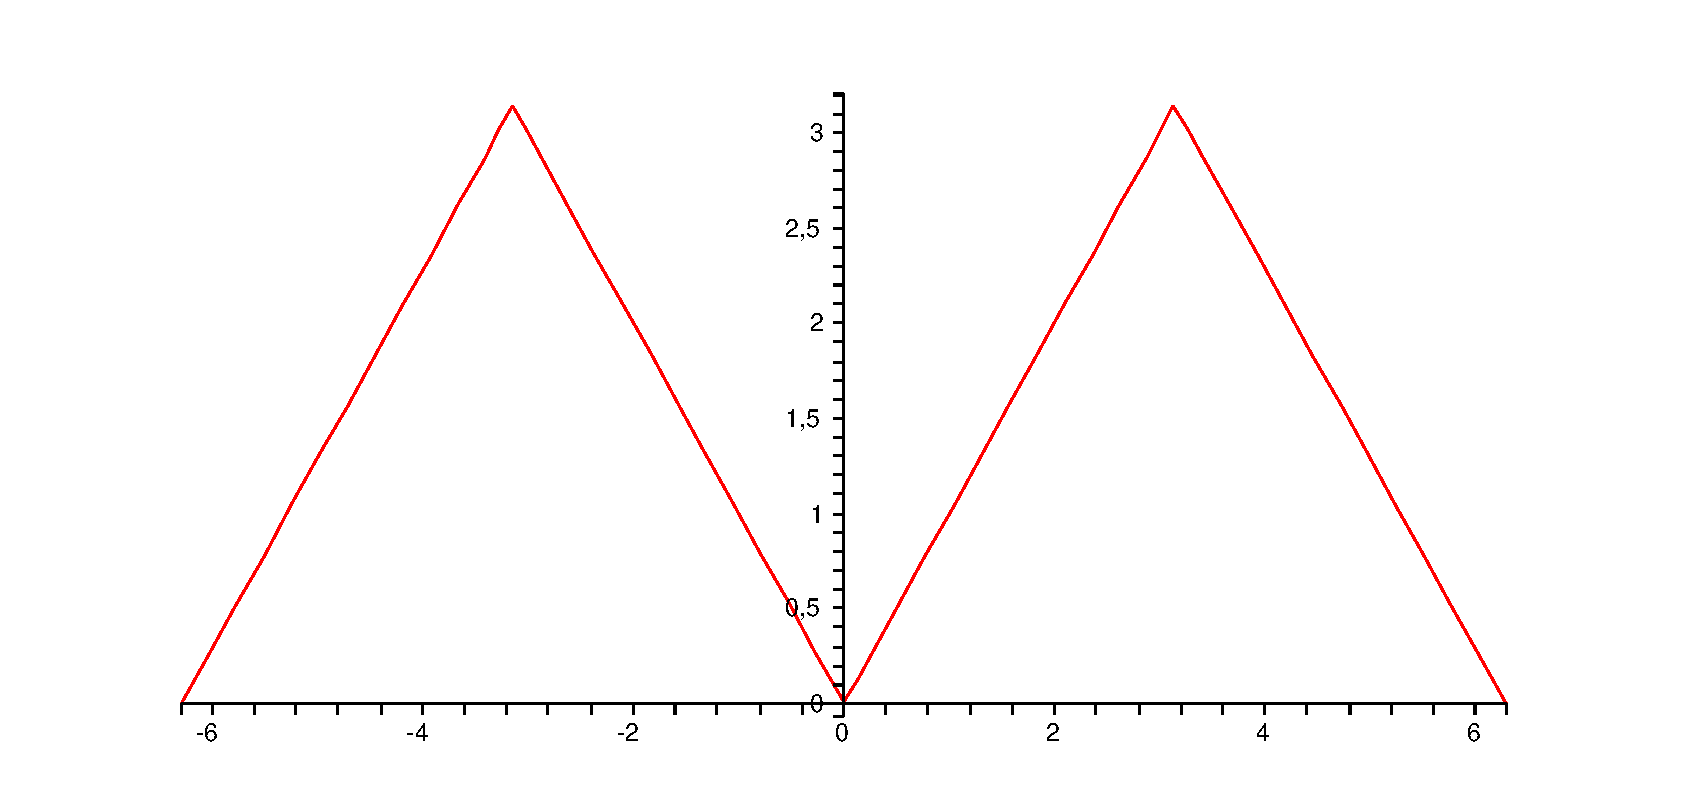
\epsfig{file=Figures/saegezahn.eps,scale=0.5}
   \caption{Die S�gezahn-Funktion.}
  \label{fig:saegezahn.eps}
\end{figure}
\begin{enumerate}
\item Die Koeffizienten $a_n$ ergeben sich als 
      \\[0.3cm]
      \hspace*{0.5cm}
      $\displaystyle
        a_n  =  \bruch{1}{\pi} \cdot\int_0^{2\cdot\pi} s(x) \cdot \cos(n\!\cdot\!x)\,dx 
             =  \bruch{2}{\pi} \cdot\int_{0}^{\pi} s(x) \cdot \cos(n\!\cdot\!x)\,dx
             =  \bruch{2}{\pi} \cdot\int_{0}^{\pi} x \cdot \cos(n\!\cdot\!x)\,dx, 
      $
      \\[0.3cm]
      denn die Funktion $x \mapsto s(x) \cdot \cos(n\!\cdot\!x)\,dx$ ist einerseits
      periodisch mit der Periode $2\cdot\pi$ und andererseits gerade.
      Im Falle $n=0$ haben wir 
      \\[0.1cm]
      \hspace*{1.3cm}
        $\displaystyle a_0 = \bruch{2}{\pi} \cdot\int_{0}^{\pi} x \cdot \cos(0\!\cdot\!x)\,dx =
          \bruch{2}{\pi} \cdot\int_{0}^{\pi} x \,dx = 
          \bruch{2}{\pi} \cdot \bruch{x^2}{2} \,\bigg|_0^\pi = \bruch{2}{\pi} \cdot \bruch{\pi^2}{2} =\pi$.
      \\[0.1cm]
      Andernfalls berechnen wir das Integral  mit Hilfe partieller Integration.  Wir setzen
      $v'(x) = \cos(n\!\cdot\!x)$ und $u(x) = x$.  Dann gilt
      $v(x) = \frac{1}{n}\cdot \sin(n\!\cdot\!x)$ und $u'(x) = 1$, also haben wir f�r 
      $n \geq 1$
      \\[0.3cm]
      \hspace*{1.3cm}
      $
      \begin{array}[t]{lcl}
         a_n &= &\displaystyle \bruch{2}{\pi} \cdot\left( x \cdot \bruch{1}{n}\sin(n\!\cdot\!x) \bigg|_0^{\pi} - 
               \bruch{1}{n}\cdot \int_0^{\pi} \sin(n\!\cdot\!x)\,dx\right) \\[0.5cm]
             &= &\displaystyle \bruch{2}{\pi} \cdot\left(0 - \bruch{1}{n^2} \cdot \cos(n\!\cdot\!x)\, \bigg|_0^\pi\right) \\[0.5cm]
             &= &\displaystyle \bruch{2}{\pi} \cdot\bruch{1}{n^2}\cdot \Bigl( (-1)^n - 1 \Bigr), 
      \end{array}
      $
      \\[0.3cm]
      denn $\cos(n\cdot \pi) = (-1)^n$. Damit haben wir insgesamt
      \\[0.3cm]
      \hspace*{1.3cm}
      $a_0 = \pi$, \quad $a_{2\cdot n+1} = \bruch{-4}{\pi\cdot n^2}$ \quad und \quad $a_{2\cdot(n+1)} = 0$ \quad f�r $n\in \mathbb{N}$.
\item Die Koeffizienten $b_n$ ergeben sich als
      \\[0.3cm]
      \hspace*{1.3cm}
      $b_n  = \displaystyle \bruch{1}{\pi} \cdot\int_0^{2\cdot\pi} s(x) \cdot \sin(n\!\cdot\!x)\,dx = 0$
      \\[0.3cm]
      denn die Funktion $s(x) \cdot \sin(n\!\cdot\!x)$ ist sowohl periodisch mit der Periode $2\cdot\pi$ als auch ungerade.
\end{enumerate}
Insgesamt haben wir jetzt die Formel 
\\[0.3cm]
\hspace*{1.3cm}
$\displaystyle s(x) = \bruch{\pi}{2} - \bruch{4}{\pi} \cdot\sum\limits_{k=0}^\infty \bruch{1}{(2\!\cdot\!k+1)^2} \cdot \cos\bigl((2\!\cdot\!k+1)\cdot x\bigr)$
\\[0.3cm]
gefunden.  Setzen wir hier f�r $x$ den Wert $\pi$ ein, so ergibt sich wegen $\cos\bigl((2\!\cdot\!k+1)\cdot \pi\bigr) = - 1$
\\[0.1cm]
\hspace*{1.3cm}
$
\begin{array}[t]{clcl}
                & \pi & = & \bruch{\pi}{2} - \bruch{4}{\pi} \cdot\sum\limits_{k=0}^\infty \bruch{1}{(2\!\cdot\!k+1)^2} \cdot \cos\bigl((2\!\cdot\!k+1)\cdot \pi\bigr) \\[0.5cm]
\Leftrightarrow & \bruch{\pi}{2} & = &  \bruch{4}{\pi} \cdot\sum\limits_{k=0}^\infty \bruch{1}{(2\!\cdot\!k+1)^2} \\[0.5cm]
\Leftrightarrow & \bruch{\pi^2}{8} & = & \displaystyle \sum\limits_{k=0}^\infty \bruch{1}{(2\!\cdot\!k+1)^2}.
\end{array}
$
\\[0.3cm]
Damit sind wir jetzt in der Lage, die Reihe 
\\[0.2cm]
\hspace*{1.3cm}
$\sigma := \sum\limits_{n=1}^\infty \bruch{1}{n^2}$
\\[0.2cm]
zu berechnen.  Zun�chst zerlegen wir die Reihe in einen Teil, der nur �ber die geraden Indices 
l�uft und einen Teil, der �ber die ungeraden Indices l�uft: 
\\[0.3cm]
\hspace*{1.3cm}
$
\begin{array}[t]{clcl}
                & \sigma & = & \displaystyle 
                  \sum\limits_{n=1}^\infty \bruch{1}{(2\!\cdot\!n)^2} \;+\; \sum\limits_{n=0}^\infty \bruch{1}{(2\!\cdot\!n+1)^2} \\[0.5cm]
\Leftrightarrow & \sigma & = & \displaystyle 
                  \bruch{1}{4}\cdot\sum\limits_{n=1}^\infty \bruch{1}{n^2} \;+\; \bruch{\pi^2}{8} \\[0.5cm]
\Leftrightarrow & \sigma & = & \displaystyle \bruch{1}{4} \cdot \sigma  \;+\; \bruch{\pi^2}{8} \\[0.3cm]
\Leftrightarrow & \bruch{3}{4}\cdot\sigma & = & \bruch{\pi^2}{8} \\[0.3cm]
\Leftrightarrow & \sigma & = & \bruch{\pi^2}{6} 
\end{array}
$
\\[0.3cm]
Damit haben wir also die Formel 
\\[0.3cm]
\hspace*{1.3cm} $\sum\limits_{n=1}^\infty \bruch{1}{n^2} = \bruch{\pi^2}{6}$
\\[0.3cm]
gezeigt.  Die Frage nach dem Wert dieser Reihe war 1644 als \emph{Basel'sches Problem} von
Pietro Mengoli gestellt worden. 
F�hrende Mathematiker des 17-ten Jahrhunderts hatten sich erfolglos mit dieser Frage
besch�ftigt.
Im Jahre 1735 gelang es Leonard Euler (1707 - 1783), dieses Problem zu l�sen.
\pagebreak

\exercise
Die Funktion $p$ sei auf dem Intervall $[-\pi,\pi]$ definiert durch
\\[0.1cm]
\hspace*{1.3cm}
$p(x) = x^2$.
\\[0.1cm]
Die Funktion werde so auf $\mathbb{R}$ fortgesetzt, dass die resultierende Funktion die Periode
$2\!\cdot\!\pi$ hat.  
\begin{enumerate}
\item Berechnen Sie die Fourier-Reihe von $p$.
\item Berechnen Sie mit Hilfe der Fourier-Reihe von $p$ einen Wert f�r die Reihe
      \\[0.3cm]
      \hspace*{1.3cm}
      $\displaystyle \sum\limits_{n=1}^\infty \bruch{1}{n^2}$. 
\end{enumerate}



%%% Local Variables: 
%%% mode: latex
%%% TeX-master: "analysis"
%%% End: 

\chapter{Rundungsfehler}
Die meisten komplexen Probleme lassen sich nur mit numerischen Verfahren l�sen.  Wir haben
bereits verschiedene numerische Verfahren kennengelernt, beispielsweise Verfahren zur
Berechnung von Nullstellen sowie Verfahren zur numerischen Integration.  Allen diesen
Verfahren ist gemeinsam, dass zwei verschiedene Arten von Fehlern auftreten:
\begin{enumerate}
\item Ein \emph{Approximations-Fehler} tritt auf, wenn wir einen Wert $\lambda$ berechnen
      wollen, zu dessen Berechnung wir nur eine N�herungsformel existiert.  Oft ist der
      Approximations-Fehler ein \emph{Abbruch-Fehler}, der seine
      Ursache darin hat, dass wir nur endlich viele Glieder einer unendlichen Reihe
      berechnen k�nnen.  Wollen wir beispielsweise die Euler'sche Zahl $e$ nach der Formel
      \\[0.2cm]
      \hspace*{1.3cm}
      $e = \sum\limits_{k=0}^\infty \bruch{1}{k!}$
      \\[0.2cm]
      berechnen, so k�nnen wir auf dem Rechner diese Summe nicht gegen unendlich laufen
      lassen, sondern m�ssen die Summe nach endlich vielen Gliedern abbrechen, wir berechnen
      also als Approximation f�r $e$ eine Reihe der Form
      \\[0.2cm]
      \hspace*{1.3cm}
      $e_n := \sum\limits_{k=0}^n \bruch{1}{k!}$ 
      \\[0.2cm]
      und m�ssen dann $n$ so gro� w�hlen, dass der Abbruch-Fehler
      \\[0.2cm]
      \hspace*{1.3cm}
      $e - e_n = \sum\limits_{k=n+1}^\infty \bruch{1}{k!}$ 
      \\[0.2cm]
      unterhalb einer vorgegeben Schranke bleibt.
\item Zus�tzlich zum Approximations-Fehler gibt es noch die Rundungsfehler, die im Laufe der Rechnung 
      entstehen.  Diese Rundungsfehler haben Ihre Ursache darin, dass Flie�komma-Zahlen auf dem Rechner 
      mit einer vorgegebenen Genauigkeit dargestellt werden.  Rechnen wir in der Sprache \textsl{Java}
      mit einer Flie�komma-Zahl vom Typ \texttt{float}, so stehen zur Darstellung der Stellen hinter dem
      Komma lediglich 23 Bits zur Verf�gung.  Werden nun zwei solche Zahlen multipliziert, so k�nnten
      bis zu 47 Bits notwendig sein, um alle Stellen hinter dem Komma korrekt wiedergeben zu k�nnen.
      Da aber zum Abspeichern des Ergebnisses lediglich 23 Bits zur Verf�gung stehen, um die Ziffern 
      hinter dem Komma abzuspeichern, bleibt nichts anderes �brig, als das Ergebnis auf 23 Bits zu
      runden.  Der dadurch entstehende Fehler wird als Rundungsfehler bezeichnet.
\end{enumerate}
Die Auswirkungen von Rundungsfehlern werden oft untersch�tzt.  Unter
\\[0.2cm]
\hspace*{1.3cm}
\texttt{http://www.devtopics.com/20-famous-software-disasters-part-2/}
\\[0.2cm]
findet sich eine Liste der 20 spektakul�rsten Software-Fehler, die Katastrophen ausgel�st haben.
In mehreren F�llen waren Rundungsfehler ein Teil des Problems.  Um einen ersten Eindruck von der Wirkung
von Rundungsfehlern zu bekommen, betrachten wir das in Abbildung \ref{fig:harmonic.stlx} gezeigte
Programm zur Berechnung der Reihe
\\[0.2cm]
\hspace*{1.3cm}
$\sum\limits_{n=1}^\infty \bruch{1}{n}$.

\begin{figure}[!ht]
\centering
\begin{Verbatim}[ frame         = lines, 
                  framesep      = 0.3cm, 
                  firstnumber   = 1,
                  labelposition = bottomline,
                  numbers       = left,
                  numbersep     = -0.2cm,
                  xleftmargin   = 0.8cm,
                  xrightmargin  = 0.8cm,
                ]
    harmonic := procedure() {
        oldSum := 0.0;
        sum := 1.0;
        n := 1;
        while (oldSum < sum) {
            oldSum := sum;
            n += 1;
            sum += 1/n;
        }
        print("sum = $sum$, n = $n$");
    };    
    harmonic();
\end{Verbatim}
\vspace*{-0.3cm}
\caption{Berechnung von $\sum\limits_{n=1}^\infty \bruch{1}{n}$.}
\label{fig:harmonic.stlx}
\end{figure}

Sie erwarten jetzt vielleicht, dass diese Programm nie terminiert, aber wenn wir dieses Programm
in einer Datei mit dem Namen ``\texttt{harmonic.stlx}'' speichern und es dann mit dem Befehl
\\[0.2cm]
\hspace*{1.3cm}
\texttt{setlX --real32 harmonic.stlx}
\\[0.2cm]
starten, dann erhalten wir nach wenigen Sekunden die Meldung:
\\[0.2cm]
\hspace*{1.3cm}
\texttt{sum = 13.05426, n = 200001}.
\\[0.2cm]
Da wir fr�her bewiesen haben, dass die Partialsummen $\sum\limits_{k=1}^n \bruch{1}{k}$ f�r wachsende Werte
von $n$ beliebig gro� werden, fragen wir uns, was bei der Rechnung schief gelaufen ist.
Die Antwort ist, dass f�r $n= 200001$ der Wert $\frac{1}{n}$ so klein ist, dass die Summe
\\[0.2cm]
\hspace*{1.3cm}
$13.05426 + \frac{1}{n}$
\\[0.2cm]
so nahe bei $13.05426$ liegt, dass sie auf den Wert $13.05426$ abgerundet wird.  Um diesen Effekt n�her
zu beschreiben, definiert man f�r einen vorgegebenen Rechner die sogenannte
\emph{Maschinen-Konstante} \textsl{eps} als die kleinste positive Zahl, die, wenn sie auf diesem Rechner zu
$1$ addiert wird, eine Ergebnis gr��er als 1 ergibt.  Die formale Definition lautet
\\[0.2cm]
\hspace*{1.3cm}
$\textsl{eps} := \min\bigl( \{ x \in \mathbb{R} \mid x > 0 \wedge 1 \oplus x > 1 \} \bigr)$.
\\[0.2cm]
Hier bezeichnet $\oplus$ die auf dem Rechner implementierte Addition.
Abbildung \ref{fig:maschinen-konstante.stlx} zeigt ein einfaches Programm zur Berechnung der
Maschinen-Konstante.  Bei der im \textsc{Ieee}-Standard 754 definierten 32-Bit-Architektur erhalten wir
f�r $\textsl{eps}$ den Wert
\\[0.2cm]
\hspace*{1.3cm}
$\textsl{eps}_{32} = 9.536745 \cdot 10^{-7}$,
\\[0.2cm]
bei einer 64-Bit-Architektur lautet das Ergebnis
\\[0.2cm]
\hspace*{1.3cm}
$\textsl{eps}_{64} = 8.88178419700125 \cdot 10^{-16}$,
\\[0.2cm]
und wenn wir mit 128-Bit rechnen, haben wir
\\[0.2cm]
\hspace*{1.3cm}
$\textsl{eps}_{128} = 7.703719777548943412223911770339695 \cdot 10^{-34}$.
\vspace*{0.3cm}

\begin{figure}[!ht]
\centering
\begin{Verbatim}[ frame         = lines, 
                  framesep      = 0.3cm, 
                  firstnumber   = 1,
                  labelposition = bottomline,
                  numbers       = left,
                  numbersep     = -0.2cm,
                  xleftmargin   = 0.8cm,
                  xrightmargin  = 0.8cm,
                ]
    maschinenKonstante := procedure() {
        eps := 1.0;
        old := eps;
        while (1.0 + eps > 1.0) {
            old := eps;
            eps /= 2;
        }
        return old;
    };
\end{Verbatim}
\vspace*{-0.3cm}
\caption{Berechnung der Maschinen-Konstante \textsl{eps}.}
\label{fig:maschinen-konstante.stlx}
\end{figure}

\noindent
Bei modernen Rechnern, die den \textsc{Ieee}-Standard 754 implementieren, k�nnen wir davon ausgehen, dass
der relative Rundungsfehler bei der Ausf�hrung 
einer  Grundrechenoperation durch die Maschinen-Konstante \textsl{eps} beschr�nkt ist.

Leider muss die Vorlesung aus Zeitgr�nden an dieser Stelle enden.  Der interessierten Leser sei daher
auf die Literatur, insbesondere den Artikel von Goldberg \cite{goldberg:91} verwiesen. 

%%% Local Variables: 
%%% mode: latex
%%% TeX-master: "analysis"
%%% End: 


%\bibliographystyle{alpha}
\bibliography{cs}
%\bibliography{/Users/stroetma/Dropbox/Kurse/cs}

\end{document}



